 \documentclass[sigplan,review,anonymous]{acmart}
 \acmSubmissionID{370} %TODO: Update this after submitting the abstract.
 \renewcommand\footnotetextcopyrightpermission[1]{}
 % Optional: Remove the ACM reference between the abstract and the main text.
 \settopmatter{printfolios=true,printacmref=false}
 % Optional: Comment out the CCS concepts and keywords.

%\documentclass[sigconf, nonacm]{acmart}
%
%%% The following content must be adapted for the final version
%% paper-specific
%\newcommand\vldbdoi{XX.XX/XXX.XX}
%\newcommand\vldbpages{XXX-XXX}
%% issue-specific
%\newcommand\vldbvolume{17}
%\newcommand\vldbissue{1}
%\newcommand\vldbyear{2023}
%% should be fine as it is
%\newcommand\vldbauthors{\authors}
%\newcommand\vldbtitle{\shorttitle} 
%% leave empty if no availability url should be set
%\newcommand\vldbavailabilityurl{}
%%\newcommand\vldbavailabilityurl{URL_TO_YOUR_ARTIFACTS}
%% whether page numbers should be shown or not, use 'plain' for review versions, 'empty' for camera ready
%\newcommand\vldbpagestyle{plain}

\usepackage[utf8]{inputenc}
\usepackage{times}
\usepackage{graphicx}
\usepackage{xcolor}
\usepackage{hyperref}
\usepackage{paralist}
\usepackage{listings}
\usepackage[inline]{enumitem}

\usepackage{microtype} % character spacing

\usepackage{booktabs} %added for tables (Andre)
\usepackage{algorithm}
\usepackage[noend]{algpseudocode}
\usepackage{svg}

\usepackage{xparse}
\makeatletter
\NewDocumentCommand{\LeftComment}{s m}{%
	\Statex \IfBooleanF{#1}{\hspace*{\ALG@thistlm}}\(\triangleright\) #2}
\makeatother

\definecolor{dkgreen}{rgb}{0,0.6,0}
\definecolor{gray}{rgb}{0.5,0.5,0.5}
\definecolor{mauve}{rgb}{0.58,0,0.82}
\lstset{language=SQL,
  basicstyle={\scriptsize\ttfamily},
  deletekeywords={key}, %not working
  belowskip=0mm,
  breakatwhitespace=true,
  breaklines=true,
  classoffset=0,
  columns=flexible,
  commentstyle=\color{dkgreen},
  framexleftmargin=0.25em,
  frameshape={}{}{}{},
  %frameshape={}{yy}{}{}, %To remove to vertical lines on left, set `frameshape={}{}{}{}`
  keywordstyle=\color{blue},
  numbers=none, %If you want line numbers, set `numbers=left`
  numberstyle=\tiny\color{gray},
  showstringspaces=false,
  stringstyle=\color{mauve},
  tabsize=3,
  xleftmargin =0em
}

\newcommand{\qcr}[1]{{\fontfamily{qcr}\selectfont #1}}
\newcommand{\code}[1]{\textsf{\small{#1}}}


\usepackage{balance}  % for  \balance command ON LAST PAGE  (only there!)

\usepackage{subcaption}
\graphicspath{{./images/}}

%Makes compact lists a little bit less compact
\setlength{\pltopsep}{0.3em}
\setlength{\plitemsep}{0.1em}

%\newcommand{\grumbler}[2]{{\color{red}{\bf #1:} #2}}
%\renewcommand{\grumbler}[2]{}
%\newcommand{\andre}[1]{\grumbler{andre}{#1}}
%\newcommand{\nuno}[1]{\grumbler{nuno}{#1}}
%\newcommand{\carla}[1]{\grumbler{carla}{#1}}

\newcommand{\outline}[1]{}
%\newcommand{\outline}[1]{\grumbler{outline}{#1}}

\newcommand{\emphvspace}{0.5\baselineskip}
%Single line
\newcommand{\lineemph}[1]{\vspace{\emphvspace}\hspace{2em}\emph{#1}\vspace{\emphvspace}}
%Multi line
\newcommand{\firstblockemph}[1]{\vspace{\emphvspace}\hspace{2em}\emph{#1}}
\newcommand{\middleblockemph}[1]{\hspace{2em}\emph{#1}}
\newcommand{\lastblockemph}[1]{\hspace{2em}\emph{#1}\vspace{\emphvspace}}
\newcommand{\emphfunction}[2]{\emph{#1}($#2$)}

\newtheorem{theorem}{Theorem}

\lstset{columns=fullflexible,
        mathescape=true,
        literate=
               {=}{$\leftarrow{}$}{1}
               {==}{$={}$}{1},
        morekeywords={fun}
        }

\definecolor{red}{RGB}{200,0,0}
\definecolor{green}{RGB}{0,200,0}
\definecolor{blue}{RGB}{0,0,200}
\usepackage{ifthen}
\newboolean{showcomments}
\setboolean{showcomments}{false} %
\ifthenelse{\boolean{showcomments}}
{\newcommand{\nbnote}[3]{
  %
  \fcolorbox{gray}{yellow}{\bfseries\sffamily\scriptsize#1}
  {\color{#2} \sffamily\small$\blacktriangleright$\textit{#3}$\blacktriangleleft$}
%
  %
  }
}
{\newcommand{\nbnote}[3]{}
 \newcommand{\version}{}
}
\newcommand{\andre}[1]{\nbnote{Andre}{blue}{#1}}
\newcommand{\carla}[1]{\nbnote{Carla}{green}{#1}}
\newcommand{\nuno}[1]{\nbnote{Nuno}{red}{#1}}

\begin{document}

%\showthe\columnwidth
%\showthe\textwidth
%\showthe\linewidth

\title{Global Views on Partially Geo-Replicated Data}

%%
%% The "author" command and its associated commands are used to define the authors and their affiliations.
%
%\author{André Rijo, Carla Ferreira, Nuno Preguiça}
%\affiliation{
%\institution{NOVA LINCS, FCT, Universidade NOVA de Lisboa}
%\country{Portugal}
%}

%I used this example provided by VLDB:
%\author{Wang Xiu Ying}
%\author{Zhe Zuo}
%\affiliation{%
%	\institution{East China Normal University}
%	\city{Shanghai}
%	\country{China}
%}
%\email{firstname.lastname@ecnu.edu.cn}

%Maybe the mails should be used separately too as in their example?
%\author{J\"org von \"Arbach}
%\affiliation{%
%	\institution{University of T\"ubingen}
%	\city{T\"ubingen}
%	\country{Germany}
%}
%\email{jaerbach@uni-tuebingen.edu}
%\email{myprivate@email.com}
%\email{second@affiliation.mail}

%Note: from VLDB's guidelines: "list every author in its own author tag. The authors can, as shown in the template sample, share the same affiliations, but every author deserves his/her own author tag! There may not be any Additional Authors section."
\author{André Rijo}
\author{Nuno Preguiça}
\author{Carla Ferreira}
\affiliation{%
	\institution{NOVA LINCS, NOVA School of Science and Technology, FCT NOVA}
	\city{Almada}
	\country{Portugal}
}
%\email{a.rijo@campus.fct.unl.pt}
%\email{{nuno.preguica,carla.ferreira}@fct.unl.pt}
%\email{a.rijo@campus.fct.unl.pt, \{nuno.preguica,carla.ferreira\}@fct.unl.pt}

\begin{abstract}


Geo-replication is a key technique for providing low latency and high
availability in global services. As the number of data centers increases, so does the replication cost of full replication, which 
makes partial replication an attractive approach.

This paper presents PotionDB, a novel geo-distributed, partially replicated key-value store.  
PotionDB transaction management and replication algorithms provide transactional causal consistency 
for transactions that access local and remote objects. 
To enable the support of recurrent queries over geo-partitioned data, PotionDB provides
efficient materialized views, that allow these queries to be replied locally at all replicas.
Our evaluation shows that queries concerning global data can be completed in less than one millisecond 
while maintaining high throughput, despite the extra operations required to keep views up-to-date. 


%Many existing web services at a global scale have strict latency, availability, and fault tolerance requirements.
%To address these requirements,  services are often deployed in data centers distributed 
%across the globe, with users accessing the closest data center.
%As the number of servers increases, so does the replication cost, which makes partial replication an attractive approach.
%However, some queries may require data not replicated in every server (e.g. in an e-commerce system, the best-selling products across the globe).
%
%In this paper, we present PotionDB, a novel geo-distributed key-value store that provides partial replication.
%We present a replication scheme that allows data to be partially replicated, yet still, answer queries relative to global data efficiently.
%We leverage existing partial and non-uniform replication algorithms to provide materialized views of data that may be split across multiple servers.
%With these views, a client can obtain global information by querying a single server.
%Our evaluation shows that queries concerning global data can be completed in less than one millisecond while maintaining high throughput, despite the extra operations required to keep views up-to-date. 


\end{abstract}

\maketitle

%%% do not modify the following VLDB block %%
%%% VLDB block start %%%
%\pagestyle{\vldbpagestyle}
%\begingroup\small\noindent\raggedright\textbf{PVLDB Reference Format:}\\
%\vldbauthors. \vldbtitle. PVLDB, \vldbvolume(\vldbissue): \vldbpages, \vldbyear.\\
%\href{https://doi.org/\vldbdoi}{doi:\vldbdoi}
%\endgroup
%\begingroup
%\renewcommand\thefootnote{}\footnote{\noindent
%	This work is licensed under the Creative Commons BY-NC-ND 4.0 International License. Visit \url{https://creativecommons.org/licenses/by-nc-nd/4.0/} to view a copy of this license. For any use beyond those covered by this license, obtain permission by emailing \href{mailto:info@vldb.org}{info@vldb.org}. Copyright is held by the owner/author(s). Publication rights licensed to the VLDB Endowment. \\
%	\raggedright Proceedings of the VLDB Endowment, Vol. \vldbvolume, No. \vldbissue\ %
%	ISSN 2150-8097. \\
%	\href{https://doi.org/\vldbdoi}{doi:\vldbdoi} \\
%}\addtocounter{footnote}{-1}\endgroup
%%%% VLDB block end %%%
%
%%%% do not modify the following VLDB block %%
%%%% VLDB block start %%%
%\ifdefempty{\vldbavailabilityurl}{}{
%	\vspace{.3cm}
%	\begingroup\small\noindent\raggedright\textbf{PVLDB Artifact Availability:}\\
%	The source code, data, and/or other artifacts have been made available at \url{\vldbavailabilityurl}.
%	\endgroup
%}
%%%% VLDB block end %%%

\section{Introduction}
\label{sec:introduction}

%	\item Num. DC a aumentar

The increasing reliance on web services in many domains of activity leads to stringent requirements regarding latency, availability,
and fault tolerance~\cite{Schurman2009latency,gomez}.
To address these requirements, cloud platforms have been adding new data centers at different geographic 
locations. By allowing users to contact the closest data center, a global service can
provide low latency to users spread across the globe. 
The increasing number of data centers also contributes
for providing high availability,  as an user can access any
available data center.

% serviços necessitam de data
% Replicar totalmente tem problemas

Global services running at multiple geographic locations need 
to rely on a geo-replicated database~\cite{dynamo}.
%A number of geo-replicated databases have been proposed, providing different consistency semantics.
Databases~\cite{spanner,cockroachdb,mdcc} that provide strong consistency give the illusion that 
a single replica exists, requiring coordination among
replicas for executing (update) operations. This leads to high latency and may compromise 
availability in the presence of network partitions.
Databases that provide weak consistency~\cite{eventual,dynamo,cops} allow any replica to process a
client request, leading to lower latency and high availability. As a consequence, these databases expose
temporary state divergence to clients, making it more difficult to program a system. 

In either case, geo-replicated databases usually adopt a full replication model, where each data 
center replicates the full database. 
As both the data managed by these systems and the number of data centers increases,
this approach leads several problems.
First, storing all data in all data centers imposes a large overhead in terms of storage. 
Furthermore, storing all data in all data centers may be unnecessary, as some data is only needed at some
geographic locations.
Second, increasing the number of replicas makes replication 
%process 
more complex and costly, 
as each update needs to be propagated to all replicas.

For addressing these problems, partial replication is an attractive approach, with each data center
replicating only a subset of the data.
A number of works have been addressing the challenges of 
partial replication, for example by proposing algorithms to manage partially 
replicated data~\cite{spanner,saturn,sipre, practi} and to decide which data is replicated in each replica~\cite{slog, sipre}.

This paper addresses the problem of querying data in a weakly consistent partially geo-replicated database, 
focusing on recurrent queries. % for which the application could use a (materialized) view.
For example, consider an e-commerce system with users from multiple geographic locations.
In this case, the data pertaining users of a given location does not need to be replicated in all data centers
(but only in a few for fault tolerance). The same applies to other information, such as data on orders and 
warehouses.
Other data, such as information on products would be replicated in the regions where the product
is available for sale.  
Under this data placement, computing the list of best seller products is challenging, as it requires
accessing data located at multiple data centers.

This problem can be addressed using different approaches. 
First, it is possible to have a \emph{main} data center that replicates all data, and forward queries to such data center.
This makes the \emph{main} data center a central point of failure and a performance bottleneck, as it needs to execute all these queries.
Second, it is possible to execute the query by accessing multiple locations,  using, for example, 
a distributed processing system for geo-partitioned data~\cite{kloudas2015pixida,jetstream}.
This requires running an additional external service, posing challenges for the consistency of the results returned and the data returned
in other queries.
%, mostly when adopting weak consistency models (a local update that should
%be reflected in the result of the query may not be returned, as the update might have not been read by the 
%external service that accessed a different replica).

We propose a different approach: to maintain materialized views, as commonly available in centralized 
relational databases.
Implementing such feature efficiently in a partially geo-replicated database requires 
addressing two main challenges. 
First, it is necessary to maintain the materialized views consistent with the remaining data
accessed by the application. 
To achieve this, we designed mechanisms for transaction execution and replication where updates 
to the base data and views are made visible atomically in each replica.

Second, it is necessary to efficiently support materialized views. 
As many recurrent queries include aggregations or limits (e.g. TPC-H~\cite{tpch} queries)
%all defined queries use aggregations or limits
it is particularly important to support
this type of views. We have designed an incremental view maintenance 
mechanism that builds and extends 
Non-uniform Conflict-free Replicated Data Types (NuCRDTs)~\cite{Cabrita17Nonuniform}, 
a CRDT~\cite{crdt} model where each replica can maintain a different state as long as the 
the results of reads is the same in all replicas. 

%crdt} and non-uniform replication~\cite{Cabrita17Nonuniform}.
%While CRDTs allow updates to views to be performed in any replica, the latter minimizes
%the updates propagated to other replicas to only those that might influence the final result.


%limits, used for example to support \emph{topK} 
%queries.
%To achieve this, we build on the concept of non-uniform replication \cite{Cabrita17Nonuniform}, in which the state
%of different replicas may be different, given that the observable state is (eventually) the same.
%This allows each replica to propagate only the updates that might be relevant to the observable 
%state. Providing support for views required us to extend non-uniform replication from simple data 
%types to more complex structures that could support a view with multiple columns.

We present the design and implementation of PotionDB, a geo-replicated memory key-value store with support  
for partial replication and materialized views. 
PotionDB provides weak consistency, for improved latency and availability,  with transactional 
causal consistency~\cite{cure}, for improved consistency.
Views are kept up-to-date with the base data. 
% without requiring any extra coding or update logic from 
%the application programmer.
%Maybe mention about how the view is kept up-to-date even without any of the base data present in the replica?  
To our knowledge, our work is the first to address the problem of maintaining materialized views in such setting.  

\andre{We'll need to review the paragraph below after the evaluation section is ``finished for good''}

PotionDB was evaluated with \mbox{TPC-H} queries~\cite{tpch} and micro-benchmarks.
The results show that PotionDB provides much better performance to answer recurrent queries
than alternatives.
% approaches.  
Performance scales almost linearly with the number of replicas. % in the system.
Further, the overhead of maintaining materialized views is low, increasing slightly with
\mbox{the ratio of updates.}

% for maintaining materialized views impose 
%low overhead when executing asynchronously replicating transactions, particularly
%for views with limits. 
%\nuno{deviamos ter uns micro-benchmarks que comparassem o overhead com limites e sem limites}
%%Additionally, the results show that executing queries by relying on the materialized views is much more 
%%efficient than using alternative mechanisms.  
%Moreover, our algorithms for maintaining materialized views in a decentralized way perform better 
%than alternative approaches where the view is computed in a single data center, 
%while also keeping consistency between the base and view data in every replica.



In this paper we make the following contributions:
%\begin{enumerate*}[(label=\roman*)]
\begin{itemize}[noitemsep,topsep=0pt,parsep=0pt,partopsep=0pt,leftmargin=*]
	\item 
	%design of a 
	the design of a partially geo-replicated key-value store with 
	views over geo-partitioned data (Section~\ref{sec:transactions}); 
	\item replication algorithms that efficiently maintain consistent materialized views over 
	partially replicated data (Section~\ref{sec:views_for_apps});
%	\item a language inspired in SQL for view specification in key-value stores, with view maintenance code automatically inferred from the specification;
	 \item implementation and evaluation of the proposed approach with TPC-H and micro-benchmarks
	 (Section~\ref{sec:evaluation}).
\end{itemize}

%The remainder of the paper is organized as follows.
%Section~\ref{sec:overview} presents the system model, as well as PotionDB's architecture, consistency guarantees and API. %System model? Or Data Model?
%Section~\ref{sec:transactions} describes PotionDB's transactional and replication protocols.
%Section~\ref{sec:views_for_apps} discusses details on how PotionDB generates views and their automatic updating, as well as how we adapted TPC-H to PotionDB.
%%Section~\ref{sec:views_for_apps} discusses how we adapted TPC-H to PotionDB, exemplifies how views can be specified given a query and discusses some details on how PotionDB generates views and their automatic updating.
%In Section~\ref{sec:evaluation} we experimentally evaluate PotionDB using TPC-H and micro-benchmarks, while Section~\ref{sec:related_work} presents related work and Section~\ref{sec:conclusion} concludes.
%\andre{On the description of Section \ref{sec:views_for_apps}, maybe change "their automatic updating" to "keeps them automatically up-to-date"?}


%\outline{topicos
%
%\begin{itemize}
%	\item Num. DC a aumentar
%	\item Replicar totalmente tem problemas
%	\item Replicação parcial
%	\item Queries sobre dados replicados parcialmente
%	\begin{itemize}
%		\item Standard solution?
%	\end{itemize}
%	\item Views materializadas replicadas totalmente
%	\item Contribuições
%\end{itemize}
%}

\section{System Overview}
\label{sec:overview}

This section overviews PotionDB, focusing on support for 
recurrent queries.

PotionDB is a distributed database designed for supporting global services deployed at multiple data centers. 
In these settings, (some) data items are only needed at some geographic locations. 
As a running example, we consider a large e-commerce site with online stores for different countries 
and clients spread across the world. 
The service includes data for products, with some products available 
only at some locations. The service maintains information about customers and their purchases, 
with clients being associated with one online store.

In this context, fully replicating the whole dataset might become too expensive.
Additionally, as most data is tied to some geographic location, one can expect that the majority of accesses
occurs on that location. 
PotionDB adopts partial geo-replication, with data items being replicated only at some locations.
This allows PotionDB to reduce replication cost when
compared to solutions featuring full replication, saving on both storage, processing, and networking costs.

While some application operations access data objects directly (e.g. user, product, or purchase objects),
other operations require data that results from an aggregation (e.g.  top
selling products worldwide)
%and users that bought some product).  
For supporting the latter, %operations,
PotionDB provides materialized views that are the result of an aggregation 
over geo-partitioned data and provides algorithms to efficiently maintain these views consistent.

The key features of this example - global service with a large database with
data that is mostly accessed in a single (or few) location,  and some operations accessing the result
of a global aggregation - are common to other global services, such as multi-user online games, and
social news aggregation.


%What do I want to define?
%Define formally objects and views.
%Define how objects are identified (key, bucket, type) and the idea of "objectID" (the triple). On the type, can define it generically (set, map, etc. Later can say those map to CRDT types)
%Define the API to process objects. Be short on the common parts of the API. Mention partial reads but in a generic form (give the example of set). Do not mention details on their workings - this will be somewhere else.
%Define the API to define views. I will need to think of this carefully, as we do not really have an API for this.
%Maybe can be something like saying views are just like normal objects... the detail is on how to keep them updated, and leave that for another section.

\subsection{Data model}
\label{subsec:datamodel}

PotionDB is a distributed key-value database.
We identify two types of values: base objects, $\mathit{Objs}$, and derived objects, $\mathit{Views}$.
The set of objects of a database is defined as $\mathit{DB} = \mathit{Objs} \cup \mathit{Views}$.
Informally, an object, $o$, is any value that is either a base object, $b$, or view, $v$.
We distinguish between base objects and views whenever necessary for clarity.

The value of a view is defined as a function over the values of other object(s), i.e., 
$\forall\, v \in \mathit{Views} : v = \mathit{fun}_v(D_v)$, 
where $D_v$ is the set of objects (potentially both base objects and other views) used to compute $v$.
We assume the computation is non-recursive, i.e., the value of a view is never based on its own value or, formally, 
$\forall\, v \in \mathit{Views} : v \notin D_v$.

Objects are uniquely identified by a tuple $\mathit{id} = \mathit{(key, bucket}$, $\mathit{type)}$.
%For presentation purposes, we assume this tuple is a property of the object and we define $\mathit{id} = \mathit{(key, bucket, type)}$.
%When needed, we represent these properties for an object $o$ as
%$o^{\mathit{id}}$, $o^{\mathit{key}}$, $o^{\mathit{bucket}}$, $o^{\mathit{type}}$.
Objects are stored in $\mathit{buckets}$, which are the unit of replication in PotionDB. 
Buckets are further logically grouped in containers. %, as further detailed in Section \ref{subsec:buckets}. 
An object has a $\mathit{key}$ inside the bucket.

PotionDB supports objects of different data types, including registers, counters, averages, sets, maps
and top-K objects~\cite{Cabrita17Nonuniform}.
Both base object and views are implemented as CRDTs~\cite{crdt}, guaranteeing that object replicas converge to a single state
in the presence of concurrent updates.

\subsection{Interface}
\label{subsec:interface}

%<<<<<<< HEAD
%\begin{table}[]
%	\setlength\tabcolsep{4pt}
%	\begin{tabular}{ll} 
%		\toprule
%		\hspace*{-0.35em}get(txId, id) $\rightarrow$ value                  & begin(clk) $\rightarrow$ txId            \\
%		\hspace*{-0.35em}read(txId, id, op) $\rightarrow$ value             & commit(txId) $\rightarrow$ clk           \\
%		\hspace*{-0.35em}update(txId, id, op) $\rightarrow$ ok           & rollback(txId) $\rightarrow$ ok                           \\
%		& \\
%		\hspace*{-0.35em}readTx(clk, read(s)) $\rightarrow$ clk, value(s) & updateTx(clk, update(s)) $\rightarrow$ clk \\
%=======
\begin{smaller}
\begin{table}[t]
\center
	\begin{tabular}{ll} 
		\toprule
		 \code{begin(clk) $\rightarrow$ txId}                    & \code{get(txId, id) $\rightarrow$ value}            \\
		 \code{commit(txId) $\rightarrow$ clk}            & \code{read(txId, id, op) $\rightarrow$ value}          \\
		  \code{rollback(txId) $\rightarrow$ ok}        & \code{upsert(txId, id, op) $\rightarrow$ ok}                        \\[4pt]
		\multicolumn{2}{l}{\code{oneShotTx(clk, (id, op)$^+$) $\rightarrow$ clk, value$^+$}} \\
	%	\multicolumn{2}{l}{\code{updateTx(clk, (id, op)$^+$) $\rightarrow$ clk}} \\
		%\multicolumn{2}{l}{\code{readTx(clk, read$^+$) $\rightarrow$ clk, value$^+$}} \\
		%\multicolumn{2}{l}{\code{updateTx(clk, update$^+$) $\rightarrow$ clk}} \\
		\bottomrule
	\end{tabular}
	%\vspace{0.8em}
	\caption{PotionDB's data manipulation API.}
	\label{table:PotionDB_API}
	\vspace{-20pt}
\end{table}
\end{smaller}

PotionDB offers a key-value  transactional interface, as summarized in Table \ref{table:PotionDB_API}.
An application issues interactive transactions, by executing \code{begin(clk)},
where \code{clk} is used to enforce causality between consecutive transactions.
A transaction proceeds with a sequence of operations: 
\begin{inparaenum}[(i)] 
\item \code{get(txId, id)}, which returns the full state of the object;
\item \code{read(txId, id,op)}, which returns the result of read-only operation \code{op} executed in the object; and
\item \code{upsert(txId, id,op)}, which updates object \code{id} by executing operation \code{op}, or creates the object if it does not exist.
%; 
%\item an object is deleted by issuing the \code{delete}  operation.
\end{inparaenum}
Operations defined in each object are type-specific - e.g. a set has a \code{contains(e)} operation to check
if value \code{e} belongs to the set, and an \code{add(e)} and \code{remove(e)} to add or remove \code{e} from the set.
A transaction ends with a \code{commit(txId)} for committing the transaction%, making updates durable,  
or \code{rollback(txId)} to abort the transaction.

%PotionDB also allows an application to issue an one-shot~\cite{eiger} read-only or write-only transaction,
PotionDB also supports one-shot transactions, \code{oneShotTx(clk, (id, op)$^+$)}, that include a sequence of read or
write operations.
%~\cite{??????} 
%read-only or write-only transaction,
%by executing, respectively, \code{readTx(clk, (id, op)$^+$)} or \code{updateTx(clk, (id, op)$^+$)}.
%for aborting 

PotionDB's data definition API includes operations to create and delete buckets, and 
to create views. Even if buckets have no associated
data type, i.e., any object type can be stored in any bucket, we expect that applications 
store objects of the same type in each bucket.  A document or a table row can be stored in 
PotionDB as a map CRDT, with each element of the map having its own type. 


\begin{figure}[t]
\small{
\begin{lstlisting}[language=SQL]
CREATE VIEW (MonthlyTopSales, views) WITH 
YEAR == ANY (SELECT DISTINCT SaleDate.Year FROM sales), 
MONTH ==  ANY (SELECT DISTINCT SaleDate.Month FROM sales) AS
SELECT ProdName, SaleDate.Month, SaleDate.Year, SUM(Price - Cost) AS SumProfit, COUNT(*) AS NumSales
FROM Sales
WHERE SaleDate.Month == [MONTH] AND SaleDate.Year == [YEAR]
GROUP BY ProdName
ORDER BY SumProfit DESC, NumSales DESC
LIMIT 10
\end{lstlisting}}
	\vspace{-5pt}
	\caption{Specification of the view Monthly \emph{TopSales}.}
	\vspace{-10pt}
	\label{fig:viewtopsales}
\end{figure}

%\begin{figure}[t]
%\small{
%\begin{lstlisting}[language=SQL]
%CREATE VIEW (MonthlyTopSales, views) AS
%SELECT ProdName, SaleDate.Month AS Month, SaleDate.Year AS Year, SUM(Price - Cost) AS SumProfit, COUNT(*) AS NumSales
%FROM sales
%GROUP BY ProdName, SaleDate.Month,  SaleDate.Year
%GROUP BY SaleDate.Month,  SaleDate.Year
%ORDER BY SumProfit DESC, NumSales DESC
%LIMIT 10
%\end{lstlisting}}
%	\caption{Specification of the view Monthly \emph{TopSales}.}
%	\label{fig:viewtopsales}
%\end{figure}
%CREATE VIEW (TopSales, views) AS 
%SELECT ProdName., sum(Price - Cost) AS SumProfit,
%	      count(sales.ID) AS NumSales 
%FROM sales 
%WHERE SaleDate.Month == [MONTH] and SaleDate.Year == 2023
%ORDER BY SumProfit DESC, NumSales DESC 
%LIMIT 10


The create view receives a view specification defined in a language based on SQL~\cite{sequel}.
Figure \ref{fig:viewtopsales} shows the specification of a view that maintains the top 10 products with most profit in sales for
each month. %The create view specifies in which bucket and object the  materialized view object will be stored.
\qcr{CREATE VIEW} specifies the key prefix and bucket of the materialized view objects.
The \qcr{FROM} specifies which container(s) are used in the computation of the view, while \qcr{SELECT} specifies
the attributes of the view, which can include simple attributes or aggregations.
It is possible to define aggregations over groups with the \qcr{GROUP BY} clause,
restrict the number of elements with a \qcr{LIMIT} clause, and
order the results using an \qcr{ORDER BY} clause. %which can be ordered using a \qcr{ORDER BY} clause.

In recurrent queries, it is common that a generic query is instantiated with different values. 
To support this, our language allows the use of variables in the view definition.
%, specified using  square brackets. 
In the example, variables \qcr{YEAR} and \qcr{MONTH} lead the system to maintain
for each pair (year, month), the top 10 sales.


%A common requirement when defining views \cite{tpch} is to maintain only the top elements
%of each group.  For simplifying the definition of these views while supporting only a small subset of SQL,
%we extend the standard SQL syntax by allowing the use of a second  \qcr{GROUP BY} clause, combined
%with  \qcr{ORDER BY} and  \qcr{LIMIT} clauses - in the example, for each month and year, only the 10 
%top sold products will be maintained.

Given a view definition, PotionDB automatically infers the objects to be used to store the view and
the view updates required to incrementally maintain the materialized view whenever a relevant base object 
is updated - details are presented in Section \ref{subsec:generated_view}.
The data in a materialized view object is read as any other object, by issuing reads
to the view object.


%\begin{table}[t]
%	\setlength\tabcolsep{3.5pt}
%	\small
%	\begin{minipage}{0.5\textwidth}
%		\centering
%		\begin{tabular}{llllll}
%			\multicolumn{6}{c}{\textbf{Sales}} \vspace{0.4em} \\%\hline
%					\hline
%			\textbf{ID} & \textbf{ProdName} & \textbf{Customer} & \textbf{Price} & \textbf{Cost} & \textbf{SaleDate} \\ \hline
%			1  & Laptop      & Bob      & 1200       & 500 & 28/01/23 \\
%			2  & Phone      & Bob      & 350       & 100 & 07/02/23 \\
%			3  & Laptop      & Alice      & 1200      & 500 & 10/02/23 \\
%			4  & Phone      & Alice      & 350       & 100 & 13/02/23 \\
%			5  & Disk      & Charlie      & 100        & 20 & 15/02/23 \\ 
%			6  & Phone      & Bob      & 350       & 100 & 16/02/23 \\
%			7  & Disk      & Bob      & 100       & 20 & 16/02/23 \\ \hline
%		\end{tabular}
%		\vspace{1em}
%		\captionof{table}{\textit{Sales} table.}
%		\label{table:sales}
%	\end{minipage}
%\end{table}

%\begin{figure}
%	\setlength\tabcolsep{3.5pt}
%	\begin{minipage}{0.19\textwidth}
%		\small
%		\begin{tabular}{lll}
%			\multicolumn{3}{c}{\textbf{TopSales}} \vspace{0.4em}        \\
%			\hline                                               
%			\textbf{Customer}   & \textbf{Profit} & \textbf{NSales} \\ \hline
%			Alice & 950     & 2        \\
%			Bob  & 580      & 3        \\
%			Charlie   & 80      & 1        \\ \hline
%		\end{tabular}
%		\vspace{1em}
%		\captionof{table}{\textit{TopSales} materialized view for February build upon \textit{Sales} objects.}
%		\label{table:topSales}
%	\end{minipage} \hfill
%\begin{figure}
%	\begin{minipage}{0.27\textwidth}
%	\begin{lstlisting}[language=SQL]
%CREATE VIEW (key, bucket) AS
%SELECT attribute1, ..., attributeN
%FROM container
%WHERE condition(s) 
%[ORDER BY ... ]
%[LIMIT ...]
%		\end{lstlisting}
%		\captionof{figure}{Specification of views in PotionDB}
%		\label{fig:viewSQL}
%	\end{minipage}
%\end{figure}



\subsection{Consistency}
\label{sec:consistency}

PotionDB is a weakly consistent database that provides Transactional Causal Consistency (TCC) 
semantics~\cite{cure,Wu20Transactional,walter}.
Intuitively, in TCC different replicas may execute transactions in different orders.
A transaction accesses a causally-consistent database snapshot taken in the replica where the transaction executes
at the time the transaction starts. 
As in snapshot isolation~\cite{Berenson95Critique},  the snapshot reflects all updates of a transaction or none.   
Moreover, if a transaction $t$ is included in the snapshot, all transactions that 
happened-before~\cite{lamport78}  $t$ are also included in the snapshot.
Unlike snapshot isolation, and similarly to parallel snapshot isolation~\cite{walter}, it is
possible for two concurrent transactions to modify the same object, with updates
being merged using CRDT rules.

We now precisely define the guarantees provided by TCC.

\noindent
\textbf{Transactional Causal Consistency.}
%\label{subsec:transactionalcausal}
We consider a database composed by a set of objects $O$. Each object is replicated in a subset of 
database locations (or replicas).
A transaction $t_i$ is composed by a sequence of read and update operations to objects in the database.
A database snapshot, $S_n$, is the state of the database after executing a sequence of 
transactions $t_1,\ldots,t_n$ in the initial database state, $S_{init}$, i.e., $S_n =
t_n(\ldots(t_1(S_{init})))$.  The state of a view object $v$ in snapshot $S_n$ is obtained by executing
the view function in the snapshot, i.e.,  $v_n = \mathit{fun}_v(S_n)$
The set of transactions reflected in snapshot $S$ is denoted by $Txn(S)$,
e.g., $Txn(S_n) = \{t_1,\ldots,t_n\}$.

Under TCC, a transaction $t$  executes initially in a database snapshot $S$.
The transaction executes in isolation, independently of other transactions concurrently being executed. 
Thus, the result of a read operation, $r_i$, performed in transaction $t$, is obtained by executing $r_i$
against the state $u_j(\ldots(u_1(S))$, with $u_1,\ldots,u_j$ the sequence of update operations executed 
previously in $t$. After the transaction $t$ commits, the sequence of updates 
%of the transaction 
are applied
in the relevant replicas (as the database is partially replicated, a replica may execute only a subset 
%(eventually empty) 
of the updates of the transaction).

We say that a transaction $t_a$
happened-before transaction $t_b$ executed initially in  database snapshot $S_b$,
$t_a \! \prec \! t_b$ iff \mbox{$t_a \!\in \! Txn(S_b)$}.
Transaction $t_a$ and $t_b$ are concurrent, $t_a \parallel  t_b$ iff
$t_a \! \not \prec \! t_b  \wedge  t_b \! \not \prec \! t_a$ \cite{lamport78}.

For an execution of a  set of transactions $T$, the happens-before relation defines
a partial order among transactions \mbox{$\mathcal{T} = (T,\prec)$}.
We say $\mathcal{T'} = (T,<)$ is a valid serialization of $\mathcal{T} = (T,\prec)$
if $\mathcal{T'}$ is a linear extension of $\mathcal{T}$, i.e., $<$ is a total order
compatible with $\prec$.
Under TCC, only database snapshots that result from the 
execution of a valid serialization of transactions to the initial database state can be used, i.e.,
a transaction is always executed in a causally \mbox{consistent snapshot.}

Transactions can execute concurrently, with each replica
executing transactions according to a different valid
serialization.
To guarantee state convergence, we use CRDTs~\cite{crdt,walter},
which guarantee that after executing the same set of transactions according
to a valid serialization, objects will have the same state (by relying on the
deterministic conflict resolution policies defined in the CRDT used for each database object).

\nuno{Temos de dizer algums coisa sobre relaxado}
%\noindent
%\textbf{Relaxed Transactional Causal Consistency}
%\label{subsec:relaxedtransactionalcausal}
 
 

\subsection{Architecture}
\label{subsec:architecture}

%Maybe I don't need to always refer "more details in Section x, y, z if I provide an overview in the Introduction?"
%TODO: Maybe make a scheme where we spread the servers accross the globe? That would look nicer. I think it is OK if only one of the "servers" shows its internal structure.

\begin{figure}
	\centering
	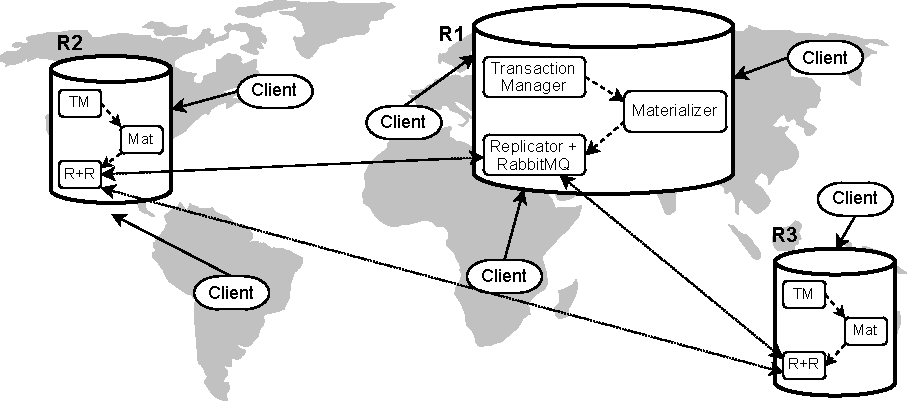
\includegraphics[width=0.8\linewidth]{PotionDBArch}
	\caption{PotionDB Architecture}
	\vspace{-20pt}
	%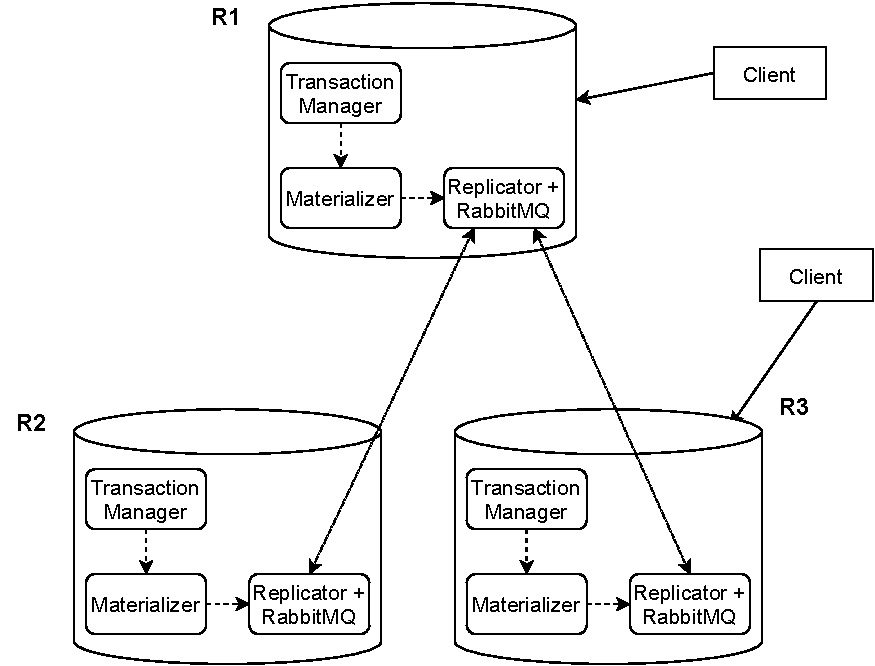
\includegraphics[width=.95\linewidth]{potiondb_architecture}
	%\caption{PotionDB Architecture~\carla{wasted space}}
	\label{fig:arch}
\end{figure}

We designed PotionDB with partial geo-replication in mind.
Thus, we assume PotionDB instances to be spread at different locations across the globe (Figure \ref{fig:arch}).
Each location only replicates a subset of the whole data.
The system administrator has control over where each object is replicated.
This allows to account for data locality to ensure fast access to data, while keeping replication and storage costs controlled.
Objects without locality on their access pattern can be replicated everywhere if desired.
We detail this more in Section~\ref{sec:replication}.

%I think details on how transactions work and guarantees do not belong here. So this is OK (but still needs to be explained somewhere).
Clients communicate with the nearest PotionDB location to ensure low latency.
A client's transactions are locally executed in the PotionDB's location the client is connected to.
Updates are propagated asynchronously to other locations.
If a client's transaction accesses objects not locally replicated, other locations with said objects are contacted and involved in the transaction.
We note this should be an exceptional case, not the norm.
We leave further details for Section \ref{subsec:txnproc}.

The internal architecture of each PotionDB server is inspired by Cure~\cite{cure} and is split into three main components.

First, the Transaction Manager coordinates transactions execution, implementing a transactional protocol (Section \ref{subsec:txnproc}) %which ensures
	ensuring the consistency of reads and updates. %  as well as transactions' atomicity.
	
Second, the  Materializer stores the objects on their latest version, alongside the necessary data to generate previous versions when necessary.
Garbage collection ensures data related with versions that are too old is eventually discarded.
%Garbage collection ensures data to generate versions that are too old is eventually discarded.
	%Garbage collection keeps the amount of metadata in check.
	\nuno{André: o que é que esta última frase quer dizer?}
	%O meu objectivo era mencionar que temos um mecanismo de GC que apaga os dados relacionados com a reconstrução de versões que já não são relevantes (versões muito antigas)
	
Third,  the Replicator ensures that committed transactions are replicated asynchronously to other PotionDB instances.
	It is also responsible for receiving remote transactions and forwarding them to the Transaction Manager for local execution.
	%The replication component is aware of each instances' replication scheme, ensuring each one only receives updates for objects it replicates. 
	Further details are presented in Section~\ref{sec:replication}.



%=========================================================================================
%=========================================================================================
%=========================================================================================
%=========================================================================================



\section{Transaction and replication protocols}
\label{sec:transactions}

This section presents the 
%underlying 
protocols used to maintain the state of objects
and execute transactions with TCC in PotionDB. The transaction processing and replication
algorithms are an adaptation of Cure protocols~\cite{cure} to partial replication.
%setting. 
%Next, we show how PotionDB's mechanisms are used to maintain
%the state of materialized views.

\subsection{Objects}
\label{sec:tx:objs}

PotionDB stores two types of CRDTs: common CRDTs~\cite{crdt} and non-uniform CRDTs (NuCRDTs)~\cite{Cabrita17Nonuniform}.
%We now explain the guarantees and uses of each type of objects.

\noindent
\textbf{CRDTs.} CRDTs are replicated objects that are guaranteed to converge
after applying the same set of operations. In particular, PotionDB uses operation-based CRDTs,
in which the convergence of replicas is guaranteed if operations are causally applied.
% respecting causality.  
This is the case in PotionDB, as a valid transaction serialization must respect the happens-before
relation.
%, i.e., the causal order.

Our prototype supports the following CRDTs: last-writer-wins register, for storing opaque values;
add-wins set, for keeping a set where adding an elements wins over a concurrent removal of that element;
add-wins map, for maintaining a map of values;
counter, for maintaining a number that accepts concurrent increment and decrement operations;
average, for maintaining the average of values added to this object.

\noindent
\textbf{NuCRDTs.} Non-uniform CRDTs~\cite{Cabrita17Nonuniform} are CRDTs that guarantee that in a quiescent state, 
the \emph{observable state} of all replicas is the same. 
Two observable states are defined as equivalent iff, for each possible read operation, the result is equivalent when executed on either state.

Unlike normal CRDTs, in NuCRDTs, during the replication process, it is only necessary to propagate
updates that may affect the observable state. For example, consider a maximum object with a \code{insert(n)} and 
\code{getMax()} operations. An \emph{insert} executed in a replica only needs to be propagated 
to other replicas if the inserted value can be the new maximum. 

NuCRDTs allow to save on both replication, processing and storage costs, as not all updates for a given NuCRDT object need 
to be replicated and applied everywhere.
In PotionDB, we support the following NuCRDTs, previously proposed by Cabrita et. al.~\cite{Cabrita17Nonuniform}: 
\begin{inparaenum}[(i)]
\item maximum and minimum objects, for storing the maximum or minimum of the objects added to the object;
\item top-K,  for storing the K entries with largest values;
\item top-K counter  for storing the K map key, value entries with largest values, where the value
can be updated by issuing increment/decrement operations.
\end{inparaenum}
NuCRDTs can be used directly by applications, but are more commonly used for supporting 
views, as detailed in Section~\ref{sec:views_for_apps}.

\nuno{Dar mais detalhes de como funcionam?}

By not propagating all operations, in some cases, a NuCRDT may temporarily expose an incorrect state.
Consider the maximum NuCRDT.  Each replica keeps only the maximum element and 
the elements that were inserted locally. If the maximum NuCRDT also includes a \code{remove(n)} operation,
and the maximum element is removed in a given replica, the replica might not have the new maximum element,
because it might have been inserted in some other replica.  All replicas of the maximum NuCRDT eventually 
converge to the maximum value, as every replica will propagate the local maximum element after receiving the 
remove operation, guaranteeing that all replicas will receive the new maximum value.

Our work extends the NuCRDTs specifications proposed by Cabrita et. al.~\cite{Cabrita17Nonuniform}
in three ways to make them practical for PotionDB.
First,  a top-K object,  instead of keeping only the value associated with an element,  keeps multiple
attributes for each element, as needed for storing a complete view entry. An application can update
the value used for establishing the top elements using a set operation (in top K) or an increment/decrement 
operation (in a top-K counter).  Other attributes can also be updated (an in a map CRDT).

%\carla{I don't understand the next paragraph!}
%As such, a top-K object consists in a set of CRDT maps (rows) with two special elements - the key of the 
%row and the ordered value used to select the top rows.
%An application can update the ordered value associated with a key by issuing a set value operation in top-K objects
%and increments/decrements in top-K counter objects. Other elements can also be updated, given the key of the
%row, with the operations of the data type.% associated with the row element.
% \andre{In the implementation, a Top-K entry is a key, value and "an array of bytes" (so, not other CRDTs inside the Top-K). Should we change the text to reflect that?}

Second, we extend NuCRDT to include information that allows a replica to know if it might be exposing incorrect results. 
This information consists in the timestamps of transactions that could cause the anomaly - e.g. in our maximum NuCRDT, 
this is the timestamp of the transaction with the \emph{remove} operation that deleted the previous maximum. 
Given this information, and knowing the updates that replicas have seen (which is maintained by PotionDB), 
a replica knows that no anomaly can occur if the operation has been seen by all replicas, 
which would have triggered replicas to send operations relevant for the observable state, if any.
 
Third, we extended NuCRDT specifications to maintain a larger observable state to 
reduce the instances in which a replica may be exposing incorrect results.
 % in practice. 
In our example, the maximum NuCRDT
can maintain the two largest elements. Therefore, if the maximum element
is deleted, replicas still have the new maximum. 
This extension is simple for all NuCRDTs we have defined.% besides the top-K counter. 
%\carla{What is "this" is the above sentence?}

\nuno{explicar como fazer?}


\subsection{Sharding}
\label{subsec:sharding}

PotionDB adopts a sharded model, where objects replicated in a location are 
split into multiple shards. For durability, each shard could be replicated in multiple
servers using some replication protocol \cite{paxos,raft,chainreplication}.

In each server,  a shard has a dedicated thread, adopting an approach used in other
database systems, such as H-store~\cite{h-store}. This avoids using locks when 
accessing objects, simplifying the implementation and avoiding issues 
as lock contention.

\subsection{Metadata}
\label{subsec:metadata}

Let $L_1$, ..., $L_n$ be the set of locations in the system. 
Each location $L_j$ keeps a global vector clock $\mathit{vc}_G$, with one entry for each $L_k \in L_1, ..., L_n$.
This clock represents the latest snapshot available in $L_j$, summarizing the transactions integrated in the snapshot.
Each shard $\mathit{sh}_i$ also keeps a local vector clock $\mathit{vc}_i$.
The local vector clock represents the latest snapshot available in $sh_i$, which may be different 
from $\mathit{vc}_G$.
Any shard can access the server's physical clock, $\mathit{pc}$.

A transaction $t$ has an associated read vector clock, $t\!.\mathit{rc}$,  that represent the snapshot
to be read by the transaction. On commit, a transaction is assigned a commit clock, $t\!.\mathit{ct}$, consisting in a 
pair (timestamp, location identifier).  A transaction with commit clock $(n,r_i)$ is in snapshot $\mathit{vc}_G$ iff
$\mathit{vc}_G[r_i] \geq n$.

Each shard maintains an hybrid logical clock (HLC)~\cite{hlc} used to assign timestamps. An HLC uses the 
physical clock of the computer to generate the next timestamp, unless the physical clock is smaller than a timestamp
previously generated/observed. In this case, it returns the maximum previously observed timestamp plus one. 
This guarantees that timestamps generated are monotonically increasing.
%Different shards may concurrently generate the same timestamp - in this case, the shard's id is used to break the tie.
%In fact, any monotonically increasing clock would suffice for implementing $\mathit{pc}$.

Each shard $\mathit{sh}_i$ also maintains a list of prepared transactions, $\mathit{prep_i}$, and a list of commits on hold, $\mathit{hold}_i$.
%While we leverage on physical clocks for our protocols, the correctness of our protocols is independent of the skew of physical clocks between servers.


\subsection{Transaction processing}
\label{subsec:txnproc}

A client executes a transaction by interactively contacting a PotionDB server.
The transaction execution is coordinated by the Transaction Manager (TM).
%
When the TM receives a \emph{begin} operation, it decides which snapshot the
transaction will access, i.e., the latest snapshot available at the current location,
which is represented by the global vector clock $\mathit{vc}_G$.

When receiving an update operation, the TM asks the Materializer to execute the update in
a private copy of the object for the transaction snapshot. When receiving a read operation, 
the TM asks the Materializer to execute the read operation in the private copy 
of the object - if no update has been executed before in the object, a shared copy with the version 
of the transaction snapshot is used. We represent by $t.WS$ and $t.RS$ the sets of objects updated 
and read in transaction $t$.

When the TM receives a commit, it needs to assign the commit timestamp to the transaction. 
For assigning the commit timestamp, the TM runs a two phase protocol with the shards of the objects
updated in the transaction. 
\andre{shouldn't it be named "two phase commit protocol"?}

In the first phase,  the TM sends a \emph{prepare} message to all shards in $t.WS$.
A shard $\mathit{sh}_i$ replies with a timestamp proposal, $(n,i)$, where $n$ is the timestamp
generated by the shard's local HLC and $i$ is the shard identifier. Additionally, the shard adds the information
about the transaction, including the proposed timestamp, to the list of locally prepared transactions, $prep_i$.

The TM collects the replies and sets the commit timestamp of the transaction,  $t\!.\mathit{ct} = (\mathit{mts}, j)$,
with $\mathit{mts}$ the largest received timestamp, and $j$ the 
location identifier.
A commit message is sent to all shards in $t.WS$ with the commit timestamp.

When receiving a commit message for transaction $t$, a shard proceeds as follows.
First, it checks if the commit can be applied,  by checking that no prepared transaction or commit on hold have a 
smaller timestamp.
If so, updates from $t$ are marked as committed and the shard's local vector clock $\mathit{vc}_i[j]$ is 
updated with $t\!.\mathit{ct}$. 
%From this point, the Materializer of the shard will generate versions of the object that
%include the committed updates.
Otherwise, the commit is queued to be applied later, as other transactions may commit with a lower
$\mathit{ct}$ than $t\!.\mathit{ct}$.
In either case,  the transaction is removed from $\mathit{prep}_i$. If $t$'s proposed value was the lowest, 
then the Materializer verifies if any commit on hold can now be executed.

The client is informed of the commit as soon as all shards in $t.WS$ acknowledge the commit message, even if 
some shards queued the commit. Additionally, the TM sends information to update the global vector clock to
include the timestamp of the committed transaction.
Updating the local entry of the global vector clock with the timestamp of committed transactions immediately
promotes freshness, as new transactions will always use the latest committed snapshot.

However, this raises a problem, as some shards (not involved in the committed transaction) 
may still have transactions to commit with smaller timestamps. 
If a transaction that starts in the most recent snapshot issues a read (or update) operation on object $o$ in a shard that has
pending transactions with smaller timestamps, the operation needs to block if there is a transaction prepared or on hold 
that had modified $o$. 

\noindent
\textbf{Operations on objects not locally replicated.}
%\label{subsec:operationsNonLocal}
This is basically the Cure~\cite{cure} protocol for providing TCC.  
Unlike the setting for which Cure was designed, PotionDB is partially replicated and a transaction 
mayaccess an object $o$
%that is 
not locally replicated.
%, $L_i$. 
Extending Cure to support this case was simple. 

When an operation is executed in an object $o$ that is not locally replicated, 
the shard that should hold $o$ fetches 
a copy of the object from a remote replica. The version of the object 
requested is that
of the transaction snapshot,  $t\!.\mathit{rc}$ ignoring the entry for the current location.
It is important to ignore the current location to guarantee a quick reply. 
Otherwise, as updates are propagated asynchronously, the remote replica would need to wait to
receive all transactions from $L_i$ reflected in the transaction snapshot before returning a copy
of $o$.
After receiving the copy of the object, the shard will apply any updates performed to $o$ at $L_i$. Typically,
there will be no updates, as $L_i$ does not replicate $o$.
After this, the transaction accesses the object as any other locally replicated object. When the transaction commit, 
the updates to the object are propagated in the context of the transaction.

\noindent
\textbf{Reads on NuCRDTs.}
As mentioned, due to the way NuCRDTs work, they may temporarily expose 
incorrect results when an operation $o$ changes the set of relevant operations.  
As explained, PotionDB is able to detect this situation, which is expected to be rare. 
%maintains information for a replica to know if this is the case 
%and
%it is expected to be a rare situation. \andre{Shouldn't we mention again we have mechanisms to make this situation even more rare to happen? (e.g., maintaining a top of double the size.)}
Applications may select two behaviors when they start a transaction.
First, to ignore potential anomalies and immediately execute the read in the local replica.
This guarantees fast replies at the cost of potential anomalies. 
%
Second, to strictly enforce TCC. In this case, the read blocks until the replica gathers 
information that no relevant operation is missing. This requires receiving information from
all replicas that operation $o$ was performed and all additional relevant operations, if any, have been
propagated. This is done in the context of the replication process and explained later.

\noindent
\textbf{Triggers.}
%\label{subsec:triggers}
PotionDB has an after update trigger mechanism that can be associated with 
objects in a given bucket or container.
When a transaction is executed at the initial replica, after an update, the code
of the trigger will run and it may issue reads and updates to the same or to a different object.
These updates are part of the transaction, being committed and propagated to other replicas
as part of the transaction.

Triggers can be used directly by applications, but its primary purpose is to support
incremental view maintenance.%, as detailed in Section~\ref{sec:views_for_apps}.
%In the next section

\subsection{Replication}
\label{sec:replication}

Buckets are the unit of replication in PotionDB.  Each location decides which buckets to replicate.
In our e-commerce example, there is a bucket for 
the customers of each online store.  The container \emph{customers} includes all customer buckets.
The EU customers bucket is  replicated in the EU location and
in one or more additional locations for fault tolerance.

PotionDB adopts an operation-based replication approach, where transaction updates 
are propagated to other replicas. To be more precise, in the context of CRDTs, an update
executed in a CRDT generates an \emph{effects} operation, and it is this effect update that is
propagated and applied in relevant replicas. We start by describing how the replication process
guarantees that transaction updates are propagated to all relevant locations. In the end, 
we discuss the special case of NuCRDTs.

When a transaction commits at a shard, that shard sends its part of the transaction to the replicator.  
Given how transactions are committed at a shard, it is guaranteed a shard sends the transactions
ordered by commit timestamp.
If the shard processes no transaction for some time, it notifies the replicator that there are
no parts of transactions for the shard until the current timestamp, obtained from the shards' HLC.

The replicator processes the parts of transactions received from shards in timestamp order. 
For each transaction, the replicator groups the transactions' updates and repartitions the
updates, one for each updated bucket. The new transaction parts are then queued 
for replication, one part for each bucket, being propagated in order to all other locations that 
replicate the bucket. 
Note that a location has a logical stream of updates not only for all buckets the location replicates,
but also for the buckets that a local transaction has updated an object.

The replicator integrates remote transactions as follows.
A replicator subscribes to the logical streams of updates for the buckets it replicates from all other 
locations. For the logical streams of each location, it processes transaction parts in timestamp order.
For a given timestamp, the replicator groups the parts of the transaction $t$ and verifies if the causal dependencies 
of the transaction are satisfied by checking whether $t.rc \leq \mathit{vc}_G$.
If true, the replicator 
%repartitions the transaction according to
%the local shards and 
forwards the
% transaction 
transaction updates to the local shards for execution. 
After all shards involved in a transaction $t$ end, 
%that they have executed their part of the transaction,  
the global
vector clock is updated to include the timestamp of $t$. If false, then some transactions
from other locations need to be applied before executing $t$. So, the replicator continues by processing
the logical streams from other locations.
Furthermore, the replicator piggybacks to other locations the information about locally executed transactions.
For fault-tolerance, a location forwards updates from a failed
location to other locations.

\textbf{Support for NuCRDTs.}
\label{subsec:nonuniform}
%Note: we do not really guarantee causality when considering non-uniform CRDTs. How should we handle this? Do we mention this in the paper? Or maybe mention how we could "fix" this?
NuCRDTs use a non-uniform replication approach~\cite{Cabrita17Nonuniform}, in which some 
updates might not need to be propagated, as explained in Section~\ref{sec:tx:objs}.
Not immediately propagating some updates is straightforward, as, when executed locally, 
an update operation may produce a null \emph{effect} update if there is no
effect in the observable state.

%as update operations generate 
%the \emph{effect} update to be remotely propagated,
%% to other replicas,
%If an update operation has no
%effect in the observable object state, hence does not need to be propagated, 
%the update operation just generates a null effect.

In NuCRDTs, the execution of an operation $o$ may make a previous operation  $o_{p}$
relevant, requiring this previous operation to be propagated to other replicas  
(e.g.  \code{remove(n)} operation in the maximum NuCRDTs makes the insertion of the second
maximum element relevant). There are two cases to be considered.
%
The first case is when operation $o$ is executed initially. Then the effect of
$o$ will include also the effect of $o_{p}$. Thus, as the combined effects are propagated and applied in 
the context of the same transaction, no anomaly is generated.
%
The second case happens when the now relevant $o_{p}$ operation was executed in  
another replica.  This is handled by replication process as follows.  When a location receives
the replication stream from other replicas, it executes the received \emph{effects} in the objects' local copy.
For NuCRDTs, the execution of an \emph{effect} operation may generate additional 
\emph{effects} - in our example, the execution of the \emph{effect}s of $o$ would generate
the effects of $o_{p}$. These extra effects are remotely propagated 
%to other locations 
along with the 
information that a given operation has been executed in the current location. 

\section{Views and Experience}
\label{sec:views_for_apps}

In this section, we discuss how materialized views are supported in PotionDB, by using PotionDB
objects and triggers generated from the view specification. We also discuss
our experience in defining views for the queries of the TPC-H benchmark~\cite{tpch}. 

\subsection{Generated objects and triggers}
\label{subsec:generated_view}

We now outline how PotionDB, given a view specification, generates the 
%right 
objects to hold the view's data and its updates. % the views.
%For the sake of brevity and simplicity, we do not dive deep into the details of the algorithm, instead showing the intuition behind it.

\noindent
\textbf{Generated objects:}
The object used for storing the view's data depends on the type of query being performed. 
%If the query has no  \emph{limit} clause and includes either no aggregation or an aggregation of type sum (or similar, such as count or average), the view will be stored in a map CRDT, where the full materialized view is maintained. 
%If the query has a  \emph{limit} clause or includes an aggregation of type maximum (or minimum),
%the top-K is used.
%If the query has a  \emph{limit} clause and an aggregation of type sum (or similar, such as count or average),
%the top-K counter is used.
If the query has no  \emph{limit} clause and includes either no aggregation or an aggregation of type sum (or similar, such as count or average), maximum or minimum, the view will be stored in a map CRDT, where the full materialized view is maintained. 
If the query has a  \emph{limit} clause and no aggregation, or an aggregation of type maximum (or minimum), the top-K is used.
If the query has a \emph{limit} clause and an aggregation of type sum (or similar, such as count or average), the top-K counter is used.
In any case, the elements of the view are maps with multiple columns, one for each
of the attributes specified in the  \emph{select} of the view definition.  

For a given view definition, one or multiple objects are defined - in the language we defined for 
specifying view,  a view that includes variables will lead to multiple objects,
one for each possible value of the variables. 
In the top sales example presented in Figure~\ref{fig:viewtopsales}, one top-K counter
object is created (as needed) for each month of each year, and its PotionDB key includes
the name of the view plus the month and year.  The top-K counter will have a set
of entries, each one with the identifier of a product and the total sales of the product. The entry
might have additional information, such as the description of the product if that was defined
in the view.

\noindent
\textbf{Generated triggers:}
After determining the objects used to represent the view, PotionDB generates triggers to update 
its contents,
%of the view, 
as base objects are created, updated or deleted.
% (referred simply as updates). 
The trigger will be set for the container (or buckets) specified in the \emph{from} clause of the view
definition.
If a \emph{where} clause is included in the view definition, updates to objects that do not match the 
defined condition will be ignored.

As a view may be composed by multiple objects, it is first necessary to 
determine which view object must be updated. This is achieved from the view definition 
and the values in the update base object - in our running example, 
from the date of a sale, it is immediate to know which view object
must be updated.
Depending on the view and the underlying object used to support the view, the appropriate 
operation on the view object is generated.
This operation consists in applying the same update performed in the base object to the 
corresponding view entry map.
For example, consider the creation of a new sale for a single product $P$, with the value $v_P$. 
In this case, the top-K counter of the month and year of the sale is updated by 
incrementing the total value of sales for $P$ by $v_P$. 
The underlying functionality of the top-K counter guarantees that the updated entries
will be propagated to other replicas when necessary, and that every replica keeps the correct top-K
elements.

\subsection{Developer-defined views}
\label{subsec:programmer_view}

Besides using PotionDB's view language, an application developer can
maintain the data of a view in specific PotionDB objects and define triggers to update
these view objects.

The top-K and top-K counter NuCRDTs include the logic for replicating only the necessary 
updates to maintain in all replicas the top elements for data that is updated using set value 
or increment operations.
When the view does not consist in the topmost elements, the Map CRDT can be used.  
Aggregations defined in the views - e.g. sum, maximum - are supported by using CRDT and NuCRDT 
objects, such as the counter CRDT and maximum NuCRDT.
After defining the objects to be used, the application should define the triggers that (populate and) 
update the view objects. 


%Recall the view specification in Figure \ref{fig:q18_view}.
%\emph{Limit} tells PotionDB that the view's data will be represented by a TopK or TopSum.
%\emph{Order By} specifies how the top's elements will be sorted - first by totalprice, then orderdate.
%These elements will be the "value" of each entry. %Our TopK/TopSum implementation only supports ints - the secondary sorting by orderdate would have to be external.
%The id of each entry will be composed by the elements in \emph{select} not used in \emph{order by}. %NOTE: I can change this if we want to use a clause or similar like ID() just for TopK/TopSum
%After analysing \emph{select}, PotionDB concludes that a TopK can be used given none of the fields in \emph{select} is a SUM or COUNT, thus the increments or decrements provided by TopSum are unnecessary. 
%%Criteria for TopSum vs TopK: at least one of the values of the entry being a SUM/COUNT
%\emph{Group by} tells PotionDB to use one TopK per possible value of QUANTITY.
%In views with two \emph{Group by}, it is the second one that PotionDB uses to decide how many objects it needs to build the complete view. %I think this is poorly explained - basically our grouping (e.g. tops of each month) is done by the 2nd Group By when two Group Bys are present - we don't actually have a use for the first Group By...
%
%%Often, the same kind of query may be instantiated with different values
%Q18 may be instantiated with values of QUANTITY in the range [312..315].
%In practice, this represents different variations of the same type of query - PotionDB must support all these variations efficiently without expensive filtering or processing.
%PotionDB achieves this by deploying a TopK object per possible value of QUANTITY - each object's key will be the concatenation of "Q18" with the value of QUANTITY.
%Executing the right variation of Q18 is as simple as building the key and executing a single read in the database.
%
%%When having multiple fields in the GROUP_BY, PotionDB will deploy a CRDT per possible value of the pair. Note that relational databases would need to do something similar too (one materialized view per possible value)... in practice, we're not supporting one query, but many.
%
%%An alternative solution to concatenating the keys is to use a Map CRDTs, one per field in GROUP BY, and embed them in each other, with the final "level" being the actual view objects (e.g., top). The idea is kinda like "levels of filtering". Should we describe this solution instead? Advantages: easier because only one key for the view, defined by the user. Disadvantages: can't do internal sharding because everything is condensed into a single big object.
%
%Given the information above, PotionDB decides to support Q18’s materialized view with a TopK CRDT per value of QUANTITY - i.e., 4 TopKs.
%Each CRDT is only initialized when the first update for it is issued.
%This means that, for fields in \emph{Group by} that come directly from the base objects, or for parameters that are compared with equality (=) to a field of a base object, it is not necessary to define the set of possible values. %e.g., in the old query Q3, we don't need to define the values of SEGMENT because we define SEGMENT = customer.segment
%That is, we support parameters whose set of possible values is unknown and remain efficient by only initializing view objects as necessary.
%%The phrase above is probably not very clear. What I mean to say is:
%%If on the GROUP_BY we use directly a value of an object (e.g., customer's region) - no need to define the set of possible values
%%If on the GROUP_BY we use a parameter but said parameter is compared directly with equality (i.e., =) to a value of an object (e.g., parameter REGION) - also no need to define the set of possible values
%%If on the GROUP_BY we use a parameter but said parameter is compared with inequality (<, >, <=, >=, !=) to some value of an object (e.g., QUANTITY), we must define the set of possible values - as otherwise, everything could be possible!!! E.g., if we say totalquantity >= QUANTITY, there is a non-finite amount of values of QUANTITY for which this condition is true for every object (e.g., every negative value).
%
%\subsection{Generating updates}
%\label{subsec:generated_updates}
%%NOTE: Important limitation of our algorithm for this view API - we do not support a view based on another view, unless it is a map!!!
%
%After determining the view objects used to represent the view, PotionDB generates two triggers that will be used to update those view objects.
%One trigger corresponds to new/updates of objects relevant to the view (base objects), while the other to removals of said objects.	%Is this safe to say? I don't know how updates would do actually. TPC-H doesn't define updates, only news.
%The respective trigger is fired when a base object is added/updated/removed, generating the necessary updates for the view.
%These updates are then appended to the current transaction, ensuring views get updated simultaneously with the respective base objects.
%The set of base objects of a view is determined by the \emph{from} clause - only objects with the container specified activate the triggers.
%The conditions in the \emph{where} clause further restrict which objects generate updates for the view.
%
%
%
%For the generation of the triggers themselves, for brevity sake, we only present the intuition behind update generation and not the full algorithm.
%For the rest of the explanation, assume \emph{view} refers to all possible variants generated by the parameters, while \emph{subview} refers to one of the variants.
%Assuming the objects in the container are maps, PotionDB uses the field names in \emph{select}, \emph{where} and \emph{order by} as the map's keys to obtain the necessary values.
%
%Fields in \emph{group by} or fields which are compared to parameters in \emph{group by} are used to build the key for the subview to be updated.
%If the field is used directly, or compared as equality, only a single subview is updated. 
%If compared with inequality, the update is issued for all keys of subviews for which the \emph{where} clause is true. %By inequality I mean, <, >, <=, >= and !=.
%Testing $=, <, >, \leq, \geq$ and $\neq$ between two fields or between a field and some constant value is straightforward. 
%Comparing with a parameter is done as follows.
%If comparing by equality and no restriction is defined for the parameter (e.g. parameter REGION compared to customer's region), the field's value is directly used to build the update's key.
%Otherwise, if a restriction is defined, it is verified if the value respects said restriction.
%When comparing by inequality (e.g. QUANTITY), the condition must be tested for every possible value of the parameter - thus, when \emph{where} has an inequality with a parameter, bounds must be defined for the parameter.
%
%Since the objects used to represent a view are known, knowing which type of update to generate is straightforward.
%The matching of fields in \emph{select} with the view is also straightforward - this was already necessary to do previously to determine the required CRDT(s) to represent the view.
%In the example of Figure \ref{fig:q18_view}, it is known that a new order corresponds to an insert to the TopK, while deleting an order would correspond to removing its entry from the TopK.
%An update of totalquantity could imply removes and/or inserts - this can be determined by checking the old value of totalquantity, its new value and to which tops the order should now belong, if any.
%Updates to other fields in select will imply removing the old entry and adding a new entry. %Personally I think better comment the previous two phrases.
%
%PotionDB knows it needs to issue TopK operations, as it has previously determined the view is a TopK.
%Furthermore, it knows which fields of the object are needed and which ones correspond to the TopK's key and the entries' id and value, as this was all determined previously while deciding how to build the view.
%
%
%%\subsection{Specifying views}
%%\label{subsec:views_for_queries}
%%
%%%Should we make it clear somewhere our PotionDB prototype does not have this specification implemented/supported?
%%Given a recurrent query, the application developer can specify one or more views that hold the necessary data 
%%to answer the query directly, without requiring to read multiple objects, do joins or other resource-consuming processing.
%%
%%As in relational databases, the challenge is, thus, to specify the right views for the application's queries.
%%PotionDB's view API (Section \ref{subsec:viewAPI}) and its similarities with SQL make this challenge somewhat similar to the one faced when using relational databases.
%%PotionDB automatically generates the necessary objects and update rules for the view(s), ensuring views are correctly updated when any base object is inserted/updated/deleted.
%%Such inference takes out a considerable burden from the application developer.
%%
%%We now illustrate how to obtain a materialized view’s specification for a given query. 
%%Consider query 3 (Q3) of TPC-H, defined in Figure \ref{fig:q3}
%%\footnote{For simplicity of the example, we assume data is not normalized. Thus, some fields from customer and order tables are assumed to be available on lineitem.}:
%%	
%%\begin{figure}[h]
%%	\begin{lstlisting}[language=SQL]
%%	SELECT o_orderkey, sum(l_price*(1-l_discount)) AS renevue, o_orderdate, o_shippriority
%%	FROM customer, orders,lineitem,
%%	WHERE c_mktsegment $=$ [SEGMENT] and c_custkey $=$ o_custkey and o_orderkey $=$ l_orderkey and o_orderdate $<$ [DATE] and l_shipdate $>$ [DATE]
%%	GROUP BY l_orderkey, o_orderdate, o_shippriority
%%	ORDER BY revenue DESC, o_orderdate
%%	LIMIT 10
%%	\end{lstlisting}
%%\caption{SQL of TPC-H's Query 3.}
%%\label{fig:q3}
%%\end{figure}
%%
%%%\begin{figure}[h]
%%%	Return the first 10 rows: \\
%%%	SELECT l.orderkey, sum(l.price*(1-l.discount)) AS renevue, \\
%%%	\hphantom{SELECT }o.orderdate, o.shippriority \\
%%%	FROM lineitem, orders, customer \\
%%%	WHERE c.mktsegment = [SEGMENT] and c.custkey = o.custkey and l.orderkey = o.orderkey and o_orderdate < [DATE] and l_shipdate > [DATE]\\
%%%	GROUP BY l_orderkey, o_orderdate, o_shippriority
%%%	ORDER BY revenue DESC, o_orderdate \\
%%%\end{figure}
%%
%%The idea behind Q3 is to detect orders of high value for a certain market segment that haven't been fully shipped as of a given date.
%%The top 10 of such orders is presented, sorted by revenue and using as tiebreaker the orderdate.
%%The query has two parameters - DATE and SEGMENT, where date can only take values between 1995-03-01 and 1995-03-31.
%%
%%For the view, we want to select the same fields as in the query, so that all necessary information is in the view.
%%This avoids having to fetch extra data from other objects, which could imply communication with other servers due to partial replication.
%%The \emph{from} and \emph{order by} clauses are also unchanged. %Do I need to justify this?
%%Since the query only needs to list the top 10 rows, we add a \emph{limit} 10 clause.
%%Furthermore, we need to modify the \emph{where} clause to add restrictions to DATE - this query parameter only varies between 1995-03-01 and 1995-03-31, so we add ``and 1995-03-01 $\leq$ DATE $\leq$ 1995-03-31''.
%%This is necessary so that only lineitem objects whose \emph{where} clause is valid for these ranges are reflected in the view's state.
%%No restriction is needed for SEGMENT, as all values of SEGMENT are to be considered for the view.
%%Finally, the group by cause is not used in PotionDB.
%%
%%The final materialized view can be specified as follows:
%%
%%%\begin{figure}[h]
%%%	\begin{lstlisting}[language=SQL]
%%%CREATE view (Q3, views) AS
%%%SELECT orderkey, sum(price*(1-discount)) AS renevue, orderdate, shippriority
%%%FROM lineitem
%%%GROUP BY orderkey, orderdate, shippriority
%%%
%%%
%%%WHERE mktsegment $=$ [SEGMENT] and orderdate $<$ [DATE] and shipdate $>$ [DATE] and 1995-03-01 $\leq$ DATE $\leq$ 1995-03-31
%%%ORDER BY revenue DESC, orderdate
%%%LIMIT 10
%%%	\end{lstlisting}
%%%\caption{PotionDB specification of a view for TPC-H's Query 3}
%%%\label{fig:q3_view}
%%%\end{figure}
%%
%%\begin{figure}[h]
%%	\begin{lstlisting}[language=SQL]
%%	CREATE VIEW (Q3, views) AS
%%	SELECT Segment, OrderKey, SUM(Price * (1 - DISCOUNT)) AS Revenue, OrderDate, ShipPriority
%%	FROM Lineitem
%%	WHERE orderdate < [DATE] and shipdate > [DATE]
%%	GROUP BY OrderKey, OrderDate, ShipPriority
%%	GROUP BY DATE, Segment
%%	ORDER BY revenue DESC, OrderDate ASC
%%	LIMIT 10
%%	\end{lstlisting}
%%	\caption{PotionDB specification of a view for TPC-H's Query 3}
%%	\label{fig:q3_view}
%%\end{figure}
%%
%%\subsection{Generated view}
%%\label{subsec:generated_view}
%%
%%We now show how PotionDB, given a view specification, generates the right objects to hold the view's data and its updates.
%%For the sake of brevity and simplicity, we do not dive deep into the details of the algorithm, instead showing the intuition behind it.
%%
%%Recall the view specification in Figure \ref{fig:q3_view}.
%%\emph{Limit} tells PotionDB that the view's data will be represented by a TopK or TopSum.
%%\emph{Order By} specifies how the top's elements will be sorted - first by revenue, then orderdate.
%%These elements will be the "value" of each entry.
%%The id of each entry will be composed by the elements in \emph{select} not used in \emph{order by}. %NOTE: I can change this if we want to use a clause or similar like ID() just for TopK/TopSum
%%After analysing select, PotionDB concludes the \emph{revenue} field in \emph{order by} is a sum and, thus, decides to use a TopSum in order to support increments and decrements of an entry.
%%
%%The parameters of the query, [SEGMENT] and [DATE], in practice represent different variations of the query.
%%That is, the query may be instantiated with different values of both SEGMENT and DATE.
%%As such, it is necessary for the materialized view to support all these variations efficiently, without requiring expensive filtering or processing.
%%PotionDB accomplishes this by deploying a different object for each value of a parameter - in this case, a different TopSum CRDT for each pair of SEGMENT, DATE. 
%%The key of each object is the concatenation of “Q3” with the value of SEGMENT, followed by DATE’s. 
%%The order of the parameters in the key is the order of their appearence in \emph{Where}. 
%%Executing the right variation of the query is as simple as building the key and executing a single read in the database.
%%%For this, a different object is used for each pair of SEGMENT, DATE - the key of the view for each object is the concatenation of "Q3", the value of SEGMENT followed by DATE.
%%%The order is the same as the order by which the parameters appear in \emph{Where}.
%%%Executing the right variation of the query is as simple as building the key and doing a direct get on the database.
%% 
%% %There is an alternative solution (which we actually do in our implementation depending on the query) for handling parameters. This different solution consists in using Map CRDTs, one per parameter, and embed them on each other. So the idea is kinda like "levels" of filtering. Should we describe this solution instead? Advantages: easier because only one key for the view, defined by the user. Disadvantages: can't do internal sharding because everything is condensed into a single big object.
%% 
%% Given the information above, PotionDB decides to support Q3’s materialized view with a TopSum CRDT per pair of SEGMENT, DATE.
%% Each pair's CRDT is only initialized when the first respective update is executed, thus it is not necessary to know the possible values of SEGMENT.
%% That is, we support parameters whose set of possible values is unknown and remain efficient by only initializing objects as necessary.
%% 
%% \subsection{Generating updates}
%% \label{subsec:generated_updates}
%% %NOTE: Important limitation of our algorithm for this view API - we do not support a view based on another view, unless it is a map!!!
%% 
%% %Should I explain the algorithm in detail? I think for that I would need to present the pseudo-code or at least some parts of it, like e.g. say which structures are needed to gather information collected by parsing the specification, and how triggers are generated from that.
%%After determining the view objects used to represent the view, PotionDB generates two triggers that will be used to update those view objects.
%%One trigger corresponds to new/updates of objects relevant to the view (base objects), while the other to removals of said objects.	%Is this safe to say? I don't know how updates would do actually.
%%The respective trigger is fired when a base object is added/updated/removed, generating the necessary updates for the view.
%%These updates are then appended to the current transaction, ensuring views get updated simultaneously with the respective base objects.
%%The set of base objects of a view is determined by the \emph{from} clause - only objects with the container specified activate the triggers.
%%The conditions in the \emph{where} clause further restrict which objects generate updates for the view.
%%
%%For the generation of the triggers themselves, for brevity sake we only present the intuition behind update generation and not the full algorithm.
%%For the rest of the explanation, assume \emph{view} refers to all possible variants generated by the parameters, while \emph{subview} refers to one of the variants.
%%Assuming the objects in the container are maps, PotionDB uses the field names in \emph{select}, \emph{where} and \emph{order by} as the map's keys to obtain the necessary values.
%%
%%The fields that are compared to parameters are used to build the key for the subview to be updated - when compared as equality, only a single subview is updated. If inequality, the update is isued for all keys of subviews for which the \emph{where} clause is true. %By inequality I mean, < and >.
%%Testing $=, <, >, \leq, \geq$ and $\neq$ between two fields or between a field and some constant value is straightforward. 
%%Comparing with a parameter is done as follows.
%%If comparing by equality and no restriction is defined for the parameter (e.g. SEGMENT), the field's value is directly used to build the update's key.
%%Otherwise, if a restriction is defined, it is verified if the value respects said restriction (e.g. DATE).
%%When comparing by inequality, the condition must be tested for every possible value of the parameter - thus, when \emph{where} has an inequality with a parameter, bounds must be defined for the parameter.
%%
%%Since the objects used to represent a view are known, knowing which type of update to generate is straightforward.
%%The matching of fields in select with the view is also straightforward - this was already necessary to do previously to determine the required CRDT(s) to represent the view.
%%In the example of Figure \ref{fig:q3_view}, it is known that a new lineitem is an increment to a TopSum, an update an increment or decrement depending on the change, and a remove a decrement.
%%This is known as it was previously determined that the view is represented by a TopSum due to limit and the existence of a sum aggregation.
%%It is also known which fields compose the id and value parts of the TopSum entry, as this was previously defined too.
%%Tables \ref{table:new_lineitems} and \ref{table:view_update} showcase, respectively, the example of two new lineitems and the respective view updates.
%%
%%%%Note: Probably the caption should be of both tables?
%%%\begin{table}
%%%	\small
%%%	%\setlength\tabcolsep{0.1pt}
%%%	\setlength\tabcolsep{5pt}
%%%	\begin{minipage}{0.26\textwidth}
%%%	\begin{tabular}{lcc}
%%%		\multicolumn{1}{c}{}               & Item1                          & Item2                          \\ \hline
%%%		orderkey     & 5         & 5         \\
%%%		partkey      & 20        & 10        \\
%%%		suppkey      & 4         & 3         \\
%%%		linenumber   & 1         & 2         \\
%%%		quantity     & 10        & 1         \\
%%%		orderdate    & 15/03/95  & 15/03/95  \\
%%%		shipdate     & 19/03/95  & 17/03/95  \\
%%%		shippriority & high      & high      \\
%%%		mktsegment   & furniture & furniture \\
%%%		price        & 50        & 100       \\
%%%		discount     & 10        & 0         \\
%%%		...          & ...       & ...       \\ \hline
%%%	\end{tabular}
%%%		\vspace{1em}
%%%		\captionof{table}{New lineitems}
%%%		\label{table:new_lineitems}
%%%	\end{minipage}
%%%	\begin{minipage}{0.2\textwidth}
%%%	\begin{tabular}{lc}
%%%		\multicolumn{2}{c}{furniture, 16/03/95}                            \\ \hline
%%%		orderkey     & 5        \\
%%%		revenue      & 140      \\
%%%		orderdate    & 15/03/95 \\
%%%		shippriority & high     \\ \hline
%%%		{} & {} \vspace*{-0.4em}    \\ 
%%%		\multicolumn{2}{c}{furniture, 17/03/95}                            \\ \hline
%%%		orderkey     & 5        \\
%%%		revenue      & 40       \\
%%%		orderdate    & 15/03/95 \\
%%%		shippriority & high     \\ \hline
%%%		{} & {} \vspace*{-0.4em}    \\
%%%		\multicolumn{2}{c}{furniture, 18/03/95}                            \\ \hline
%%%		orderkey     & 5        \\
%%%		revenue      & 40       \\
%%%		orderdate    & 15/03/95 \\
%%%		shippriority & high    \\ \hline
%%%	\end{tabular}
%%%\vspace{1em}
%%%\captionof{table}{Updated views. Note that none of the other pairs of (SEGMENT, DATE) get updated.}
%%%\label{table:view_update}
%%%	\end{minipage}
%%%\end{table}


\subsection{TPC-H in PotionDB}


\subsubsection{Data model}
\label{subsec:dataset}

We now describe our experience applying our 
%proposed 
model to the queries defined in TPC-H.
TPC-H data is typical of an e-commerce service with tables storing information about customers, suppliers, parts (products), orders, 
countries and regions (continents).
Two extra tables represent associations: partsupply and lineitem represent, respectively, a part provided by a supplier
and a product sold in an order. 

As the dataset includes countries and regions, it is straightforward to define a partial replication strategy. 
For each table that will be partially replicated, we define a bucket for each region and a container including all these buckets.
For tables that are fully replicated, there is a single bucket and container. 
We do the following mapping from tables to buckets: 
\begin{inparaenum}[(i)]
\item Customers, suppliers, nations and regions have 
%a nation or 
region directly
associated with it, which is used to select the bucket to use;
\item Orders are stored in the region of the customer;
\item Partsupplies are stored in the supplier's region;
\item Lineitems are stored in the customer's and supplier's region, as this information is relevant for both.
\item Parts are used across the globe, so they are stored in a single bucket to be fully replicated;
\end{inparaenum}

Each table row is stored as a map CRDT, with the key of the row (e.g. the identifier of a customer or the combination of part key and supplier key for partsupply) used as the key in PotionDB's identifier of the object. 
Each columns is represented as a CRDT - e.g. the counter CRDT is used for numbers that are updated using numeric operations and the
LWW register is used for strings and other numbers.
When useful, we de-normalize the data model (as it is common in key-value stores and document databases). 

\subsubsection{Views}
\label{subsec:views_for_queries}

%%Should we make it clear somewhere our PotionDB prototype does not have this specification implemented/supported?
%Given a recurrent query, the application developer can specify one or more views that hold the necessary data 
%to answer the query directly, without requiring to read multiple objects, do joins or other resource-consuming processing.
%An important aspect to consider, when devising the views, is that some queries have parameters and other don't.
%For example, if the goal is to know top seller product of all times (or in a game the leaderboard of the game), the query 
%will have no parameter and the view will
%be exactly the same as the result of the query. However, if the query to be performed by the application has 
%parameters, the view needs to include all values needed to answer the query with the different possible values. 
%The example of top sales view presented in Section~\ref{subsec:interface} exemplifies this, where the view includes
%the top sales products for each month - an application will query the view to get the information for a given month.
%
%\nuno{Qual o objetivo do próximo examplo - mostrar como fazer? neste exemplo não sei bem como especificar...}
%As in relational databases, the challenge is, thus, to specify the right views for the application's queries.
%PotionDB's view API (Section \ref{subsec:interface}) and its similarities with SQL make this challenge somewhat similar to the one faced when using relational databases.
%PotionDB automatically generates the necessary objects and update rules for the view(s), ensuring views are correctly updated when any base object is inserted/updated/deleted.
%Such inference takes out a considerable burden from the application developer.

We have analyzed how to define views in PotionDB for the 22 queries in TPC-H, with different views using different
underlying CRDTs.
We now describe the lessons learned. In the next section we present the evaluation of how PotionDB performs on supporting
 different types of queries.

\paragraph{De-normalization.} PotionDB is a key-value store and does not directly support advanced database functionality,
such as joins.  To address this issue, we de-normalize the database whenever necessary.  
The view in Figure~\ref{fig:viewtopsales} is an example of such de-normalization, with
the product name (\texttt{prodname}) stored in the sales record, instead of the product identifier.

\begin{figure}[t]
\small{
\begin{lstlisting}[language=SQL]
CREATE VIEW (Q5, views) WITH REGION == 
ANY (SELECT DISTINCT R_name FROM region) AS
SELECT R_Name, N_Name, SUM(ExtendedPrice * (1 - Discount)) AS Revenue
FROM Lineitem
WHERE C_NationKey == S_NationKey AND R_Name == [REGION]
GROUP BY N_Name
ORDER BY Revenue DESC
\end{lstlisting}}
	\vspace{-5pt}
	\caption{Revenue of local suppliers (Q5).}
	\vspace{-10pt}
	\label{fig:viewlocalsupliers}
\end{figure}


% diferentes tipos de dados
\paragraph{Data types.} Different types of view require different support from PotionDB underlying data types.
Figure~\ref{fig:viewlocalsupliers} shows the view to support TPC-H query 5, which computes
for each nation in a given region, the revenue from local suppliers. 
This view can be supported by using for each region a map that stores for each nation the sum of the 
revenue for each \emph{LineItem}. The map of each region is a CRDT map, with the name of the nation mapping
directly to a CRDT counter with the revenue for that nation. When a new \emph{LineItem} is added (or deleted), 
the corresponding counter is updated. All replicas will have all the values for all nations.

This contrast with the top sales shown in Figure~\ref{fig:viewtopsales}, that uses a
top-K counter NuCRDT. In this case, whenever a new sale is inserted, the counters associated with the products are
updated, but each replica maintains only a partial view of the top-K object - as explained before, replicas only propagate 
%to all replicas 
the updates for elements that may belong to the top-K.

Finally,  some views are supported by top-K objects. Figure~\ref{fig:q18_view} shows the view to 
support TPC-H query 18, which can be used to return the top 100 most valuable orders larger than 
some given quantity.  In this case, a top-K object is sufficient - the difference with a top-K counter is that,
while in the top-K an entry in the view is completely defined by the value of an order and can be derived 
from the insert (or update) of an order, in the top-K counter, the value of an entry is the result of an 
aggregation over multiple values (in the previous example, \texttt{LineItem}s).


\begin{figure}[h]
	\begin{lstlisting}[language=SQL]
CREATE VIEW (Q18, views) WITH QUANTITY == [312..315] AS
SELECT CustName, CustKey, OrderKey, OrderDate, TotalPrice, TotalQuantity
FROM Orders
WHERE TotalQuantity > [QUANTITY]
ORDER BY TotalPrice DESC, OrderDate ASC
LIMIT 100
	\end{lstlisting}
	\vspace{-5pt}
	\caption{Large volume customer query (Q18).}
	\vspace{-5pt}
	\label{fig:q18_view}
\end{figure}


% definição de variáveis
\paragraph{Variables:} As introduced in Section~\ref{subsec:interface}, it is possible to define 
variables in the specification of views. In some cases, it is important that the view includes information 
for every possible value of the variables - in this case, a different object if maintained for each
value of the variable (or combination of values of multiple variables). 
For example, for the view presented in Figure~\ref{fig:viewlocalsupliers}, there
will be a database object for each region and for the view presented in Figure~\ref{fig:viewtopsales}, there 
will be a database object for each combination of month and year.

In other cases, the application will only query the database using some specific values of the
variables. For example,  the specification of the TPC-H query 18 states that quantity will be instantiated with values
from 312 to 315. In general, it is common for application interfaces to limit the queries a user can perform, 
leading to a similar situation - e.g. hotel reservation applications allow users to check hotels with an average 
rating larger than some predefined values.
Figure~\ref{fig:q18_view} shows how this can be specified in PotionDB for TPC-H query 18. 
In this case, four objects will be created, one for each value of \texttt{quantity}. Whenever a new
order is inserted (or updated), the four objects are updated.

% limitações
\paragraph{Limitations.} The language for specifying views in PotionDB has several limitations, when
compared with support for defining views in relational databases. The main limitations concern the 
lack of support for joins and sub-queries, and the limited expressiveness in clauses like select and where. 
This makes more difficult the specification of views for some complex queries and might even make it 
impossible to use our view definition language.  In this latter case, the programmer can resort to \emph{manually}
define a view, by selecting the appropriate objects to store the information and defining the necessary triggers
to update these objects.

\vspace{-5pt}
\begin{figure}[h]
	\begin{lstlisting}[language=SQL]
CREATE VIEW (Q11_p1, views) WITH NATION == ANY 
(SELECT DISTINCT N_Name FROM nation) AS
SELECT N_Name, Partkey, SUM(Supplycost * Availqty) AS Value
FROM Partsupp
WHERE N_Name == [NATION]
GROUP BY Partkey
LIMIT 1000

CREATE VIEW (Q11_p2, views) WITH NATION == ANY
(SELECT DISTINCT N_Name FROM nation)  AS
SELECT N_Name, SUM(Supplycost * Availqty) AS Value
FROM Partsupp
WHERE N_Name == [NATION]
\end{lstlisting}
\vspace{-2pt}
	\caption{Important stock identification query (Q11).}
	\vspace{-5pt}
	\label{fig:q5_view}
\end{figure}

In general, it is possible to circumvent the limitations by defining additional views.
For example, TPC-H query 11 finds the suppliers stocks in a given nation that represent a significant percentage of the total
value of available parts in the nation. In the TPC-H specification, this 
is computed using a having clause with a condition expressed as a subquery.
In PotionDB, it is necessary to specify two views, as presented in Figure~\ref{fig:q5_view}.
The \texttt{Q11\_p2} view maintains the total value for each nation, while the \texttt{Q11\_p1} view
maintains the top parts for each nation. For reaching the result of TPC-H Q11, the application needs
to read the total value for the nation, and use this value for filtering the top parts (as some of these part may not
reach the percentage ratio specified in the query).


\section{Evaluation}
\label{sec:evaluation}

%\begin{itemize}
%	\item Say that we evaluate PotionDB's performance
%	\item Give a short summary of what we try to access
%	\item Describe the three modes of PotionDB (normal, "partitioned views/Local PotionDB", "single view server/Single PotionDB")
%\end{itemize}


We evaluated PotionDB's prototype, aiming at answering the next questions: 
\begin{enumerate*}[label=(\roman*)]
	\item  \label{enum:q1} Can global views over partially geo-replicated data give better performance than alternative approaches? 	     
	\item \label{enum:q2} Are global views still worthwhile in a single data center scenario?
	\item \label{enum:q3} How do different types of views behave? 
\end{enumerate*}

Our prototype was implemented in Go and uses Google's protobufs to serialize/deserialize all data transmitted.

\subsection{Experimental setup}
\label{subsec:setup}

In our experiments, we compare the following alternative approaches to maintain views:
\begin{itemize}[leftmargin=*,noitemsep,topsep=0pt,parsep=0pt,partopsep=0pt]
	\item \emph{PotionDB}, our proposed approach where all servers replicate the complete materialized view;
	\item \emph{Local}, where each server maintains a local view that includes only the objects replicated in the server - in this case, 
	updates to the view result only from updates to the objects replicated in the server; 
	on reads, it may be necessary to contact multiple servers;
	\item \emph{Global}, where the view is maintained in one server - in this case, a query needs to 
	contact the server that holds the view, if this is not the local server. 
\end{itemize}
The alternative approaches are implemented using PotionDB codebase - in this way, propagation of view updates uses the same underlying mechanisms, but updates are only sent to the appropriate replicas; queries that require access view not locally replicated use the PotionDB mechanism to access objects not locally replicated.  

%We evaluate PotionDB using TPC-H's dataset, queries and updates, as well as with micro-benchmarks.
%For the evaluation using TPC-H, we 
We evaluate PotionDB on Grid'5000's \cite{Grid5000}, using TPC-H's benchmark \cite{tpch}.
We have modeled the database as discussed in Section~\ref{subsec:dataset} and used data generated by the dbgen tool \cite{tpch}.
In our evaluation we selected some queries to define views, trying to consider queries with different requirements. 
For example, while some TPC-H queries concern worldwide data (e.g. query 18 mentioned before), others, \textit{local} queries, concern data of one continent and country (e.g.  queries 5 and 11). The former lead to \textit{global} views, with each entry combining data from all regions, and the latter lead to \textit{local} views, with each entry combining data from a single region.   

In our experiments, we have used 10 machines, with a 2x Intel Xeon Gold 6130 with 192GB of RAM, interconnected with a 10Gbps Ethernet network. 
We have divided the machines in 5 groups,  each one representing a region, with one machine for running the server and one machine for running the clients.  
Data is partitioned as described in Section \ref{subsec:dataset}. 
We have used the Linux \texttt{tc} command to add latency between nodes in different groups, using as reference the latency between AWS instances measured in \cite{AWSLatency} for regions EU (Paris), US (N.Virginia), Canada (Central), Asia (Tokyo) and Middle East (Bahrain). The highest latency is between Tokyo and Paris at 217ms.  This distribution does not include data centers in each continent, as there was no information for Oceania - we note that this is less favorable for PotionDB, as in PotionDB queries are always local, in alternative approaches some queries need to access remote servers. 

For each experiments, we restart the servers and load the initial database. 
Each presented result is the average of three runs. 
For each configuration, we run experiments with an increasing number of clients. 



\subsection{PotionDB performance with geo-replication}

We start by analysing PotionDB's performance in our targeted partially geo-replicated scenario.

\begin{figure}
	\centering
	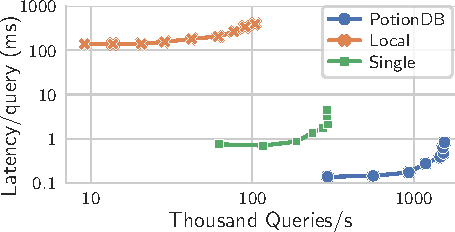
\includegraphics[width=0.6\linewidth]{singleQuery/all_queries_tc}
	\vspace*{-0.75em}
	\caption{Query-only performance of executing all queries.}
	\label{fig:global_local_single_tc}
	\vspace*{-0.9em}
\end{figure}%
\begin{figure}
	\centering
	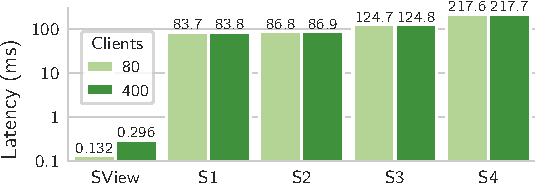
\includegraphics[width=0.72\linewidth]{singleQuery/single_TC_latencies}
	\vspace*{-0.6em}
	\caption{Average latencies of clients in Single PotionDB, depending on the server they are connected to.}
	\label{fig:single_tc_latencies}
	\vspace*{-1em}
\end{figure}%

\noindent
%General query performance and benefits of views
\paragraph{Query performance and benefits of views:}
Figure \ref{fig:global_local_single_tc} shows the results of running all selected TPC-H queries for the three alternative approaches. 
As expected, PotionDB throughput, latency and scalability are considerably better than alternative approaches, reaching 
1.5 million queries/s with latency under 0.6 milliseconds. 
This results from all queries being local, while in alternative approaches, global queries need to access data from 
remote replicas. In this case, servers end up consuming most of the time managing communications with other replicas, leading 
%not only
to higher latency 
%but also to 
and lower throughput. 

When comparing the results of \textit{Single} and \textit{Local}, the \textit{Single} configuration has much lower latency and higher throughput. This is explained by the fact that clients connected directly to the server that holds the views are very fast and 
end up executing a much higher number of requests, that clients in other regions, which experience high latency- this can be 
seen in Figure \ref{fig:single_tc_latencies}, that shows the latency of clients in each region.

To conclude, having global, complete views replicated in every server allows all clients to achieve low latency and high throughput in PotionDB, while \textit{Local} and \textit{Single} approaches suffer from comparatively high latency and low throughput.



\begin{figure}
	\centering
	\begin{subfigure}{.49\linewidth}
		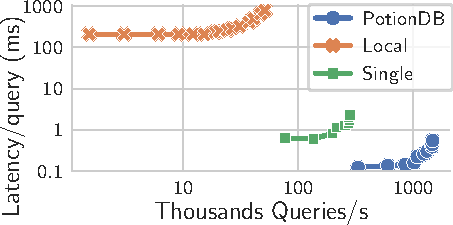
\includegraphics[width=1\linewidth]{singleQuery/q3_latency}
		\caption{Q3-only (global query).}
		\label{fig:q3_tc}
	\end{subfigure}%
	\hspace*{0.2em}
	\begin{subfigure}{.49\linewidth}
		%\raggedright
		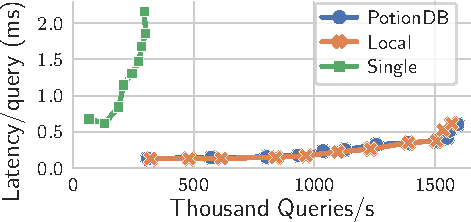
\includegraphics[width=1\linewidth]{singleQuery/q5_latency}
		\caption{Q5-only (local query).}
		\label{fig:q5_tc}
	\end{subfigure}%
	\vspace*{-0.55em}
	\caption{Query performance when executing only Q3 or Q5.}
	\label{fig:q3_q5_tc}
	\vspace*{-1.1em}
\end{figure}

%TODO: Effects of query locality or data locality?
\noindent
\paragraph{Effects of query locality:}
\label{subsec:data_locality}
For better understanding the effects of data locality,  Figures \ref{fig:q3_tc} and \ref{fig:q5_tc} present, respectively, the performance when
executing a single global query (TPC-H Q3) and local query (TPC-H Q5). 
For the global query, the results are similar to the complete workload, the main difference being an increase in latency and reduction in  throughput for the \textit{Local} configuration. In this case this is explained by all queries needing to contact remote servers and results do not include the effects of operations that execute locally.

For the local query, the \textit{Local} configuration performs similarly to \textit{PotionDB}. The reason for this is that, in this case, queries only access the local server that has all necessary information - a client in a region only performs request for data of that region.
In short, PotionDB is efficient for both global and local queries, while \textit{Local} is heavily hindered by latency for any query that is not fully local.

%II have to do these two graphs (I have the necessary data however).
%Here's what those graphs will show.
%
%Graph one: Q3 (global query). PotionDB will scale fine, up to 4.5m ops/s, unnafected by latency (around 0.8ms at 4.5m ops/s). Local PotionDB will be a disaster, with around 210ms latency and up to 70k ops/s. Single PotionDB will get up to around 900k ops/s (1/5th of PotionDB), with around 3-4ms of latency (some effect from added latency).
%
%Graph two: Q5 (local query). PotionDB and Local PotionDB will scale similarly: respectively, 4.1m ops/s and 3.9m ops/s. Both are unaffected by added latency, Local PotionDB even has slightly lower latency. Single PotionDB will have 1/5th of their performance and around 3-4ms latency (i.e., some effect from added latency).
%
%\begin{itemize}
%	\item executing only global queries (Q3) further exacerbates how poorly Local PotionDB performs, due to having to contact all servers for each query. (similar conclusions to the previous section)
%	\item when executing local-only queries (Q5), local PotionDB performs similarly to PotionDB - no redirection of requests is needed (clients only ask for data of their region), thus local PotionDB can efficiently reply to queries with only its local data views. Our solution "does not lose" to the local view solution.
%\end{itemize}

%\begin{figure*}
%	\begin{subfigure}{0.31\linewidth}
%		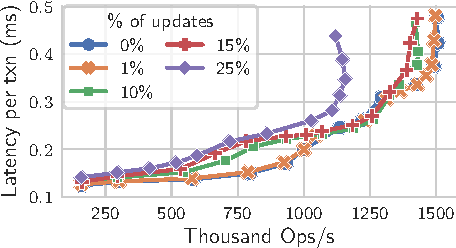
\includegraphics[width=1\linewidth]{singleQuery/upd_rate_global}
%		\caption{PotionDB.}
%		\label{fig:update_rates_global}
%	\end{subfigure}%
%	\hspace*{0.5em}
%	\begin{subfigure}{.31\linewidth}
%		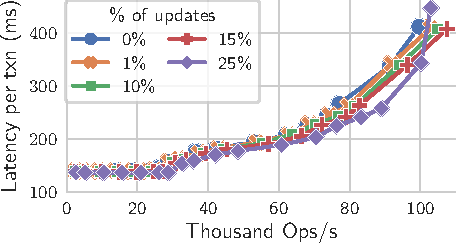
\includegraphics[width=1\linewidth]{singleQuery/upd_rate_local_tc}
%		\caption{Local PotionDB.}
%		\label{fig:update_rates_local_tc}
%	\end{subfigure}%
%	\hspace*{0.5em}
%	\begin{subfigure}{.31\linewidth}
%		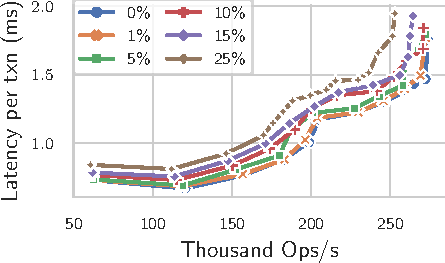
\includegraphics[width=1\linewidth]{singleQuery/upd_rate_single_tc}
%		\caption{Single PotionDB.}
%		\label{fig:update_rates_single_tc}
%	\end{subfigure}%
%	\vspace*{-0.75em}
%	\caption{From left to right, total throughput of PotionDB, Local PotionDB and Single PotionDB with a varying update rate.}
%	\label{fig:upds_tc}
%	\vspace*{-0.6em}
%\end{figure*}
\begin{figure}
	\centering
	\begin{subfigure}{.47\linewidth}
		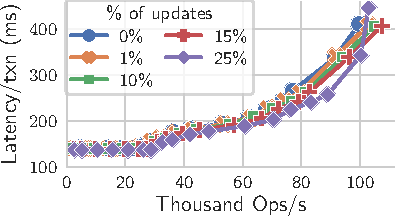
\includegraphics[width=1\linewidth]{singleQuery/upd_rate_local_tc_short}
		\caption{Local configuration.}
		\label{fig:update_rates_local_tc}
	\end{subfigure}%
	\hspace*{0.2em}
	\begin{subfigure}{.52\linewidth}
		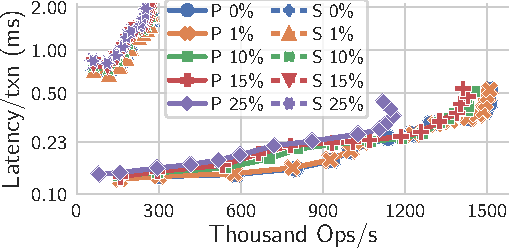
\includegraphics[width=1\linewidth]{singleQuery/upd_rate_tc_global_vs_single}
		\caption{PotionDB and \textit{Single} configurations.}
		\label{fig:update_rates_global_single_tc}
	\end{subfigure}%
	\vspace*{-0.65em}
	\caption{Performance with multiple update rates.}
	\label{fig:upds_tc}
	\vspace*{-1.2em}
\end{figure}


\paragraph{Impact of updates:}
PotionDB approach of maintaining a copy of the views in every server imposes additional load on the system
for keeping view updated,  when compared with the \textit{Local} and \textit{Single} approaches. 
In PotionDB, a view update needs to be executed in every replica while in the other approaches the view update 
is applied only in a single replica. 

To evaluate the impact of updates we consider workloads consisting in different ratios of updates and queries, with
an update being the transaction that creates a new order, and a query being one of the queries defined in
TPC-H - the 25\%/75\% ratio means that 25\% of operations are updates. The results of our experiments
are presented in Figure~\ref{fig:upds_tc}.

%0: 1.511M ops/s, 0.01: 1.517M ops/s,  0.05: 1.46M, 0.1: 1.45M, 0.15: 1.43M, 0.25: 1.157M
%PotionDB has small throughput losses for modest update rates (between 0.1\% and 5.4\% for update rates up to 15\%), while for 25\% it has a significant drop of 23.4\%.
The results show that for PotionDB, for 1\% update rate, the impact in throughput is unnoticeable, when compared with a read-only workload.
The throughput starts decreasing as the ratio of updates increases - 4\% drop for 10\% updates and 23.4\% for 25\% of updates.
The reduction in performance results not only from the fact that view updates need to be executed in all replicas, but also because 
updates are inherently slower as the commit of a transaction require coordination among the multiple shards involved in the transaction. 
Note that queries' latency only raises slightly as, in practice, they seldom need to wait for updates.
%25\%: 0.273304; 0\%: 0.245562
For instance, at PotionDB's maximum throughput for 25\% updates, the query-only latency is 0.273ms, which compares to 0.246ms for 0\% of updates.

%To execute an update transaction, shards have to synchronize to apply the commit protocol (Section \ref{subsec:commit}) - thus, as the update rate gets higher, this synchronization happens more often, potentially making other queries/updates wait.
%This synchronization, as well as multiple updates being in the same transaction, is why update transactions have higher latency than queries, as seen on Figure \ref{fig:update_latency}.
%We note however that in practice queries seldom have to wait for updates unless the server is saturated, as can be seen in Figure \ref{fig:query_latency}.
%The main observable difference in query latency is the latency at the middle of the throughput raising earlier.
%We believe this may be due to network artifacts that lead to latency raising slightly when using over a certain amount of bandwidth - since update transactions have many updates, this threshold is reached with less clients. %TODO: This is... not really a good explanation. Sigh

\textit{Local} throughput improves as the ratio of updates increase.  This stems from the fact that we 
are computing the number of executed operations, and the create transaction includes multiple updates. 
Thus, the overhead for executing a transaction (messages for starting and committing a transaction) is paid
only once for multiple operations\footnote{In PotionDB, if a transaction includes 5 queries/transaction the maximum throughput 
goes to 4.83M op/s (with latency of 0.68ms), when compared with 1.5M ops/s with (with latency of 0.37 ms) for one query per transaction.}.  
Moreover, update transactions do not need to contact other servers - view updates are propagated asynchronously -,  
as 50\% of the orders are local to a region\footnote{This does not occur on the original TPC-H dataset, 
whose orders' items are random. This modification adds locality to orders, which is more realistic for 
an e-commerce scenario and helps \textit{Local} more than PotionDB.} and most other orders
refer few regions.  This leads to a slightly lower average latency \mbox{with higher update rates.}

%fig:update_rates_single_tc
\textit{Single} configuration has throughput losses comparable to PotionDB's, except for 25\% updates where the drop in throughput is smaller 
than PotionDB's due to not having to replicate view updates.
However, even for 25\% updates, \textit{Single}'s throughput is less than 1/4 of PotionDB.

In summary, PotionDB scales well with modest update ratios, which are common in practice.
PotionDB keeps views updated while answering complex global queries in sub-millisecond time.
%Moreover, updates in PotionDB are unaffected by latency between servers.


%Two to three graphs: global with updates, local with updates, (optionally) single with updates. I have to modify the graphs to not count with updates for the views.
%
%Note: both graphs below still account for view updates on their throughput. 
%View updates account for around 2/3rd of the update count.
%
%%Graph global: higher update rates mean lower max throughput and a bit higher latency (e.g., 0\% updates starts at 0.3ms, 100\% starts at 0.5ms). The old graph of this one (still counting with view updates) is on Figure \ref{fig:(new)update_rates}.
%%Graph global: Check Figure \ref{fig:(new)update_rates}
%
%\begin{figure}[h]
%	\centering
%	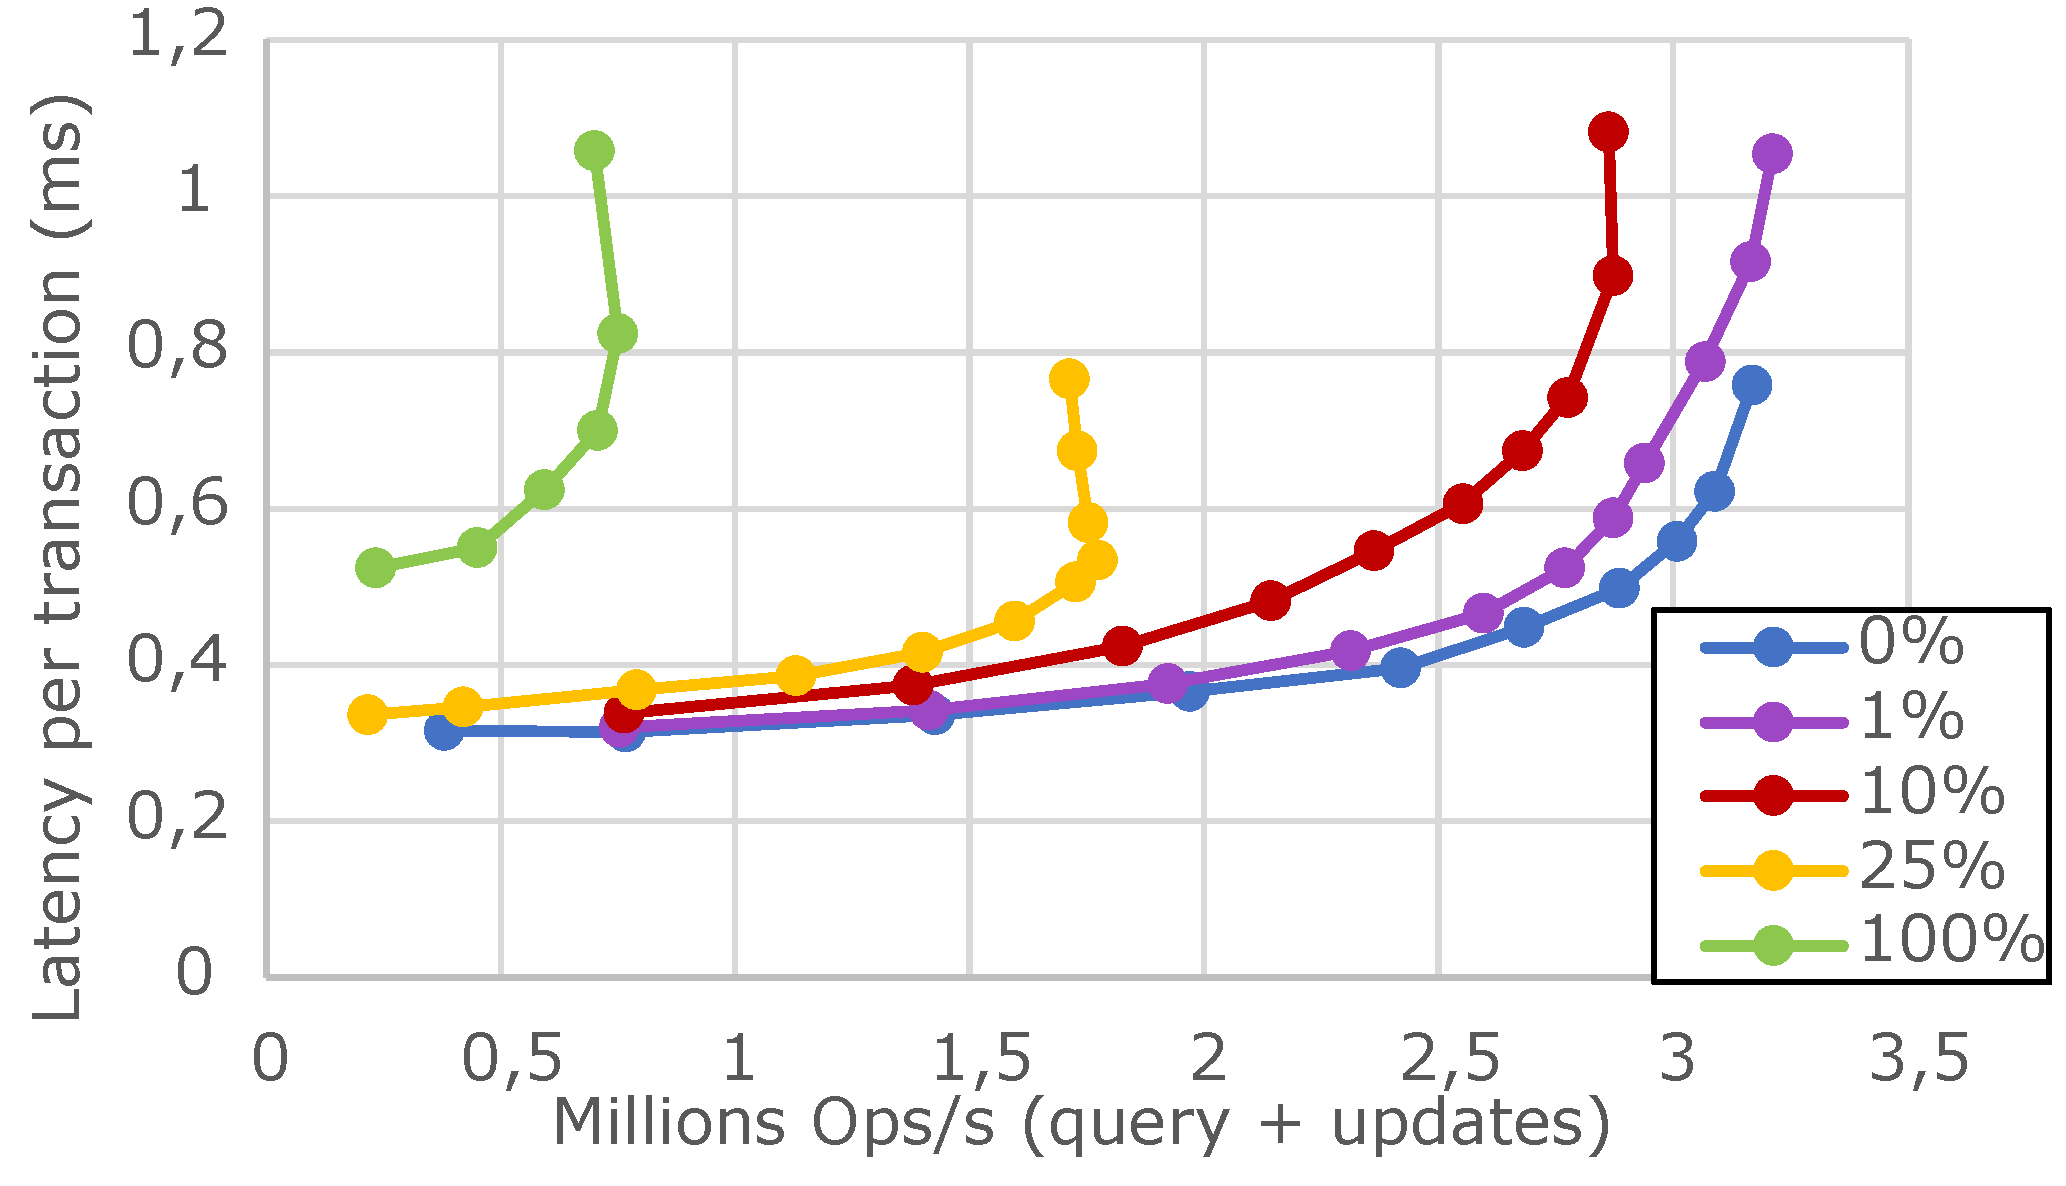
\includegraphics[width=.75\linewidth]{updRate_global_cut}
%	\caption{PotionDB's performance with varying update rate.}
%	\label{fig:(new)update_rates}
%\end{figure}
%
%\begin{figure}[h]
%	\centering
%	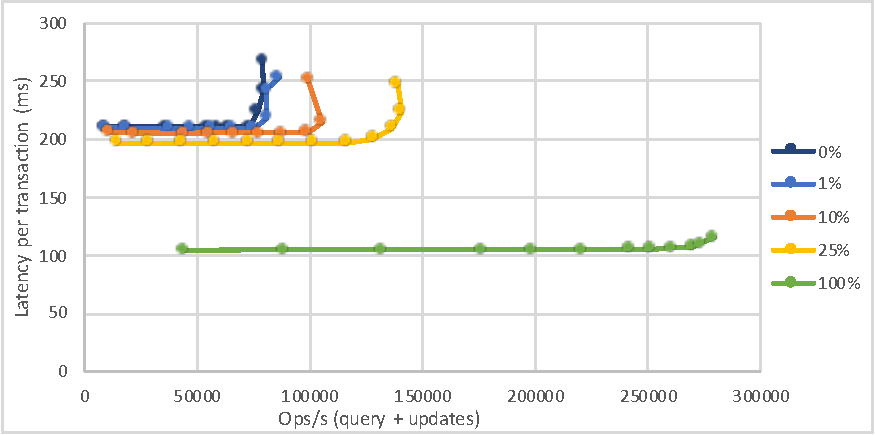
\includegraphics[width=.7\linewidth]{updRate_tc_cut}
%	\caption{Local PotionDB's performance with varying update rate}
%	\label{fig:(new)update_rates_tc}
%\end{figure}
%
%%Graph local: Low max throughput and high latency. Increasing the update ratio decreases latency slightly and increases max throughput con
%
%\begin{itemize}
%	\item Explain what is an update in TPC-H; explain how we do not count with view updates for the throughput;
%	\item Explain why PotionDB is unaffected by the added latency; explain why PotionDB's throughput decreases so heavily. Mention that a lot of the operations are not counted, as there are many view updates.
%	\item Explain why Local PotionDB is affected by the added latency. Explain why Local PotionDB's throughput increases with the higher update ratio and why latency decreases (reason: updates have lower latency than queries because only a subset of the servers need to be contacted, instead of all, so often the highest latency connection can be avoided. Furthermore, updates have more operations per transaction than queries, i.e., more operations per round trip.)
%\end{itemize}

\subsection{PotionDB performance on a single data center}

In this section we study whether keeping global views in all replicas is still an interesting approach when
latency among replicas is smaller, using the extreme case where all servers are in the same data center
(and have no added latency for communication among them).


\begin{figure}
	\centering
	\begin{subfigure}{.49\linewidth}
		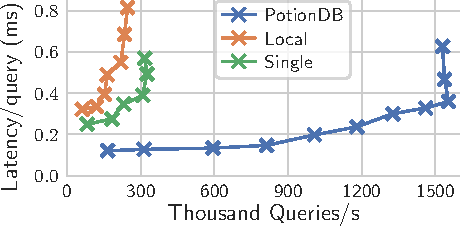
\includegraphics[width=1\linewidth]{singleQuery/all_queries_noTC}
		\caption{All queries}
		\label{fig:all_queries_noTC}
	\end{subfigure}%
	\hspace*{0.2em}
	\begin{subfigure}{.49\linewidth}
		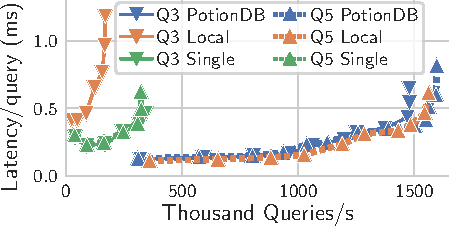
\includegraphics[width=1\linewidth]{singleQuery/q3_q5_noLatency}
		\caption{Single type of query}
		\label{fig:q3_q5_noTC}
	\end{subfigure}%
	\vspace*{-0.65em}
	\caption{Query performance in single DC.}
	\label{fig:global_local_single_noTC}
	\vspace*{-1.2em}
\end{figure}


Figure \ref{fig:global_local_single_noTC} present the results for read-only workloads.
The results for PotionDB are similar to the previous results - this is expected as all operations are local.
\textit{Local} and \emph{Single} have much lower latency and higher throughput when compared with the
geo-distributed setting.  This is expected as the cost of contacting other replicas is much lower now - only the
latency of contacting a node in the same data center.  The maximum throughput is still much lower than that
of \textit{PotionDB}, as the need to contact multiple server for replying to a query induces 
an higher load in the servers. 

For the results with a single query - Figure \ref{fig:q3_q5_noTC} - the trend is similar to 
the results for the geo-replicated setting, but with an increased throughput and lower latency
for \textit{Local} and \textit{Single}, due to the low latency for contacting other replicas. 


\begin{figure}
	\centering
	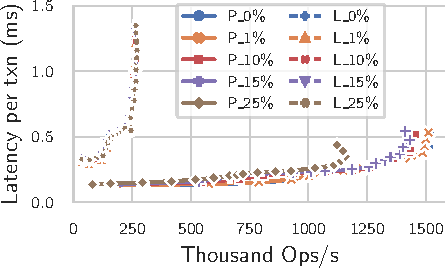
\includegraphics[width=0.62\linewidth]{singleQuery/upd_rate_noTC_global_vs_local}
	\vspace*{-0.65em}
	\caption{PotionDB and \textit{Local} performance with multiple update rates, without added latency.}
	\label{fig:update_rates_global_vs_local_noTC}
	\vspace*{-1.3em}
\end{figure}

%TODO: Would be really nice if I could trim this one further
The results for workloads with updates, presented in Figure~\ref{fig:update_rates_global_vs_local_noTC}, 
show similar trends - PotionDB maintains a significantly better performance than alternative
approaches, which improve throughput and lower latency.  


%similar trends occur with updates, similar conclusions can be taken - Figure \ref{fig:update_rates_global_vs_local_noTC} showcases PotionDB's and Local PotionDB's throughputs for multiple update rates.
%PotionDB's throughput is the same as previously in Figure \ref{fig:update_rates_global_single_tc}.
%%PotionDB is the same as previously observed in Figure \ref{fig:update_rates_global_single_tc}. %, given latency between servers does not affect PotionDB's performance.
%Local PotionDB's throughput only reaches $\sim$250k ops/s for all update rates.
%%For Local PotionDB, the throughput is lower than PotionDB's in all cases, staying at around 250k ops/s for all update rates.
%The stability of Local PotionDB's throughput across different update rates is threefold:
%%Local PotionDB's stable throughput across different update rates is threefold:
%\begin{enumerate*}[label=(\roman*)]
%	\item multiple updates per transaction;%, unlike queries which are one per transaction;
%	\item orders' locality, thus many update transactions are local;
%	%\item orders' locality implies half of update transactions are fully local and most others involve only a subset of servers;
%	\item view updates are not replicated as views are local, which slightly reduces server load. %"do not need to be replicated" instead of "are not replicated"
%	%\item view updates do not need to be replicated unlike in PotionDB as views are local, thus slightly reducing server load.
%	%\item orders' locality implies that half of update transactions can be executed fully locally, with most others only requiring a subset of servers, unlike global queries which require all servers;
%	%\item since views are local, view updates do not need to be replicated and applied in other servers, thus slightly reducing server load.
%\end{enumerate*} %This still has some overlap with the previous section
%Update scenarios favour Local PotionDB, yet its performance is far from PotionDB's.
%%Even though scenarios with updates are favourable for Local PotionDB, it still does not match PotionDB's performance even with an high update ratio.
%Finally, Single PotionDB's thoughput is similar to what was observed in Figure \ref{fig:update_rates_global_single_tc} (and thus lower than PotionDB's), but with lower latencies ranging from 0.24ms to 0.6ms.
%%Finally, Single PotionDB achieves a throughput similar to what was observed previously in Figure \ref{fig:update_rates_single_tc}, but with smaller latencies, ranging from 0.2ms to 0.6ms.
%%Its throughput is, thus, still always lower than PotionDB's.

To conclude, PotionDB's global views provide query throughput and latency unmatched by alternative 
\textit{Local} and \emph{Single} approaches in every tested scenario.
We note, however,  that there is additional memory used for maintaining views in all replicas and this
should be considered when deciding whether to adopt this approach or not in a single data center.


%\subsection{Types of views (or maybe, Views type benchmarking?}
\subsection{Scalability of different types of views}
\label{subsec:microbenchmarks}

Next, we explore how different views behave and scale for different configurations. 
Thus,  we study the behavior of the underlying NuCRDTs supporting different types of 
views: simple limits (Top-K), limits over aggregations (Top-K counter), sum/count (Counter) and average (Average) aggregations.

These experiments were performed using micro-benchmarks, where the underlying NuCRDTs are 
accessed directly by clients - this allows to measure the performance of maintaining the views 
only, without the overhead of storing the base data.
We run the experiments with the same configuration as the previous experiments - 10 machines
divided in 5 groups, with one machine for the server and another for running clients, with no
additional latency added to communications.  
In each experiment, we have 20 CRDTs with random initial data.
Top K and Top K Counter CRDTs are initialized with 10K elements. 
Clients execute transactions consisting in read and updates operations, with each operation 
executed in a CRDT selected randomly using a uniform distribution. For Top K, update operations
are insert and remove of a random elements; for top K counter, update operations are increment 
and decrement to a random element.
Unless stated otherwise, each transaction consists in a batch of 5 operations.


\begin{figure}
	\centering
	\begin{subfigure}{.471\linewidth}
		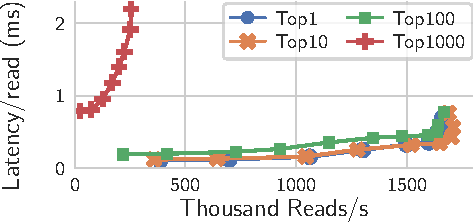
\includegraphics[width=1\linewidth]{singleQuery/bench_top_size_0_upd}
		\caption{1 read per txn.}
		\label{fig:topSize_single}
	\end{subfigure}%
	\hspace*{0.2em}
	\begin{subfigure}{.509\linewidth}
		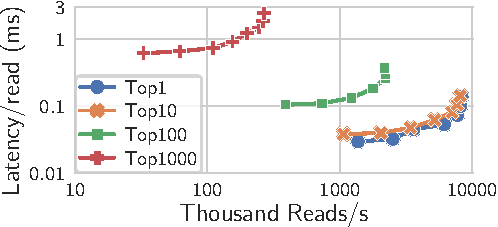
\includegraphics[width=1\linewidth]{singleQuery/bench_top_size_0_upd_5b}
		\caption{5 reads per txn (log scale).}
		\label{fig:topSize_batch}
	\end{subfigure}%
	\vspace*{-0.65em}
	\caption{TopK query performance for multiple top sizes.}
	\label{fig:topSize}
	\vspace*{-0.2em} %TODO: Increase this once we can pull higher the text
\end{figure}

%TODO: Maybe not focus so much on serialization/deserialization: it may not be easy to justify/not the real cause

\paragraph{Scalability of Top-K and Top-K Counter:} %\hspace{0em}
We start by studying the impact of batch size in the number of operations executed. 
Figures \ref{fig:topSize_single} and \ref{fig:topSize_batch} present the results for a read-only workload accessing
top-K objects, where transactions include, respectively, 1 read operation and 5 read operations.
The results show that, for small tops - Top-1 and Top-10, the number of operations executed increases almost
linearly with the number of reads in the transaction.  This shows that in this case,  the fixed overhead of setting 
up a transaction and sending messages dominates the load. 
For larger tops, the number of operations executed increases increasing less. This shows that the amount of data 
transmitted becomes increasingly more relevant in the performance of the system.
We expect that with tops larger than 1000, the number of operations performed when using batches will 
tend to be similar to that when performing read independently.


%The results show that Top1, Top10 and Top100 all perform similarly with 1 read per txn, as communication overhead 
%for small messages (latency, metadata, serialization and deserialization of protobufs) and high number of clients 
%dominate over costs of data transfer and query execution time.
%
%
%
%Grouping reads reduces the aforementioned overhead - with 5 reads per transaction, throughput from Top1 to Top10 drops very slightly ($\sim$2\%), with a much bigger drop for Top10 to Top100 ($\sim$73\%) and Top100 to Top1000 ($\sim$88\%).
%In the latter two cases the amount of data transferred for the replies is the dominating factor, thus making better usage of the network's bandwidth.
%We expect that after 1000, increasing K linearly will decrease throughput linearly as well.
%%by the same factor.


\begin{figure}
	\centering
	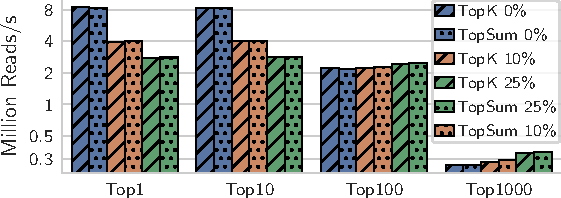
\includegraphics[width=0.76\linewidth]{singleQuery/topk_vs_topsum_5b}
	%\caption{TopK vs TopSum for multiple Top sizes and update ratios}
	\vspace*{-0.6em}
	\caption{TopK vs TopSum for various K and update ratios.}
	\label{fig:topKVSTopSum}
	\vspace*{-0.75em}
\end{figure}

We now compare how Top K and Top K Counter behave for different values of K, with different update
ratios. For updates, we use an add/remove ratio of 90\%/10\%, as it is unusual for an element to be removed
from being considered for a top~\cite{Cabrita17Nonuniform} (note that a top K object keeps information about 
all elements in a partitioned way, with only the top K element being replicated in all replicas). 
Figure \ref{fig:topKVSTopSum} shows that both TopK and Top K Counter maximum throughput is similar, 
showing that the mechanism used for deciding when it is necessary to propagate updates for Top K Counters 
performs well. When considering different update ratios, for small tops, the throughput decreases with an increasing 
ratio of updates, as processing updates is more complex than reads. For larger tops, the throughput with
a larger ratio of updates increases as the overhead of returning the larger tops to clients becomes the dominating 
factor of the performance of the system.


%Thus, we now focus on update scalability.
%%The results with updates are somewhat different to query-only.
%The size of an update is independent of the top's size - thus, as the amount of updates increase and reads decrease, throughput increases considerably for Top1000 and slightly for Top100.
%%Although adding/removing elements gets more expensive as K increases (higher chance for the actual top to be modified), this is offset by the cost of transferring all K elements over the network as a read reply. 
%%TODO: Would be nice to re-add the one above.
%Conversely, Top1 and Top10's throughput decreases as the update ratio goes up, %as commits for updates lock shards, thus reducing read parallelism.
%as commits for updates reduce read parallelism.


\nuno{Interessante, mas sem resultado a comprovar isto pareceria completa especulação.}
%TODO: I would love to leave this here but I feel like I should omit it. Or maybe make it even shorter
\nuno{As a final note, without batching the throughput with updates keeps up better with the query-only scenario.
For instance, Top 10 with 0\% to 25\% updates goes from 8.19M to 2.23M (-72.8\%) and 1.7M to 1.12M (-34.1\%) ops/s for, respectively, 5 and 1 operations per transaction.
Multi-update transactions lock multiple shards instead of just one, so they reduce available parallelism more than single updates do.
}
%The higher drop is because multi-update transactions lock multiple shards instead of only one, thus reducing parallelism for commits and reads.
%As a final note, without batching of neither reads or updates the throughput with updates keeps up better with the query-only scenario.
%Namely, for Top10 with 0\%, 10\% and 25\% updates, with a single operation per transaction, Top10 achieves 1.7M, 1.27M (-25.3\%) and 1.12M (-34.1\%) ops/s, while with 5 operations per transaction it achieves 8.19M, 4M (-51.1\%) and 2.23M (-72.8\%) ops/s.
%This bigger difference is because update transactions with multiple updates can not commit as much in parallel as when only with a single update, as the former has to lock multiple shards instead of just one.


\begin{figure}
	\centering
	\begin{subfigure}{.325\linewidth}
		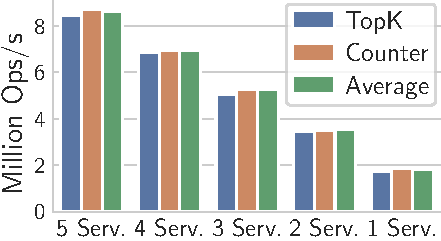
\includegraphics[width=1\linewidth]{singleQuery/n_servers_0_upd_5b}
		\caption{Query-only}
		\label{fig:crdts_0_upd}
	\end{subfigure}%
	\begin{subfigure}{.325\linewidth}
		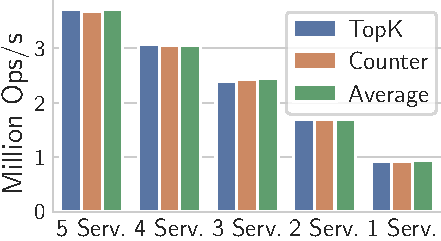
\includegraphics[width=1\linewidth]{singleQuery/n_servers_0_1_upd_5b}
		\caption{10\% updates.}
		\label{fig:crdts_10_upd}
	\end{subfigure}%
	\begin{subfigure}{.34\linewidth}
	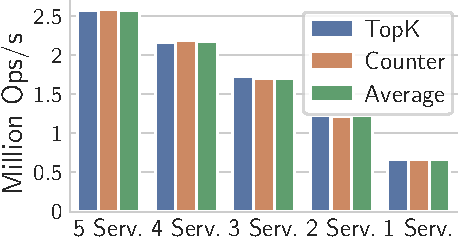
\includegraphics[width=1\linewidth]{singleQuery/n_servers_0_25_upd_5b}
	\caption{25\% updates.}
	\label{fig:crdts_25-upd}
	\end{subfigure}%
	\vspace*{-5pt}
	\caption{Performance of Counter, Average and TopK NuCRDT.}
	\label{fig:crdts:perf}
	\vspace*{-15pt}
\end{figure}

\paragraph{Impact of the number of replicas:}
We now evaluate how NuCRDTs that support views scale with the number of replicas. 
Figure \ref{fig:crdts:perf} shows the throughput of NuCRDTs with different numbers of replicas per NuCRDT 
(for top K,  we used K = 10). 
%Results are presented in Figure~\ref{fig:crdts:perf}. 
The first observation is that, 
for each configuration the performance is similar.  This seems to show that the internal implementation of
the CRDT has little impact in the overall performance of the system, even if internally NuCRDTs are
considerably different.

The second observation is that for read-only workload, the throughput with 5 replicas is almost 5$\times$
the throughput with a single replica - this is expected as operations execute locally in each replica. 
For workloads with updates, the throughput for 25\% updates in a system with 5 replicas being close to 4\% the
throughput of a system with a single replica. This was expected, as updates need to execute in all replicas,
imposing some additional load in all servers.


%%PotionDB scales well both with and without updates.
%With queries only, scalability is near linear on the number of replicas - e.g., Average with 1 server (1S) has 21.2\% of 5S' throughput of 8.62M ops/s.
%With updates, max throughput is smaller and scalability is less linear - e.g., for 25\% updates, Average with 1S has 25.9\% of 5S' throughput of 2.57M ops/s.
%PotionDB's scalability even with updates is solid given each replica applies around 4 times more updates with 5S than with 1S.
%PotionDB's replication mechanism groups remote transactions together, allowing for efficient execution.
%%When executing only queries, throughput scalability is close to linear as reads are locally served - e.g., Average goes from 8.62M ops/s with 5 servers (5S) to 6.92M ops/s with 4S (-19.7\%) and to 1.83M ops/s with 1S (-78.8\%).
%%With updates, max throughput is lower and scales down less linearly, as updates must be propagated and executed in all replicas.
%%E.g., Average with 25\% update rate goes from 2.57M ops/s with 5S to 2.17M ops/s with 4S (-15.6\%) and to 0.665M ops/s with 1S (-74.1\%).
%%However, despite each replica applying around 4 times more updates with 5S than with 1S, the scalability loss is modest.
%%%However, despite the number of updates effectively applied in each server being around 4 times higher with 5 replicas than with 1 replica, the loss on scalability is modest.
%%This is because PotionDB's replication mechanism groups transactions together, allowing for efficient execution.
%%This is because PotionDB's replication mechanism groups updates from different transactions, allowing them to be executed efficiently. %TODO: Maybe add reference to Replication section if I mention this there.







%\newpage
\section{Related Work}
\label{sec:related_work}

%TODO: Veronica uses projection to improve queries, might be worth comparing to.

%Maybe should use only "Consistency" as the paragraph title?
Our work was influenced by works in several different areas.

\noindent
\textbf{Consistency in geo-replication.}
Database systems can be classified as being either strongly or weakly consistent.
Strong consistency systems \cite{spanner, slog, scatter, krikellas2010strongly, megastore, sconekv, lu2021epoch} provide a total order for transactions and are easier to work with.
However, coordination between data centers is required, leading to high latency in geo-distributed scenarios and compromised availability under network partitions \cite{cap}.
By relaxing consistency guarantees, weak consistency systems \cite{dynamo, couchDB, cassandra, chainreaction, cops, riak, eiger} can provide low latency, high throughput and better fault tolerance.
However, concurrency conflicts make those solutions harder to work with.
Casual consistency 
%is a weak consistency model that 
alleviates this problem, however anomalies can still be observed even with cross-object causality \cite{cops, burckhardt2013understanding}.
%Database systems can offer different levels of consistency, and are usually labelled as either strongly or weakly consistent.
%Strong consistency systems \cite{spanner, slog, scatter, krikellas2010strongly, redblue, megastore} are easier to work with as they provide a total order for their transactions.
%Strong consistency requires coordination between data centers, which leads to high latency in geo-distributed scenarios and, as implied by the CAP theorem \cite{cap}, network partitions compromise the system's availability.
%%However, the CAP theorem \cite{cap} implies that network partitions compromise availability.
%%However, the CAP theorem \cite{cap} implies that availability may be compromised in case of network partitions.
%%Furthermore, high latency is to be expected in geo-distributed scenarios as multiple data centers must be contacted for committing a transaction.
%By relaxing the provided consistency guarantees, weak consistency systems \cite{dynamo, couchDB, cassandra, chainreaction, cops, riak, eiger} can provide low latency, high throughput and better fault tolerance.
%However, concurrency conflicts make those solutions harder to work with.
%Causal consistency is a weak consistency model that alleviates this problem, however anomalies can still be observed even with cross-object causality \cite{cops, burckhardt2013understanding}.

\noindent
\textbf{Indexes and views.}
Both indexes and materialized views speed up query execution.
Indexes provide quick access to a table or an object using a non-primary key, and are often used by queries requiring sorting or a given range of values.
Multiple systems implement indexes~\cite{dynamo, couchDB, cassandra, megastore} and there are several proposals on efficient usage and storage of indexes~\cite{lee2020asymmetric, lisa, bindex, slik, abtree, kreachquery}.
%On the other hand, 
%Conversely, 
Materialized views work as a cache for the result of a large query, thus avoiding expensive data recalculations.
However, maintaining views consistent and automatically updated is challenging \cite{oracleViews, chronocache, birds} and few systems implement them \cite{chronocache, marviq, estocada, couchDB, oracleViews, noria}, %even though they can speed up queries considerably.
despite their %considerable 
query speed-up potential and usefulness for analytic queries~\cite{analyticdb, hadad}.
%To the best of our knowledge, 
PotionDB is the first system to support materialized views of global data in a partially geo-replicated scenario.

%The paragraph below does not add anything new compared to the first paragraph. But maybe I could use it as inspiration to shorten the first paragraph
%Geo-distributed scenarios imply high latency when acessing far away data centers, which is required for strong consistency \cite{chronocache, slog, cops, eiger}. 
%Network partitions are also a concern, as they may render strongly consistent systems unavailable.
%Weak consistency can help avoid both problems but lacks the useful consistency guarantees provided by strong consistency.

%\andre{I still need to find citations for partial replication. Any suggestion/starting point is more than welcome}

\noindent
\textbf{Partial replication.}
Partial replication reduces storage costs and can potentially improve a system's performance, as less operations are applied on each server~\cite{sipre, optimisticPartial, coda}, and is thus of interest for geo-distribution.
Careful data partitioning is essential to avoid clients having to contact far away servers, thus experiencing high latency~\cite{sipre, optimisticPartial, coda}.
However, queries over data sharded across data centers is challenging and slow, specially when trying to provide a consistent snapshot.
PotionDB tackles this problem by providing views that summarize partially replicated data and directly answer such queries.

%\noindent
%\textbf{Partial Replication.}
%Partial replication reduces storage costs and can potentially improve a system's performance, e.g., due to less operations being applied on each server~\cite{sipre, optimisticPartial, coda}, and are thus of interest for geo-distribution.
%Data partitioning must be carefully done by considering where each object is relevant, as otherwise clients may need to access far away servers and thus experience high latency~\cite{sipre, optimisticPartial, coda}.
%However, one common problem with partial replication is that, sometimes, it is necessary to query data sharded among different data centers~\cite{sipre}.
%%Many systems provide partial replication \cite{???}.
%%However, a problem not often analyzed in these kind of systems is that some analytic queries may need to consult objects sharded between different data centers.
%Without views, this process can be slow, specially when trying to provide a consistent snapshot of the database.
%PotionDB tackles this problem by providing views that summarize partially replicated data and directly answer such queries.

%I made the CRDT paragraph shorter since we already talk about them in detail in other sections. Maybe should just remove it altogether?

%\noindent
%\textbf{CRDTs.} These replicated data types~ \cite{crdt} guarantee state convergence after applying the same set of operations.
%Thus they are often used in weakly consistent systems, e.g., Redis \cite{redisCRDT} and Riak \cite{riak}.
%Computational CRDTs \cite{computationalCrdt} and non-uniform CRDTs \cite{Cabrita17Nonuniform} are of particular interest for views in PotionDB, as the former summarizes data using aggregations, while the later minimizes the data stored and replicated between replicas while still ensuring queries are answered correctly.
%Maybe add example for Nu-CRDT? (e.g., a top-K CRDT does not need all entries to be replicated)
%\noindent
%\textbf{CRDTs.}
%Conflict-free Replicated Data Types, CRDTs \cite{crdt}, are replicated data types that guarantee state convergence as long as all updates are eventually delivered.
%Thus, they are often used in weakly consistent systems, e.g., Redis \cite{redisCRDT} and Riak \cite{riak}.
%Some types of CRDTs have been introduced that can help with representing views of data, namely computational CRDTs \cite{computationalCrdt} and non-uniform CRDTs \cite{Cabrita17Nonuniform}.
%The former computes some result over data (e.g., a sum), while the later focus on minimizing the information that needs to be replicated to correctly reply to queries (e.g.: a topK CRDT does not need all entries to be replicated).
%In PotionDB every object is a CRDT and, in particular, we leverage on both computational and non-uniform CRDTs to support our views.

\noindent
\textbf{Existing solutions.}
ChronoCache \cite{chronocache} is a middleware caching layer for geo-replicated databases which focus on combining multiple queries into one request and caching query results.
While the caching can speed up future requests, complex queries may still need to contact multiple servers and updates can invalidade the cache or else clients read stale data.

AnalyticDB \cite{analyticdb} focus on optimizing analytic queries. 
It separates write and read paths to prevent complex queries from slowing down writes. 
It also uses indexes to speed up queries. 
However, complex queries still take hundreds of milliseconds to execute and may slow down  simpler queries.
%They do not make usage of views.

%This one is interesting as they leverage on partial replication and data locality to achieve low latency but nothing about views/query speedup.
%SLOG \cite{slog} provides ACID transactions in a geo-replicated scenario.
%By leveraging on partial replication and data locality (as in PotionDB), SLOG achieves low latency on transactions served by a single data center.
%However, queries regarding global data are slow and prone to network partitions.
%PotionDB's global views prevent both issues from happening.

%Not too relevant
%ESTOCADA \cite{estocada} is a system designed to work with polystores and focus on taking advantage of each database's stronger points and make extensive usage of the materialized views provided on each.

Marviq \cite{marviq} tackles the specific situation of efficiently providing a visualization (e.g., scatterplot) of a large data set.
While a very specific scenario, it showcases the need of summarizing large datasets.
Marviq leverages on materialized views for handling range queries.
%While a more specific scenario than the one PotionDB aims for, it showcases similar challenges - large datasets that need to be sumarized and queried efficiently.
%They make usage of materialized views to handle range queries on the datasets.

Magrino et. al. \cite{treaties} propose predictive treaties.
The insight is that some computations can be expressed by treaties, and it is possible to anticipate a range of how a value might change over time.
Compared to PotionDB, treaties use less data than materialized views but can give incorrect query replies, as the range may be inaccurate.
Furthermore, it is unfeasible to predict changes for some data.
Finally, given strong consistency is assumed, queries regarding global data will be slow when synchronization is required and prone to network partitions.
%Magrino et. al. \cite{treaties} propose predictive treaties. 
%The insight is that some computations can be expressed by treaties, and is possible to anticipate a range of how a value might change over time.
%While this can lead to fast query replies and less duplicated data compared to views, since those treaties are not enforced as invariants, it is possible to read incorrect values.
%It may also be unfeasable to predict changes for some data.
%Finally, since a strong consistency scenario is assumed, care is needed to specify treaties in such a way that synchronization is kept to close-by replicas, which may make it difficult or unfeasible to specify treaties concerning global data.

Noria \cite{noria} is a streaming data-flow system.
It leverages on views and partial data to provide fast query reply with reasonable memory usage.
While it features high throughput, it only offers eventual consistency, which complicates application development.
There is also concerns on the performance of queries when a view needs to be rebuilt and data is sharded.

Dynamo \cite{dynamo} and Cassandra \cite{cassandra} are eventually consistent databases.
Both provide indexes to speed up some queries but not materialized views, thus complex queries may need to access large amounts of objects.
CouchDB \cite{couchDB} provides both indexes and materialized views, however views can only refer to data in one partition.

%Should prob make a general comparison to MongoDB/Cassandra/Dynamo

%Comparison to specific solutions?

%Geo-replication, partial-replication

%CRDTs?

%\section{[OLD]Related Work}
%
%Both strongly and weakly consistent solutions exist to support services that require geo replication of their data.
%%Strong consistency solutions like Spanner \cite{???} \comment{likely introduce others}
%%Some examples include, for strong, Spanner \cite{???} and ???; while for weak ??? and ???.
%Strong consistency solutions like Spanner \cite{spanner} and CockroachDB \cite{cockroachdb} provide the ilusion of a single replica, thus making it easier to provide a consistent view for clients.
%However, the CAP theorem \cite{cap} implies that availability may be compromised in case of network partitions, and high latency is expected as multiple data centers need to be contacted for executing operations.
%Weak consistent solutions such as Dynamo \cite{dynamo} and COPS \cite{cops} can provide highly available, low latency operations, but providing a consistent view of the database to clients is challenging.
%Causal consistency is a sub-form of weak consistency that alleviates this problem, however anomalities can still be observed even with cross-object causality \cite{cops, burckhardt2013understanding}.
%
%Systems like Dynamo \cite{dynamo}, COPS \cite{cops} and CockroachDB \cite{cockroachdb} provide geo-replication.
%Dynamo provides partial replication, however reads and updates for multiple keys are done independently, thus there's no causal read of multiple reads.
%COPS provides causal+ consistency and supports transactions for reads, however it doesn't support neither partial replication or views.
%CockroachDB is strongly consistent and, thus, may fail due to network partitions, and does not provide partial replication.
% 
%CRDTs \cite{crdt} are replicated data types that guarantee state convergence, assuming all updates are eventually delivered.
%Thus, they are often used in weakly consistent systems, e.g., Redis \cite{redisCRDT} and Riak \cite{riak}.
%Some types of CRDTs have been introduced that can help with representing views of data, namely computational CRDTs \cite{computationalCrdt} and non-uniform CRDTs \cite{Cabrita17Nonuniform}.
%The former computes some result over data (e.g., a sum), while the later focus on minimizing the information that needs to be replicated to correctly reply to queries (e.g.: a topK CRDT doesn't need all entries to be replicated).
%We leverage on both in our solution.
%
%Alternative solutions to provide global queries on partially replicated data includes using distributed processing systems like Pixida \cite{kloudas2015pixida} or Hourglass \cite{hourglass}.
%However, this impose challenges both consistency-wise, as well as in terms of latency and data transferred.
%The amount of data to be transfered is specially concerning, as if the underlyng systems only provide simple get operations, very high amounts of data may have to be transfered to reply to a small query like a top 10.
%PotionDB avoids this by having materialized views, which allows to have only the required data replicated in every server and thus reply to such query efficiently.
%%COPS doesn't support partial replication
%%Dynamo supports partial replication, but doesn't support views or consistent reads of multiple objects.
%%Start talking about partial replication
%%Mention some geo-distributed DBs, explain that they don't provide partial replication
%%CRDTs, non-uniform replication
%%Maybe at some point refers transactions
%%Refer alternative solution of pixida/parallel jobs.
%%Maybe mention views in consistent databases.
%%Hourglass is mentioned in Pixida paper.

\section{Conclusion}
\label{sec:conclusion}

PotionDB is a weakly consistent, partially geo-replicated database designed to efficiently support
workloads with repetitive queries. 
PotionDB's key feature is the support for materialized views which can be accessed in the context of 
transactions that access both base objects and view objects with  
transactional causal consistency.
These views can be used to efficiently answer recurrent complex queries over data that is partitioned
over different locations, without a single location holding all data.
To support these views, we build on non-uniform CRDTs, extending previous \mbox{proposals to make them practical. }
%PotionDB’s key feature is the provision of efficient and automatically maintained materialized views.
%PotionDB’s views can efficiently answer queries concerning large amounts of global data with a single read operation, even if the base data required to build the view is partitioned across multiple servers.
%Furthermore, PotionDB ensures views and their base data are always consistent by providing transactional causal consistency.

Our evaluation shows that PotionDB can answer complex queries with low latency and high throughput when 
compared with alternative approaches, even under scenarios with considerable update ratios.
%Our implementation and analysis of TPC-H benchmark showcases both the expressivity and efficiency of PotionDB.

%Anything else I should mention? Like the replication/transaction algorithms?

%\begin{acks}
%This work was partially funded by FCT, Fundação para a Ciência e Tecnologia - Portugal, through SAMOA, Project PTDC/CCI-INF/32662/2017, and PhD scolarship SFRH/BD/143401/2019.
%Experiments presented in this paper were carried out using the Grid'5000 testbed, supported by a scientific interest group hosted by INRIA and including CNRS, RENATER and several Universities as well as other organizations (see https://www.grid5000.fr).
%\end{acks}

%This work was supported by the [...] Research Fund of [...] (Number [...]). Additional funding was provided by [...] and [...]. We also thank [...] for contributing [...].


%\clearpage

\balance

%\bibliographystyle{abbrv}
\bibliographystyle{ACM-Reference-Format}
\bibliography{bib}

\end{document}








\section{Transactions}
%\label{sec:transactions}
PotionDB employs a transactional protocol in order to ensure the database's state evolves correctly and that transactions observe casually consistent snapshots.
This is necessary as internally PotionDB is sharded for performance, thus coordination is required.
Furthermore, our transactional protocol is also responsible for ensuring transaction's atomicity, as well as ensure views and their base objects are updated simultaneously and kept consistent.

In this section we describe PotionDB's sharding, our commit and reading protocols as well as how views are kept up-to-date with their base objects. %Do I need to make it clear the transactional protocol is commit + read?


%A table summarizing all symbols could be useful.
%Each PotionDB instance is internally sharded, as described in Section \ref{subsec:sharding}.
%Thus, to enable the provisioning of casually consistent snapshots of the whole database, coordination among partitions is required to execute transactions, ensuring state evolves correctly.
%If no coordination was employed it would be possible to observe inconsistent states of the database - e.g., observe a state where a base object is already updated but its base view is not. %I don't think I need to motivate this further... is it necessary to say this would lead to application errors/difficulties for the application developer, or that it would break transactional causal consistency?

%We define the following notation to help with our protocols definition in this section. %Maybe I should define a table for this like in Cure?
%Let $T$ be the current transaction being considered, $p_T$ the set of partitions for which there is a read or write in $T$, $p_{w(T)}$ the same but for writes only.
%Let $S_1, ..., S_n$ be the set of servers of the system.
%Let $clk^p_i$ be the value of the physical

\subsection{Sharding}
%\label{subsec:sharding}

%Maybe I can mention doing sharding based on some other criteria (e.g., to make better usage of views + objects) is left as future work/orthogonal line of research.

Internally, the Materializer component (our datastore) is sharded.
This allows multicore CPUs to be efficiently utilized,
with reads and updates executing in parallel whenever possible.
Each object $o$ is assigned to only one shard, based on a hash of $o^{\mathit{id}}$.
For clarity, let $o^{\mathit{shard}}$ be the shard where $o$ is stored.
Each shard also has a unique id used for clock disambiguation.
For simplicity, it is also possible to obtain the shard of $o$ from its $id$, or from any read/update operation regarding $o$.

Each shard has one dedicated thread.
This avoids the usage of locks when accessing objects, simplifying the implementation and avoiding other issues such as lock contention.
It also allows for reads and updates on non-overlapping shards to execute in parallel.
In a way, our approach is similar to the one used in H-Store \cite{h-store}.
However, instead of running multiple instances of PotionDB and sharding the data across those instances, we shard the dataset across threads of the same database instance, as this allows for a more efficient communication between shards when necessary.
%Do I need to justify further the H-Store reference? 

%This needs us to define that we access the server with read() and update() before.
%The intuition is that in a given transaction, operations for different shards can execute concurrently without any conflict.
%For multiple transactions, if all transactions are read-only, then there is no conflict either as states do not change.
%However, when considering updates, if there is an overlap of updates of different transactions for the same shard, then there is a conflict, as the results may differ depending on the execution order.
%I am not sure if the "intuition" above is necessary at all.

Ideally, all transactions would execute concurrently at will, and long transactions would also execute concurrently across shards.
However, concurrent writes to the same shard conflict, as the results may different depending on execution order.
Thus, we now define some notations in order to precisely describe the scenarios where operations, i.e. reads and writes, can be executed concurrently.
First, for a given transaction $T$, let $W_T$ and $R_T$ be, respectively, the set of writes/reads present in $T$.
We say that $o \in W_T$ (resp. $o \in R_T$) if there exists a write (resp. read) operation in $W_T$ (resp. $R_T$) for object $o$.
Furthermore, $\mathit{sh}_{W_T}$ (resp. $\mathit{sh}_{R_T}$) returns the set of shards for which at least one object $o$ resides in each shard, i.e., 
$\forall\, s \in \mathit{sh}_{W_T} : \exists o^{\mathit{shard}} \in W_T : \mathit{shard} = s$ (and similarly for $R_T$).

The scenarios where transactions can safely execute concurrently are as follows:

\begin{compactitem}
	\item Subsets of operations of a given transaction $T$ that belong to different shards may always execute concurrently;
	\item For a given set of transactions $T_1$, ..., $T_n$, if all transactions are read-only, they can execute freely in any order, exploiting full concurrency between shards;
	\item For a given set of transactions $T_1$, ..., $T_n$, with a subset of the operations being writes, the transactions can execute concurrently as long as 
	$\forall\, T_a, T_b \in T_1, ..., T_n :T_a \neq T_b \implies (\mathit{sh}_{W_{T_a}} \cap \mathit{sh}_{W_{T_b}} = \emptyset)$ (informally, there is no intersection of shards between any of the write sets). Note that read sets can intersect freely.
\end{compactitem}

In PotionDB, views are defined to answer complex queries directly with a single read.
Due to the nature of hashing, views are likely spread across different shards.
Thus, we expect most transactions will access few shards, allowing transactions to execute concurrently even in the presence of concurrent updates to unrelated objects. Our practical evaluation shows that sharding improves PotionDB's performance considerably.
\andre{TODO: I don't actually have any results that demonstrate this easily. The few experiments I did in this regard do not show a very considerable improvement. Maybe I can just remove this phrase?}

%Other possible solutions to make use of multi-core CPUs are possible, for instance:
%\begin{compactenum}
%	\item \label{item:locks} using locks to protect the same object from being concurrently modified;
%	\item \label{item:multiplePotion} running multiple PotionDB servers in the same computer.
%\end{compactenum}
%
%Alternative \ref{item:locks} is difficult to implement efficiently, as the right level of lock granularity is needed.
%Deadlocking, lock overhead, and fairness are also concerning.
%Our solution does not need to lock data, thus avoiding lock overhead and deadlocks, while also being easier to implement.
%
%Alternative \ref{item:multiplePotion} would imply more replicas running in the system, which increases both replication and storage costs.
%This would also imply concurrency conflicts even in the same computer. \carla{computer or replica?}
%Finally, while this solution can allow more clients to be processed in the same period of time, and is rather easy to implement, it does not improve the performance of each client, as each transaction must be done in a single replica (and thread) to avoid breaking consistency. \andre{Does this need to be explained? The idea here is that we would lose the "write follows reads/writes" property.}

Some existing solutions shard data across multiple machines in a data center \cite{cops, eiger, cure, mdcc, gentlerain}.
While this requires coordination between machines for executing cross-shard transactions (e.g. with 2PC), it allows to scale the dataset size further than what a single machine can handle.
This is, however, orthogonal to our research, as we focus on scalability of each individual server.
%Any need to mention we could adapt this to PotionDB if desired?

\subsection{Clocks}

Let $S_1$, ..., $S_n$ be the set of servers in the system. \carla{$S$ is already used as state, cannot be used as server.}
Each server $S_j$ keeps a global vector clock $\mathit{vc}_G$, with one entry for each $S_k \in S_1, ..., S_n$.
This clock represents the latest snapshot available in $S_j$.
Each shard $\mathit{sh}_i$ also keeps a local vector clock $\mathit{vc}_i$.
The local vector clock symbolises the latest snapshot available in $sh_i$, which may be different from $\mathit{vc}_G$.
Any shard can access the server's physical clock, $\mathit{pc}$.
Each shard $\mathit{sh}_i$ also keeps a list of prepared vector clocks, $prep_i$, as well as a list of commits on hold, $\mathit{hold}_i$.
While we leverage on physical clocks for our protocols, the correctness of our protocols is independent of the skew of physical clocks between servers.
We assume $pc$ to be monotonically increasing when accessed sequentially.
However different shards may concurrently read the same value of $pc$ - in this case, the shard's id is used to break the tie.
%In fact, any monotonically increasing clock would suffice for implementing $\mathit{pc}$.

A transaction $T$ has two clocks associated - a read vector clock, $T\!.\mathit{rc}$, and a commit clock, $T\!.\mathit{ct}$ (single scalar, i.e., a timestamp).
The former represents the snapshot to be read by the transaction, while the latter is the snapshot that will be generated by the transaction's updates on commit.
Applying a local commit only advances $S_j$'s entry in a vector clock, hence why a single scalar is enough for $T\!.\mathit{ct}$.
Updates are only applied when a transaction is committed. 
Reads are applied as soon as they are issued. %This phrase probably belongs in another place.

\subsection{Commit protocol}
\label{subsec:commit}

%Variables:
%txnInfo: txnID -> VectorClk x set(shardID)


\begin{algorithm}
\small{
	\begin{algorithmic}[1]
		\Statex tID, svID,  shID  \Comment{transaction, server, and shard identifiers}
		\Statex OP = $\{$\code{read}, \code{update}$\}$  \Comment{operations}
		\Statex oID = Key$\times$Bucket$\times$Type \Comment{object identifier}
		\Statex \textbf{global}
		\Statex \quad globalVC: VC  \Comment{global vector clock of $S_j$}
		\Statex \quad txInfo: svID $\to$ \textsf{set}$\langle$shID$\rangle$ \Comment{shards written by each server}
		\Statex \quad ongoingTxs: \textsf{set}$\langle$Txs$\rangle$ \Comment{ongoing transactions}
		
		\Function{startTransaction}{clientVC: VC} \label{alg_line:startTransaction}
		\State \textbf{wait until} clientVC $\leq$ globalVC	\label{alg_line:waitClientClk}
		\State readVC $\leftarrow$ globalVC	\label{alg_line:rc}
		\State txId $\leftarrow$ \Call{generateUniqueId}{ }
		\State txInfo[txId] $\leftarrow \emptyset$ 
		\State \textbf{return} txId, readVC
		\EndFunction
		\Function{updateOp}{txId: tID, objId: oID, op: OP}
		\State txInfo[txId] $\leftarrow$ txnInfo[txId] $\cup$ objId$^{\mathit{shard}}$	
		%Maybe on Sharding subsection I should mention we can get the shard of any object, update or read by doing ^{shard} (instead of just saying of any object)
		\State \textbf{send} \Call{update}{txId, objId, op} \textbf{to} objId$^{\mathit{shard}}$
		\EndFunction
		\Function{\textls[-20]{readOp}}{txId: tID, readVC: VC, objId: oID, op: OP} \label{alg_line:readTM}
		\State \textbf{send} \Call{read}{txId, readVC, objId, op} \textbf{to} objId$^{\mathit{shard}}$
		\EndFunction
		\Function{commitTx}{txId: tID, readVC: VC}
		\ForAll{sh \textbf{in} txInfo[txId]	} \Comment{all shards written by txId}
		\State \textbf{send} \Call{prepare}{txId} \textbf{to} sh	\label{alg_line:prepare}
		\EndFor
		\State maxTs = $\bot$	\Comment{initialize timestamp. This will be T.ct}
		\ForAll{sh \textbf{in} txInfo[txId]}	
		%\State suggestedTs $\gets$ \textbf{reply of} sh \textbf{from}  \textsc{prepare}
		\State  \textbf{receive} suggestedTs \textbf{from} sh
		\State maxTs $\leftarrow$ \Call{max}{maxTs, suggestedTs} \label{alg_line:maxTs}
		\EndFor
		\ForAll{sh \textbf{in} txInfo[txId]}	
		\State \textbf{send} \Call{commit}{txId, readVc, maxTs} \textbf{to} sh \label{alg_line:commitSend}
		\EndFor
		\EndFunction
		\LeftComment{An always running routine}
		\Function{globalClockUpdate}{ } \label{alg_line:globalClockUpdate}
		\ForAll{T \textbf{in} ongoingTxs}
		\ForAll{sh \textbf{in} txInfo[T.txId]}
		\State  \textbf{receive} reply \textbf{from} sh
		\EndFor
		\State globalVC[j]  $\leftarrow$ \Call{max}{globalVC[j], T.ct}
		%The max is needed because  two transactions (this one, other) on disjoint partitions could commit concurrently (safe) and the other transaction commit first with a higher ts than this one.
		\State txInfo[T.txId] $\leftarrow$  $\bot$ 
		\EndFor
		\EndFunction
	\end{algorithmic}
	\caption{Transaction manager of S\textsubscript{j}: commit and read protocol}
	\label{alg:commit_tm}
	}
\end{algorithm}

\begin{algorithm}
\small{
	\begin{algorithmic}[1]
		\Statex \textbf{global}
		\Statex \quad vc$_i$: VC \Comment{latest applied clock of sh$_j$}
		\Statex\quad  prep$_i$: \code{heap}$\langle$TS$\rangle$ \Comment{list of (sorted) prepared timestamps}
		\Statex \quad hold$_i$: \code{heap}$\langle$tID$\times$VC$\times$TS$\rangle$ \Comment{commits on hold (txId, rc, ct)} 
		%commits that have been confirmed but not yet applied (due to some timestamp in prepi that is smaller or another timestamp in holdi with a smaller value)
		\Statex \quad txUpds: tID $\to$ \code{list}$\langle$OP$\rangle$ \Comment{Transaction updates}
		%Note: implementation-wise, prepi and holdi are heaps. Is that more appropriate to say than list/queue? The important part for the algorithm is to be sorted by timestamp.
		%IMPORTANT NOTE FOR THE CORRECTNESS OF THE ALGORITHM: I think rremote transactions may affect the correctness of this protocol if we only use a single scalar for the commit timestamp. 
		%More precisely, assume e.g. T1 is about to be prepared on sh1, sh2 and sh3, and T2 is a remote transaction for sh1, sh2. 
		%We could have the prepare of T1 be before T2 is applied on sh1 but after being applied on sh2. 
		%Should we ensure T1 is only committed after T2 is applied in both sh1 and sh2? 
		%Our implementation does that, the algorithm here (and the explanation in the paper) does not. 
		%The change to the algorithm to support that is to make sure the whole vector clock is considered when deciding and applying the commit, instead of only a timestamp.
		%Or maybe all of this doesn't matter because T1 and T2 are supposed to be concurrent anyway.
		\Function{prepare}{txId: tID} \label{alg_line:prepstart}
		\State ts  $\leftarrow$ (pc, j)  \Comment{current physical clock of sh$_j$}
		\State prep$_i$.\Call{sortedAdd}{ts, txId}
		\State \textbf{send} ts \textbf{to} TM 	\label{alg_line:prepfinish} \Comment{reply to transaction manager}
		\EndFunction
		\Function{commit}{txId: tID, rc: VC, ct: TS}
		\State minPrep $\leftarrow$  prep$_i$.\Call{min}{ }.txId
		\State prep$_i$.\Call{remove}{txId}	\label{alg_line:removePrep}
		\If{\Call{canCommit}{txId, ct}} \label{alg_line:call_canCommit}
		\Call{applyCommit}{txId, rc, ct}
		\Else \
		hold$_i$.\Call{sortedAdd}{ct, txId, rc}
		\EndIf
		\LeftComment{if txId was lowest prep$_i$, then lowest commit in $\mathit{hold_i}$ may be applicable}
		\If{minPrep = txId}		
		\State \Call{applyHoldCommits}{ } \label{alg_line:call_checkHold}	%Even if txID’s was put on hold, it may have been the lowest prepare and, thus, another commit on hold may be OK to be applied now
		\EndIf 
		\EndFunction
		\Function{canCommit}{txId: tID, ct: TS} \label{alg_line:start_canCommit}
		
		\If{prep$_i$.\Call{isEmpty}{ } $\wedge$ hold$_i$.\Call{min}{ }.ct $<$ ct $\vee$ \\ 
			\qquad \ prep$_i$.\Call{min}{ }.ts $<$ ct $\vee$ \\ 
			\qquad \  hold$_i$.\Call{notEmpty}{ } $\wedge$ 
				hold$_i$.\Call{min}{ }.ct $<$ ct}
		\State \textbf{return} false
		\EndIf
		\LeftComment{safe to commit, as for all $T$ in prep$_i$ or hold$_i$ T.ts $>$ ct}
		\State \textbf{return} true
		\EndFunction \label{alg_line:finish_canCommit}
		\LeftComment{I don't think we need the pseudo-code for this function.}
		\Function{applyHoldCommits}{}()	\label{alg_line:start_checkHold}
		%Checks if holdi.min() can be applied (i.e., prepi.min() > holdi.min()). If yes, remove txn from holdi, apply, and repeat process. If not, stop. I don’t think we need the pseudo-code of this.
		\If{hold$_i$.\Call{isEmpty}{}()} \textbf{return}
		\EndIf
		\If{prep$_i$.\Call{isEmpty}{ }}
		\While{hold$_i$.\Call{notEmpty}{ }}
		\State txId, rc, ct $\leftarrow$ hold$_i$.\Call{removeMin}{ }
		\State \Call{applyCommit}{txId, rc, ct}
		\EndWhile
		\State \textbf{return}
		\EndIf
		\State minPrep $\leftarrow$ prep$_i$.\Call{min}{ }.ts
		\For{\textbf{all} (txId, rc, ct) \textbf{in} hold$_i$}
		\If{ct $<$ minPrep}
		\State hold$_i$.\Call{removeMin}{ }	\Comment{same as (txId, rc, ct)}
		\State \Call{applyCommit}{txId, rc, ct}
		\Else \ \textbf{return}
		\EndIf
		\EndFor
		\EndFunction	\label{alg_line:finish_checkHold}
		\Function{applyCommit}{txId: tID, rc: VC, ct: TS}
		%Applies the updates. I omitted the details of applying updates as I believe they are unnecessary
		\Statex \hspace*{1.5em} $\cdots$ \Comment{apply updates to the CRDTs}
		\State vc$_i$[j]  $\leftarrow$ ct
		\State txUpds[txId] $\leftarrow$  $\bot$
		\State \textbf{send} reply \textbf{to} TM \label{alg_line:applyCommitReply} 
		\Comment{received by \Call{\textls[-30]{globalClockUpdate}}{}}
		\EndFunction
		\Function{update}{txId: tID, objId: oID, op: OP}
		\State txUpds[txId].\Call{append}{op}
		\EndFunction
		\Function{applyRead}{txId: tID, rc: VC, objId: oID, op: OP}	\label{alg_line:readShard}
		\If{rc $\geq$ objs[objId].\Call{lastVersion}{ }}
		\State \textbf{return} 	objs[objId].\Call{read}{txUpds[txId]}	\label{alg_line:read}
		\Else
		\ \textbf{return} objs[objId].\Call{readInThePast}{txUpds[txId]}	\label{alg_line:readInThePast}
		\EndIf
		\EndFunction
	\end{algorithmic}
	}
	\caption{Materializer for S\textsubscript{j}'s shard sh\textsubscript{i}: \textls[-20]{commit and read protocol}}
	\label{alg:commit_shard}
	%IMPORTANT NOTE: There’s a situation @ applyRead that is not addressed in neither the pseudo-code nor the last version of the code (it is addressed in the one that was used for the paper’s evaluation however. Also addressed in the text description in the paper). To more easily explain this, consider:
	%T1: writes only to shard P1. Assume P1 prepares T1 with clock 1.
	%T2: writes only to shard P2. Assume P2 prepares T2 with clock 2.
	%Now, assume T2 is committed successfully in P2. Thus, the global clock in Transaction Manager (TM) is updated to 2. Also assume that T1 is prepared in P1 but not committed yet (e.g., because the coordinator thread for T1 is sleeping). Now assume T3 with read clock 2. T3 can process as the read clock (2) is the same as the global clock (2) Now assume a read in T3 is issued for P1. P1 would happily read it unless there is a queue for “future reads” (would need to check prepares on hold/commits on hold)
\end{algorithm}

Algorithms \ref{alg:commit_tm} and \ref{alg:commit_shard} contain the commit protocol from the point of view of, respectively, the transaction coordinator (Transaction Manager) and the shards.
First, a prepare message is sent to all shards in $W_T$ (Alg. \ref{alg:commit_tm}, line \ref{alg_line:prepare}).
Each $\mathit{sh}_i$ replies with the value of $\mathit{pc}$ at the time the message is processed and also stores it in $\mathit{prep}_i$ (Alg. \ref{alg:commit_shard}, lines \ref{alg_line:prepstart}-\ref{alg_line:prepfinish}).
Timestamps are unique as $\mathit{pc}$ is monotonically increasing and $\mathit{sh^{id}}$ is used for tie breaking between concurrent accesses to $\mathit{pc}$.
Thus, all shards in $W_T$ will return different timestamps and no two transactions in $S_j$ will have a proposed value in common.
$\mathit{T.ct}$ is set equal to the highest returned timestamp (Alg. \ref{alg:commit_tm}, line \ref{alg_line:maxTs}).
A commit message is then sent to all shards in $W_T$ (Alg. \ref{alg:commit_tm}, line \ref{alg_line:commitSend}).

A shard $\mathit{sh}_i$ in server $\mathit{S_j}$ proceeds as follow when a commit message for transaction $T$ is received.
First, it checks if the commit can be applied, which can only be if no prepare or commit on hold has a smaller timestamp (Alg. \ref{alg:commit_shard}, lines \ref{alg_line:call_canCommit}, \ref{alg_line:start_canCommit}-\ref{alg_line:finish_canCommit}).
If so, the commit and $T$'s updates are applied and $\mathit{vc}_i[j]$ is updated to $T\!.\mathit{ct}$.
Otherwise, the commit is queued in $\mathit{hold}_i$ to be applied later, as other transactions may commit with a lower $\mathit{ct}$ than $T\!.\mathit{ct}$.
In either case, $T$'s prepared clock is removed from $\mathit{prep}_i$ (Alg. \ref{alg:commit_shard}, line \ref{alg_line:removePrep}). 
If $T$'s value in $prep_i$ was the lowest, then the commits on hold are checked for appliance (Alg. \ref{alg:commit_shard}, line \ref{alg_line:call_checkHold}), as now the conditions for commit may be true for the lowest commit on hold.
%If $T$'s value in $prep_i$ was the lowest, then the commits on hold are checked for appliance (???), as $T$'s prepare may have been the only one with a value lower than the $cc$ of the commits on hold.

The client is informed of the commit as soon as all shards in $W_T$ receive the commit message, even if some shards queued the commit.
On the other hand, $\mathit{vc}_G$ is updated only when all shards in $W_T$ actually finish applying the commit (Alg. \ref{alg:commit_shard}, line \ref{alg_line:applyCommitReply}).
This is achieved with the help of a routine that is responsible for receiving commit replies of shards and updating $\mathit{vc_G}$ (Alg. \ref{alg:commit_tm}, line \ref{alg_line:globalClockUpdate}).
To be precise, we set $\mathit{vc}_G[j] = \mathit{max}(\mathit{vc}_G[j], T\!.\mathit{ct})$.
It is necessary to select the maximum as transactions accessing disjoins sets of write shards may commit concurrently.
Note that this does not break consistency as the write sets are disjoint -- thus no racing conditions occur to the same object.
Furthermore, the read protocol considers this possibility when applying reads. \andre{Actually, at the moment our read protocol/algorithm does not consider this, as it would imply a reading queue in the shards... and having to check for queued reads whenever a commit is applied...}
%Maybe the part above could be shortened as we have the algorithm.

%Maybe this should be before commit?
\subsection{Consistent reads}

PotionDB provides transactional causal consistency as described in Section \ref{subsec:transactionalcausal}.
Thus, all reads in a transaction observe a consistent view of the database, even when accessing multiple shards.
%Intro may be unecessary given the Transactions section's intro

Algorithms \ref{alg:commit_tm} and \ref{alg:commit_shard} showcase how we provide consistent reads.
Clients' new transaction requests include a clock representing the latest snapshot observed by the client (Alg \ref{alg:commit_tm}, line \ref{alg_line:startTransaction}). %Any need to say this is optional? For max read throughput (but with potencial causality loss) we support not including a clock
This ensures causality is maintained even if the client changes servers.
When a transaction $T$ is started, $T$ is put on hold until $\mathit{clientVC} \leq vc_G$ for all positions in the vector clocks (Alg \ref{alg:commit_tm}, line \ref{alg_line:waitClientClk}).
This ensures $T$ only effectively starts when $S_j$ is capable of serving a snapshot equal or newer than the one requested by the client.
$T$'s read clock, $T.rc$, is set to the current value of $vc_G$ (Alg \ref{alg:commit_tm}, line \ref{alg_line:rc}) in order to provide the most recent available snapshot.
Reads are sent (Alg \ref{alg:commit_tm}, line \ref{alg_line:readTM}) to the shards and executed (Alg \ref{alg:commit_shard}, line \ref{alg_line:readShard}) as soon as the client issues them, i.e., reads do not wait for commit.

%This is the paragraph that was used before putting the algorithm, instead of the paragraph above. I feel like this one is still better/more precise but does not match easily the pseudo-code.
%When a transaction $T$ is started, its read clock $T.rc$ is set as $T.rc = max(vc_G, clientClk)$, where $max$ does a pairwise max for each entry.
%If at the time of reading, $\exists i \in S_1, ..., S_n : T.rc[i] > vc_G[i]$, the reads will be put on hold before being sent to the shards. 
%When $\forall i \in S_1, ..., S_n, vc_G[i] \geq T.rc[i]$, i.e., the replica can already provide the snapshot requested by the client's clock, the reads will be sent to the respective shards.
%Reads are executed as soon as the client issues them, i.e., does not wait for commit. %Do I need to justify? I would assume this is fairly standard behaviour.

The shards receive $T.rc$ when applying reads.
If $T.rc$ belongs to the past, the correspondent version of the object is calculated - we achieve this by keeping a list of recent updates of each object and undoing the necessary operations (Alg \ref{alg:commit_shard}, line \ref{alg_line:readInThePast}). %Should I mention more details on this mechanism are outside of the scope of this paper?
%Maybe I should change the applyR
If it is the latest, the state is read directly (Alg \ref{alg:commit_shard}, line \ref{alg_line:read})\footnote{On an exceptional scenario, the read may have to be put on hold. This only happens when write transactions with disjoint sets of write shards commit concurrently, and a new snapshot reflecting one of the transaction's $cc$ is issued before the other transaction finishes being applied. In practice, this is a very rare occurrence. For simplicity, this is not included in Alg. \ref{alg:commit_shard}.}.

On the Transaction Manager, waiting for the snapshot to be available can happen when the client changes servers or if the client recently committed some writes and the server is lagging behind, as PotionDB replies to the client as soon as it is known that a transaction will be committed.
The former is exceptional - we assume clients are sticky, as data has locality.
The later is uncommon and is still better than forcing the client to wait during the commit - with our solution, the commit will very likely be applied during RTT.
Even if not, i.e. the next request of the client arrives before the commit is fully applied, our solution is still beneficial -  the client only waits for the commit duration instead of commit duration + RTT.
%The above maybe should be discussed somewhere else. Maybe like a section of discussion of our protocols trade-offs?

%Reads reflect the effect of previous updates in the same transaction.
%That is, even though updates are not applied until a transaction is committed, reads still reflect the state that would result from applying said updates on $T.rc$'s snapshot.
Reads reflect the effect of previous updates in the same transaction, despite updates not being applied until the transaction commits.
PotionDB achieves this by, for a given $\mathit{read(o)}$, calculating the effects of all $\mathit{update(o)} \in T$ that have been issued before said read on top of $T.rc$'s snapshot ($\mathit{txUpds[txId]}$ in Alg. \ref{alg:commit_shard}, lines \ref{alg_line:read}-\ref{alg_line:readInThePast}).
Then the state of $o$ reflecting such changes is returned.

%\subsection{Commit protocol}
%%Probably I should write the pseudo-code of this algorithm?
%\carla{Replying to Andre's comment. Yes, an algorithm is needed.}
%We apply a two-phase commit protocol as follows.
%First, a prepare message is sent to all shards in $W_T$.
%Each $\mathit{sh}_i$ replies with the value of $\mathit{pc}$ at the time the message is processed and also stores it in $\mathit{prep}_i$. %Do I need to say it also stores the transaction ID?
%Since the values returned by $\mathit{pc}$ are monotonically increasing and efectively unique (due to $\mathit{sh}$'s id being used for tie breaking), 
%%Since $\mathit{pc}$ is monotonically increasing, 
%all shards in $W_T$ will return different values and no two transactions in $S_j$ will have a proposed value in common.
%We set $T\!.\mathit{ct}$ equal to the highest returned clock.
%A commit message is then sent to all shards in $W_T$.	%I may need to prove how this still converges - I remember me and Carla talked about this and it is not obvious.
%
%A shard $\mathit{sh}_i$ proceeds as follows when it receives a commit message.
%A commit can only be applied if
%\begin{enumerate*}[label=(\roman*)] 
%	\item all prepared clocks except the one for $T$ are higher than $T.\mathit{ct}$ and
%	\item there is no $T_a.\mathit{ct}$ in $\mathit{hold}_i$ for which $T_a.\mathit{ct} < T\!.\mathit{ct}$.
%\end{enumerate*}
%If so, the commit and $T$'s updates are applied and $\mathit{vc}_i[S_j]$ is updated to $T\!.\mathit{ct}$.
%Otherwise, the commit is queued in $\mathit{hold}_i$ to be applied later, as other transactions may commit with a lower $\mathit{ct}$ than $T\!.\mathit{ct}$.
%In either case, $T$'s prepared clock is removed from $\mathit{prep}_i$ and $\mathit{sh}_i$ replies with a committed message.
%
%If $T$'s commit was applied in shard $i$, or $T$'s prepare clock was the lowest value in $\mathit{prep}_i$, 
%the transaction with lowest $\mathit{ct}$ in $\mathit{hold}_i$, $T_h$, is verified for appliance, with the same rules as above.
%If the conditions hold, $T_h$ is removed from $\mathit{hold}_i$ and applied as described above, 
%and the verification process repeats for the next lowest in $\mathit{hold}_i$.
%This process loops until $\mathit{hold}_i$ is empty or the lowest commit in $\mathit{hold}_i$ cannot be applied. %Do I need to state that vc is updated?
%
%A client receives a confirmation of transaction committed, along with $T\!.\mathit{ct}$, as soon as all shards in $W_T$ receive the commmit message.
%This happens even if any of the shards queued the commit.
%On the other hand, $\mathit{vc}_G$ is updated only when all shards in $W_T$ actually finish executing the transaction.
%To be precise, assuming the transaction was committed on server $S_j$, we set $\mathit{vc}_G[j] = \mathit{max}(\mathit{vc}_G[j], T\!.\mathit{ct})$.
%It is necessary to select the maximum, as transactions accessing disjoins sets of write shards may commit concurrently.
%Note that this does not break consistency as the write sets are disjoint -- thus no racing conditions occur to the same object.
%Furthermore, the reading protocol consider this possibility when applying reads.

%Maybe this should be before commit?
%\subsection{Consistent reads}
%\label{subsec:consistentReads}
%PotionDB provides transactional causal consistency as described in Section \ref{subsec:transactionalcausal}.
%Thus, all reads in a transaction observe a consistent view of the database, even when accessing multiple shards.
%%Intro may be unecessary given the Transactions section's intro
%
%We provide consistent reads as follows.
%Clients' new transaction requests include a clock representing the latest snapshot observed by the client. %Any need to say this is optional? For max read throughput (but with potencial causality loss) we support not including a clock
%This ensures causality is maintained even if the client changes servers.
%When a transaction $T$ is started, its read clock $T.rc$ is set as $T.rc = max(vc_G, clientClk)$, where $max$ does a pairwise max for each entry.
%If at the time of reading, $\exists i \in S_1, ..., S_n : T.rc[i] > vc_G[i]$, the reads will be put on hold before being sent to the shards. 
%When $\forall i \in S_1, ..., S_n, vc_G[i] \geq T.rc[i]$, i.e., the replica can already provide the snapshot requested by the client's clock, the reads will be sent to the respective shards.
%Reads are executed as soon as the client issues them, i.e., does not wait for commit. %Do I need to justify? I would assume this is fairly standard behaviour.
%
%The shards receive $T.rc$ when applying reads.
%If $T.rc$ belongs to the past, the correspondent version of the object is calculated - we achieve this by keeping a list of recent updates of each object and undoing the necessary operations. %Should I mention more details on this mechanism are outside of the scope of this paper?
%If it is the latest, the state is read directly \footnote{On an exceptional scenario, the read may have to be put on hold. This only happens when write transactions with disjoint sets of write shards commit concurrently, and a new snapshot reflecting one of the transaction's $cc$ is issued before the other transaction finishes being applied. In practice, this is a very rare occurrence.}.
%
%Waiting for the snapshot to be available can happen when the client changes servers or if the client recently committed some writes and the server is lagging behind, as PotionDB replies to the client as soon as it is known that a transaction will be committed.
%The former is exceptional - we assume clients are sticky, as data has locality.
%The later is uncommon and is still better than forcing the client to wait during the commit - with our solution, the commit will very likely be applied during RTT.
%Even if not, i.e. the next request of the client arrives before the commit is fully applied, our solution is still beneficial -  the client only waits for the commit duration instead of commit duration + RTT.
%%The above maybe should be discussed somewhere else. Maybe like a section of discussion of our protocols trade-offs?
%%Actually on the implementation, we wait on the startTxn() to avoid having to re-read the global clock (which would require locking). But the protocol has no such restriction in my opinion.
%
%%Reads reflect the effect of previous updates in the same transaction.
%%That is, even though updates are not applied until a transaction is committed, reads still reflect the state that would result from applying said updates on $T.rc$'s snapshot.
%Reads reflect the effect of previous updates in the same transaction, despite updates not being applied until the transaction commits.
%PotionDB achieves this by, for a given $read(o)$, calculating the effects of all $update(o) \in T$ that have been issued before said read on top of $T.rc$'s snapshot.
%Then the state of $o$ reflecting such changes is returned.

\subsection{Views}
\label{subsec:viewsTransaction}

One key goal in PotionDB is to keep views consistent with their base data.
As such, it is desirable for views to be correctly updated whenever one of their base objects is.

We achieve this by requiring that, whenever an object $o$ that is base object of some views $v_1, ..., v_k$ is updated in $T$, the respective updates for views $v_1, ..., v_k$ must be included in $T$.
To be precise, for each view $v_i \in v_1, ..., v_k$, the update for $v_i$ must set back vi’s state to $v_i = fun_{(v_i)}(o, ...)$.
The intuition is, for each view $v_i \in v_1, ..., v_k$, an update that correctly reflects the changes of $o$ in $v_i$ must be issued in $T$.
With this, views' state can progress correctly and, furthermore, they are updated at the same logical time as their base objects, thus keeping views and their base objects consistent.

In summary, views must be updated in the same transaction as their base objects.
These view updates can be provided in different ways - e.g., automatically through database triggers \cite{oracleTriggers, dbtoaster} or through a proxy close to PotionDB that uses application logic to generate the views' updates.
How those updates are supplied is agnostic to our protocol, as long as they are included in the same transaction.
%Should I refer here how we do it in PotionDB? Or mention the Section?
%Should I mention that automated view updating isn't really a "solved" problem but rather more of a "forgotten" problem?

\subsection{Operations on objects not locally replicated}
\label{subsec:operationsNonLocal}

PotionDB is a partially replicated database.
As such, not every object is replicated everywhere.
%In an optimal scenario, clients only need to access data that is present in a nearby server.
Ideally, partial replication is done in such a way that data is distributed according to its relevance in the geographical area where each server is located in.
This is also the scenario for which PotionDB is optimized.
We do however recognize the need for queries that may involve global data (namely analytic/statistical queries), hence why we provide materialized views of data not locally replicated.

Nevertheless, in case a client sporadically needs to access an object not served by a view and not locally replicated, the client can still request it to his local server $S_i$.
$S_i$ will request from other server(s) the objects needed, on version $T.rc$.
If needed, the other servers will wait until they can provide the requested version.
Afterwards, the servers reply to $S_i$ with the requested objects.
$S_i$ then applies the operations for the requested objects locally, and said operations are committed together with the rest of the transaction and propragated the same way as local operations are.
Since all operations are executed on version $T.rc$, TCC is provided even for transactions with objects not locally replicated.
%The request will be forwarded to a server with said object.
%On transaction commit, said server will also execute the requested operation and return its result.
%Forwarded requests are executed under RC, thus different versions may be read from the rest of the transaction.

We believe for most use cases, good data locality when doing partial replication, alongside global views, will ensure the mechanism referred above will rarely to never be necessary.
We note that data which may be revelant everywhere can be fully replicated if so is desired.

\section{Replication}
%\label{sec:replication}
Replication in PotionDB is asynchronous and partial.
Operations are executed locally, without needing to contact other replicas.
Periodically, new updates are propagated asynchronously to other replicas, according to causal order.
Since objects in PotionDB are operation-based CRDTs, for each transaction's updates we propagate the updates themselves.
Updates received are applied according to causal order, keeping the replicas consistent and ensuring state convergence.
%Do I need to mention transactions here?

In this section we discuss how objects can be partitioned across PotionDB instances and how our replication algorithm takes advantage of this partitioning.
Afterwards, we explain how views are kept consistent with their base objects despite partial replication.
Finally, we describe how we incorporate non-uniform replication to further reduce views' storage and replication costs.

\subsection{Buckets}
\label{subsec:buckets}
%Explain how we partition the objects
%Maybe some picture showing an example of objects split across buckets and being replicated in different servers?
As described in Section \ref{subsec:datamodel}, objects are uniquely identified by the triple ($key, bucket, type$).
Buckets are the unit of partitioning - objects with the same bucket value will be replicated by the same subset of servers.
Each server replicates a subset of buckets.
The same bucket can be replicated in many servers, potenTially all if desired.
In the typical use case, views will be replicated in every server, which can be achieved by associating them to the same bucket and adding that bucket to all servers.
For ease of usage, PotionDB supports using regular expressions for defining the set of buckets a server replicates.
This allows, e.g., for a server to replicate any bucket that ends in "Europe".

%Consider changing this example with a picture. Also, is this example necessary?
To exemplify, consider the e-commerce example in Section \ref{sec:overview}.
Let us assume we want to distribute the customer's data according to their home country's continent + one other continent for fault tolerance purposes.
This could be achieved with the following steps:

\begin{compactenum}
	\item Define one bucket per continent (Europe, Asia, etc.);
	\item Configure each server to replicate the continent it is located in + another continent. Do this in such a way that each continent is replicated in, at least, two data centers;
	\item When adding a new customer to the database, specify the bucket correspondent to the customer's continent.
\end{compactenum}

\subsection{Partial replication}
\label{subsec:partial}
%Maybe this subsection title is not the best - this handles both replication and the partial part.
%Note: In theory our replication implementation sends the transactions as a map of bucket -> shardID -> updates. But this is not necessary for the correction of the algorithm itself, so I will abstract from that.
%In the subsection above I defined how to "attribute" the objects to different partitions. Now I have to explain how the replication itself happens.
%Explain the algorithm. Do not consider views. Refer on how we maintain the consistency.

%I will either need a subsection to talk about publish/subscribe and RabbitMQ, or to talk it here. Consider having a figure showing rabbitMQ + PotionDB and how the communication is done.

\begin{algorithm}
\small{
	\begin{algorithmic}[1]
		\State {lastSentClk}:  VC \Comment{last transactions clock that was replicated}
		\State {receivingTxs}: sID $\to$ tID$\times$VC$\times$VC$\times$(sID $\to$ \textsf{list}$\langle$OP$\rangle$) %For each (remote) server, keeps the data of the transaction being received. This is needed as each transaction is sent split by buckets. Note: This "OP" are only updates, not reads
		\LeftComment{executes periodically}
		\Function{replicate}{ }
		\ForAll{sh \textbf{in} sID}
		\State \textbf{send} \Call{getTransactions}{{lastSentTs}} \textbf{to} {sh}	
		%I didn't write the pseudo-code for this one
		\EndFor
		\State txCache $\leftarrow$ \textsf{list}$\langle$shID $\to$ T$\rangle$ (just the type) %To be precise, this type is a list of pairs (shID, T), sorted by T.cc.
		\State safeTs $\leftarrow \top$	\Comment{Timestamp that all partitions already committed.}
		
		\ForAll{sh \textbf{in} sID}
		\State txns, shClk $\leftarrow$ \textbf{receive} reply \textbf{from} sh		%To be consistent with previous algorithms, I don't think we need to say the reply is "to \Call{getTransactions}{}"
		%\State txns, shClk $\leftarrow$ reply of sh to \Call{getTransactions}{}"
		\State safeClk $\leftarrow$ \Call{min}{safeClk, shClk}
		\State txCache.\Call{sortedAdd}{sh$^{id}$,txns} adds to the list of pairs sorted by T.ct and shID
		\EndFor{}
		\State groupedCache $\leftarrow$ \Call{groupTxs}{txCache}	\Comment{Transforms txCache into a list of (T, shID $\to$ \textsf{list}$\langle$Update$\rangle$), sorted by T.ct.	%The idea is groupedCache has a type of list: [(T, map[shID][upds])]. This allows us to have the updates partitioned by shard. The list is sorted by T.ct.
		
%		\LeftComment{Iterate over all pairs (sh, tx) for each transaction}
%		\For{\textbf{each} $\mathit{txShards} \in \mathit{txCache}$ \&\& $\mathit{txShards.ct} \leq \mathit{safeClk}$}
%		\State $\mathit{txPerBucket =}$ \Call{splitTxPerBucket}{$\mathit{txShards}$} \label{alg_line:call_splitTxPerBucket}
%		\For{\textbf{each} $\mathit{bucket, upds} \in \mathit{txPerBucket}$}
%		\State send ($\mathit{bucket, upds, txShards.rc, txShards.ct}$,   $\mathit{txShards.txId}$) to servers replicating $\mathit{bucket}$	\label{alg_line:sendTx}	%In our prototype, send this to the RabbitMQ instance of Si.
%		\EndFor
%		\EndFor
		\ForAll{T, updsPerShard \textbf{in} groupedCache $\land$ T.ct $\leq$ safeTs}
			\State txPerBucket $\leftarrow$ \Call{splitTxPerBucket}{updsPerShard} \label{alg_line:call_splitTxPerBucket}
			\ForAll{bucket, upds \textbf{in} txPerBucket}
				\State \textbf{send} (bucket, upds, T.rc, T.ct, T.txId, j) \textbf{to servers replicating} bucket		%j: Our serverID (we're Sj)
			\EndFor{}
		\EndFor{}
		\State \textbf{send} (CLK, safeTs) \textbf{to all servers}
		\State lastSentTs $\leftarrow$ safeTs
		\EndFunction
		\LeftComment{I don't think it is needed for this function's pseudo-code to be here.}
		\LeftComment{parameter is a set}
		
		\Function{splitTxPerBucket}{updsPerShard: shID $\to$ \textsf{list}$\langle$Update$\rangle$}
		\State txPerBucket $\leftarrow$ bucket $\to$ shard $\to$ \textsf{list}$\langle$Update$\rangle$} (just the type)
		\ForAll{sh, upds \textbf{in} txShards}
			\ForAll{upd \textbf{in} upds}
				\State txPerBucket[upd$^{bucket}$][sh].\Call{add}{upd}
			\EndFor
		\EndFor
		\State \textbf{return} txPerBucket
		\EndFunction
		
		\LeftComment{Executed when message is received}
		\Function{receiveBucket}{bucket: Bucket, updsPerShard: shID $\to$ \textsf{list}$\langle$Update$\rangle$, rc: VC, ct: TS, txId: tID, serverId: svID}
		%Note: the communication layer ensures messages are received in order. I.e., all buckets of a transaction will be received before the next transaction, and CLK will be the last message.
		%So this means, per server, we have one transaction being received at each moment
		\If{txId $\neq$ receivingTxs[serverId].txId}
		\State \textbf{send} \Call{remoteTxn}{receivingTxs[serverId], serverId} \textbf{to} TM \Comment{New tx. Old one is complete.}
		\State receivingTxns[serverId] $\leftarrow \bot$
		\EndIf
		\State receivingTxns[serverId].txId, .rc, .ct $\leftarrow$ txId, rc, ct
		\State receivingTxns[serverId].upds.\Call{addAll}{updsPerShard}
		\EndFunction
		\Function{receiveClock}{ts: TS, serverId: svID}
		\If{receivingTxns[serverId] $\neq \bot$}
		\State \textbf{send} \Call{remoteTxn}{receivingTxns[serverId], serverId} \textbf{to} TM
		\State receivingTxns[serverId] $\leftarrow \bot$
		\EndIf
		\State send \Call{remoteClk}{ts, serverId} \textbf{to} TM
		\EndFunction
	\end{algorithmic}
	%Important note on this algorithm: Maybe we could "hide" the fact that for each transaction the updates are sent and received partitioned by shard. That would hide some complexity from splitTxPerBucket and ReceiveBucket, but would be problematic for RemoteTxn of the TransactionManager.
	\caption{Replicator S\textsubscript{j}'s: replication protocol}
	\label{alg:replication_repl}
}
\end{algorithm}

\begin{algorithm}
	\small{
	\begin{algorithmic}[1]
		\State $\mathit{queued}$ \Comment{$serverId \to [T | CLK]$}	\label{alg_line:queued}	%Since for each server the transactions arrive by T.cc order, they are also stored by T.cc order.
		%\Function{remoteTxn}{$\mathit{\textrm{Id }txId, \textrm{Clock }rr, \textrm{Timestamp }cc, \textrm{Id\to[Update] }updsPerShard, \textrm{Id }serverId}$}
		\Function{remoteTxn}{txId: tID, rc: VC, ct: TS, serverId: svID, updsPerShard: map[shID][OP]}	%updsPerShard: it's a map whose key is shID and each value is a list of updates. Each update is a pair of (objId, op), but this is irrelevant for the algorithm.
		\If{rc $\leq$ vc$_G$}	\label{alg_line:remoteCheck}
		\ForAll{sh, upds \textbf{in} updsPerShard}
		\State send \Call{applyRemoteTx}{ct, upds, serverId} \textbf{to} sh
		\EndFor
		\ForAll{sh \textbf{in} updsPerShard}
		\State wait for sh to finish or sh confirmation or sh to reply
		\EndFor
		\State vc$_G$[serverId] $\leftarrow$ ct
		\State \Call{checkPendingRemote}{ }
		\Else
		\State queued[serverId].\Call{append}{ct, txId, rr, updsPerShard}
		\EndIf
		\EndFunction
		\Function{remoteClk}{ts: TS, serverId: svID}
		\If{queued[serverId].\Call{isEmpty}{ }}
		\State \textbf{send} \Call{applyRemoteClk}{ts, serverId} \textbf{to} all shards
		\State \textbf{wait for} all shards to finish
		\State vc$_G$[serverId] $\leftarrow$ ts
		\State \Call{checkPendingRemote}{ }
		\Else
		\State queued[serverId].\Call{append}{ts}
		\EndIf
		\EndFunction
		\Function{checkPendingRemote}{ }
		\State finished $\leftarrow$ false
		\While{!finished}
		\State finished $\leftarrow$ true
		\ForAll{svId, txs \textbf{in} queued}
		\ForAll{sh, upds \textbf{in} txs[0].updsPerShard}
		\State \textbf{send} \Call{applyRemoteTx}{txs[0].ct, upds, svId} \textbf{to} sh
		\EndFor
		\ForAll{sh \textbf{in} txs[0].updsPerShard}
		\State \textbf{wait to} finish
		\EndFor
		\State vc$_G$[svId] $\leftarrow$ txs[0].ct
		\State finished $\leftarrow$ false
		\State txs.\Call{removeFirst}{ }
		\EndFor
		\LeftComment{Note: when a $\mathit{CLK}$ is popped from the queue, we send \Call{applyRemoteClk}{ } to all shards and update vc$_G$.}
		\EndWhile
		\EndFunction
		%IMPORTANT NOTE: I skipped the code related with NuCRDTs. Namely, when applying remote transactions (and only those), each partition has to check if any of the NuCRDTs generated new operations – if so, those are sent to the TM. The TM collects all those operations and issues a new transaction to be committed – all partitions that generated NuCRDT ops are involved in the commit. After commit, the transaction is sent to replication like any other transaction. The only special caveat is that this transaction’s updates are not locally applied, only on remote, as the local NuCRDTs already know of these operations.
		%Should I include this in the pseudo-code?
	\end{algorithmic}
	\caption{Remote transactions on S\textsubscript{j}'s Transaction Manager}
	\label{alg:replication_tm}
	}
\end{algorithm}

\begin{algorithm}
	%Note: Likely not necessary I suppose...
	\small{
	\begin{algorithmic}[1]
		\Function{applyRemoteTx}{ct: TS, upds: [OP], serverId: svID}	%upds: list of updates. In theory, in the form of pairs of (objId, upd). But that is irrelevant for the algorithm.
		\Statex \hspace*{1.4em} (...)	\Comment{Applying the updates to the CRDTs}
		\State vc$_j$[serverId] $\leftarrow$ ct
		\EndFunction
		\Function{applyRemoteClk}{ct: TS, serverId: svID}
		\State vc$_j$[serverId] $\leftarrow$ ct
		\EndFunction
		\Function{getTransactions}{lastTs: TS}
			\State txns $\leftarrow$ list of local transactions after lastTs in log
			\State safeTs $\leftarrow \bot$
			%Any suggestion to compact the two lines inside the if and the two lines inside the else into one each?
			\If{minPrep.\Call{nonEmpty}{ }}
				\State safeTs $\leftarrow $ minPrep.\Call{min}{ }.ts - 1 %Not sure if a comment here is needed, but the explanation is: no upcoming commit will have a clock for Sj that is <= minPrep.min().clk[j]-1
			\Else
				\State safeTs $\leftarrow$ pc
			\EndIf
			\State \textbf{send} (txns, safeTs) \textbf{to} Replicator
		\EndFunction
	\end{algorithmic}
}
	\caption{Materializer: execution of remote transactions on S\textsubscript{j}'s shard sh\textsubscript{i}}
	\label{alg:replication_shard}
\end{algorithm}

%I may need to define somewhere that transactions have a commit clock associated to them.
When a transaction commits locally, it is queued for replication.
Periodically, our replication algorithm collects queued transactions and sends them asynchronously to other replicas.
Algoritms \ref{alg:replication_repl}, \ref{alg:replication_tm} and \ref{alg:replication_shard} showcase the roles of, respectively, the Replicator, TransactionManager and Materializer in the replication algorithm.

%Not referred/explained: how we get the list of transactions that are ready to replicate and haven't been replicated already.

Given a transaction $T$, we group all updates $u \in T$ according to each update's bucket (Alg \ref{alg:replication_repl}, line \ref{alg_line:call_splitTxPerBucket}).
Let $T^{bkt}$ be the sublist of updates of $T$ such that, $\forall u(o) \in T^{bkt}, o^{bucket} = bkt$.
Note that $T^{bkt}$ maintains the order of updates, that is, for any pair of updates $u_1$, $u_2 \in T^{bkt}$, if $u_1 \prec u_2$ in $T$, then $u_1 \prec u_2$ in $T^{bkt}$.
This ensures updates for the same object are applied by causal order and, thus, the correct final state is reached in every replica.

%I want to say our algorithm's unit of delivery is T_{bkt}. We demand no order in sending T_{bkt}, but we do demand that T1 \prec T2 => All T1_{bkt} are sent before any T2_{bkt}  gets sent.
For a given transaction $T$, all of its $T^{bkt}$ can be sent in an arbitrary order (Alg \ref{alg:replication_repl}, line \ref{alg_line:sendTx}).
We do however require that for any $T_1$, $T_2$: $T_1 \prec T_2 \implies$ all $T_1^{bkt}$ is sent before any $T_2^{bkt}$ is.
Thus, our algorithm sends transactions according to the serialization order.
We assume an underlying communication mechanism that ensures causal order delivery, ensuring that all servers receive transactions from a given server $S_i$ according to their serialization order in $S_i$.
We also assume some mechanism that allows knowing which buckets each server replicates, in order to only send to each server the $T^{bkt}$s relevant for the receiving server.
%For a given transaction $T$, we do not require any order for its $T_{bkt}$s to be sent.
%We do however require that, $\forall bkt : \exists u(o{bucket}) \in T \land bucket = bkt$, all the respective $T_{bkt}$ get sent before the next transaction.
%This ensures that each server, for each transaction, receives all updates of said transaction for all buckets it replicates before receiving the next transaction.

%Note: This probably belongs to the transaction algorithm description.
Assume $S_1, ..., S_n$ is the list of PotionDB servers and $S_i \in S_1, ..., S_n$.
$\forall j \in (1, ..., n \setminus i)$, server $S_i$ has a queue $q_j$ which holds the transactions received from $S_j$ sorted by the order received (Alg \ref{alg:replication_tm}, line \ref{alg_line:queued}).
A transaction $T$ on the head of a queue is only applied if $T.rc \leq S_i$'s $vc_G$ (Alg \ref{alg:replication_tm}, line \ref{alg_line:remoteCheck}).
Note that transactions from different servers can be applied by any order if they are concurrent. 
If they are not, e.g. if for two transactions $T_1$, $T_2$ from different replicas we have $T_1 \prec T_2$, then $T_2.rc$ will not be $\leq$ $S_i$'s $vc_G$ until $T_1$ is applied.
Thus, $T_2$ will be applied after $T_1$, maintaining causality. %I do not know if this explanation is generic enough - the idea here is that, for transactions causally related from different replicas, they will be applied with causal order, as their clocks will enforce so (we cannot apply a transaction until the replica's clock reflects all preceding transactions).

In our PotionDB prototype we leverage on RabbitMQ \cite{rabbitmq} for handling communication between replicas.
RabbitMQ is a message broker which allows consumers to register the topics of messages in which they are interested.
We associate a topic to a bucket in order to allow servers to only receives updates for buckets they are replicating.

We use RabbitMQ as follows. We run a RabbitMQ instance alongside each PotionDB instance.
When a server starts, it contacts other server's RabbitMQs and subscribes the topics matching the buckets it replicates.
To replicate, a server sends updates to its RabbitMQ instance.
Transactions are sorted by serialization order and each transaction is split in buckets, as described previously.
Updates are sent in group to RabbitMQ, with one group per bucket of a transaction.
The group's topic is set to the value of the bucket.
This allows RabbitMQ to later forward the updates to each interested PotionDB instance, ensuring each server receives only the relevant buckets and maintaining the transaction order.
The receiving server rebuilds the transaction as it receives the buckets.
The end of a transaction is signalized either by receiving another transaction from the same server, or by a special message in the case of being the last transaction that is being replicated so far.

%I am unsure which text of RabbitMQ is better, thus I leave the old one here too:

%PotionDB uses RabbitMQ \cite{???} for handling communication between replicas.
%RabbitMQ is a message brooker which allows consumers to register the topics of messages in which they are interested.
%We leverage on topics to ensure each replica only fetches the messages containing updates for objects in buckets they are replicating.

%We use RabbitMQ as follows.
%Each PotionDB server runs alongside it a RabbitMQ instance.
%When a replica starts, it contacts other server's RabbitMQs and subscribes to all messages whose topics match the buckets it replicates.
%When a replica wants to publish new updates, it splits those updates by buckets (while maintaining causality), ensuring each message only contains updates for one bucket and whose topic value is that bucket.
%Those updates are then sent to the local RabbitMQ instance, which then forwards them to interested PotionDB instances.
%A receiving replica then rebuilds the transactions, applying the transaction once every update (for the buckets it replicates) of a transaction is received.
%Causality related transactions will be applied according to their original order.

%We also use RabbitMQ to support the addition of new replicas without stopping the system.
%However, such mechanism is outside of the scope of this paper and thus we don't describe it here.

\subsection{Views}
\label{subsec:repl_views}

HERE 

Figure \ref{fig:viewSQL} showcases the aforementioned language.
Clause \qcr{CREATE} defines the key and bucket of the view.
The type is automatically inferred from the specification.
Clause \qcr{FROM} defines which objects to use to build the view, and \qcr{SELECT} chooses which attributes of the objects should be used for the view.
The attributes for the view can potentially be one of the following aggregating functions of objects' attributes: \qcr{sum}, \qcr{count}, \qcr{max}, \qcr{min}, \qcr{avg}.
Clause \qcr{WHERE} allows to define conditions that are used to decide whenever a given object is considered for the view or not, depending on certain attributes of the object (e.g., only include European customers in the view).
Clause \qcr{ORDER BY} sorts the rows of the view given one or more attributes of the view.
Lastly, \qcr{LIMIT} indicates that this view represents a top, i.e., a leaderboard, and optionally defines a maximum number of elements to be considered as being in the top.

Any parameter of the intended query should be indicated between []. 
For conditions in \qcr{WHERE}, usual comparison operators are supported, as well as operations over strings (e.g., \qcr{startsWith}). %Should we mention in theory we could support directly comparing dates?
Simple conditional expressions are also supported inside aggregates, to further boost the language expressiveness.	%This is useful e.g. for Q14, that way we can use one single average object instead of two.

%Now explain from.
In PotionDB we have objects instead of tables.
Thus, to provide a ``table-like'' vision, we assume the objects can be organized in containers - e.g., we could define that all objects representing customers are in a \emph{customers} container.
The \qcr{FROM} clause then refers to one (and only one) container. %\footnote{PotionDB actually supports more than one container in \emph{From}, as long as each object from the first container matches exactly one object of each of the remaining containers. We discuss this further in Section \ref{subsec:limitations}.}. 
This abstraction allows for a view to easily refer to objects as if they were organized in tables, as well as consider objects that have not yet been created.
Objects in the same container can still be in different buckets, e.g., have a bucket for each country and have each customer associated to its home country's bucket.
Thus, views can refer to objects that are not replicated in the local server.
We assume an object's container is non-mutable. %Do I need to refer anything further about containers (e.g. that they have no implications on implementation?)
%\carla{Buckets where not introduced yet.}

%Note: Is the explanation below necessary? I believe it is not. Probably would be enough to say that table contains an example of a materialized view.
%The explanation is a bit difficult since none of this maps to actually anything in the implementation...
Figure~\ref{fig:topSalesSQL} shows the specification of a view which answers the following query: \emph{``Who were the top 10 most profitable customers on any given month of 2023? And, for each of the top clients of said month, how many products did each client buy?"}
Example data of the base objects and view can be seen, respectively, in Tables~\ref{table:sales} and \ref{table:topSales}.
Such a query can be useful to identify customers to which to direct special promotions in order to keep them as regular customers, as well as identify if high profit customers tend to buy many cheap products or few but expensive ones.
%Such a query can be useful to identify products that may need to be restocked, see if promotions/advertisement were effective, etc.
%This view is implemented with a topSum CRDT, taking data from all products and sales, as specified in \emph{From}.

The \qcr{FROM} clause specifies that all objects belonging to the container \emph{Sales} should be considered, while \qcr{SELECT} lists which attributes should be part of the view.
The \qcr{WHERE} clause ensures only sales done on 2023 are considered, with the parameter \qcr{[MONTH]} ensuring the results are separated per month.
Thus, the user can query the view to obtain the top sales for any desired month of 2023.
Meanwhile, \qcr{ORDER BY} defines how to sort the rows, using attribute \qcr{NumSales} as a tie-breaker, while \qcr{LIMIT} specifies how many elements are considered to be ``in the top".
More complex queries are also possible, namely, our specification language allows specifying efficient views for most of TPC-H's queries - out of TPC-H's 23 queries, we managed to specify views for 20 queries using our language.

%I think the extension below is not hard to do - it is just a very restricted form of join, as it must be a 1:1 match. But helps in many cases. What I still need to think about, is how to include that in the specification language in a way that it is clear.
%Implementing is not too complicated as it should be a simple GET of the primary key.
\emph{\textbf{Extensions.}} We extend the specification language as follows.
On the \qcr{FROM} clause, multiple containers are supported, as long as each object from the first container matches, through condition(s) defined in \qcr{WHERE}, exactly one object of each of the other containers.
This allows for views to fetch data that may be in other objects that are relevant for the view.
E.g., in the TopSales, we could fetch the customer's nation from the customer's container.

We also provide an alternative interface for views which gives the application developer more control over the created views.
The application developer can specify a trigger (i.e., code) that is run on the database to generate updates for views.
Each trigger is associated to a container and an event (new, update or delete object) and can generate updates for one or more views.
Each time the respective event regarding objects of said container occurs, the trigger's code is executed.
Any updates generated by the trigger are appended to the current transaction.
The trigger can, if needed, read the local objects and see all updates in the transaction. %Idea: can define a trigger on a "new order" but that trigger accesses the new items being added in the same transaction.
This mechanism allows to specify some views not possible with our view API, further extending the possibilities of views in PotionDB.
For instance, by using triggers, all queries in TPC-H can be served efficiently with views in PotionDB.

%TODO: This section needs a review. I want to shorten it. But I think, better do after I do the section that describes views at Transaction level.
%The implications view support has on replication. How we maintain views consistent when replicating. Careful with overlap between view explanation here and on the Transaction algorithm.
%I probably need to revisit this section after writing the main view section
Section \ref{subsec:viewsTransaction} described how, for a single replica, views are kept consistent with their base data.
Consistency is maintained by forcing view updates to be in the same transaction as the base objects' updates, ensuring both updates are visible at the same logical time.
%Should I instead just refer "Because we provide TCC, the views' updates will be visible at the same logical time as the base objects' updates."
%Said consistency is maintained by forcing view updates to be in the same transaction as the base objects' updates
%Since transactions are atomic and generate a new snapshot, the views' updates will be visible at the same logical time as the base objects' updates. 

Assuming full replication, ensuring view consistency is relatively straightforward.
Consider the following two possibilities:

\begin{compactenum}
	\item \label{repl_sol_1} Replicate only the updates for base objects, and have the receiving replica generate the correspondent view updates. The replica would then apply all updates in the context of the same transaction;
	\item \label{repl_sol_2} Replicate both base objects and view updates together. 
	Since base objects and their view's updates are in the same transaction, the replication algorithm would send them together and the receiving replicas would apply them atomically and generate a new causally consistent snapshot.	
\end{compactenum}

Partial replication poses challenges to both solutions.
First, possibility \ref{repl_sol_1} would require a way to automatically generate view updates based solely on base object updates, which is far from trivial \cite{ahmed2020automated}. %I need citations of papers that talk about automatic view updating.
It would also require propagating all base objects' updates (and possibly current state), which is undesirable, as it would defeat the purpose of partial replication.
Both requirements are undesirable.

Possibility \ref{repl_sol_2} faces different challenges.
Namely, 
\begin{enumerate*}[label=(\roman*)] 
	\item \label{item:view_challenge1}the source replica may not replicate a view but may replicate some of its base objects;
	\item \label{item:view_challenge2}the receiving replica may replicate a view but not some of the updated base objects.
\end{enumerate*}
A solution must account for both challenges.
We decide to follow this possibility, as it does not have undesirable requirements and allows for replicas to only receive and process updates for objects in buckets they replicate.

An initial solution to support possibility \ref{repl_sol_2} is to require views to be replicated in every server.
This can be achieved by associating views to bucket(s) that are replicated everywhere.
Challenge \ref{item:view_challenge1} is addressed as every server with base objects relevant to some view will now also have said views and, thus, include the necessary view updates in the local transactions and replicate said updates.
Every server will receive view updates and apply them as all servers replicate the bucket(s) with views.
As for challenge \ref{item:view_challenge2}, a server will receive all view updates and updates only for the base objects (potencially none) it replicates. %Do I need to refer that those view and base object updates will be received in the same transaction? That's already mentioned at the start of this subsection. And the previous subsection states that replication keeps updates of the same transaction in... the same transaction.
%If the server only replicates the view, only the view updates will be received.
%In any case, all servers will eventually converge to the same view state.
Thus, views will be kept up to date (i.e., states will converge) in all servers, even if some do not replicate all (or even none) of the base objects.

We now provide an informal proof sketch of how views are updated correctly.
We need to prove three properties:
\begin{enumerate*}[label=(\roman*)] 
	\item \label{viewProp1} a server replicating a view $v$ receives all updates for $v$;
	\item \label{viewProp2} $v$ is always consistent with its base objects in any given server;
	\item \label{viewProp3} the state of $v$ in different replicas eventually converges.
\end{enumerate*}

For property \ref{viewProp1}, assume all servers replicate all views.
When a base object of $v$ is updated, $v$ is updated in the same transaction.
The whole transaction will be sent to replication, and split by buckets.
Because all servers replicate all views, all servers will receive $v$'s updates and all servers will send $v$'s updates generated by their local transactions.
Thus, all servers receive all of $v$'s updates.

Property \ref{viewProp3} follows up from the propositions above.
Given all servers receive all of $v$'s updates, they are applied by causal order and concurrent operations are commutative (views are CRDTs), then all replicas will converge when the set of updates applied is the same.

Property \ref{viewProp2} can be proven by leveraging on how buckets are replicated.
A server receives updates for all objects it replicates.
Assume server $S_1$ replicates objects $o_1, ..., o_k$ and that view $v = fun_v(o_1, ..., o_k, ..., o_n)$.
Thus, $S_1$ replicates the buckets of $o_1, ..., o_k$ and will receive all updates for $o_1, ..., o_k$.
Since objects and their views are updated together, updates for $v$ will be applied in the same transactions as updates for $o_1, ..., o_k$, and made visible at the same logical time.
Consequently, views and their base objects are kept consistent.
Note that $S_1$ does not replicate $o_k+1, ..., o_n$, therefore consistency between those base objects and $v$ does not apply for those objects.
However, as proven before, $S_1$ will still receive the view updates corresponding to $o_k+1, ..., o_n$ updates and thus $v$ is kept up-to-date and will converge with other replicas. %The last 2 sentences may be unecessary.

To be precise, the requirement to ensure views are kept up-to-date can be relaxed.
Our exact requirement is for $v$ to be replicated in every server that replicates any of the objects in $o_1, ..., o_n$.
Replication in other servers is optional, e.g., for fault tolerance or faster access in other locations.
This relaxation can be useful, e.g., for views concerning data of only one country or continent.

%I need to do some mathematical proof of convergence/consistency here I think.

%What do I really want to prove?
%I want to prove every server will receive the view updates. Even if no base objects.
%Maybe I can do this by contradiction. I think I just have to try to write something and see how it goes


%I need to find a way to define precisely our requirements to ensure views are kept up to date. Maybe think even if there's a (mathematical) way to describe views' updates based on the objects' updates. May be easier to do this after talking about views on the transaction part.
%Or maybe how views are kept up-to-date could be its own section, after both Transaction, Consistency and Replication. And then tackle all topics in a row.

\subsection{Non-uniform replication}
\label{subsec:nonuniform}
%Note: we do not really guarantee causality when considering non-uniform CRDTs. How should we handle this? Do we mention this in the paper? Or maybe mention how we could "fix" this?

Cabrita et. al \cite{Cabrita17Nonuniform} introduce the concept of non-uniform distributed system.
In a non-uniform distributed system, the state of any given object $o$ can diverge between replicas forever, as long as when the system is in a quiescent state, the \emph{observable state} of all replicas is the same.
Two observable states are defined as equivallent iff, for each possible query, the result is equivalent when executed on either states.

Non-uniform replication allows to save on both replication, processing and storage costs, as not all updates for a given object $o$ need to be replicated and applied everywhere.
E.g., in a topK object, only the k entries in the top must be replicated everywhere.
Adding an element that does not belong to the top does not need to be replicated.
Even if removals are considered, not all entries need to be replicated everywhere - e.g., entries that are far from the top or that were removed before ever entering the top do not need to be replicated.

We leverage on non-uniform replication, namely on non-uniform CRDTs (NuCRDTs) to provide materialized views with good space efficiency.
The savings on space and operation processing are considerable, as in some scenarios most data is not relevant for queries.
E.g., in an global e-commerce scenario, consider the query "top 10 most sold products worldwide".
Even with hundreds of thousands of products, only a small subset of entries needs to be replicated everywhere to correctly reply the query, as the vast majority of entries will never be relevant.
In PotionDB, we support the following NuCRDTs: max/min, average, topK (with removals) and topSum.
We extended the specification of some NuCRDTs for better expressivety.
For instance, our topK supports extra data on each entry in order to contain all the information relevant for the query (e.g., in the previous example, one may want to display the product name, number of sales and total value of the sales).
Furthermore, our topSum also supports decrements, allowing support for dynamic leaderboards where points can be added or subtracted whenever necessary.
This can be useful, e.g., to represent the top 10 most sold products in the last 30 days - when a new day comes by, sales from the first day must be removed (subtract) and sales from the new day must be accounted for (addition).
%Should I mention computational CRDTs? The average is, in theory, a computational CRDT...
%Do I need to describe what is the heuristic for TopSum and how we support subtractions?

With NuCRDTs, only updates that change the visible state must be replicated right away.
We adapted our transaction execution algorithm to account for this - an update is only queued for replication if the visible state changed. 
If the operation may be relevant later on (e.g., an add that is close to the top), it is stored locally. ~\footnote{Operations in this category are still replicated right away to a small subset of replicas to account for faults.}
If not, i.e., it is known it will never be relevant, e.g., when adding an element outside of the top for a topK without removes, it is discarded.

%Supporting NuCRDTs in PotionDB has the following implications on the replication algorithm.
%First, only operations that change the observable state are replicated - when executing transactions, PotionDB checks if said state changed.
%Otherwise, the operation is still stored locally if it may be relevant later on.
%If it is known that the operation will never be relevant, e.g. when adding an element outside of the top for a topK without removes, the operation is discarded.

When operations are applied in a NuCRDT, some previously non-relevant operations may become relevant.
E.g., in a topK, removing an entry in the top will promote another entry to the top - if this promoted entry was not replicated previously, it will need to be replicated now.
This can happen when executing either local or remote transactions.
PotionDB supports both situations as follows.
In the former case, the newly relevant operations are appended to the transaction and will, thus, be replicated normally.
In the latter case, a new transaction is created that holds the newly relevant operations that were generated by the NuCRDTs that were modified in the remote transaction being applied.
This new transaction is locally committed but without applying said operations, as they were already applied locally before.
The transaction is then replicated to other replicas, which apply it normally.
This new transaction may potencially make more operations relevant.
However it is ensured the observable states will eventually converge.
eventually the observable state will converge.
We forward the interested reader to \cite{Cabrita17Nonuniform} for proofs and more details on non-uniform replication.

\section{Views}

Figure \ref{fig:viewSQL} showcases the aforementioned language.
Clause \qcr{CREATE} defines the key and bucket of the view.
The type is automatically inferred from the specification.
Clause \qcr{FROM} defines which objects to use to build the view, and \qcr{SELECT} chooses which attributes of the objects should be used for the view.
The attributes for the view can potentially be one of the following aggregating functions of objects' attributes: \qcr{sum}, \qcr{count}, \qcr{max}, \qcr{min}, \qcr{avg}.
Clause \qcr{WHERE} allows to define conditions that are used to decide whenever a given object is considered for the view or not, depending on certain attributes of the object (e.g., only include European customers in the view).
Clause \qcr{ORDER BY} sorts the rows of the view given one or more attributes of the view.
Lastly, \qcr{LIMIT} indicates that this view represents a top, i.e., a leaderboard, and optionally defines a maximum number of elements to be considered as being in the top.

Any parameter of the intended query should be indicated between []. 
For conditions in \qcr{WHERE}, usual comparison operators are supported, as well as operations over strings (e.g., \qcr{startsWith}). %Should we mention in theory we could support directly comparing dates?
Simple conditional expressions are also supported inside aggregates, to further boost the language expressiveness.	%This is useful e.g. for Q14, that way we can use one single average object instead of two.

%Now explain from.
In PotionDB we have objects instead of tables.
Thus, to provide a ``table-like'' vision, we assume the objects can be organized in containers - e.g., we could define that all objects representing customers are in a \emph{customers} container.
The \qcr{FROM} clause then refers to one (and only one) container. %\footnote{PotionDB actually supports more than one container in \emph{From}, as long as each object from the first container matches exactly one object of each of the remaining containers. We discuss this further in Section \ref{subsec:limitations}.}. 
This abstraction allows for a view to easily refer to objects as if they were organized in tables, as well as consider objects that have not yet been created.
Objects in the same container can still be in different buckets, e.g., have a bucket for each country and have each customer associated to its home country's bucket.
Thus, views can refer to objects that are not replicated in the local server.
We assume an object's container is non-mutable. %Do I need to refer anything further about containers (e.g. that they have no implications on implementation?)
%\carla{Buckets where not introduced yet.}

%Note: Is the explanation below necessary? I believe it is not. Probably would be enough to say that table contains an example of a materialized view.
%The explanation is a bit difficult since none of this maps to actually anything in the implementation...
Figure~\ref{fig:topSalesSQL} shows the specification of a view which answers the following query: \emph{``Who were the top 10 most profitable customers on any given month of 2023? And, for each of the top clients of said month, how many products did each client buy?"}
Example data of the base objects and view can be seen, respectively, in Tables~\ref{table:sales} and \ref{table:topSales}.
Such a query can be useful to identify customers to which to direct special promotions in order to keep them as regular customers, as well as identify if high profit customers tend to buy many cheap products or few but expensive ones.
%Such a query can be useful to identify products that may need to be restocked, see if promotions/advertisement were effective, etc.
%This view is implemented with a topSum CRDT, taking data from all products and sales, as specified in \emph{From}.

The \qcr{FROM} clause specifies that all objects belonging to the container \emph{Sales} should be considered, while \qcr{SELECT} lists which attributes should be part of the view.
The \qcr{WHERE} clause ensures only sales done on 2023 are considered, with the parameter \qcr{[MONTH]} ensuring the results are separated per month.
Thus, the user can query the view to obtain the top sales for any desired month of 2023.
Meanwhile, \qcr{ORDER BY} defines how to sort the rows, using attribute \qcr{NumSales} as a tie-breaker, while \qcr{LIMIT} specifies how many elements are considered to be ``in the top".
More complex queries are also possible, namely, our specification language allows specifying efficient views for most of TPC-H's queries - out of TPC-H's 23 queries, we managed to specify views for 20 queries using our language.

%I think the extension below is not hard to do - it is just a very restricted form of join, as it must be a 1:1 match. But helps in many cases. What I still need to think about, is how to include that in the specification language in a way that it is clear.
%Implementing is not too complicated as it should be a simple GET of the primary key.
\emph{\textbf{Extensions.}} We extend the specification language as follows.
On the \qcr{FROM} clause, multiple containers are supported, as long as each object from the first container matches, through condition(s) defined in \qcr{WHERE}, exactly one object of each of the other containers.
This allows for views to fetch data that may be in other objects that are relevant for the view.
E.g., in the TopSales, we could fetch the customer's nation from the customer's container.

We also provide an alternative interface for views which gives the application developer more control over the created views.
The application developer can specify a trigger (i.e., code) that is run on the database to generate updates for views.
Each trigger is associated to a container and an event (new, update or delete object) and can generate updates for one or more views.
Each time the respective event regarding objects of said container occurs, the trigger's code is executed.
Any updates generated by the trigger are appended to the current transaction.
The trigger can, if needed, read the local objects and see all updates in the transaction. %Idea: can define a trigger on a "new order" but that trigger accesses the new items being added in the same transaction.
This mechanism allows to specify some views not possible with our view API, further extending the possibilities of views in PotionDB.
For instance, by using triggers, all queries in TPC-H can be served efficiently with views in PotionDB.

%TODO: This section needs a review. I want to shorten it. But I think, better do after I do the section that describes views at Transaction level.
%The implications view support has on replication. How we maintain views consistent when replicating. Careful with overlap between view explanation here and on the Transaction algorithm.
%I probably need to revisit this section after writing the main view section
Section \ref{subsec:viewsTransaction} described how, for a single replica, views are kept consistent with their base data.
Consistency is maintained by forcing view updates to be in the same transaction as the base objects' updates, ensuring both updates are visible at the same logical time.
%Should I instead just refer "Because we provide TCC, the views' updates will be visible at the same logical time as the base objects' updates."
%Said consistency is maintained by forcing view updates to be in the same transaction as the base objects' updates
%Since transactions are atomic and generate a new snapshot, the views' updates will be visible at the same logical time as the base objects' updates. 

Assuming full replication, ensuring view consistency is relatively straightforward.
Consider the following two possibilities:

\begin{compactenum}
	\item \label{repl_sol_1} Replicate only the updates for base objects, and have the receiving replica generate the correspondent view updates. The replica would then apply all updates in the context of the same transaction;
	\item \label{repl_sol_2} Replicate both base objects and view updates together. 
	Since base objects and their view's updates are in the same transaction, the replication algorithm would send them together and the receiving replicas would apply them atomically and generate a new causally consistent snapshot.	
\end{compactenum}

Partial replication poses challenges to both solutions.
First, possibility \ref{repl_sol_1} would require a way to automatically generate view updates based solely on base object updates, which is far from trivial \cite{ahmed2020automated}. %I need citations of papers that talk about automatic view updating.
It would also require propagating all base objects' updates (and possibly current state), which is undesirable, as it would defeat the purpose of partial replication.
Both requirements are undesirable.

Possibility \ref{repl_sol_2} faces different challenges.
Namely, 
\begin{enumerate*}[label=(\roman*)] 
	\item \label{item:view_challenge1}the source replica may not replicate a view but may replicate some of its base objects;
	\item \label{item:view_challenge2}the receiving replica may replicate a view but not some of the updated base objects.
\end{enumerate*}
A solution must account for both challenges.
We decide to follow this possibility, as it does not have undesirable requirements and allows for replicas to only receive and process updates for objects in buckets they replicate.

An initial solution to support possibility \ref{repl_sol_2} is to require views to be replicated in every server.
This can be achieved by associating views to bucket(s) that are replicated everywhere.
Challenge \ref{item:view_challenge1} is addressed as every server with base objects relevant to some view will now also have said views and, thus, include the necessary view updates in the local transactions and replicate said updates.
Every server will receive view updates and apply them as all servers replicate the bucket(s) with views.
As for challenge \ref{item:view_challenge2}, a server will receive all view updates and updates only for the base objects (potencially none) it replicates. %Do I need to refer that those view and base object updates will be received in the same transaction? That's already mentioned at the start of this subsection. And the previous subsection states that replication keeps updates of the same transaction in... the same transaction.
%If the server only replicates the view, only the view updates will be received.
%In any case, all servers will eventually converge to the same view state.
Thus, views will be kept up to date (i.e., states will converge) in all servers, even if some do not replicate all (or even none) of the base objects.

We now provide an informal proof sketch of how views are updated correctly.
We need to prove three properties:
\begin{enumerate*}[label=(\roman*)] 
	\item \label{viewProp1} a server replicating a view $v$ receives all updates for $v$;
	\item \label{viewProp2} $v$ is always consistent with its base objects in any given server;
	\item \label{viewProp3} the state of $v$ in different replicas eventually converges.
\end{enumerate*}

For property \ref{viewProp1}, assume all servers replicate all views.
When a base object of $v$ is updated, $v$ is updated in the same transaction.
The whole transaction will be sent to replication, and split by buckets.
Because all servers replicate all views, all servers will receive $v$'s updates and all servers will send $v$'s updates generated by their local transactions.
Thus, all servers receive all of $v$'s updates.

Property \ref{viewProp3} follows up from the propositions above.
Given all servers receive all of $v$'s updates, they are applied by causal order and concurrent operations are commutative (views are CRDTs), then all replicas will converge when the set of updates applied is the same.

Property \ref{viewProp2} can be proven by leveraging on how buckets are replicated.
A server receives updates for all objects it replicates.
Assume server $S_1$ replicates objects $o_1, ..., o_k$ and that view $v = fun_v(o_1, ..., o_k, ..., o_n)$.
Thus, $S_1$ replicates the buckets of $o_1, ..., o_k$ and will receive all updates for $o_1, ..., o_k$.
Since objects and their views are updated together, updates for $v$ will be applied in the same transactions as updates for $o_1, ..., o_k$, and made visible at the same logical time.
Consequently, views and their base objects are kept consistent.
Note that $S_1$ does not replicate $o_k+1, ..., o_n$, therefore consistency between those base objects and $v$ does not apply for those objects.
However, as proven before, $S_1$ will still receive the view updates corresponding to $o_k+1, ..., o_n$ updates and thus $v$ is kept up-to-date and will converge with other replicas. %The last 2 sentences may be unecessary.

To be precise, the requirement to ensure views are kept up-to-date can be relaxed.
Our exact requirement is for $v$ to be replicated in every server that replicates any of the objects in $o_1, ..., o_n$.
Replication in other servers is optional, e.g., for fault tolerance or faster access in other locations.
This relaxation can be useful, e.g., for views concerning data of only one country or continent.


These view updates can be provided in different ways - e.g., automatically through database triggers \cite{oracleTriggers, dbtoaster} or through a proxy close to PotionDB that uses application logic to generate the views' updates.
How those updates are supplied is agnostic to our protocol, as long as they are included in the same transaction.


%I think it needs a different motivation
In order to evaluate PotionDB's performance and demonstrate the expressivity of PotionDB's views and objects, we implemented TPC-H's data model, along with all proposed updates and a subset of the proposed queries.
In this section we discuss the experience of adapting a SQL-oriented database scenario like TPC-H to PotionDB, focusing on view design and shortcomings of our solution.

\subsection{Dataset and partial replication}
\label{subsec:dataset}

%I think this one is OK
TPC-H's dataset represents an e-commerce scenario. %If we define a section with a recurring example, point to it.
Tables are used to represent customers, suppliers, parts (products), orders, nations and regions (continents).
Two extra tables represent associations: partsupply and lineitem represent, respectively, a part provided by a supplier and a product sold in an order. %Do I need to refer orders can have multiple products?

The dataset is adequate for partial replication.
We defined a bucket for each region and partitioned each table as follows:

\begin{compactitem}
	\item Customer, Supplier, Nation, Region, Orders, Partsupply: associated to one region bucket. 
	All but orders and partsupply have a nation or region directly associated to it, which is used to select the bucket.
	For orders and partsupply, we use, respectively, the customer's and supplier's region.
	\item Parts: associated to the bucket \emph{parts} which is fully replicated.
	This is because both multiple suppliers and multiple customers across the globe may, respectively, supply/order the same part.
	Our analysis of TPC-H's dataset shows this happens frequently.
	\item Lineitem: associated to both the customer's and supplier's region, as this information is relevant for both.
\end{compactitem}

We highlight that views are fully replicated with a common bucket associated to them all.
Thus, queries that access worldwide data, which are frequent in TPC-H, can  be served efficiently in any server.

\subsection{Converting tables to objects}
\label{subsec:tables_to_objects}

All tables in TPC-H have either an unique key (e.g., customer key for customer) or multiple keys that, when combined, are unique (e.g., part key + supplier key for partsupply).
We use those as keys for our objects.	%Basically we have unique keys for each row that we use as the key of our objects

Each entry in a table maps directly to a map CRDT.
E.g., each customer is represented by a map, with the map's object key being the customer's key.
Each field of the table is also a CRDT - we use whichever data type most closely matches the data in the tables - e.g. registers for strings, counters for numbers.
Buckets are associated to each object as previously described.
%Should I say something @ containers here?

\subsection{Specifying views for queries}
\label{subsec:views_for_queries}

%Should we make it clear somewhere our PotionDB prototype does not have this specification implemented/supported?
Given a query, the application developer can specify one or more views that hold the necessary data to answer the query directly, without requiring to read multiple objects, do joins or other resource-consuming processing.

As in relational databases, the challenge is, thus, to specify the right views for the application's queries.
PotionDB's view API (Section \ref{subsec:viewAPI}) and its similarities with SQL make this challenge somewhat similar to the one faced when using relational databases.
PotionDB automatically generates the necessary objects and update rules for the view(s), ensuring views are correctly updated when any base object is inserted/updated/deleted.
Such inference takes out a considerable burden from the application developer.

We now illustrate how to obtain a materialized view’s specification for a given query. 
Consider query 3 (Q3) of TPC-H, defined in Figure \ref{fig:q3}
\footnote{For simplicity of the example, we assume data is not normalized. Thus, some fields from customer and order tables are assumed to be available on lineitem.}:

\begin{figure}[h]
	Return the first 10 rows: \\
	\begin{lstlisting}[language=SQL]
	SELECT orderkey, sum(price*(1-discount)) AS renevue, orderdate, shippriority
	FROM lineitem
	WHERE mktsegment $=$ [SEGMENT] and orderdate $<$ [DATE] and shipdate $>$ [DATE]
	GROUP BY orderkey, orderdate, shippriority
	ORDER BY revenue DESC, orderdate
	\end{lstlisting}
\caption{SQL of TPC-H's Query 3}
\label{fig:q3}
\end{figure}

%\begin{figure}[h]
%	Return the first 10 rows: \\
%	SELECT l.orderkey, sum(l.price*(1-l.discount)) AS renevue, \\
%	\hphantom{SELECT }o.orderdate, o.shippriority \\
%	FROM lineitem, orders, customer \\
%	WHERE c.mktsegment = [SEGMENT] and c.custkey = o.custkey and l.orderkey = o.orderkey and o_orderdate < [DATE] and l_shipdate > [DATE]\\
%	GROUP BY l_orderkey, o_orderdate, o_shippriority
%	ORDER BY revenue DESC, o_orderdate \\
%\end{figure}

The idea behind Q3 is to detect orders of high value for a certain market segment that haven't been fully shipped as of a given date.
The top 10 of such orders is presented, sorted by revenue and using as tiebreaker the orderdate.
The query has two parameters - DATE and SEGMENT, where date can only take values between 1995-03-01 and 1995-03-31.

For the view, we want to select the same fields as in the query, so that all necessary information is in the view.
This avoids having to fetch extra data from other objects, which could imply communication with other servers due to partial replication.
The \emph{from} and \emph{order by} clauses are also unchanged. %Do I need to justify this?
Since the query only needs to list the top 10 rows, we add a \emph{limit} 10 clause.
Furthermore, we need to modify the \emph{where} clause to add restrictions to DATE - this query parameter only varies between 1995-03-01 and 1995-03-31, so we add ``and 1995-03-01 $\leq$ DATE $\leq$ 1995-03-31''.
This is necessary so that only lineitem objects whose \emph{where} clause is valid for these ranges are reflected in the view's state.
No restriction is needed for SEGMENT, as all values of SEGMENT are to be considered for the view.
Finally, the group by cause is not used in PotionDB.

The final materialized view can be specified as follows:

\begin{figure}[h]
	\begin{lstlisting}[language=SQL]
CREATE view (Q3, views) AS
SELECT orderkey, sum(price*(1-discount)) AS renevue, orderdate, shippriority
FROM lineitem
WHERE mktsegment $=$ [SEGMENT] and orderdate $<$ [DATE] and shipdate $>$ [DATE] and 1995-03-01 $\leq$ DATE $\leq$ 1995-03-31
ORDER BY revenue DESC, orderdate
LIMIT 10
	\end{lstlisting}
\caption{PotionDB specification of a view for TPC-H's Query 3}
\label{fig:q3_view}
\end{figure}

\subsection{Generated view}
\label{subsec:generated_view}

We now show how PotionDB, given a view specification, generates the right objects to hold the view's data and its updates.
For the sake of brevity and simplicity, we do not dive deep into the details of the algorithm, instead showing the intuition behind it.

Recall the view specification in Figure \ref{fig:q3_view}.
\emph{Limit} tells PotionDB that the view's data will be represented by a TopK or TopSum.
\emph{Order By} specifies how the top's elements will be sorted - first by revenue, then orderdate.
These elements will be the "value" of each entry.
The id of each entry will be composed by the elements in \emph{select} not used in \emph{order by}. %NOTE: I can change this if we want to use a clause or similar like ID() just for TopK/TopSum
After analysing select, PotionDB concludes the \emph{revenue} field in \emph{order by} is a sum and, thus, decides to use a TopSum in order to support increments and decrements of an entry.

The parameters of the query, [SEGMENT] and [DATE], in practice represent different variations of the query.
That is, the query may be instantiated with different values of both SEGMENT and DATE.
As such, it is necessary for the materialized view to support all these variations efficiently, without requiring expensive filtering or processing.
PotionDB accomplishes this by deploying a different object for each value of a parameter - in this case, a different TopSum CRDT for each pair of SEGMENT, DATE. 
The key of each object is the concatenation of “Q3” with the value of SEGMENT, followed by DATE’s. 
The order of the parameters in the key is the order of their appearence in \emph{Where}. 
Executing the right variation of the query is as simple as building the key and executing a single read in the database.
%For this, a different object is used for each pair of SEGMENT, DATE - the key of the view for each object is the concatenation of "Q3", the value of SEGMENT followed by DATE.
%The order is the same as the order by which the parameters appear in \emph{Where}.
%Executing the right variation of the query is as simple as building the key and doing a direct get on the database.
 
 %There is an alternative solution (which we actually do in our implementation depending on the query) for handling parameters. This different solution consists in using Map CRDTs, one per parameter, and embed them on each other. So the idea is kinda like "levels" of filtering. Should we describe this solution instead? Advantages: easier because only one key for the view, defined by the user. Disadvantages: can't do internal sharding because everything is condensed into a single big object.
 
 Given the information above, PotionDB decides to support Q3’s materialized view with a TopSum CRDT per pair of SEGMENT, DATE.
 Each pair's CRDT is only initialized when the first respective update is executed, thus it is not necessary to know the possible values of SEGMENT.
 That is, we support parameters whose set of possible values is unknown and remain efficient by only initializing objects as necessary.
 
 \subsection{Generating updates}
 \label{subsec:generated_updates}
 %NOTE: Important limitation of our algorithm for this view API - we do not support a view based on another view, unless it is a map!!!
 
 %Should I explain the algorithm in detail? I think for that I would need to present the pseudo-code or at least some parts of it, like e.g. say which structures are needed to gather information collected by parsing the specification, and how triggers are generated from that.
After determining the view objects used to represent the view, PotionDB generates two triggers that will be used to update those view objects.
One trigger corresponds to new/updates of objects relevant to the view (base objects), while the other to removals of said objects.	%Is this safe to say? I don't know how updates would do actually.
The respective trigger is fired when a base object is added/updated/removed, generating the necessary updates for the view.
These updates are then appended to the current transaction, ensuring views get updated simultaneously with the respective base objects.
The set of base objects of a view is determined by the \emph{from} clause - only objects with the container specified activate the triggers.
The conditions in the \emph{where} clause further restrict which objects generate updates for the view.

For the generation of the triggers themselves, for brevity sake we only present the intuition behind update generation and not the full algorithm.
For the rest of the explanation, assume \emph{view} refers to all possible variants generated by the parameters, while \emph{subview} refers to one of the variants.
Assuming the objects in the container are maps, PotionDB uses the field names in \emph{select}, \emph{where} and \emph{order by} as the map's keys to obtain the necessary values.

The fields that are compared to parameters are used to build the key for the subview to be updated - when compared as equality, only a single subview is updated. If inequality, the update is isued for all keys of subviews for which the \emph{where} clause is true. %By inequality I mean, < and >.
Testing $=, <, >, \leq, \geq$ and $\neq$ between two fields or between a field and some constant value is straightforward. 
Comparing with a parameter is done as follows.
If comparing by equality and no restriction is defined for the parameter (e.g. SEGMENT), the field's value is directly used to build the update's key.
Otherwise, if a restriction is defined, it is verified if the value respects said restriction (e.g. DATE).
When comparing by inequality, the condition must be tested for every possible value of the parameter - thus, when \emph{where} has an inequality with a parameter, bounds must be defined for the parameter.

Since the objects used to represent a view are known, knowing which type of update to generate is straightforward.
The matching of fields in select with the view is also straightforward - this was already necessary to do previously to determine the required CRDT(s) to represent the view.
In the example of Figure \ref{fig:q3_view}, it is known that a new lineitem is an increment to a TopSum, an update an increment or decrement depending on the change, and a remove a decrement.
This is known as it was previously determined that the view is represented by a TopSum due to limit and the existence of a sum aggregation.
It is also known which fields compose the id and value parts of the TopSum entry, as this was previously defined too.
Tables \ref{table:new_lineitems} and \ref{table:view_update} showcase, respectively, the example of two new lineitems and the respective view updates.

%Note: Probably the caption should be of both tables?
\begin{table}
	\small
	%\setlength\tabcolsep{0.1pt}
	\setlength\tabcolsep{5pt}
	\begin{minipage}{0.26\textwidth}
	\begin{tabular}{lcc}
		\multicolumn{1}{c}{}               & Item1                          & Item2                          \\ \hline
		orderkey     & 5         & 5         \\
		partkey      & 20        & 10        \\
		suppkey      & 4         & 3         \\
		linenumber   & 1         & 2         \\
		quantity     & 10        & 1         \\
		orderdate    & 15/03/95  & 15/03/95  \\
		shipdate     & 19/03/95  & 17/03/95  \\
		shippriority & high      & high      \\
		mktsegment   & furniture & furniture \\
		price        & 50        & 100       \\
		discount     & 10        & 0         \\
		...          & ...       & ...       \\ \hline
	\end{tabular}
		\vspace{1em}
		\captionof{table}{New lineitems}
		\label{table:new_lineitems}
	\end{minipage}
	\begin{minipage}{0.2\textwidth}
	\begin{tabular}{lc}
		\multicolumn{2}{c}{furniture, 16/03/95}                            \\ \hline
		orderkey     & 5        \\
		revenue      & 140      \\
		orderdate    & 15/03/95 \\
		shippriority & high     \\ \hline
		{} & {} \vspace*{-0.4em}    \\ 
		\multicolumn{2}{c}{furniture, 17/03/95}                            \\ \hline
		orderkey     & 5        \\
		revenue      & 40       \\
		orderdate    & 15/03/95 \\
		shippriority & high     \\ \hline
		{} & {} \vspace*{-0.4em}    \\
		\multicolumn{2}{c}{furniture, 18/03/95}                            \\ \hline
		orderkey     & 5        \\
		revenue      & 40       \\
		orderdate    & 15/03/95 \\
		shippriority & high    \\ \hline
	\end{tabular}
\vspace{1em}
\captionof{table}{Updated views. Note that none of the other pairs of (SEGMENT, DATE) get updated.}
\label{table:view_update}
	\end{minipage}
\end{table}

\subsection{Limitations}	%Not sure if this section is still relevant
\label{subsec:limitations}

The main limitation of PotionDB's views is that they are designed for recurring queries - that is, each view is defined to precisely answer a given query.
While the parameters give some flexibility, if the queries themselves are constantly changing instead of just varying the values of the parameters, it might be challenging to define views in PotionDB to serve those queries efficiently.
We note however that applications with rapidly changing query patterns are outside of the scope that PotionDB aims for.

Our view specification language also has some limitations.
First, our support for joins is limited. While our join support at least helps fetching data from other objects, thus avoiding the need to denormalize/repeat data, it does not provide the expressivity of full joins.
Note however this shortcoming is common in other databases too with materialized views \cite{???}, as it is challenging to automatically generate efficient updates when joins are considered. Many do not support any form of join for materialized views \cite{???}.
%First, joins of containers are not supported.
%This shortcoming is common in other databases too with materialized views \cite{???}, as it is challenging to automatically generate efficient updates when joins are considered. %Check oracle paper, I think some others like the documents one also had this limitation
Furthermore, the specification language is also not as expressive as SQL in other clauses like \emph{select} and \emph{where} - for instance, it does not support embedded queries.
This may difficult the specification of certain advanced views or make some cases not possible.
However, we note most TPC-H queries can be specified with some ease by using our specification language.
Moreover, they are all supported by manually supplying the triggers to the database, which also goes around the limitation of joins.
%Thus, PotionDB's data types are expressive enough to fully support all TPC-H queries with efficient views, demonstrating PotionDB's adequaty for OLAP

%I don't think I need to mention this shotcoming anymore.
%Finally, manually supplied triggers raise security and safety concerns due to the usage of custom code. However this is a shortcoming of our implementation and not of triggers themselves - it would be possible to use an existing data manipulation language (e.g., \cite{oracleTriggers}) instead of custom code.

%Any suggestions for further limitations

\subsection{Discussion of selected TPC-H queries}
\label{subsec:implementedQueries}
%Maybe this should be under the Evaluation section.

\textbf{NOTE (Andre)}: I feel this section is not as necessary anymore, as using the specification language we described, as well as assuming data is not normalized, defeats half of the purpose/reasoning for selecting the queries. It is, however, in some way helpful for Evaluation (but maybe we could short it just to provide enough information for Evaluation, like e.g., say only the data types supporting each query)

\textbf{NOTE2 (Andre)}: Note that our implementation of view updating and what would be automatically generated by a view specification do not match - namely, our implementation takes advantage of TPC-H's granularity of updating (one whole order at a time) for more efficient view updating. This is not trivial to do with a specification language as most queries depend on lineitem (1 item of an order) specific information.

A subset of TPC-H's queries were implemented in order to assess PotionDB's performance and demonstrate its expressiveness.
%The choosen queries allow us to use multiple kinds of CRDTs and types of queries.
The subset was chosen in order to cover multiple kinds of CRDTs and scenarios.
Another factor considered is the interest of the business question associated to each query, however here we focus on their relevance to test PotionDB:

\begin{compactitem}
	\item \emph{Query 3} challenges how PotionDB deals with queries whose parameters can have multiple values, as well as inequalities as restrictions. 
	This implies that an update to one object may update multiple views. 
	The query is implemented with a TopSum CRDT. %Actually we implemented with a TopK but for consistency with previous section I said TopSum.
	\item \emph{Query 5} was chosen to represent queries local to a region, i.e., queries that could be served with only data locally replicated. %, not requiring global views.
	This query is implemented with a Map CRDT, as well as Counters and Registers.
	\item \emph{Query 11} requires limiting the results by a factor that depends on the value of many items instead of a constant.
	This required a different approach to query a TopK CRDT, utilizing two views: one with a TopK and another with a Counter maintaining said factor.
	\item \emph{Query 14} allows us to evaluate how our Average CRDT behaves, as well as further test the filtering capabilities of PotionDB.
	Namely, this query requires doing a string comparison to determine if a sold item is on sale or not, as this affects how the view should be updated.
	\item \emph{Query 15} not only mandates the usage of a TopSum CRDT, it also has an interesting query pattern - only one entry of the top is returned except when multiple entries have the same max value.
	It also shows how multiple CRDTs can be used to represent data concerning multiple ranges of time (quarters of 5 years)
	%It also shows how multiple CRDTs (20, in this case) can be used to represent data concerning multiple ranges of time (quarters of 5 years).
 %Thus it's interesting because in theory we could keep less data in each server.
	\item \emph{Query 18}'s interests are two-fold: %first, it requires each entry of the TopK to maintain considerable extra fields the top in order to avoid having to query the base objects.
	first, it requires each entry of the TopK CRDT to maintain extra information in the top to avoid querying the base objects.
	%Our TopK CRDT implementation had to be extended to support extra fields.
	Second, the TopK is expected to have few entries, as the query conditions are quite restricting - thus, most updates to base objects won't generate any updates for the view.
\end{compactitem}

Even though only 6 of TPC-H’s queries were implemented in PotionDB, all were analyzed.
Our specification language can provide views for most queries - the few that it can not, manually supplying triggers does the trick.
Thus, PotionDB's data types are expressive enough to fully support TPC-H queries' efficiently, demonstrating PotionDB's expressivety and adequaty for OLAP scenarios. %Maybe replace OLAP with analytical.

%%%%%%%%%%%%%%%%%%%%%%%%%%%%%%%%%%%%%%%%%%%%%%%%%%%%%%%%%%%%%%
%%%%%%%%%%%%%%%%%%%%%%%%%%%%%%%%%%%%%%%%%%%%%%%%%%%%%%%%%%%%%%
%%%%%%%%%%%%%%%%%%%%%%%%%%%%%%%%%%%%%%%%%%%%%%%%%%%%%%%%%%%%%%
%%%%%%%%%%%%%%%%%%%%%%%%%%%%%%%%%%%%%%%%%%%%%%%%%%%%%%%%%%%%%%
%%%%%%%%%%%%%%%%%%%%%%%%%%%%%%%%%%%%%%%%%%%%%%%%%%%%%%%%%%%%%%
%%%%%%%%%%%%%%%%%%%%%%%%%%%%%%%%%%%%%%%%%%%%%%%%%%%%%%%%%%%%%%

PotionDB automatically generates the necessary objects and update rules for the view(s), ensuring views are 
correctly updated when any base object is inserted/updated/deleted.
Such inference takes out a considerable burden from the application developer.

We now illustrate how to obtain a materialized view’s specification for a given query. 
Consider query 18 (Q18) of TPC-H, defined in Figure \ref{fig:q18}:

\begin{figure}[h]
	\begin{lstlisting}[language=SQL]
	Return the first 100 rows:
	SELECT custname, custkey, orderkey, orderdate, totalprice, totalquantity
	FROM orders
	WHERE totalquantity > [QUANTITY]
	ORDER BY totalprice DESC, orderdate ASC
	\end{lstlisting}
	\caption{SQL of TPC-H's Query 18.}
	\label{fig:q18}
\end{figure}

%Original query
%\begin{figure}[h]
%	\begin{lstlisting}[language=SQL]
%	SELECT c_name, c_custkey, o_orderdate, o_totalprice, sum(l_quantity)
%	FROM customer, orders, lineitem
%	WHERE o_orderkey in (
%		SELECT l_orderkey
%		FROM lineitem
%		GROUP BY l_orderkey having sum(l_quantity) > [QUANTITY]
%	)
%	and c_custkey $=$ o_custkey and o_orderkey $=$ l_orderkey
%	GROUP BY c_name, c_custkey, o_orderkey, o_orderdate, o_totalprice
%	ORDER BY o_totalprice DESC, o_orderdate
%	\end{lstlisting}
%	\caption{SQL of TPC-H's Query 18.}
%	\label{fig:q18}
%\end{figure}

The goal of Q18 is to list the top of the most valuable ``large volume orders''.
That is, for all orders which are considered large, i.e., the amount of units ordered is above a certain value (QUANTITY), it lists the top 100 of those orders, ordering them by their total value (price).
For each order, it also lists the customer's name and ID.
QUANTITY is a parameter of the query - the definition of a ``large volume order'' may be changed between query executions.
TPC-H defines the range of possible values as [312-315].	%In a real life scenario, would this be as changeable?

For the view, we want to \emph{select} the same fields as in the query, so that all necessary information is in the view.
This avoids having to fetch extra data from other objects, which could imply communication with other servers due to partial replication.
The \emph{from} and \emph{order by} clauses are also unchanged. %Do I need to justify this?
We add a \emph{group by}, as the results should be grouped by QUANTITY - the list of most valuable (highest priced) orders may be different depending on QUANTITY. %An example that can be used to justify this if needed: the "most expensive order" could be one whose totalquantity is 313 (even if there's other orders with a larger quantity). Thus it would enter for QUANTITY=312, QUANTITY=313 but not QUANTITY=314 and QUANTITY=315. It really must be different tops.
We also add a \emph{limit} 100 clause as only the top 100 entries should be listed.

The \emph{where} clause must be modified in order to account for the possible values of the parameter QUANTITY.
This is necessary for two reasons:
\begin{enumerate*}
	\item in order to define what is a ``large volume order'', i.e., which orders should be considered for the view;
	\item in order to know what values can QUANTITY have and thus which groups should PotionDB make with the \emph{group by}.
\end{enumerate*}
We achieve this by defining which values QUANTITY can take, i.e., by adding "and QUANTITY $\geq$ 312 and QUANTITY $\leq$ 315" to the \emph{where} clause.

Figure \ref{fig:q18_view} contains a possible specification for the final %materialized 
view.

%\footnote{For simplicity of the example, we assume data is not normalized. Thus, some fields from customer and lineitem tables are assumed to be available on order.}

%NOTE: For the old query we didn't need to define the values of SEGMENT because we compared the SEGMENT parameter to the customer's segment by equality - thus the matching is direct. 
%On the other hand, when the field of an object is compared with an inequality (e.g., >, !=) to a parameter, we must define the values possible for the parameter... otherwise how do we know how to group it?
%An example: if we say that for the view, the totalquantity > [QUANTITY], how can we atest if the statement is true if we don't know the possible values of QUANTITY? We would have to test all possible integer values...

\begin{figure}[h]
	\begin{lstlisting}[language=SQL]
	CREATE VIEW (Q18, views) AS
	SELECT custname, custkey, orderkey, orderdate, totalprice, totalquantity
	FROM orders
	WHERE totalQuantity > [QUANTITY] and [QUANTITY] $\geq$ 312 and [QUANTITY] $\leq$ 315
	GROUP BY [QUANTITY]
	ORDER BY totalprice DESC, orderdate ASC
	LIMIT 100
	\end{lstlisting}
	\caption{PotionDB specification of a view for TPC-H's Query 18}
	\label{fig:q18_view}
\end{figure}

%Select custname, custkey, orderkey, orderdate, totalprice, totalquantity
%From orders
%Where totalquantity > [QUANTITY]
%Group by custname, custkey, orderkey, orderdate, totalprice
%Group by QUANTITY
%Order by totalprice desc, orderdate asc




We now illustrate how to obtain a materialized view’s specification for a given query. 
Consider query 18 (Q18) of TPC-H, defined in Figure \ref{fig:q18}:

\begin{figure}[h]
	\begin{lstlisting}[language=SQL]
	Return the first 100 rows:
	SELECT custname, custkey, orderkey, orderdate, totalprice, totalquantity
	FROM orders
	WHERE totalquantity > [QUANTITY]
	ORDER BY totalprice DESC, orderdate ASC
	\end{lstlisting}
	\caption{SQL of TPC-H's Query 18.}
	\label{fig:q18}
\end{figure}

%Original query
%\begin{figure}[h]
%	\begin{lstlisting}[language=SQL]
%	SELECT c_name, c_custkey, o_orderdate, o_totalprice, sum(l_quantity)
%	FROM customer, orders, lineitem
%	WHERE o_orderkey in (
%		SELECT l_orderkey
%		FROM lineitem
%		GROUP BY l_orderkey having sum(l_quantity) > [QUANTITY]
%	)
%	and c_custkey $=$ o_custkey and o_orderkey $=$ l_orderkey
%	GROUP BY c_name, c_custkey, o_orderkey, o_orderdate, o_totalprice
%	ORDER BY o_totalprice DESC, o_orderdate
%	\end{lstlisting}
%	\caption{SQL of TPC-H's Query 18.}
%	\label{fig:q18}
%\end{figure}

The goal of Q18 is to list the top of the most valuable ``large volume orders''.
That is, for all orders which are considered large, i.e., the amount of units ordered is above a certain value (QUANTITY), it lists the top 100 of those orders, ordering them by their total value (price).
For each order, it also lists the customer's name and ID.
QUANTITY is a parameter of the query - the definition of a ``large volume order'' may be changed between query executions.
TPC-H defines the range of possible values as [312-315].	%In a real life scenario, would this be as changeable?

For the view, we want to \emph{select} the same fields as in the query, so that all necessary information is in the view.
This avoids having to fetch extra data from other objects, which could imply communication with other servers due to partial replication.
The \emph{from} and \emph{order by} clauses are also unchanged. %Do I need to justify this?
We add a \emph{group by}, as the results should be grouped by QUANTITY - the list of most valuable (highest priced) orders may be different depending on QUANTITY. %An example that can be used to justify this if needed: the "most expensive order" could be one whose totalquantity is 313 (even if there's other orders with a larger quantity). Thus it would enter for QUANTITY=312, QUANTITY=313 but not QUANTITY=314 and QUANTITY=315. It really must be different tops.
We also add a \emph{limit} 100 clause as only the top 100 entries should be listed.

The final materialized view can be specified as follows:
\nuno{não é isto, mas não é fácil fazer em SQL em poucas linhas}
\begin{figure}[h]
	\begin{lstlisting}[language=SQL]
CREATE view (Q3, views) AS
SELECT mktsegment, orderkey, sum(price*(1-discount)) AS renevue, orderdate, shippriority
FROM lineitem
GROUP BY mktsegment, orderkey, orderdate, shippriority
GROUP BY mktsegment, orderdate
ORDER BY revenue DESC, orderdate
LIMIT 10

The \emph{where} clause must be modified in order to account for the possible values of the parameter QUANTITY.
This is necessary for two reasons:
\begin{enumerate*}
	\item in order to define what is a ``large volume order'', i.e., which orders should be considered for the view;
	\item in order to know what values can QUANTITY have and thus which groups should PotionDB make with the \emph{group by}.
\end{enumerate*}
We achieve this by defining which values QUANTITY can take, i.e., by adding "and QUANTITY $\geq$ 312 and QUANTITY $\leq$ 315" to the \emph{where} clause.

Figure \ref{fig:q18_view} contains a possible specification for the final %materialized 
view.

%\footnote{For simplicity of the example, we assume data is not normalized. Thus, some fields from customer and lineitem tables are assumed to be available on order.}

%NOTE: For the old query we didn't need to define the values of SEGMENT because we compared the SEGMENT parameter to the customer's segment by equality - thus the matching is direct. 
%On the other hand, when the field of an object is compared with an inequality (e.g., >, !=) to a parameter, we must define the values possible for the parameter... otherwise how do we know how to group it?
%An example: if we say that for the view, the totalquantity > [QUANTITY], how can we atest if the statement is true if we don't know the possible values of QUANTITY? We would have to test all possible integer values...

\begin{figure}[h]
	\begin{lstlisting}[language=SQL]
	CREATE VIEW (Q18, views) AS
	SELECT custname, custkey, orderkey, orderdate, totalprice, totalquantity
	FROM orders
	WHERE totalQuantity > [QUANTITY] and [QUANTITY] $\geq$ 312 and [QUANTITY] $\leq$ 315
	GROUP BY [QUANTITY]
	ORDER BY totalprice DESC, orderdate ASC
	LIMIT 100
	\end{lstlisting}
	\caption{PotionDB specification of a view for TPC-H's Query 18.}
	\label{fig:q18_view}
\end{figure}

\begin{figure}[h]
	\begin{lstlisting}[language=SQL]
	SELECT 100.00 * sum(CASE
			WHEN type like "PROMO%"
			THEN extendedprice * (1 - discount)
			ELSE 0
		END) / SUM(extendedprice * (1 - discount)) AS promo_revenue
	FROM lineitem
	WHERE shipdate.year == [YEAR] and shipdate.month == [MONTH]
	\end{lstlisting}
	\caption{SQL of TPC-H's Query 14.}
	\label{fig:q14}
\end{figure}

Figure \ref{fig:q14} contains the specification of TPC-H's Q14.
This query determines, for a given month and year, the percentage of revenue that comes from products on sale - thus it is useful to evaluate the effectiveness of promotions.
In TPC-H, revenue is defined as the sum of the following expression for all sales: extendedprice $*$ (1 $-$ discount).
MONTH and YEAR are the parameters of this query.

Despite our specification language not supporting embedded queries nor \emph{case} clauses, efficient views can still be specified for this query with ease.
One possible solution is to define two views: %per pair of year, month:
one with the sum of all sales and another with the sum of only the products that were sold in promotion.
To answer the query, both views are queried - let $v_1$ and $v_2$ be, respectively, the result of the query to the view of all sales and view of only the sales with promotion.
The final result can be obtained by calculating $100 * v_1 / v_2$.

\begin{figure}[h]
	\begin{subfigure}{\linewidth}
		\begin{lstlisting}[language=SQL]
			CREATE VIEW (Q14_all, views) WITH YEAR IN [1993-1997], MONTH IN [1-12] AS
			SELECT sum(extendedprice * (1 - discount)) AS revenue
			FROM lineitem
			WHERE shipdate.year == [YEAR] and shipdate.month == [MONTH]
			GROUP BY [YEAR], [MONTH]
		\end{lstlisting}
		\caption{View 1 - Revenue of all sales.}
	\end{subfigure}
	\begin{subfigure}{\linewidth}
		\begin{lstlisting}[language=SQL]
		CREATE VIEW (Q14_promo, views) WITH YEAR IN [1993-1997], MONTH IN [1-12] AS
		SELECT sum(extendedprice * (1 - discount)) AS promo_revenue
		FROM lineitem
		WHERE shipdate.year == [YEAR] and shipdate.month == [MONTH] and type starts with "PROMO"
		GROUP BY [YEAR], [MONTH]
		\end{lstlisting}
		\caption{View 2 - Revenue of sales on promotion.}
	\end{subfigure}
	\caption{PotionDB specification of a view for TPC-H's Query 14.} %Technically it's two views so maybe this caption should state something different?
	\label{fig:q14_view}
\end{figure}

Figure \ref{fig:q14_view} contains the specification of the two aforementioned views.
To specify the views, we can proceed as follows.
First, the \emph{with} clause defines the possible values of the parameters - for this query, TPC-H defines that all sales made between the start of 1993 and the end of 1997 should be considered.
In terms of information for this query, we are only interested in the revenue - thus, the \emph{select} clause contains only \emph{sum}(extendedprice $*$ (1 - discount)). %Maybe in this explanation we could replace the sum of the formula with something else (sum of profits?)
The \emph{from} clause remains unchanged from the query.
For \emph{where}, on both views we keep the condition of shipdate matching the parameters MONTH and YEAR - this ensures that only sales done in the period considered will generate view updates, and that only the two views respective to the sales' month and year will be updated.
Furthermore, on the view referring to the products on promotion, we add another restriction: type \emph{starts with} "PROMO".
This ensures only products sold on sale are considered for said view.
Our specification language supports other operations on strings, such as \emph{ends with} and \emph{contains}, which boost our language's expressiveness.	%If there's any more that should be supported please tell me - it's actually easy to support more of these.
Furthermore, our language can be extended with ease to support more operations on any supported data type.
Finally, we add a \emph{group by} [YEAR], [MONTH] clause to both specifications, which ensures that for each specification, results are grouped by pair of YEAR, MONTH. %I think this is not very clear but the idea is that we add the group by so that PotionDB generates a different view for each value possible for the pair (year, month).

PotionDB implements both views above by deploying a Counter CRDT per view and per pair of (year, month). %It may be worth saying that little extra storage is used to support this query despite it referring to the majority of the objects in the database (not all lineitems are on promotion but the majority of lineitems were sold between 1993 and 1997).

\subsection{Limitations}	%Not sure if this section is still relevant
\label{subsec:limitations}

The main limitation of PotionDB's views is that they are designed for recurring queries - that is, each view is defined to precisely answer a given query.
While the parameters give some flexibility, if the queries themselves are constantly changing instead of just varying the values of the parameters, it might be challenging to define views in PotionDB to serve those queries efficiently.
We note however that applications with rapidly changing query patterns are outside of the scope that PotionDB aims for.

Our view specification language also has some limitations.
First, our support for joins is limited. While our join support at least helps fetching data from other objects, thus avoiding the need to denormalize/repeat data, it does not provide the expressivity of full joins.
Note however this shortcoming is common in other databases too with materialized views \cite{???}, as it is challenging to automatically generate efficient updates when joins are considered. Many do not support any form of join for materialized views \cite{???}.
%First, joins of containers are not supported.
%This shortcoming is common in other databases too with materialized views \cite{???}, as it is challenging to automatically generate efficient updates when joins are considered. %Check oracle paper, I think some others like the documents one also had this limitation
Furthermore, the specification language is also not as expressive as SQL in other clauses like \emph{select} and \emph{where} - for instance, it does not support embedded queries or \emph{exists} clauses.
This may difficult the specification of certain advanced views or make some cases not possible.
However, we note most TPC-H queries can be specified with some ease by using our specification language.
Moreover, they are all supported by manually supplying the triggers to the database, which also goes around the limitation of joins.
%Thus, PotionDB's data types are expressive enough to fully support all TPC-H queries with efficient views, demonstrating PotionDB's adequaty for OLAP

\begin{figure}[h]
	\begin{lstlisting}[language=SQL]
	SELECT orderpriority, count(*) as order_count
	FROM orders as o
	WHERE orderdate $\geq$ [DATE] and orderdate < [DATE] + 3 month and exists (
		SELECT *
		FROM lineitem as l
		WHERE l.orderkey = o.orderkey and l.commitdate < l.receiptdate
	)
	GROUP BY orderpriority
	ORDER BY orderpriority
	\end{lstlisting}
	\caption{SQL of TPC-H's Query 4}
	\label{fig:query4}
\end{figure}

Figure \ref{fig:query4} contains the specification of Q4 of TPC-H.
The goal of Q4 is to count, for each shipping priority (orderpriority), the number of orders in a given quarter in which at least one item was delivered late.
DATE is defined as being the start of any quarter of a year between 1993 and 1997, inclusive.
This query contains an \emph{exists} clause, which is not directly supported in our specification language.

This query could however be supported with triggers as follows.
When a new order is added, check if any of the lineitems of the order was delivered late - if at least one was, issue an update to the view.
Similarly, when an order is deleted, check if any of its lineitems was delivered late - if at least one was, update the view.
Note that in TPC-H the granularity of updating is a complete order - thus, all lineitems of said order are included in any transaction that adds or removes an order.
%Not sure if it is worth mentioning: even if the granularity was in lineitems, it would still be possible to support this: we would need an auxiliary view that keeps count of how many items in an order were delivered late. Then, on a new lineitem, the main view would only be updated if it was the first item delivered late - on lineitem deletion, the main view would only be updated if it was the last item delivered late. Similar logic would apply to modifications of lineitems.
The view itself could be implemented using a TopSum CRDT per value of quarter with a limit of 100 - this would work as the query is only defined for quarters in the years between 1993 and 1997. %In precision, this would require a limit of exactly 15.
Even if not, an unbound limit could be used in order for the TopSum to be fully replicated. %Unbound limit: no value for the "K" of TopSum - in practice (i.e. in code) we would just define a TopK with a K value of MAX_INTEGER. Not sure if we really need to talk about the size of the limit. Or maybe alternatively we could say: "a limit of 100 would be enough to support 25 years of data - if more was needed, the limit could be increased."
Alternatively, a Map CRDT whose values are Counter CRDTs would also work, but the client would need to sort the entries corresponding to the queried quarter - this sorting would be inexpensive given only a few values (5 in TPC-H) are defined for orderpriority. %Maybe just remove this option of Map CRDT


%I don't think I need to mention this shotcoming anymore.
%Finally, manually supplied triggers raise security and safety concerns due to the usage of custom code. However this is a shortcoming of our implementation and not of triggers themselves - it would be possible to use an existing data manipulation language (e.g., \cite{oracleTriggers}) instead of custom code.

%Any suggestions for further limitations

\subsection{Discussion of selected TPC-H queries}
\label{subsec:implementedQueries}
%Maybe this should be under the Evaluation section.

\textbf{NOTE (Andre)}: I feel this section is not as necessary anymore, as using the specification language we described, as well as assuming data is not normalized, defeats half of the purpose/reasoning for selecting the queries. It is, however, in some way helpful for Evaluation (but maybe we could short it just to provide enough information for Evaluation, like e.g., say only the data types supporting each query)

\textbf{NOTE2 (Andre)}: Note that our implementation of view updating and what would be automatically generated by a view specification do not match - namely, our implementation takes advantage of TPC-H's granularity of updating (one whole order at a time) for more efficient view updating. This is not trivial to do with a specification language as most queries depend on lineitem (1 item of an order) specific information.

A subset of TPC-H's queries were implemented in order to assess PotionDB's performance and demonstrate its expressiveness.
%The choosen queries allow us to use multiple kinds of CRDTs and types of queries.
The subset was chosen in order to cover multiple kinds of CRDTs and scenarios.
Another factor considered is the interest of the business question associated to each query, however here we focus on their relevance to test PotionDB:

\begin{compactitem}
	\item \emph{Query 3} challenges how PotionDB deals with queries whose parameters can have multiple values, as well as inequalities as restrictions. 
	This implies that an update to one object may update multiple views. 
	The query is implemented with a TopSum CRDT. %Actually we implemented with a TopK but for consistency with previous section I said TopSum.
	\item \emph{Query 5} was chosen to represent queries local to a region, i.e., queries that could be served with only data locally replicated. %, not requiring global views.
	This query is implemented with a Map CRDT, as well as Counters and Registers.
	\item \emph{Query 11} requires limiting the results by a factor that depends on the value of many items instead of a constant.
	This required a different approach to query a TopK CRDT, utilizing two views: one with a TopK and another with a Counter maintaining said factor.
	\item \emph{Query 14} allows us to evaluate how our Average CRDT behaves, as well as further test the filtering capabilities of PotionDB.
	Namely, this query requires doing a string comparison to determine if a sold item is on sale or not, as this affects how the view should be updated.
	\item \emph{Query 15} not only mandates the usage of a TopSum CRDT, it also has an interesting query pattern - only one entry of the top is returned except when multiple entries have the same max value.
	It also shows how multiple CRDTs can be used to represent data concerning multiple ranges of time (quarters of 5 years)
	%It also shows how multiple CRDTs (20, in this case) can be used to represent data concerning multiple ranges of time (quarters of 5 years).
 %Thus it's interesting because in theory we could keep less data in each server.
	\item \emph{Query 18}'s interests are two-fold: %first, it requires each entry of the TopK to maintain considerable extra fields the top in order to avoid having to query the base objects.
	first, it requires each entry of the TopK CRDT to maintain extra information in the top to avoid querying the base objects.
	%Our TopK CRDT implementation had to be extended to support extra fields.
	Second, the TopK is expected to have few entries, as the query conditions are quite restricting - thus, most updates to base objects won't generate any updates for the view.
\end{compactitem}

Even though only 6 of TPC-H’s queries were implemented in PotionDB, all were analyzed.
Our specification language can provide views for most queries - the few that it can not, manually supplying triggers does the trick.
Thus, PotionDB's data types are expressive enough to fully support TPC-H queries' efficiently, demonstrating PotionDB's expressivety and adequaty for OLAP scenarios. %Maybe replace OLAP with analytical.

%%%%%%%%%%%%%%%%%%%%%%%%%%%%%%%%%%%%%%%%%%%%%%%%%%%%%%%%%%%%%%
%%%%%%%%%%%%%%%%%%%%%%%%%%%%%%%%%%%%%%%%%%%%%%%%%%%%%%%%%%%%%%
%%%%%%%%%%%%%%%%%%%%%%%%%%%%%%%%%%%%%%%%%%%%%%%%%%%%%%%%%%%%%%
%%%%%%%%%%%%%%%%%%%%%%%%%%%%%%%%%%%%%%%%%%%%%%%%%%%%%%%%%%%%%%
%%%%%%%%%%%%%%%%%%%%%%%%%%%%%%%%%%%%%%%%%%%%%%%%%%%%%%%%%%%%%%
%%%%%%%%%%%%%%%%%%%%%%%%%%%%%%%%%%%%%%%%%%%%%%%%%%%%%%%%%%%%%%

\section{EValuation --  OLD}

In this section we evaluate PotionDB's prototype.
Namely, we access PotionDB's throughput and latency alongside demonstrating the advantage of fully replicated views of data partitioned across multiple servers %and PotionDB's viability for OLAP scenarios.
on PotionDB for OLAP queries.

%To this end we compare PotionDB with two other solutions: \emph{Local PotionDB} and \emph{Single PotionDB}.
%To better understand the differences between solutions, consider a view \emph{v} corcerning orders from all over the globe.
%In PotionDB, \emph{v} is fully replicated and is complete, i.e., considers all orders despite being partitioned.
%In Local PotionDB, \emph{v} only reflects local data - e.g., in an European server, \emph{v} only reflects orders of European customers.
%%In Single PotionDB, only a single server \emph{v} and all other views (i.e., like a central server where all views are processed), but \emph{v} is complete.
%In Single PotionDB, only a single server has all views (i.e., like a central server where all views are processed), but views are complete.

To this end we compare PotionDB with two other solutions.
Assume a view $v$ concerning orders from all over the globe:

\begin{compactitem}
	\item \emph{PotionDB}: all servers replicate $v$ and $v$ is complete, i.e., considers all orders that are partitioned across servers;
	\item \emph{Local view PotionDB} or \emph{Local PotionDB}: all servers have $v$ but $v$ only reflects local data - e.g., in an Asian server, \emph{v} only reflects orders of Asian customers;
	%\item \emph{Local view PotionDB} each server contains views concerning only local data - e.g., on an European server, $v$ only reflects orders from European customers.
	%Thus, for queries concerning worldwide or multi-continent data, multiple servers need to be contacted to answer the query and extra processing logic to compute the final result may be necessary;
	\item \emph{Single view PotionDB} or \emph{Single PotionDB} only a single server has all views (i.e., like a central server where all views are processed), but views are complete.
	%\item \emph{Single view PotionDB} or \emph{Single PotionDB}: only one server has all views (i.e., like a central server where all views are processed), but views are complete.
	%This can lead to great pressure in the server with views when updating base objects, as well as when querying views. %Do I need to explain why @ great pressure for updates? The reason is that technically every update should have to pass by this server to generate the view(s) updates. Also, when reaching this section, is the definition of ``base object'' still present in memory?
	%Moreover, faraway clients will experience high latency.
\end{compactitem}



\subsection{Setup}
\label{subsec:setup}

%We evaluate PotionDB using TPC-H's dataset, queries and updates, as well as with micro-benchmarks.
%For the evaluation using TPC-H, we 
We evaluate PotionDB on Grid'5000's testbed \cite{Grid5000}, using TPC-H's benchmark \cite{tpch}.
Specifically, while we keep all tables of TPC-H and use data generated by the dbgen tool \cite{tpch}, we only test the queries described in Section \ref{subsec:implementedQueries}.
For each table we keep only the columns necessary for said queries. 
%we only use the subset of queries described in Section \ref{subsec:implementedQueries}.
%Furthermore, for each table, we only keep the necessary columns to answer said queries.

Of the queries selected from TPC-H, queries 3, 14, 15 and 18 concern worldwide data, while queries 5 and 11 concern, respectively, data of one continent and country.
We name both groups of queries as, respectively, \textit{global} and \textit{local queries}.
We designate a view that refers to worldwide or local data as, respectively, \textit{global} or \textit{local view}.
%Thus, whenever a view reflects worldwide data or local data we designate them as, respectively, global view or local view.

Our test environment has the following configurations:

\begin{itemize}
	\item Five PotionDB instances, one instance per node.
	Another five nodes are also used for PotionDB's clients.
	\item Each PotionDB instance replicates data regarding one region. Data is partitioned as described in Section \ref{subsec:dataset}. 
	%\item Each PotionDB instance replicates data regarding one continent.
	%Products, which are not location based, are replicated everywhere.
	%Ordered items are replicated both in the customer's and supplier's country.
	%View replication works as previously described.
	\item All nodes have 2x Intel Xeon Gold 6130 with 192GB of ram, interconnected with a 10Gbps Ethernet network. %I wish I could use "contain" instead of "have", but using have saves a line...
	%\item We impose latency between servers based on measured latency between AWS instances \cite{AWSLatency} on February 2022, in order to simulate a geo-replicated scenario.
	\item Latency was imposed between servers to simulate a geo-replicated scenario.
	We do not restrict bandwidth. %Should I instead say "We do not limit bandwidth in order to reflect the high-bandwidth connections common between datacenters"?
	We use as reference the latency between AWS instances measured in \cite{AWSLatency} on February 2022.
	The following regions were selected: EU (Paris), US (N.Virginia), Canada (Central), Asia (Tokyo) and Middle East (Bahrain). The highest latency is between Tokyo and Paris at 217ms.
	%We do not restrict bandwidth.
	No latency is added in client-server connections. %There is no latency added between clients and servers, in order to simulate locality.
	%\andre{Note: a possible critic here is that we don't have one server per continent, which is the scenario we always describe in the paper. (Also, these latencies are lower nowadays)}
	\item Each client selects one server to execute queries upon.
	For local and single view PotionDB, if a server cannot satisfy a query fully with its data, said server contacts other server(s) in order to reply to the query.
	\item Google's protobufs are used to serialize/deserialize all data that is sent on the network.
	%PotionDB's protobuf interface is an extension of AntidoteDB's protobuf interface \cite{AntidoteDB}. %TODO: Maybe remove this
%	\item Transactions are split in ``query-transactions'' and ``update-transactions''. 
%	A query-transaction consists of a single query.
%	Query-transactions concerning global data need more operations in Local PotionDB than in PotionDB, due to needing to query multiple regions and, thus, servers.
%	Meanwhile, update-transactions consist of the creation of a new order, as well as creating the associated lineitems and updating all relevant views.
%	Thus, update-transactions consist of multiple updates. %Maybe this information should be introduced in the relevant subsections instead.
\end{itemize}

All experiments execute as follows.
First all servers are started, with each one establishing connections with all others. 
Afterwards, the initial database state is loaded into the servers.
%, taking into consideration data's locality.
After loading finishes, clients connect to the servers and start executing queries and/or, updates, with the query/update ratio depending on the scenario.
Each experiment is ran three times and we show the average of each metric.
In all experiments we vary the number of clients to grasp how PotionDB scales. %Not sure if this is totally clear.

%In our experiments we use as metrics the amount of queries per second (queries/s) achieved by all clients aggregated and the average latency of each transaction (execution time + RTT).
%In tests with both updates and queries, we instead use operations per second (ops/s).
%View updates are not accounted for throughput, but are for latency.
%%Note that all view updates are not counted towards throughput, but are towards latency.
%In all experiments we vary the number of clients to grasp how PotionDB scales.


\subsection{Scenarios}
\label{subsec.scenarios}

With our extensive evaluation of PotionDB we try to access how PotionDB scales under different conditions.
We aim to provide answers for the following questions:
\begin{enumerate*}[label=(\roman*)]
	\item  \label{enum:q1} In a partially, geo-replicated scenario, what are the benefits of having global views in every server?
	How does that compare to local views only or a central server responsible for providing global views?
	%How does that compare to local views only (Local PotionDB) or a central server responsible for providing global views (Single PotionDB)?
	\item \label{enum:q2} How do updates affect PotionDB's performance?
	\item \label{enum:q3} Are global views still worthwhile over local views in a single data center scenario?
	\item \label{enum:q4} How does each type of view scale (throughput vs latency), both with and without updates? How does PotionDB scale with the number of replicas?
\end{enumerate*}

%More precisely, we try to provide answers for the following questions:
%\begin{enumerate}
%	\item \label{enum:q1} In a partially, geo-replicated scenario, what are the benefits of having global views in every server?
%	How does that compare to local views-only (Local PotionDB) or a central server responsible for providing global views (Single PotionDB)?
%	%In a partially, geo-replicated scenario, what are the benefits of having views of worldwide data in every server? Namely, how does that compare to views of only local data (Local PotionDB) or a single, central server, responsible for providing global views of the data (Single PotionDB)?
%	\item \label{enum:q2} How do updates to data affect PotionDB's performance?
%	\item \label{enum:q3} Is having global views still beneficial over local views in a single data center scenario?
%	\item \label{enum:q4} How does each type of view scale in terms of throughput vs latency, both with and without updates? How does PotionDB scale with the number of replicas?
%\end{enumerate}

For questions \ref{enum:q1}, \ref{enum:q2}, \ref{enum:q3}, TPC-H's benchmark and dataset is used, while question \ref{enum:q4} uses a micro-benchmark instead, which we describe in Section \ref{subsec:microbenchmarks}.
Questions \ref{enum:q3} and \ref{enum:q4} do not have added latency, thus simulating a single data center.
%Furthermore, for questions \ref{enum:q1} and \ref{enum:q2}, latency is imposed between servers as described previously, while in for question \ref{enum:q3} we drop the added latency to simulate a single data center scenario.

%Maybe can say something like near the end: "Namely, in Section ??? we drop the added latency, thus simulating a single datacenter and on Section ??? we conduct micro-benchmarks that do not use TPC-H's dataset.
%Note: Before this was under the "Settings" (now "Setup") subsection.
%But now it feels weird to put scenarios under setup... I will think if I put both under the same subsection (with different sub-subsections) or separate later.
%
%Describe the scenarios/what we want to answer/evaluate in detail:
%\begin{itemize}
%	\item Benefits of having views of global data replicated everywhere, compared to using views of only locally replicated data (local PotionDB) or a single server with global views; (default scenario, where we just test all our implemented TPC-H queries)
%	\item How do our views perform for both world-wide queries and region-wide (i.e., local data) queries? (here we compare separately a query that requires global data with a query that can be served with local data)
%	\item Are our views still beneficial when updates are factored in? (or alternatively) What is the effect on PotionDB's performance of executing updates, namely as the write/read ratio increases?
%	\item How does the type of view affect the performance of a query/view? (I am unsure how to make the question for this one. The intention is: how does the view implementation (topk vs counter vs average vs etc.) affect the throughput?. This will include both read-only and read+update scenarios, with no updates to the base objects).
%	\item (Note: the last graph for the question above also showcases how the number of replicas affects the aggregated throughput.)
%\end{itemize}

\subsection{PotionDB performance with geo-replication}

We start by analysing PotionDB's performance in a geo-replicated scenario.
To simulate this, we add latency in the connections between our servers as previously described.

%General query performance and benefits of views
\subsubsection{Query performance and benefits of views}

\begin{figure}
	\centering
	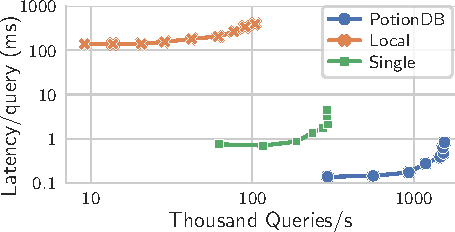
\includegraphics[width=0.6\linewidth]{singleQuery/all_queries_tc}
	\vspace*{-0.75em}
	\caption{Query-only performance of executing all queries.}
	\label{fig:global_local_single_tc}
	\vspace*{-0.9em}
\end{figure}%
\begin{figure}
	\centering
	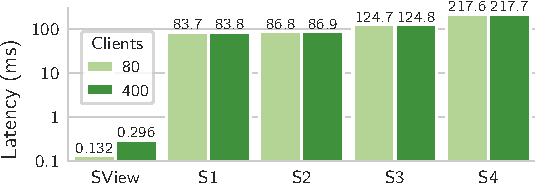
\includegraphics[width=0.72\linewidth]{singleQuery/single_TC_latencies}
	\vspace*{-0.6em}
	\caption{Average latencies of clients in Single PotionDB, depending on the server they are connected to.}
	\label{fig:single_tc_latencies}
	\vspace*{-0.9em}
\end{figure}%

Figure \ref{fig:global_local_single_tc} shows the results of running all selected TPC-H queries in PotionDB, Local PotionDB and Single PotionDB.
Each client executes one query per transaction.
Results are shown in queries/s versus average latency (RTT + execution time).

PotionDB's throughput reaches up to 1.5M queries/s, with latency varying between 0.15ms and 0.6ms, depending on the number of clients.
PotionDB's query performance is unaffected by the latency added between servers, as all server's views have the necessary information to reply to all queries.
%PotionDB's query performance is unaffected by latency - given all servers replicate every view, and every view is complete, PotionDB is able to reply to all queries with only a local read.
%PotionDB's performance can scale further if multiple queries are executed per transaction, as discussed in Section \ref{subsec:query_batching}.

Conversely, Local PotionDB is highly affected by latency.
On average, each client request takes 140ms to complete, as global queries (2/3rd of the queries) require data from all regions.
Global queries must to be forwarded and executed in all servers.
%This high latency is due to global queries (2/3rd of the queries) requiring information from all regions% - thus said queries need to be forwarded and executed in all servers.
%, which need to be forwarded and executed in all servers.
The remaining queries are local and are locally executed with low latency.
%The other 1/3rd are local queries which are executed locally with low latency.
%Each global query takes around 210ms, as all servers have one other server at a distance of at least 200ms.
%The other 1/3rd are local queries which are quickly executed with low latency, hence the average latency of 140ms.
%As will be seen in Section \ref{subsec:???}, global queries take around 210ms to execute in Local PotionDB, with local queries taking less than 1ms - hence the average latency of 140ms.
Local PotionDB's throughput is very low comparatively to PotionDB - executing each global query in all servers incurs extra server load and more network data transfers.
%Local PotionDB's throughput is very low comparatively to PotionDB - given global queries are processed everywhere, the servers incur an extra load and more data is transferred in the network.
Moreover, global queries' high latency caps each client's throughput to about 7 queries/s - thus several thousands of clients are required to saturate Local PotionDB.
At this point PotionDB spends most of the time managing thousands of connections and constantly swapping processor cores between threads, instead of on query execution.
%Furthermore, Local PotionDB's throughput is very low compared to PotionDB's, which can be explained with the following.
%First, each global query needs to be executed in all servers, adding extra load on each server and requiring more data to be transferred in the network.
%Second, due to the added latency, each client can only execute close to 5 global queries/s, thus thousands of clients are required to saturate PotionDB.
%At this point, PotionDB spends the majority of the time managing thousands of connections and constantly swapping processor cores between threads, instead of on query execution.
%Discuss SinglePotionDB

Finally, Single PotionDB's max throughput is roughly 1/5th of PotionDB's.
This is expected as all queries are served by views, which are all in one server (view server) that gets all the query load.
%This is expected as queries are entirely served by views which are all in the same server (view server), thus said server gets all the query load.
Given that 80\% of the clients are not connected to the view server, the average latency may seem unexpectedly low.
%This is expected as queries are entirely served by views, which are all in only 1 server out of the 5 servers - thus said server gets all the load, instead of it being evenly distributed.
%The latency may, at a first glance, seem unexpectedly low, given that 80\% of the clients suffer from latency due to their requests having to be re-forwarded to the server with views.
This happens as the view server's throughput is mostly consumed by clients directly connected to it, as other clients spend most of their time waiting for RTT.
This is common to all experiments of Single PotionDB with added latency.
%Figure \ref{fig:single_tc_latencies} shows the clients' latency grouped by server connection.
Figure \ref{fig:single_tc_latencies} gives a better overview of clients' latencies.
%Figure \ref{fig:single_tc_latencies} portrays more accurately the latencies experienced by clients. 
%Figure \ref{fig:single_tc_latencies} shows the average latencies of clients grouped by the server they are connected to.
%In practice the throughput is mostly consumed by the clients directly connected to the view server, as other clients spend most of their time waiting for RTT - consequently the average latency of all is low.
%This observation is applicable for all experiments of Single PotionDB with added latency.%, thus the graphic in Figure \ref{fig:single_tc_latencies} can be used as a reference for those experiments.
%Thus, Figure \ref{fig:single_tc_latencies} provides a more accurate representation of the latencies experienced by clients in Single PotionDB.
%This observation is appliable for all experiments of Single PotionDB with latency added between servers, thus we omit the equivalent to Figure \ref{fig:single_tc_latencies} in other experiments to avoid unnecessary repetition.

To conclude, having global, complete views replicated in every server allows all clients to achieve low latency and high throughput in PotionDB, while Local and Single PotionDB suffer from comparatively high latency and low throughput.

%In conclusion, having global, complete views replicated in every server allows all clients to achieve low latency and high throughput in PotionDB, while Local and Single PotionDB suffer from high latency and low throughput for, respectively, all global queries of all clients or in both local and global queries of clients faraway from the server with views. 

%\begin{itemize}
%	\item Graph with latency of all queries
%	\item Graph with latency of Q3; Q5
%	\item Two graphs with updates, side by side: one for PotionDB, one for Local PotionDB. Consider including single PotionDB albeit likely not needed (it is obvious this will not scale well as all transactions need to communicate with the view server).
%	\item (Keep explanations short on the ones above, as there is not much to comment - local has terrible latency (except for Q5), single is 1/5th of PotionDB with highly variable latency due to some clients being close and others faraway.)
%	\item Explain that latency benefits our solution (our solution is even more advantageous with latency than without latency when compared to Local and Single versions)
%	\item Graph without latency of all queries
%	\item Graph without latency of Q3; Q5
%	\item Graph with updates without latency (likely two graphs again)
%	\item (The three above is when we can give explanations on why local and single are always worse, even in their ideal scenarios.)
%	\item Before I used to have query and update latency graphs - are they still needed? These graphs show two things: (1), updates have higher latency than queries, mainly due to many updates needed to update an order, while to do a full "query trransaction", only 7 reads are needed to implement all 6 queries; (2) update latency spikes easily when the server saturates, due to many commits trying to get locks which enter in conflict.
%	\item query-only graph with different sizes for the K of TopK. Shows how much the size of the "limit" affects performance.
%	\item (I think we can cut the two old graphs that showed the performance with updates and different topK sizes)
%	\item bar graph that shows the "best" throughput for different sizes of K for both TopK and TopSum, and for different update rates. (maybe modify the graph to include the latency too that gives said throughput?)
%	\item bar graph that compares counter, average and topk for different numbers of replicas and update rates
%\end{itemize}

%\begin{figure}[h]
%	\centering
%	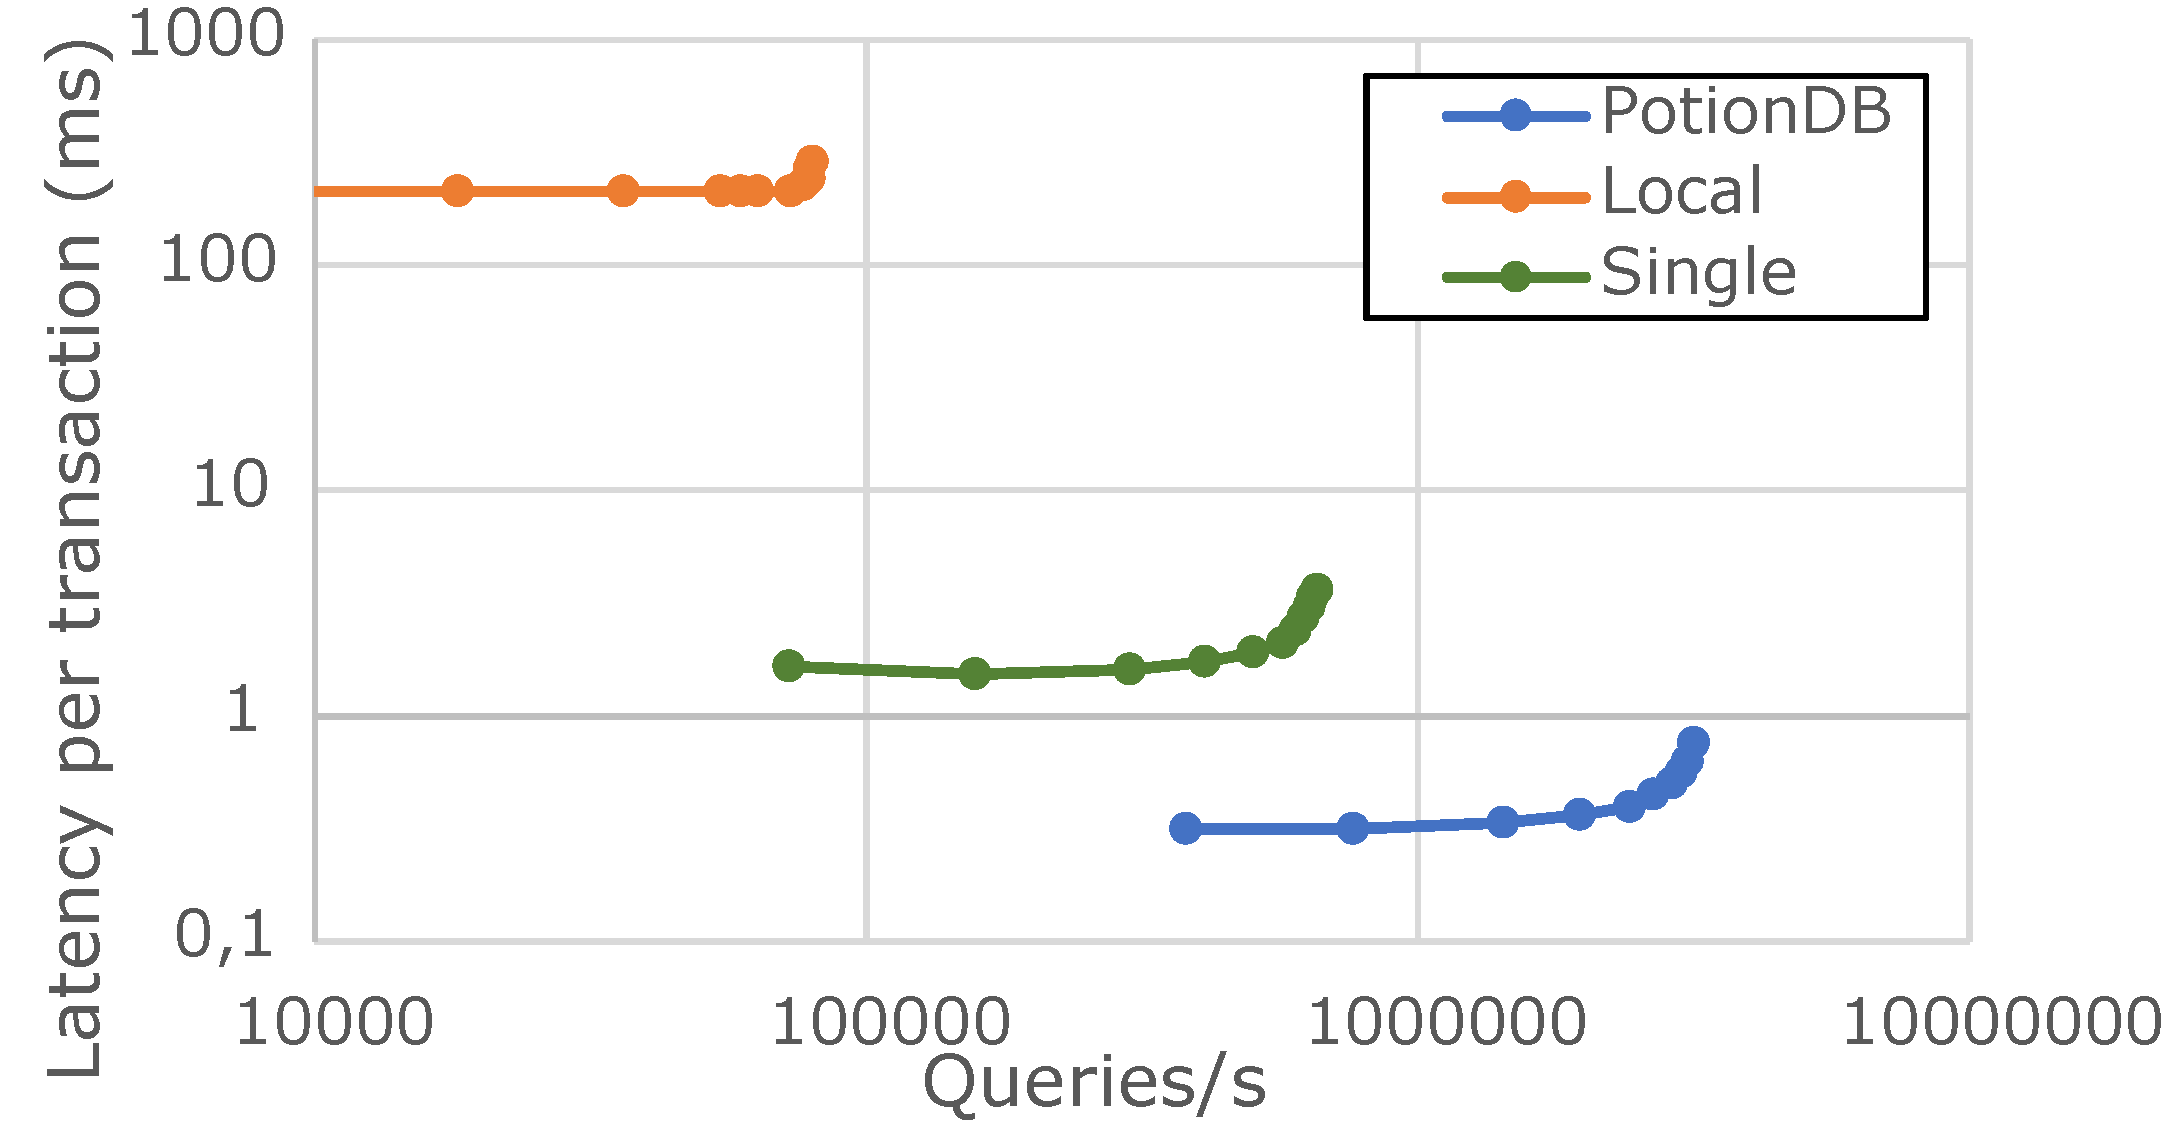
\includegraphics[width=1\linewidth]{clientScale_tc_cut}
%	\caption{[OLD]PotionDB's performance executing all queries. (1txn = all queries (6 queries, 7 reads total)).}
%	\label{fig:(new)global_local_single_tc}
%\end{figure}
%
%Note: Figure \ref{fig:(new)global_local_single_tc} will, later on, show the variation of latency for at least the single version.
%\begin{itemize}
%	\item Short introduction (we try to evaluate the benefits of global views replicated everywhere; compare with other two versions; access scalability in throughput and latency)
%	\item Explain how PotionDB is unaffected by latency;
%	\item Explain why Local PotionDB is so heavily affected by latency; also why low throughput (intuition: each global query ends up having to be re-forwarded to every server). Mention how 2/3rd of the queries require global data.
%	\item Explain why Single PotionDB is mildly affected by the latency (throughput dominated by clients close to the server. Faraway clients (i.e., most of the clients) experience low throughput and high latency).
%\end{itemize}

%TODO: Effects of query locality or data locality?
\subsubsection{Effects of query locality}
\label{subsec:data_locality}

\begin{figure}
	\centering
	\begin{subfigure}{.49\linewidth}
		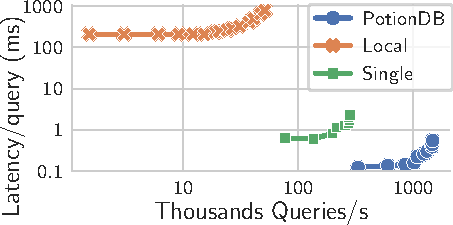
\includegraphics[width=1\linewidth]{singleQuery/q3_latency}
		\caption{Q3-only (global query).}
		\label{fig:q3_tc}
	\end{subfigure}%
	\hspace*{0.2em}
	\begin{subfigure}{.49\linewidth}
		%\raggedright
		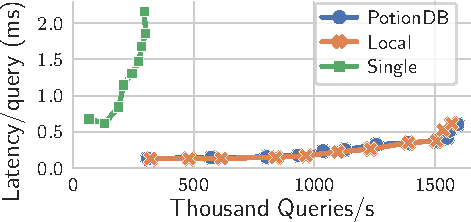
\includegraphics[width=1\linewidth]{singleQuery/q5_latency}
		\caption{Q5-only (local query).}
		\label{fig:q5_tc}
	\end{subfigure}%
	\vspace*{-0.55em}
	\caption{Query performance when executing only Q3 or Q5.}
	\label{fig:q3_q5_tc}
	\vspace*{-1.1em}
\end{figure}

Figures \ref{fig:q3_tc} and \ref{fig:q5_tc} showcase the results of our experiments with clients running only, respectively, Query 3 (Q3, a global query) and Query 5 (Q5, a local query) in PotionDB, in Local and in Single PotionDB.

The aforementioned figures showcase how view locality affects Local PotionDB's performance.
Given Q5 only requires data of a region, Local PotionDB performs similarly to PotionDB, as the server has the required view data to answer the query directly.
For local queries, clients only query about their own region.
%Note that on queries of a region, clients only query regarding their own region - and each client is connected to the server of his/her region.
This is the equivalent of, e.g., in an e-commerce, querying the list of most popular products in the customer's country.
This is the ideal scenario for Local PotionDB, yet its performance is similar to PotionDB's - both achieve a max throughput of $\sim$1.6M ops/s and latencies starting at 0.15ms.

However, on Q3 (global query) data from all regions is required, thus on Local PotionDB high latency is observed and throughput is very low.
A single query takes on average 210ms to complete as for every server, the furthest away server has a latency of 203$\sim$217ms.
Throughput reaches only a mere 17k ops/s before latency increases even further due to the sheer amount of client connections.
Finally, regarding Single PotionDB, as expected for both queries the throughput is about 1/5th of PotionDB, as views are complete.

In short, PotionDB is efficient for both global and local queries, while Local PotionDB is heavily hindered by latency for any query that is not fully local.

%II have to do these two graphs (I have the necessary data however).
%Here's what those graphs will show.
%
%Graph one: Q3 (global query). PotionDB will scale fine, up to 4.5m ops/s, unnafected by latency (around 0.8ms at 4.5m ops/s). Local PotionDB will be a disaster, with around 210ms latency and up to 70k ops/s. Single PotionDB will get up to around 900k ops/s (1/5th of PotionDB), with around 3-4ms of latency (some effect from added latency).
%
%Graph two: Q5 (local query). PotionDB and Local PotionDB will scale similarly: respectively, 4.1m ops/s and 3.9m ops/s. Both are unaffected by added latency, Local PotionDB even has slightly lower latency. Single PotionDB will have 1/5th of their performance and around 3-4ms latency (i.e., some effect from added latency).
%
%\begin{itemize}
%	\item executing only global queries (Q3) further exacerbates how poorly Local PotionDB performs, due to having to contact all servers for each query. (similar conclusions to the previous section)
%	\item when executing local-only queries (Q5), local PotionDB performs similarly to PotionDB - no redirection of requests is needed (clients only ask for data of their region), thus local PotionDB can efficiently reply to queries with only its local data views. Our solution "does not lose" to the local view solution.
%\end{itemize}

\subsubsection{PotionDB scaling with updates}

%\begin{figure*}
%	\begin{subfigure}{0.31\linewidth}
%		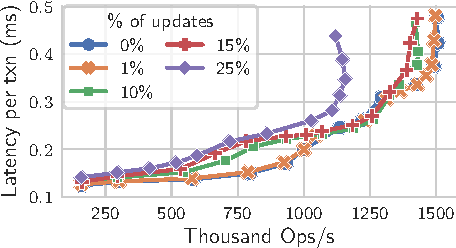
\includegraphics[width=1\linewidth]{singleQuery/upd_rate_global}
%		\caption{PotionDB.}
%		\label{fig:update_rates_global}
%	\end{subfigure}%
%	\hspace*{0.5em}
%	\begin{subfigure}{.31\linewidth}
%		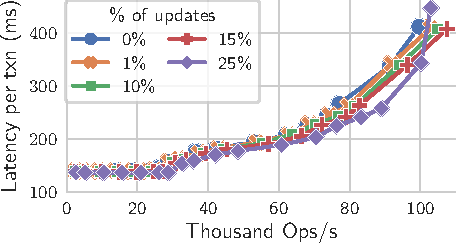
\includegraphics[width=1\linewidth]{singleQuery/upd_rate_local_tc}
%		\caption{Local PotionDB.}
%		\label{fig:update_rates_local_tc}
%	\end{subfigure}%
%	\hspace*{0.5em}
%	\begin{subfigure}{.31\linewidth}
%		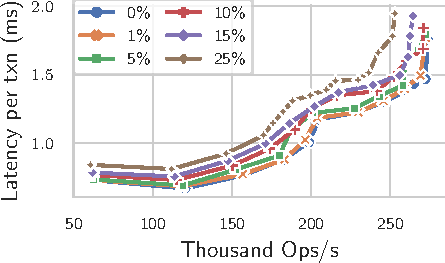
\includegraphics[width=1\linewidth]{singleQuery/upd_rate_single_tc}
%		\caption{Single PotionDB.}
%		\label{fig:update_rates_single_tc}
%	\end{subfigure}%
%	\vspace*{-0.75em}
%	\caption{From left to right, total throughput of PotionDB, Local PotionDB and Single PotionDB with a varying update rate.}
%	\label{fig:upds_tc}
%	\vspace*{-0.6em}
%\end{figure*}
\begin{figure}
	\centering
	\begin{subfigure}{.47\linewidth}
		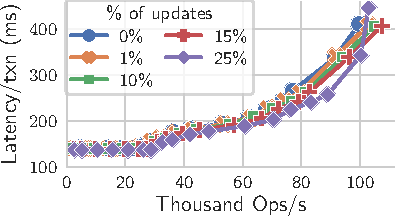
\includegraphics[width=1\linewidth]{singleQuery/upd_rate_local_tc_short}
		\caption{Local PotionDB}
		\label{fig:update_rates_local_tc}
	\end{subfigure}%
	\hspace*{0.2em}
	\begin{subfigure}{.52\linewidth}
		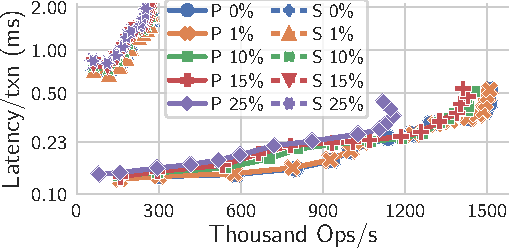
\includegraphics[width=1\linewidth]{singleQuery/upd_rate_tc_global_vs_single}
		\caption{PotionDB and \textit{Single} PotionDB}
		\label{fig:update_rates_global_single_tc}
	\end{subfigure}%
	\vspace*{-0.65em}
	\caption{Performance with multiple update rates.}
	\label{fig:upds_tc}
	\vspace*{-1.2em}
\end{figure}


We now evaluate the impact of executing updates alongside queries on PotionDB's throughput for multiple update/read ratios.
Clients pick randomly
%In this scenario, when a client wants to execute an operation, it picks randomly
whenever to execute a single query or an update transaction.
An update transaction consists in the creation of a new order, of its ordered items and all associated view updates.
%An update transaction consists in the creation of a new order, which also includes the necessary updates to create the items that were ordered and associated view updates.
%View updates are not counted for throughput.
The latter however is not counted towards throughput.
A 25\%/75\% ratio means that 25\% of all executed operations (including view updates) are updates.%, not that 25\% of the transactions are write-transactions.

%\begin{figure}
%	\centering
%	\begin{subfigure}{.49\linewidth}
%		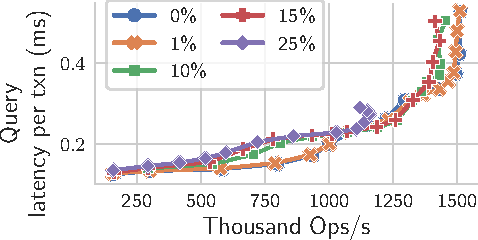
\includegraphics[width=1\linewidth]{singleQuery/query_latency_global}
%		\caption{Query-latency.}
%		\label{fig:query_latency}
%	\end{subfigure}%
%	\hspace*{0.8em}
%	\begin{subfigure}{.49\linewidth}
%		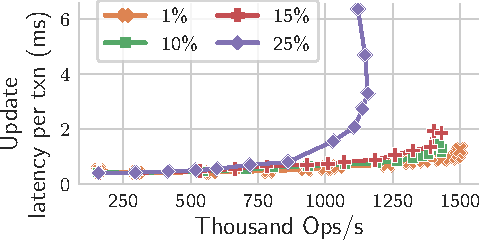
\includegraphics[width=1\linewidth]{singleQuery/upd_latency_global}
%		\caption{Update-latency.}
%		\label{fig:update_latency}
%	\end{subfigure}
%	\caption{Average latencies of queries and updates on PotionDB.}
%\end{figure}

%0: 1.511M ops/s, 0.01: 1.517M ops/s,  0.05: 1.46M, 0.1: 1.45M, 0.15: 1.43M, 0.25: 1.157M
Figure \ref{fig:upds_tc} shows the results of executing updates alongside queries with multiple update/read ratios.
%PotionDB has small throughput losses for modest update rates (between 0.1\% and 5.4\% for update rates up to 15\%), while for 25\% it has a significant drop of 23.4\%.
In PotionDB, for 1\% update rate, the impact is unnoticeable.
The throughput drop for modest update rates (10\% and 15\%) is reasonable (4\% and 5.4\%), while for 25\% it is quite more significant (23.4\%).
The lower max throughput and slightly higher latencies are due to the following.
Update transactions apply the commit protocol locally (Section \ref{subsec:commit}), which requires coordination of multiple shards (multiple updates per transaction), which leads to an higher latency than with queries.
%Moreover, if too many update transactions are issued concurrently, they will have to wait for each other, increasing the average latency.
Note however that queries' latency only raises lightly as in practice they seldom wait for updates.
%25\%: 0.273304; 0\%: 0.245562
For instance, at PotionDB's max throughput for 25\% updates, its query-only latency and the corresponding for 0\% are, respectively, 0.273ms and 0.246ms.

%To execute an update transaction, shards have to synchronize to apply the commit protocol (Section \ref{subsec:commit}) - thus, as the update rate gets higher, this synchronization happens more often, potentially making other queries/updates wait.
%This synchronization, as well as multiple updates being in the same transaction, is why update transactions have higher latency than queries, as seen on Figure \ref{fig:update_latency}.
%We note however that in practice queries seldom have to wait for updates unless the server is saturated, as can be seen in Figure \ref{fig:query_latency}.
%The main observable difference in query latency is the latency at the middle of the throughput raising earlier.
%We believe this may be due to network artifacts that lead to latency raising slightly when using over a certain amount of bandwidth - since update transactions have many updates, this threshold is reached with less clients. %TODO: This is... not really a good explanation. Sigh

Local PotionDB benefits from having multiple updates per transaction, as more operations are done per RTT.
Thus, Local PotionDB's max throughput raises slightly as the update ratio rises, as seen on Figure \ref{fig:update_rates_local_tc}.
%Updates do not hinder Local PotionDB considerably, as seen on Figure \ref{fig:update_rates_local_tc}.
%The latency experienced between servers means Local PotionDB benefits from grouping updates in a single transaction, as more operations can be done per RTT - hence the slight rise in throughput.
Plus, update transactions do not need to contact every server, as 50\% of the orders are local to a region, \footnote{This does not occur on the original TPC-H dataset, whose orders' items are random. This modification adds locality to orders, which is more realistic for an e-commerce scenario and helps Local PotionDB more than PotionDB.
	%Note that this helps Local PotionDB more than PotionDB.
} while most others refer few regions - hence the slightly lower average latency with higher update rates.
Note that if queries were grouped, throughput would raise further.
%Note that if queries were grouped, throughput would raise even more, as queries still dominate the workload
%Note that grouping of queries would increase throughput even more considerably.
%Note that if queries were grouped, the increase in throughput would be more considerable, as queries still dominate the workload.

%fig:update_rates_single_tc
Single PotionDB (Figure \ref{fig:update_rates_global_single_tc}) has throughput losses comparable to PotionDB's, except for 25\% updates where the percentage of loss is smaller than PotionDB's due to not having to replicate view updates.
%Single PotionDB (Figure \ref{fig:update_rates_single_tc}) has similar results to PotionDB, except for 25\% where the percentage of loss throughput is smaller compared to PotionDB, due to not having to replicate view updates.
However, even for 25\% updates, Single PotionDB's throughput is less than 1/4 of PotionDB's.
%For Single PotionDB (Figure \ref{fig:update_rates_single_tc}) the results are similar to PotionDB, except for 25\% update rate where Single PotionDB loses less percentage of throughput comparatively, due to not having to replicate view updates.
%Still, the max throughput of Single PotionDB even in this case is more than 3 times less than PotionDB's.
%Nevertheless, with more modest update rates the loss on throughput is comparable between both solutions - our solution is optimized for a read-heavy scenario like an e-commerce application, where users see many more products/listings than the ones they buy.
%We emphasize that our queries are complex queries, which would take several milliseconds or more to execute without views instead of sub-millisecond.

In summary, PotionDB still scales well with modest update rates as is common in, e.g., e-commerce applications.
%, with only a significant throughput loss in update-heavy scenarios, which are outside of PotionDB's usage scope.
PotionDB keeps views updated while answering complex global queries in sub-millisecond time.
%in less than 0.5ms.
%PotionDB is thus able to keep views up-to-date while still answering complex global queries in sub-millisecond time.
Moreover, updates in PotionDB are unaffected by latency between servers.
%Moreover, updates in PotionDB and Single PotionDB are unaffected by latency between servers.
%, as transactions are committed locally.
%TODO: I would like to re-add the phrase below if there is a little bit of space.
%The added latency only affects replication, so clients in other servers will take longer to notice the effects of updates executed in faraway servers. %Does this need some ending justification on how this is ok? %Also maybe remove this last two phrases?


%Two to three graphs: global with updates, local with updates, (optionally) single with updates. I have to modify the graphs to not count with updates for the views.
%
%Note: both graphs below still account for view updates on their throughput. 
%View updates account for around 2/3rd of the update count.
%
%%Graph global: higher update rates mean lower max throughput and a bit higher latency (e.g., 0\% updates starts at 0.3ms, 100\% starts at 0.5ms). The old graph of this one (still counting with view updates) is on Figure \ref{fig:(new)update_rates}.
%%Graph global: Check Figure \ref{fig:(new)update_rates}
%
%\begin{figure}[h]
%	\centering
%	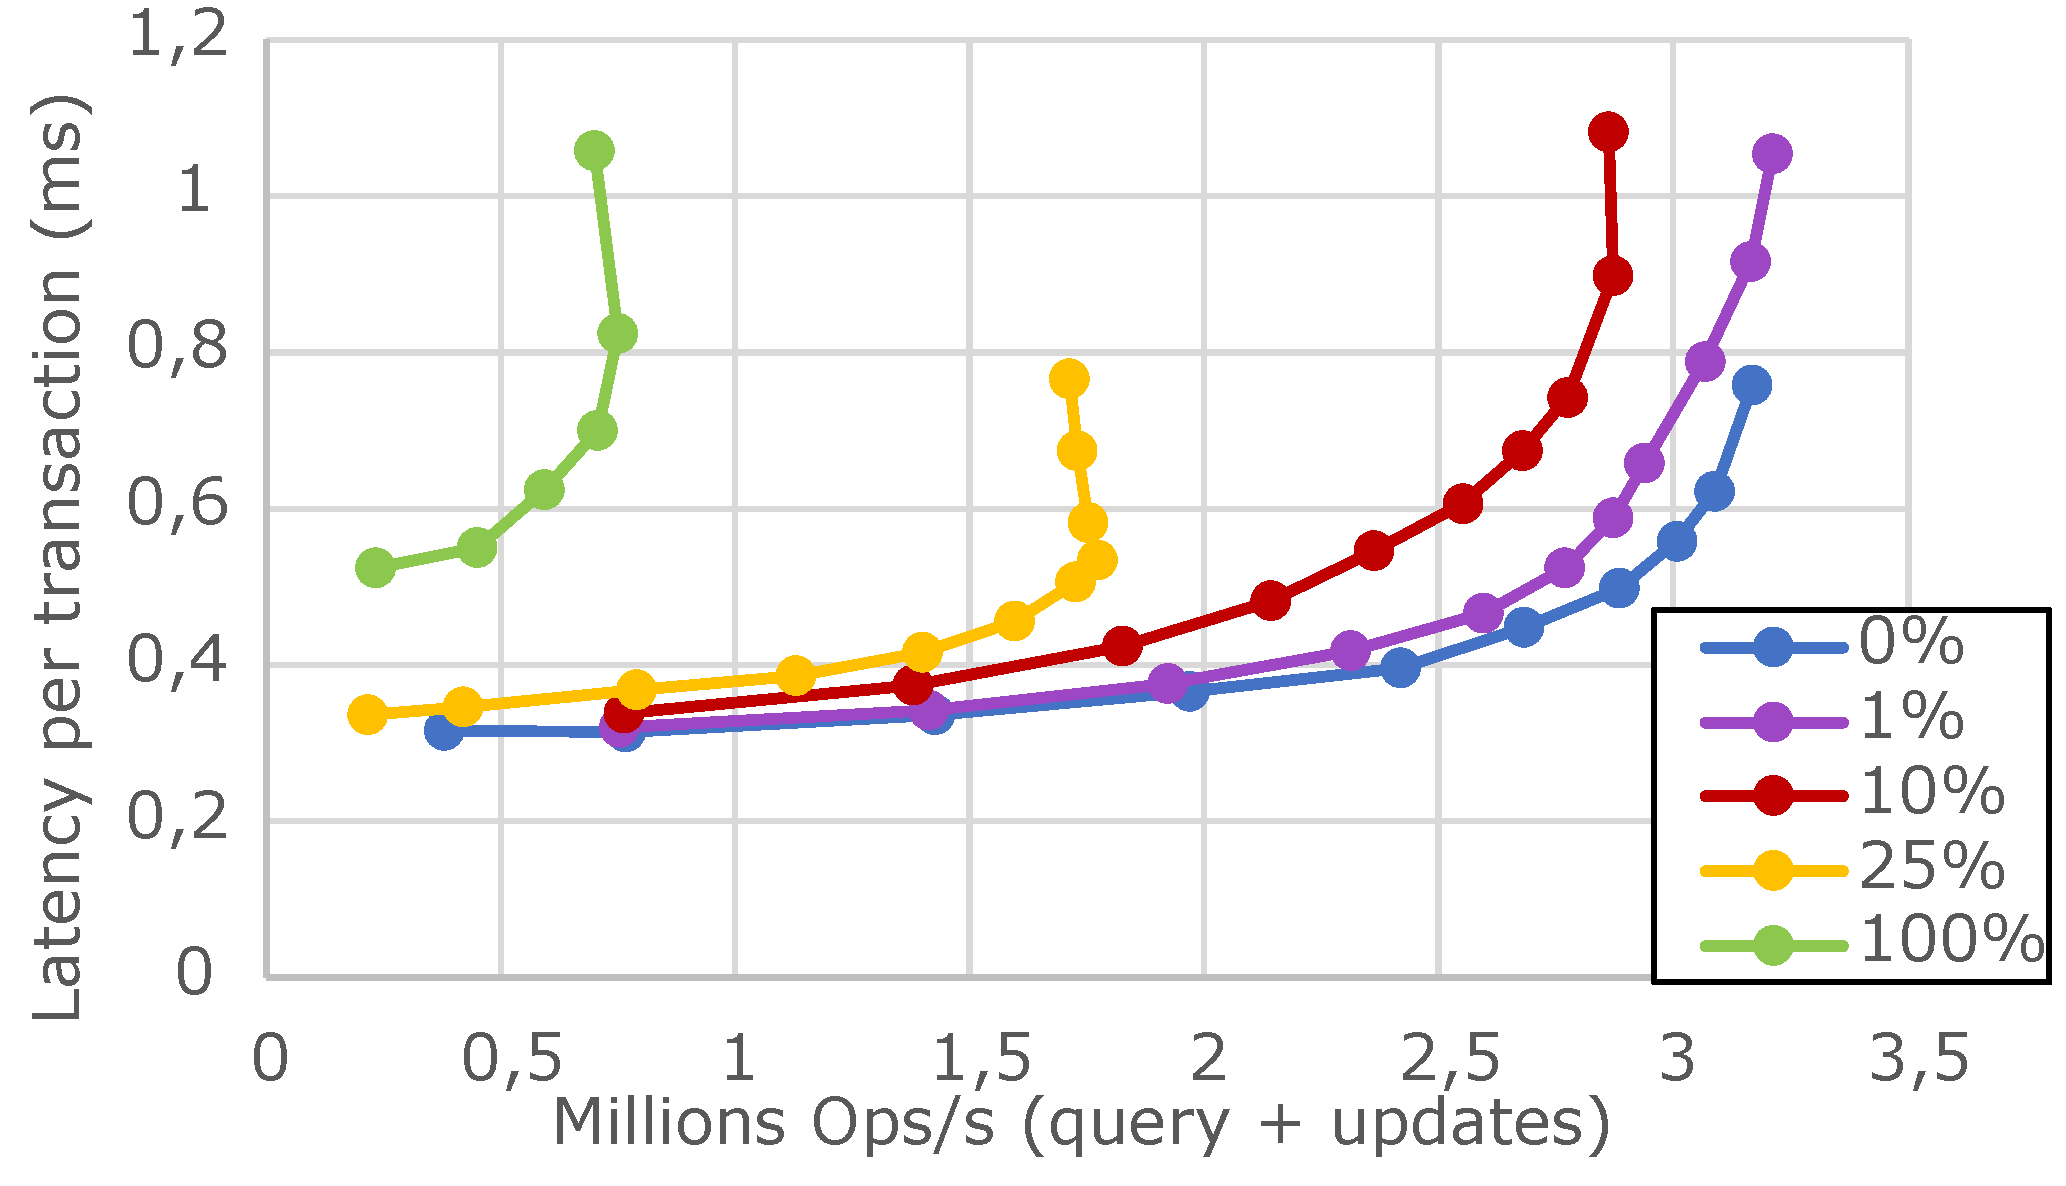
\includegraphics[width=.75\linewidth]{updRate_global_cut}
%	\caption{PotionDB's performance with varying update rate.}
%	\label{fig:(new)update_rates}
%\end{figure}
%
%\begin{figure}[h]
%	\centering
%	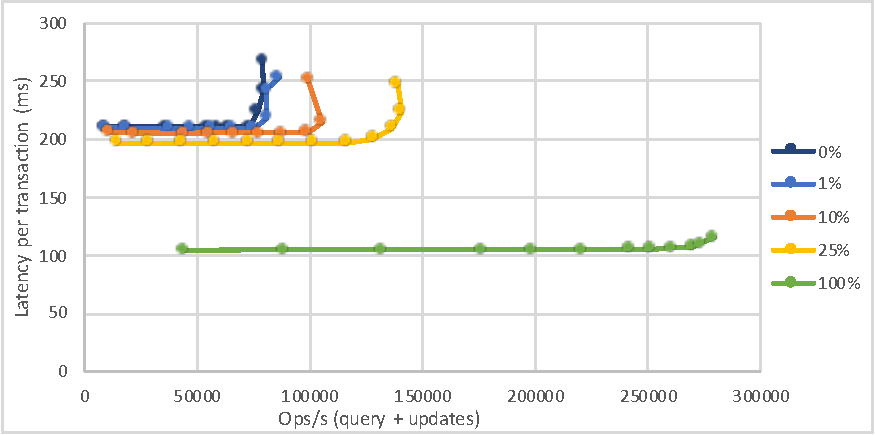
\includegraphics[width=.7\linewidth]{updRate_tc_cut}
%	\caption{Local PotionDB's performance with varying update rate}
%	\label{fig:(new)update_rates_tc}
%\end{figure}
%
%%Graph local: Low max throughput and high latency. Increasing the update ratio decreases latency slightly and increases max throughput con
%
%\begin{itemize}
%	\item Explain what is an update in TPC-H; explain how we do not count with view updates for the throughput;
%	\item Explain why PotionDB is unaffected by the added latency; explain why PotionDB's throughput decreases so heavily. Mention that a lot of the operations are not counted, as there are many view updates.
%	\item Explain why Local PotionDB is affected by the added latency. Explain why Local PotionDB's throughput increases with the higher update ratio and why latency decreases (reason: updates have lower latency than queries because only a subset of the servers need to be contacted, instead of all, so often the highest latency connection can be avoided. Furthermore, updates have more operations per transaction than queries, i.e., more operations per round trip.)
%\end{itemize}

\subsection{PotionDB performance on a single data center}

All experiments so far had latency imposed between servers to simulate a geo-distributed scenario.
This scenario benefits PotionDB compared to the other analysed solutions, as all queries and updates execute locally in the client's server.
%This scenario benefits PotionDB compared to the other analysed solutions, given both global and local queries, as well as any updates, execute fully in the replica the client is connected to.
Thus, we now evaluate if PotionDB is still ideal in a single data center scenario, i.e., without added latency. %between servers.

\begin{figure}
	\centering
	\begin{subfigure}{.49\linewidth}
		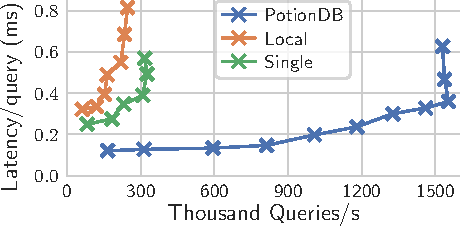
\includegraphics[width=1\linewidth]{singleQuery/all_queries_noTC}
		\caption{All queries}
		\label{fig:all_queries_noTC}
	\end{subfigure}%
	\hspace*{0.2em}
	\begin{subfigure}{.49\linewidth}
		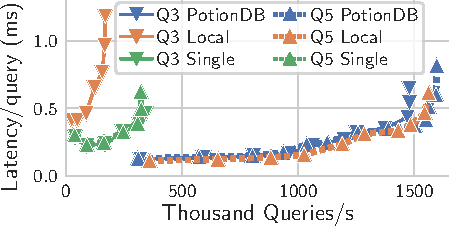
\includegraphics[width=1\linewidth]{singleQuery/q3_q5_noLatency}
		\caption{Single type of query}
		\label{fig:q3_q5_noTC}
	\end{subfigure}%
	\vspace*{-0.65em}
	\caption{Query performance with no added latency.}
	\label{fig:global_local_single_noTC}
	\vspace*{-1.2em}
\end{figure}

Figure \ref{fig:global_local_single_noTC} shows PotionDB, Local PotionDB and Single PotionDB's query performance without added latency.
Compared to previous experiments, PotionDB shows no difference.
Single 
PotionDB has slightly higher throughput and lower latency, as all clients are now effectively close to the view server, despite many queries being forwarded from other servers. %I feel this is not clear. But basically, no latency between servers implies that even with redirection of requests, the latency is low.
%PotionDB shows no difference compared to %the experiments featuring added latency.
%previous experiments.
%Single PotionDB features slightly higher throughput and considerably lower average latency compared to previous experiments, as all clients are now effectively close to the view server, even though many requests are forwarded from other servers.
%The latter is because with latency added, sudden spikes of load happen when the requests from faraway clients finally arrive, instead of the load being well distributed.
%Furthermore, forwarded requests are not as efficient due to extra serialization, deserialization and data transfer.
%I think I don't need to justify the higher throughput as it's a slight difference.

With Local PotionDB, when considering only local queries like Q5 in Figure \ref{fig:q3_q5_noTC}, performance is the same as previously observed as those queries are served locally.
However, when considering only global queries, Local PotionDB still performs poorly - e.g., with Q3, its max throughput is 180k queries/s, which is only 12\% of PotionDB's 1.5M queries/s.
Even when factoring in all global and local queries (Figure \ref{fig:all_queries_noTC}), Local PotionDB's throughput is less than 17\% of PotionDB's, as in the former global queries contact all servers.
%However, even without added latency, Local PotionDB's performance is quite lower than PotionDB's when including global queries, as seen in Figures \ref{fig:all_queries_noTC} and \ref{fig:q3_q5_noTC}.
%For instance, with only Q3, Local PotionDB's max throughput is only $\sim$12\% of PotionDB's - respectively, close to 180k and 1.5M queries/s.
%Even when factoring both global and local queries, Local PotionDB's throughput is less than 17\% of PotionDB's, as in the former global queries have to be executed in all servers. %not to mention the higher latency
%This is due to global queries needing to be processed in every server in Local PotionDB, thus leading to a higher server load, more data transferred and higher latency.
%This is due to, in Local PotionDB, global queries needing to be processed in every server, which imposes an higher load in the servers and requiring more data to be transferred, which also increases the processing time spent on serializing/deserializing data.

\begin{figure}
	\centering
	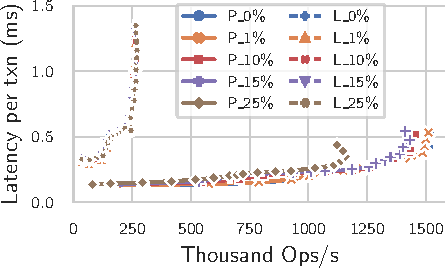
\includegraphics[width=0.62\linewidth]{singleQuery/upd_rate_noTC_global_vs_local}
	%\vspace*{-0.65em}
	\caption{PotionDB and Local PotionDB's performance with multiple update rates, without added latency.}
	\label{fig:update_rates_global_vs_local_noTC}
	%\vspace*{-0em}
\end{figure}

%TODO: Would be really nice if I could trim this one further
In scenarios with updates, similar conclusions can be taken - Figure \ref{fig:update_rates_global_vs_local_noTC} showcases PotionDB's and Local PotionDB's throughputs for multiple update rates.
PotionDB's throughput is the same as previously in Figure \ref{fig:update_rates_global_single_tc}.
%PotionDB is the same as previously observed in Figure \ref{fig:update_rates_global_single_tc}. %, given latency between servers does not affect PotionDB's performance.
Local PotionDB's throughput only reaches $\sim$250k ops/s for all update rates.
%For Local PotionDB, the throughput is lower than PotionDB's in all cases, staying at around 250k ops/s for all update rates.
The stability of Local PotionDB's throughput across different update rates is threefold:
%Local PotionDB's stable throughput across different update rates is threefold:
\begin{enumerate*}[label=(\roman*)]
	\item multiple updates per transaction;%, unlike queries which are one per transaction;
	\item orders' locality, thus many update transactions are local;
	%\item orders' locality implies half of update transactions are fully local and most others involve only a subset of servers;
	\item view updates are not replicated as views are local, which slightly reduces server load. %"do not need to be replicated" instead of "are not replicated"
	%\item view updates do not need to be replicated unlike in PotionDB as views are local, thus slightly reducing server load.
	%\item orders' locality implies that half of update transactions can be executed fully locally, with most others only requiring a subset of servers, unlike global queries which require all servers;
	%\item since views are local, view updates do not need to be replicated and applied in other servers, thus slightly reducing server load.
\end{enumerate*} %This still has some overlap with the previous section
Update scenarios favour Local PotionDB, yet its performance is far from PotionDB's.
%Even though scenarios with updates are favourable for Local PotionDB, it still does not match PotionDB's performance even with an high update ratio.
Finally, Single PotionDB's thoughput is similar to what was observed in Figure \ref{fig:update_rates_global_single_tc} (and thus lower than PotionDB's), but with lower latencies ranging from 0.24ms to 0.6ms.
%Finally, Single PotionDB achieves a throughput similar to what was observed previously in Figure \ref{fig:update_rates_single_tc}, but with smaller latencies, ranging from 0.2ms to 0.6ms.
%Its throughput is, thus, still always lower than PotionDB's.

%\begin{figure}
%	\centering
%	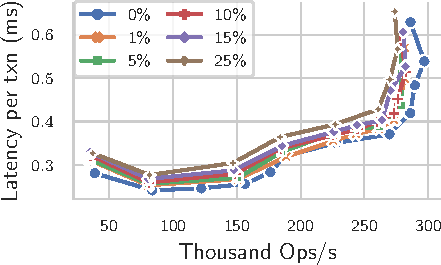
\includegraphics[width=1\linewidth]{singleQuery/upd_rate_single_noTC}
%	\caption{Single PotionDB's performance in multiple read:update ratios, with no latency added between servers.}
%	\label{fig:update_rates_single_noTC}
%\end{figure}

%Figure \ref{fig:update_rates_single_noTC} shows Single PotionDB's behaviour with updates.
%The throughput decreases as the update ratio increases, but with a smaller decrease than in PotionDB, similarly to what was observed in the scenario with latency.

%\begin{figure}
%	\centering
%	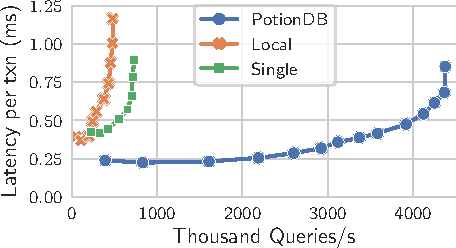
\includegraphics[width=0.62\linewidth]{singleQuery/all_queries_batch5_noTC}
%	\vspace*{-0.7em}
%	\caption{Query-only performance with all types of queries and with 5 queries per transaction.}
%	\label{fig:global_local_single_batch_notc}
%	\vspace*{-0.8em}
%\end{figure}

%To conclude, PotionDB is able to outperform Single and Local PotionDB in every scenario
To conclude, PotionDB's global views provide query throughputs and latencies unmatched by both Local and Single PotionDB in every tested scenario.
%To conclude, while PotionDB is favoured by a geo-distributed scenario relatively to Local and Single PotionDBs, even in a single data center scenario PotionDB's replicated global views still provide query throughputs and latencies unmatched by both Local and Single PotionDB.
As a side note, PotionDB scales further if clients issue multiple queries per transaction - e.g., with 5 queries/transaction, PotionDB's max throughput (resp. transaction latency) goes from 1.5M ops/s (0.37 ms) to 4.83M ops/s (0.68 ms), an increase of 222\% (83.8\%).
%Local and Single PotionDB's throughput also increase but with a smaller factor. %TODO: Consider removing this last phrase.
%As a side note, PotionDB's throughput scales even further if clients request multiple queries per transaction, as shown in Figure \ref{fig:global_local_single_batch_notc}.

%\subsection{Query batching}
%\label{subsec:query_batching}
%
%\begin{figure}
%	\centering
%	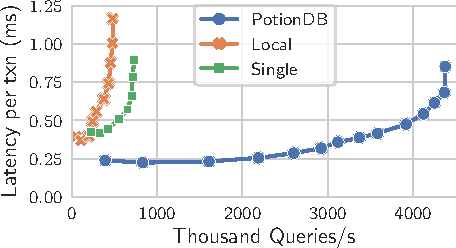
\includegraphics[width=0.7\linewidth]{singleQuery/all_queries_batch5_noTC}
%	\caption{Query-only performance of PotionDB, Local PotionDB and Single PotionDB with all types of queries, 5 queries per transaction}
%	\label{fig:global_local_single_batch_notc}
%\end{figure}
%
%In all previous experiments, each client executes only one query per transaction.
%Said situation does not allow for full usage of PotionDB's throughput.
%As an example, Figure \ref{fig:global_local_single_batch_notc} shows the query throughput of PotionDB, Local PotionDB and Single PotionDB when clients execute 5 queries per transaction.
%The higher throughput is noticeable - for instance, PotionDB's max throughput is almost 3 times higher compared to only 1 query per transaction. %Could say here or somewhere else this is because one of the queries is a Top100, which does not scale very well with batching
 
%Note: The idea here is to repeat all the tests before without latency and notice how our solution is still better than local and single PotionDB.
%
%\begin{itemize}
%	\item Explain how latency favours our solution over local and single PotionDB (i.e., our solution is unnafected by latency)
%	\item Explain that is why from here on we will test on a single DC, which benefits local and single
%\end{itemize}
%
%%Need to add graphs, these ones I believe I have on the paper already
%
%\begin{figure}[h]
%	\centering
%	\begin{subfigure}{.5\linewidth}
%		\centering
%		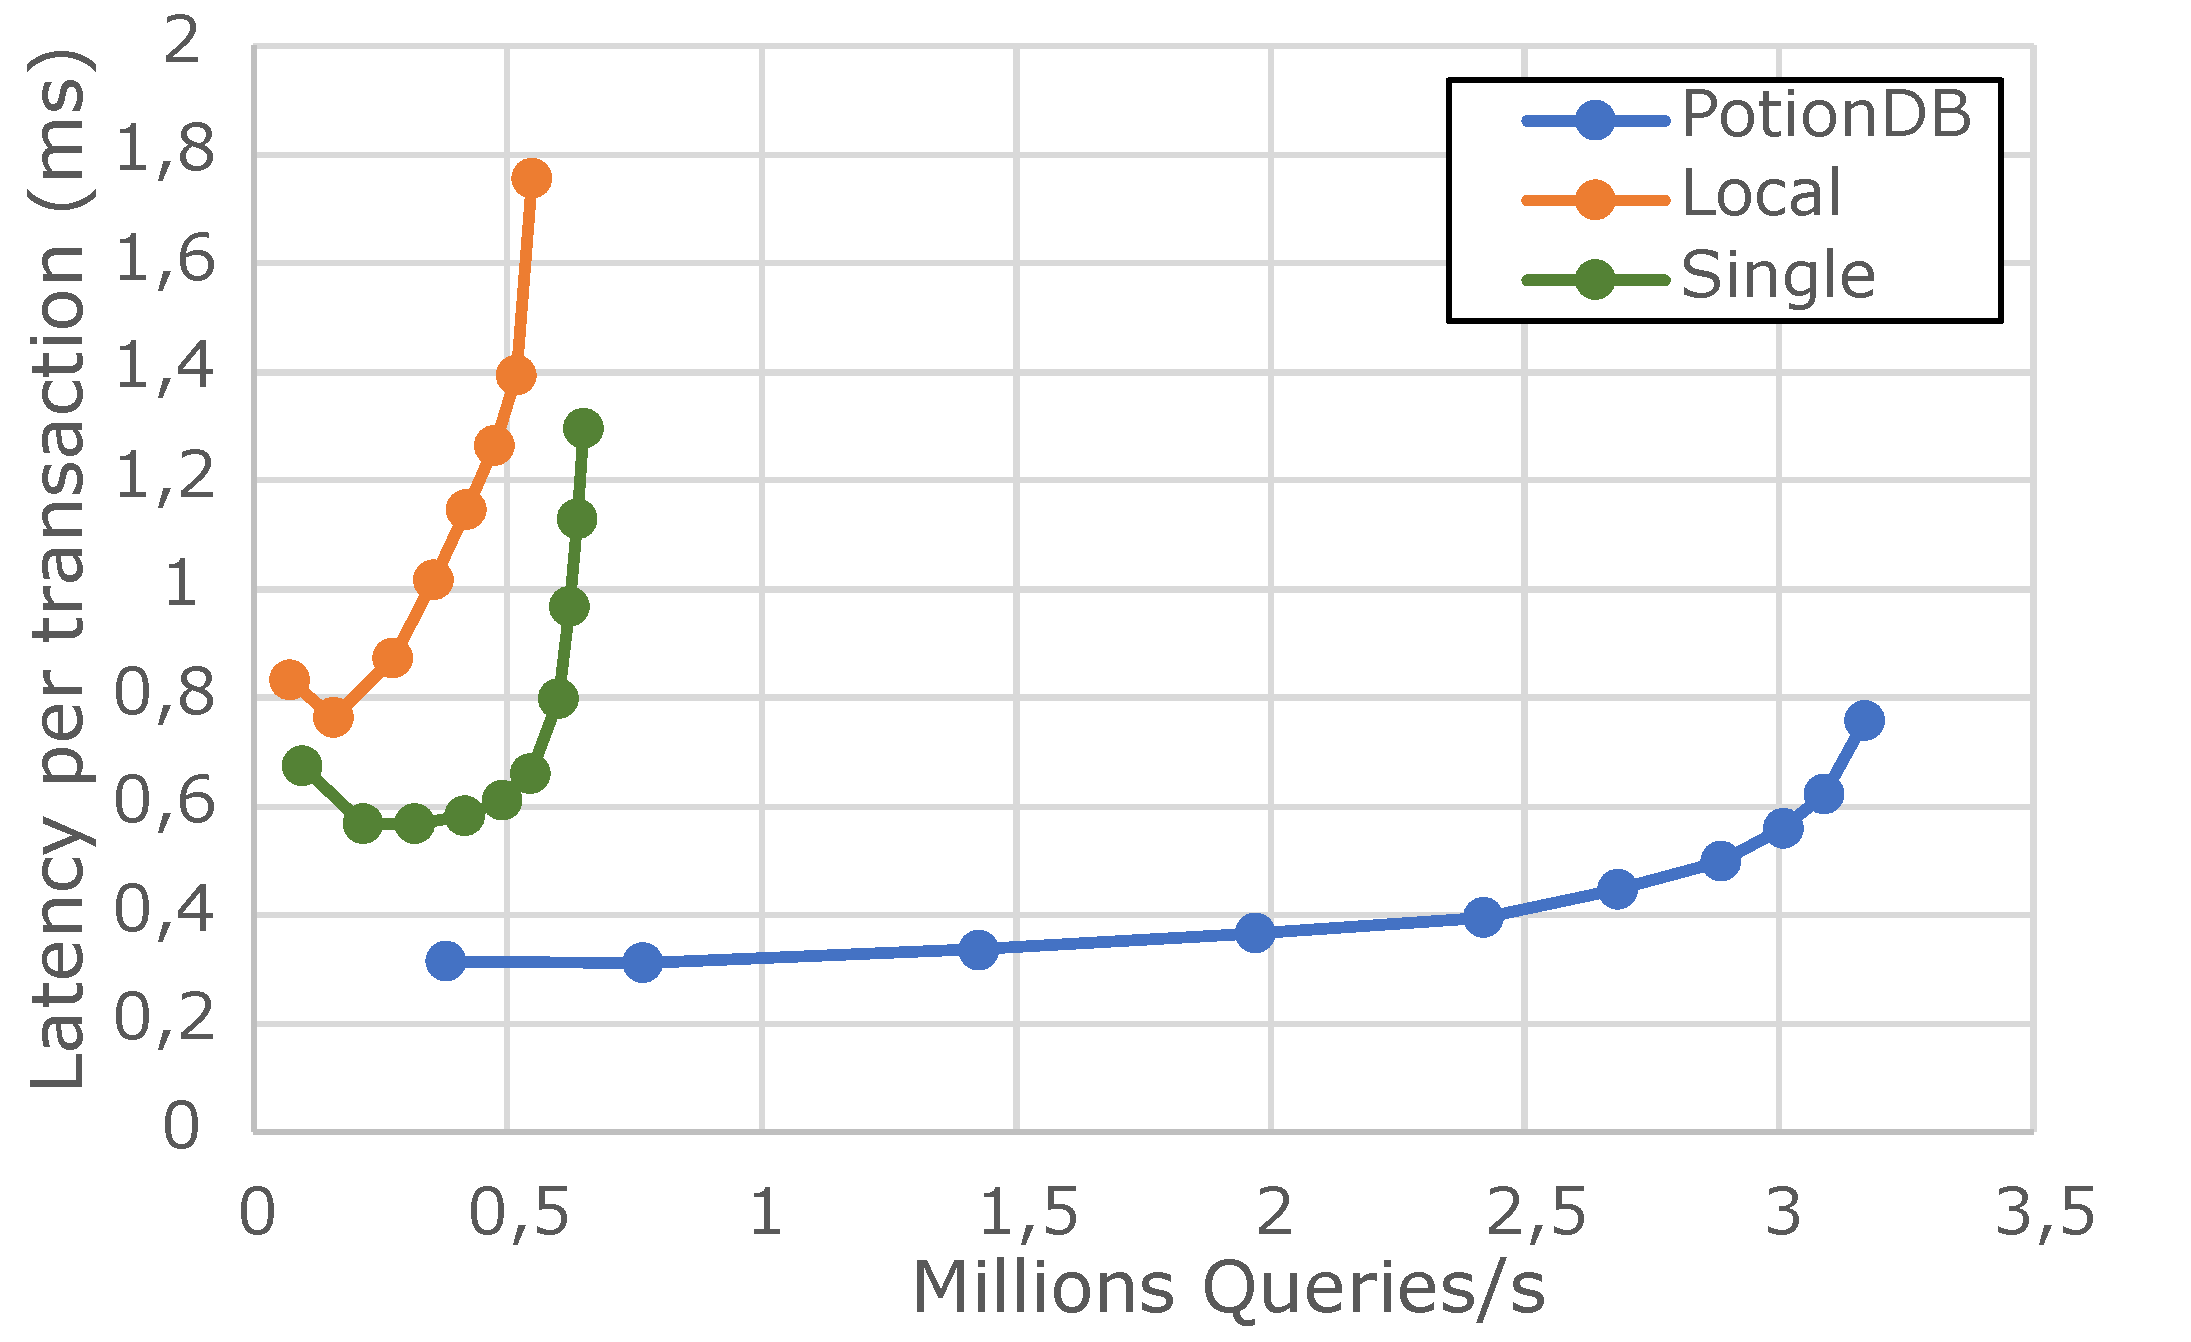
\includegraphics[width=.9\linewidth]{clientScale_cut}
%		\caption{All queries}
%		\label{fig:(new)global_local_single}
%	\end{subfigure}%
%	\begin{subfigure}{.5\linewidth}
%		\centering
%		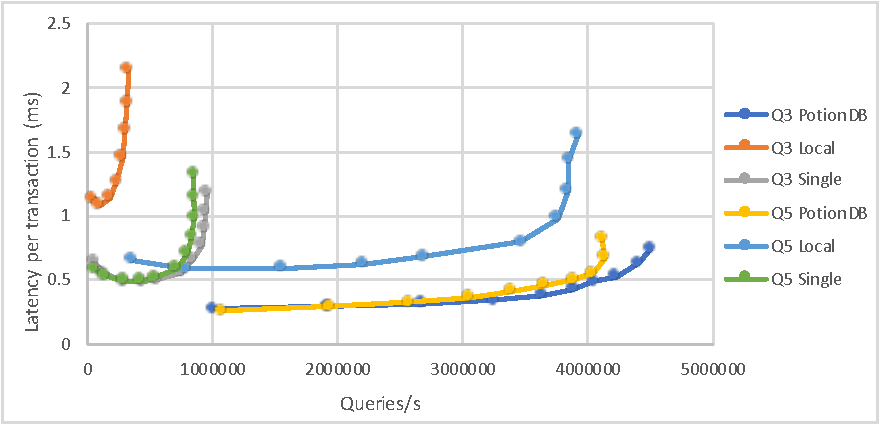
\includegraphics[width=.9\linewidth]{Q3vsQ5_cut}
%		\caption{Single query type}
%		\label{fig:(new)q3q5}
%	\end{subfigure}
%	\caption{Query-only performance of PotionDB and its local and single view versions, without added latency. On the left all queries are executed, while on the right only Q3 or Q5 are.}
%	\label{fig:(new)query_only}
%\end{figure}
%
%\begin{itemize}
%	\item Can confirm that PotionDB's performance is unaffected by added latency - same performance as before.
%	\item Local and single PotionDB still perform much worse than PotionDB when executing all queries.
%	\item Local PotionDB performance for all queries is around 1/6th of PotionDB. This is due to 2/3rd of the queries requiring data from all servers, which means needing to redirect requests and adding extra load on all servers, as well as having to wait for RTT. Furthermore, it implies all transactions need to wait for the slowest server. (Note: these redirected requests do not count for throughput - i.e., if a query only needed a single read in normal PotionDB, we only count as one read even if all servers need to execute said read)
%	\item Local PotionDB works well for Q5, as this query is served totally with data of a region (i.e., local data). For queries of a region, the clients always pick the region of the server they are connected to. Thus, no redirects occurs and its performance is comparable to PotionDB.
%	\item Local PotionDB does not perform well with Q3, a query requiring global data. The performance is only 1/13th of PotionDB's. This is due to the redirected requests, exercing extra pressure on all servers, the extra round-trip and bigger data transfers. (Note: this query is a top 10, thus the data transferred is non-negligible.)
%	\item Single PotionDB's max throughput is about 1/5th of PotionDB's performance for all scenarios considered, as one server gets the full load.
%\end{itemize}
%
%\begin{figure}[h]
%	\centering
%	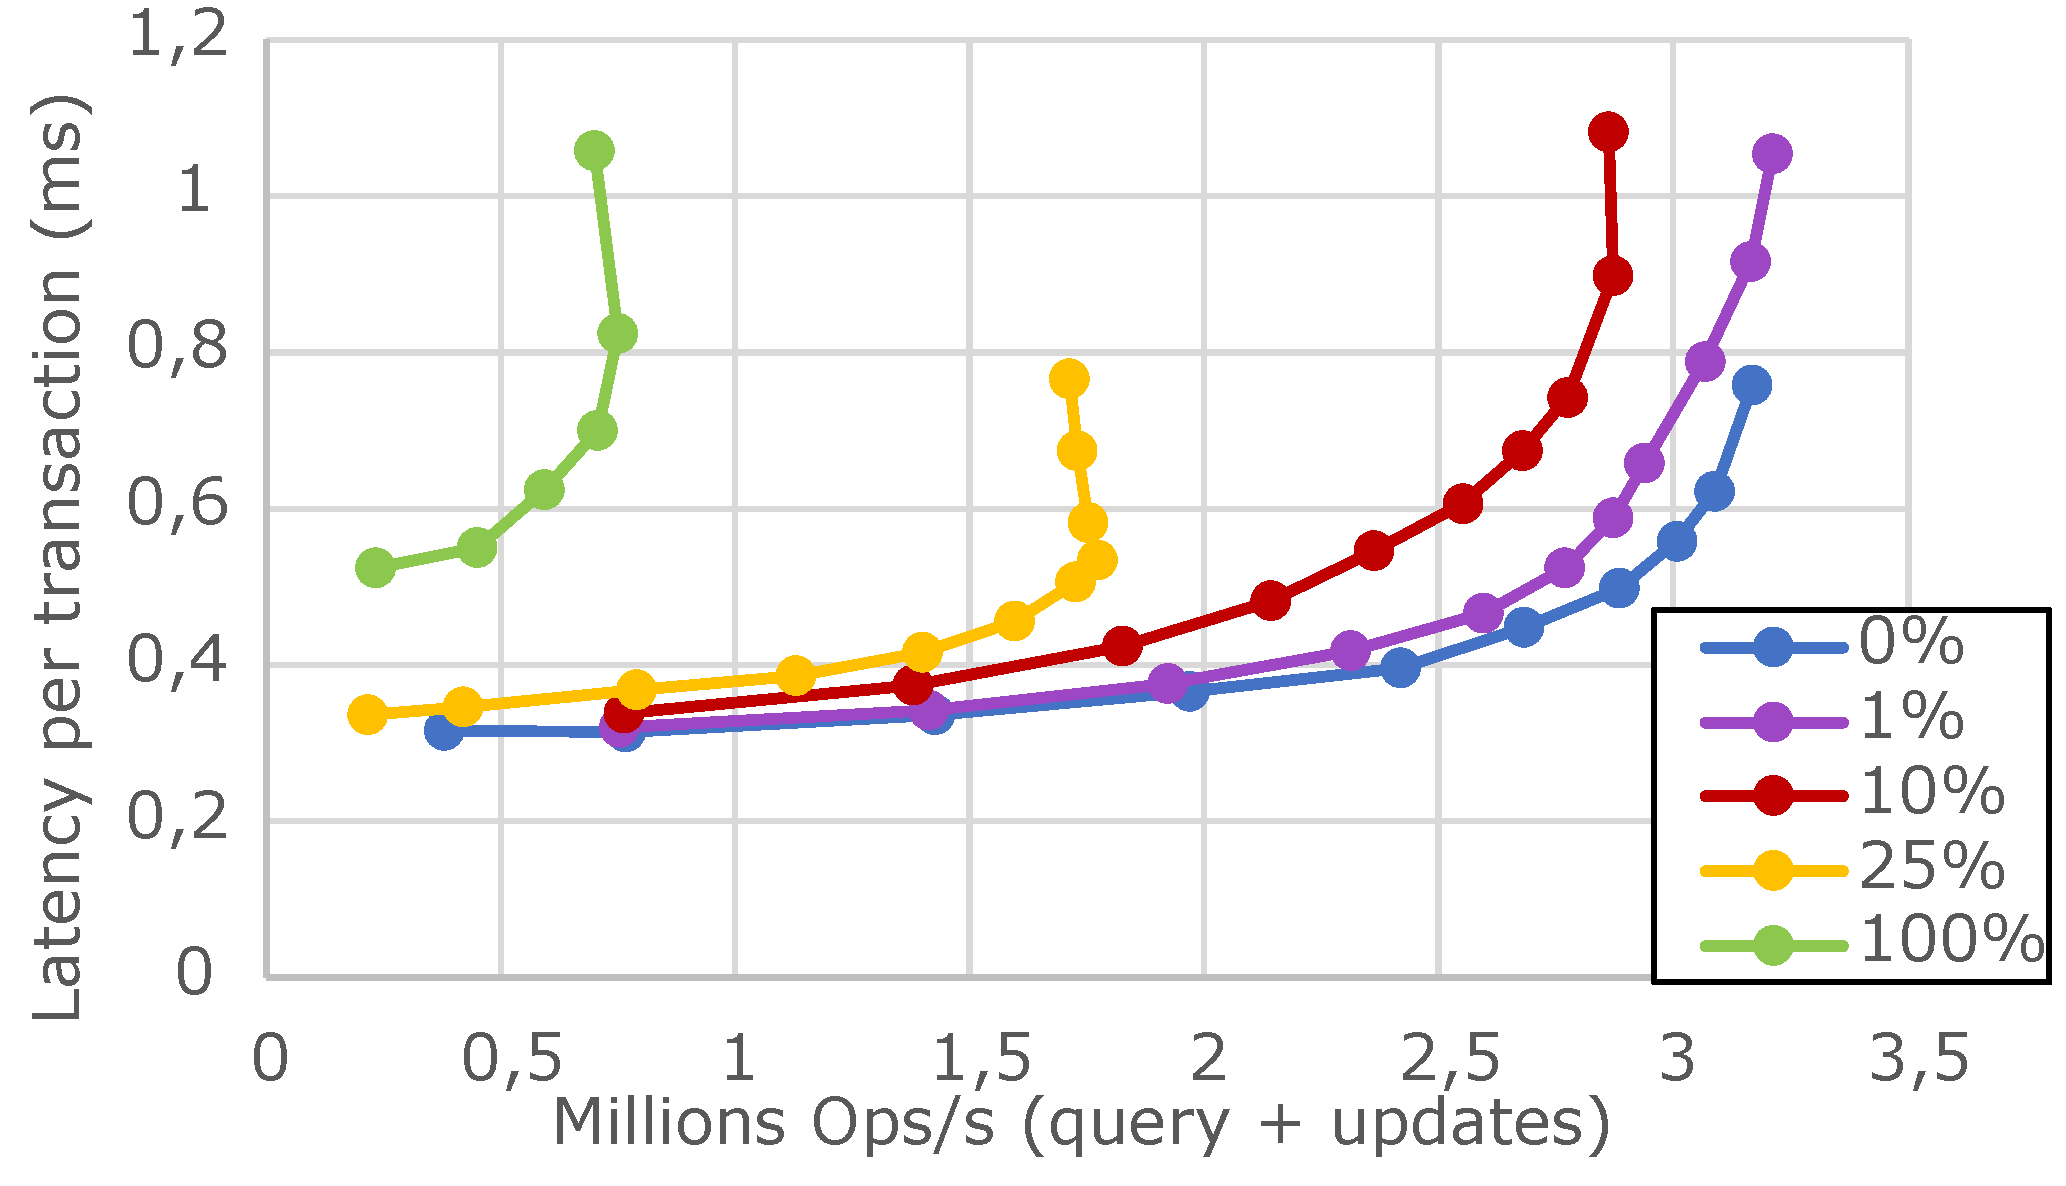
\includegraphics[width=.75\linewidth]{updRate_global_cut}
%	\caption{PotionDB's performance with varying update rate.}
%	\label{fig:(new_2)update_rates}
%\end{figure}
%\begin{figure}[h]
%	\centering
%	\begin{subfigure}{.5\linewidth}
%		\centering
%		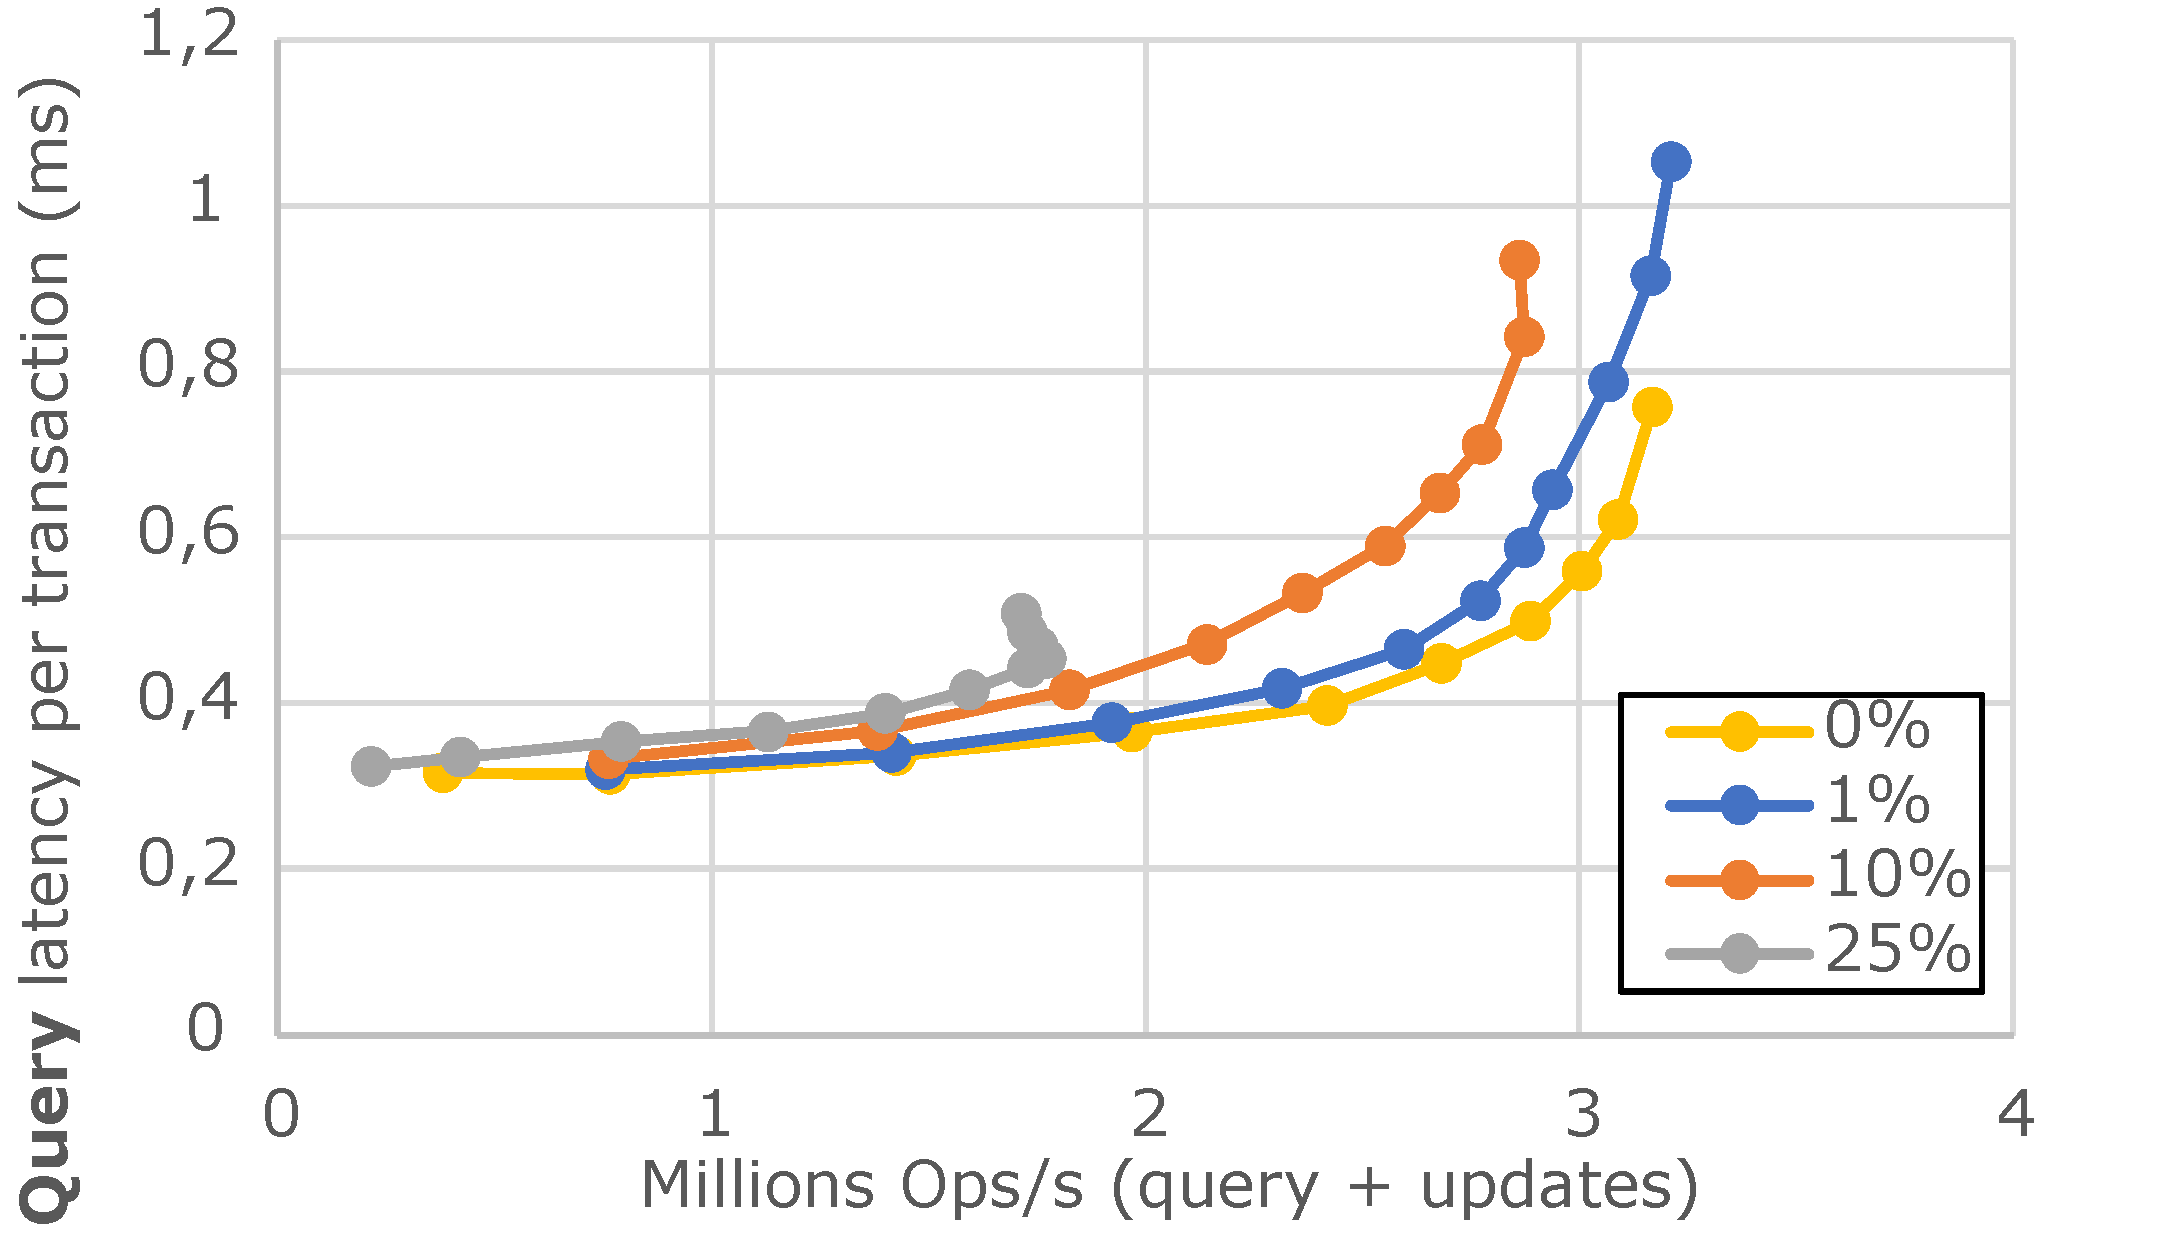
\includegraphics[width=.99\linewidth]{updRate_queryLatency_cut}
%		\caption{Query-latency}
%		\label{fig:(new)update_rates_query}
%	\end{subfigure}%
%	\begin{subfigure}{.5\linewidth}
%		\centering
%		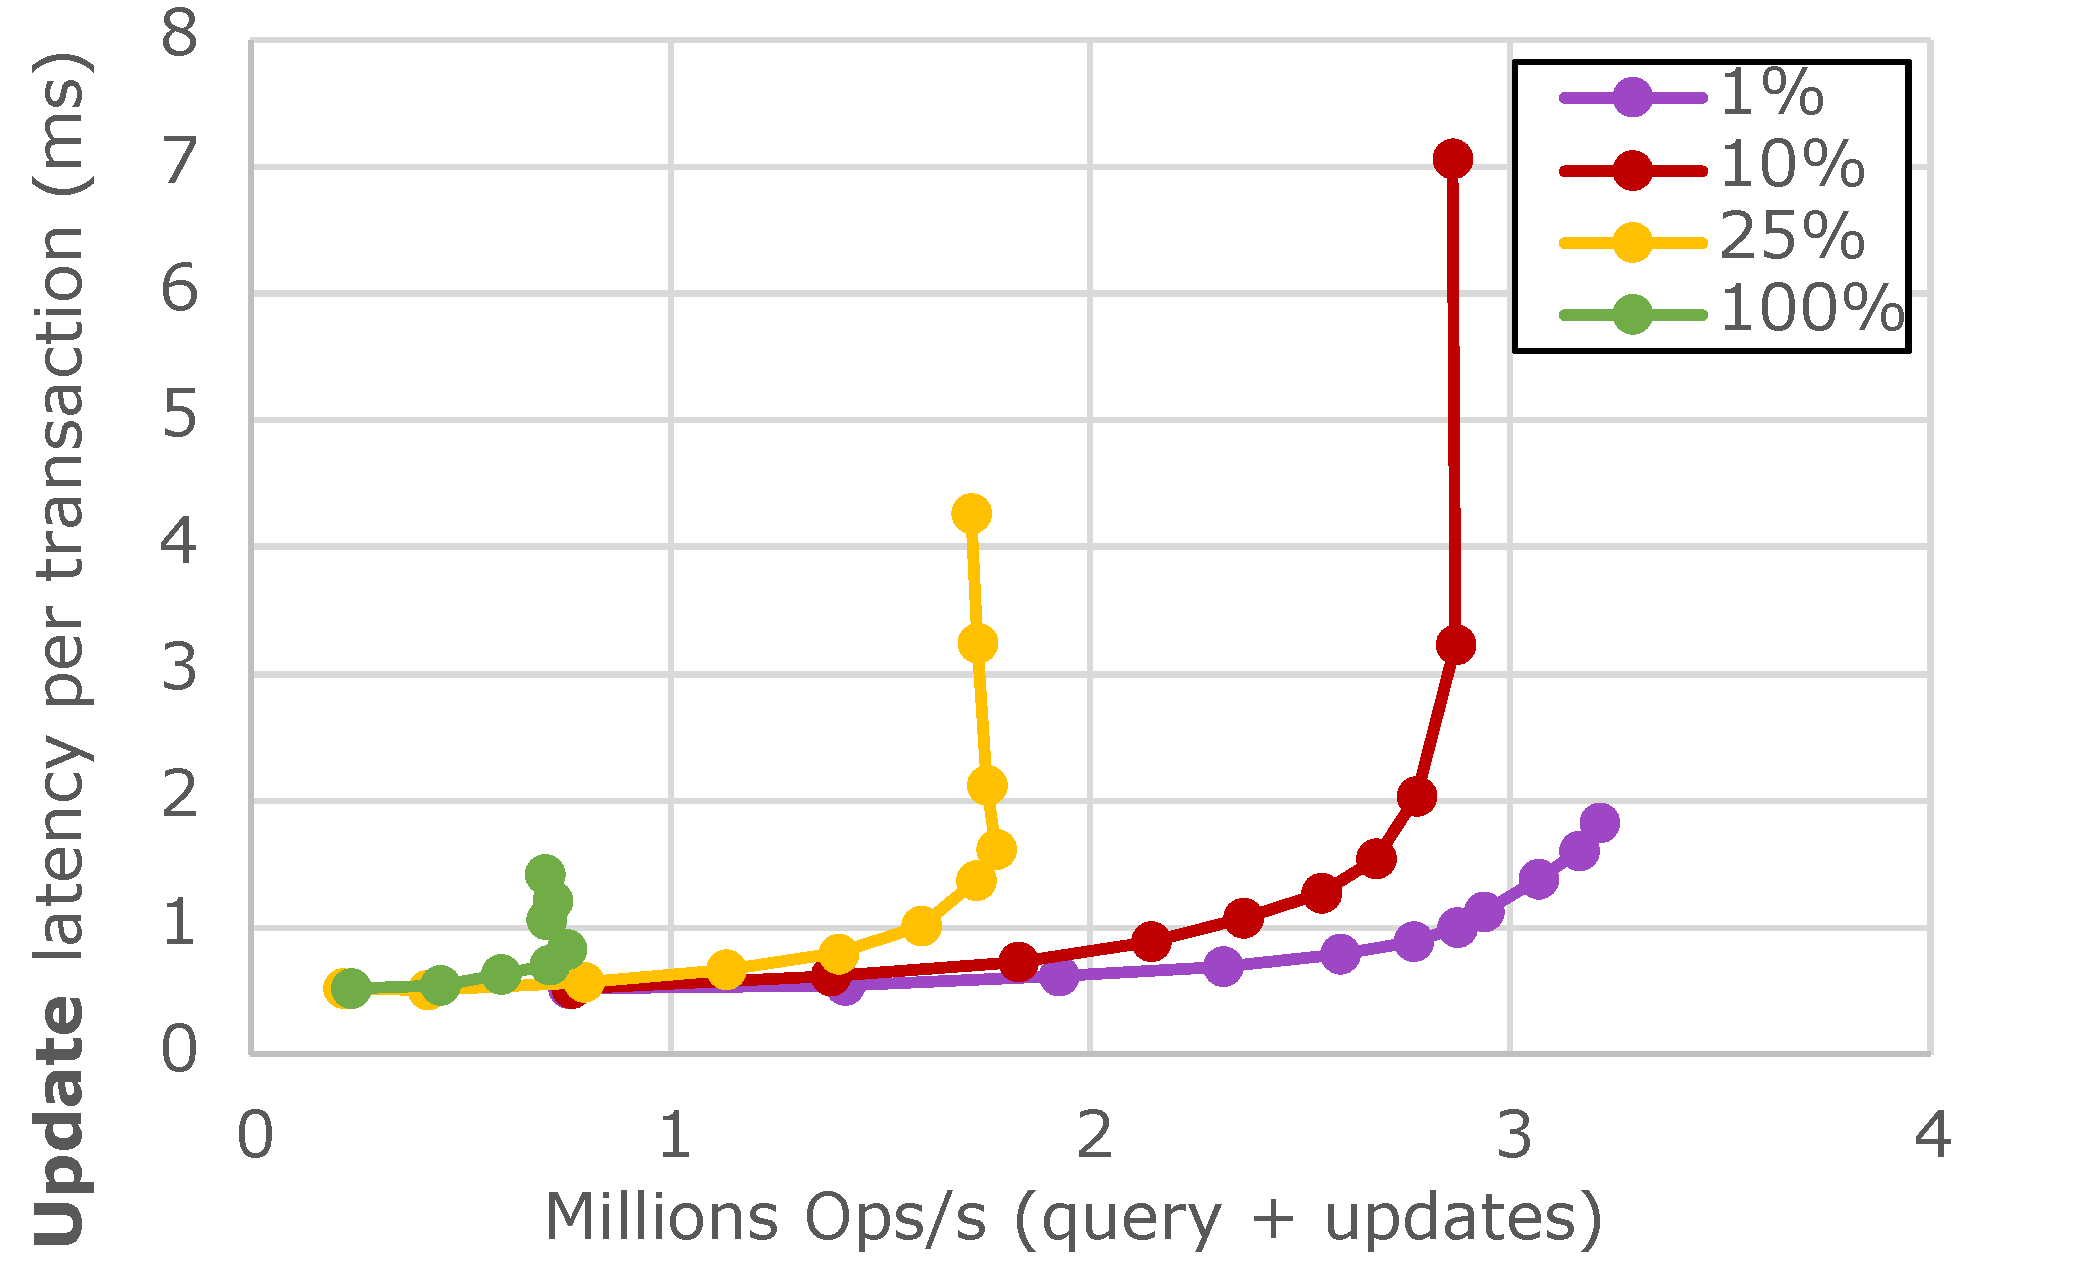
\includegraphics[width=.99\linewidth]{updRate_updateLatency_cut}
%		\caption{Update-latency}
%		\label{fig:(new)update_rates_update}
%	\end{subfigure}
%	\caption{PotionDB's performance with varying update rate, with query and update latencies split. Note that each update transaction adds and removes one order, as well as associated items and views, thus having more operations than one query-only transaction.}
%	\label{fig:(new)update_rates_split}
%\end{figure}
%
%\begin{figure}[h]
%	\centering
%	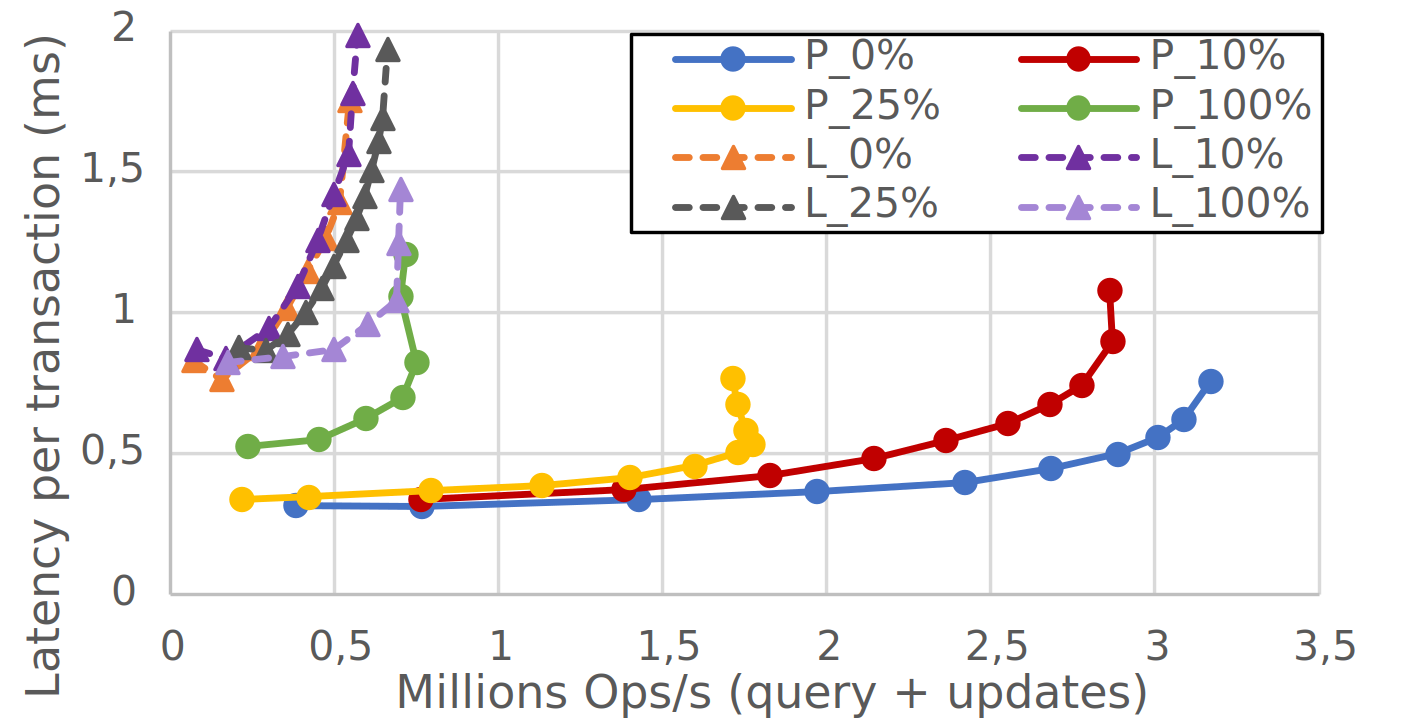
\includegraphics[width=.7\linewidth]{updRate_localvsglobal_cut}
%	\caption{Normal(P\_) and Local (L\_) PotionDB's performance with varying update rate.}
%	\label{fig:(new)update_rates_normal_vs_local}
%\end{figure}
%
%Note: Figure \ref{fig:(new_2)update_rates} is the same one as the one used in the latency section as... there is no visible difference.
%I could however re-run the experiments with latency to have maybe a very slightly difference. I suppose we won't repeat the graph.
%
%Note2: Are the graphs in Figure \ref{fig:(new)update_rates_split} still relevant? The idea is to differentiate how the latency of queries/updates scales. I believe it is.
%
%Note3: All the graphs still include in their throughput the view's updates. I will remove this later.
%
%\begin{itemize}
%	\item Mention how it can be observed that added latency has no effect on PotionDB's throughput with updates;
%	\item It is noticeable that updates have higher latency than queries even with few clients. This is mostly due to transactions with updates having more operations than query-only (due to needing to update order + its items + all views)
%	\item Latency on updates spikes more heavily at the end compared to queries. This is due to many concurrent transactions trying to commit, which makes each transaction having to wait for multiple others to finish before it is successfully committed. (I need suggestions to explain this one. Basically it's the problem of 2PC - too many transactions, they start conflicting and slow down the system. We don't use locks however.)
%	\item Not having latency added benefits local PotionDB. However, overall, its performance is still worse than PotionDB.
%	\item Local PotionDB's throughput increases slightly with the increase of the update ratio. This is because updates are not as hindered by views being split per region as queries. Half of our orders are local to a region, thus all updates of those half will be local-only. Even for orders that are not fully local, usually they only refer a subset of the other regions, thus only a few updates get redirected and to few servers. Furthermore, updates to the views do not need to be replicated and applied everywhere as all views are local.
%\end{itemize}
%
%IMPORTANT NOTE: After I remove the view's updates from the counting, it is possible that Local PotionDB no longer increases throughput with the \% of updates. However, it will still be worse than PotionDB for sure.

%\subsection{Types of views (or maybe, Views type benchmarking?}
\subsection{Scalability of different types of views}
\label{subsec:microbenchmarks}

We now try to assess how the CRDTs supporting different kinds of views scale.
We focus on what is most common in TPC-H: limits (TopK/TopSum) and aggregations, namely count and sum (Counter) and average (Average).
%We focus on the most common aggregations found on TPC-H: limits (TopK/TopSum), count and sum (Counter) and average (Average).

In this scenario we drop TPC-H's dataset and use instead micro-benchmarks.
For each test we prepare 20 CRDTs with random initial data.
TopKs and TopSums are initialized with 10k elements and never go beyond 10k.
We maintain the same number of servers (5) and replicate each CRDT in all servers.
Each client picks a CRDT randomly according to an uniform distribution and executes reads and possibly updates on it.
Unless stated otherwise, each client executes 5 operations per transaction, in order to avoid communication overheads of small messages dominating our experiments.


\begin{figure}
	\centering
	\begin{subfigure}{.481\linewidth}
		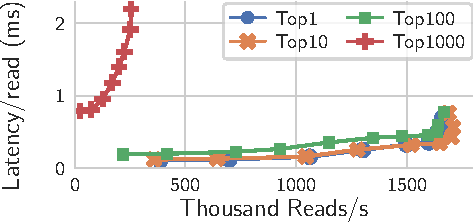
\includegraphics[width=1\linewidth]{singleQuery/bench_top_size_0_upd}
		\caption{1 read per txn.}
		\label{fig:topSize_single}
	\end{subfigure}%
	\hspace*{0.2em}
	\begin{subfigure}{.499\linewidth}
		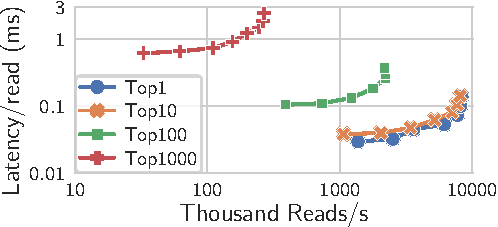
\includegraphics[width=1\linewidth]{singleQuery/bench_top_size_0_upd_5b}
		\caption{5 reads per txn (log scale).}
		\label{fig:topSize_batch}
	\end{subfigure}%
	%\vspace*{-0.65em}
	\caption{TopK query performance for multiple top sizes.}
	\label{fig:topSize}
	%\vspace*{-0.2em} %TODO: Increase this once we can pull higher the text
\end{figure}

%TODO: Need to replace the data for Top1 or Top10 in single read.
%For 5 batch: 8.339676e+06, 8.194999e+06, 2.211799e+06	, 2.676134e+05
%TODO: Maybe not focus so much on serialization/deserialization: it may not be easy to justify/not the real cause

\paragraph{TopK - K scalability and comparison with TopSum.} %\hspace{0em}

Figures \ref{fig:topSize_single} and \ref{fig:topSize_batch} showcase TopK's read performance for different values of K where clients execute, respectively, 1 and 5 reads per transaction.
Top1, Top10 and Top100 all perform similarly with 1 read per txn, as communication overhead for small messages (latency, metadata, serialization and deserialization of protobufs) and high number of clients dominate over costs of data transfer and query execution time.
%Top1, Top10 and Top100 all perform equally with 1 read per txn - this happens as the considerable communication overhead for such small requests and replies (latency, metadata transferred, serialization and deserialization of protobufs), together with the overhead of handling a high number of clients, dominates over the costs of data transfer and query execution time.
Grouping reads reduces the aforementioned overhead - with 5 reads per transaction, throughput from Top1 to Top10 drops very slightly ($\sim$2\%), with a much bigger drop for Top10 to Top100 ($\sim$73\%) and Top100 to Top1000 ($\sim$88\%).
In the latter two cases the amount of data transferred for the replies is the dominating factor, thus making better usage of the network's bandwidth.
We expect that after 1000, increasing K linearly will decrease throughput linearly as well.
%by the same factor.

%\begin{figure}
%	\centering
%	\begin{subfigure}{.49\linewidth}
%		\includegraphics[width=1\linewidth]{singleQuery/bench_top_size_0_1_5b}
%		\caption{10\% updates}
%		\label{fig:topSize_10_upd}
%	\end{subfigure}%
%	\hspace*{0.8em}
%	\begin{subfigure}{.49\linewidth}
%		\includegraphics[width=1\linewidth]{singleQuery/bench_top_size_0_25_5b}
%		\caption{25\% updates.}
%		\label{fig:topSize_25_upd}
%	\end{subfigure}
%	\caption{TopK performance for different top sizes and update rates.}
%	\label{fig:topSize_upd}
%\end{figure}

\begin{figure}
	\centering
	\includegraphics[width=0.76\linewidth]{singleQuery/topk_vs_topsum_5b}
	%\caption{TopK vs TopSum for multiple Top sizes and update ratios}
	\vspace*{-0.6em}
	\caption{TopK vs TopSum for various K and update ratios}
	\label{fig:topKVSTopSum}
	\vspace*{-0.75em}
\end{figure}

We now consider also the execution of updates for different values of K.
For updates, we use an add/remove ratio of 90\%/10\%, as it is unusual for tops/leaderboard-like objects to have frequent removes \cite{Cabrita17Nonuniform}.
Figure \ref{fig:topKVSTopSum} shows both TopK's and TopSum's max throughputs for multiple update/read ratios.
%Figure \ref{fig:topKVSTopSum} shows both TopK's and TopSum's max throughputs for update/read ratios of 0\%/100\%, 10\%/90\% and 25\%/90\%.
In all cases TopSum and TopK perform similarly.
%In all cases, despite TopSum's higher flexibility, its throughput is equivalent to TopK's.
%For now we focus only on TopK.
%Thus, we focus on TopK's scalability with updates.
Thus, we now focus on update scalability.
%The results with updates are somewhat different to query-only.
The size of an update is independent of the top's size - thus, as the amount of updates increase and reads decrease, throughput increases considerably for Top1000 and slightly for Top100.
%Although adding/removing elements gets more expensive as K increases (higher chance for the actual top to be modified), this is offset by the cost of transferring all K elements over the network as a read reply. 
%TODO: Would be nice to re-add the one above.
Conversely, Top1 and Top10's throughput decreases as the update ratio goes up, %as commits for updates lock shards, thus reducing read parallelism.
as commits for updates reduce read parallelism.

%We now consider also the execution of updates for different values of K.
%For updates, we use an add/remove ratio of 90\%/10\%, as it is unusual for Tops/leaderboard-like objects to have frequent removes \cite{Cabrita17Nonuniform}. %TODO: ACTUALLY USE THIS DATA AND REPLACE IT!
%Figure \ref{fig:topSize_upd} shows the results of executing 5 operations per transaction, with update/read ratios of 10\%/90\% and 25\%/75\%.
%The results here are somewhat different to a query-only scenario.
%Noteworthy, the amount of data transferred in an update is independent of the top size - thus, increasing the amount of updates (and thus decreasing the amount of queries) increases considerably the throughput of Top1000, while Top100 raises very slightly.
%Even though adding or removing an element gets more expensive the bigger K is (as it is more likely for an add or remove to change the top and thus for changes to need to be replicated), this is offset by the cost of transferring all the K elements over the network when answering queries. %Note: this isn't observable in the graphics because we do not have tests with 100% updates now.
%On the other hand, Top1 and Top10's throughput decreases as the update rate goes up, as transactions with updates must be committed (Section \ref{subsec:commit}) and thus reduces parallelism in query processing.

%TODO: I would love to leave this here but I feel like I should omit it. Or maybe make it even shorter
As a final note, without batching the throughput with updates keeps up better with the query-only scenario.
For instance, Top 10 with 0\% to 25\% updates goes from 8.19M to 2.23M (-72.8\%) and 1.7M to 1.12M (-34.1\%) ops/s for, respectively, 5 and 1 operations per transaction.
Multi-update transactions lock multiple shards instead of just one, so they reduce available parallelism more than single updates do.
%The higher drop is because multi-update transactions lock multiple shards instead of only one, thus reducing parallelism for commits and reads.
%As a final note, without batching of neither reads or updates the throughput with updates keeps up better with the query-only scenario.
%Namely, for Top10 with 0\%, 10\% and 25\% updates, with a single operation per transaction, Top10 achieves 1.7M, 1.27M (-25.3\%) and 1.12M (-34.1\%) ops/s, while with 5 operations per transaction it achieves 8.19M, 4M (-51.1\%) and 2.23M (-72.8\%) ops/s.
%This bigger difference is because update transactions with multiple updates can not commit as much in parallel as when only with a single update, as the former has to lock multiple shards instead of just one.

\paragraph{PotionDB scalability with number of replicas}

\begin{figure}
	\centering
	\begin{subfigure}{.325\linewidth}
		\includegraphics[width=1\linewidth]{singleQuery/n_servers_0_upd_5b}
		\caption{Query-only}
		\label{fig:crdts_0_upd}
	\end{subfigure}%
	\begin{subfigure}{.325\linewidth}
		\includegraphics[width=1\linewidth]{singleQuery/n_servers_0_1_upd_5b}
		\caption{10\% updates.}
		\label{fig:crdts_10_upd}
	\end{subfigure}%
	\begin{subfigure}{.34\linewidth}
	\includegraphics[width=1\linewidth]{singleQuery/n_servers_0_25_upd_5b}
	\caption{25\% updates.}
	\label{fig:crdts_25-upd}
	\end{subfigure}%
	\vspace*{-0.65em}
	\caption{Performance of Counter, Average and TopK}
	\label{fig:crdts}
	\vspace*{-0.8em}
\end{figure}

We now evaluate how TopK compares with Counter and Average, two CRDTs often used to implement aggregations and views.
%We now evaluate how TopK compares with other CRDTs often used to implement aggregations and views, namely Counter and Average. 
We also analyse how PotionDB scales with the number of replicas.
Figure \ref{fig:crdts} shows the throughput of said CRDTs under different numbers of replicas, with K = 10 for TopK.
All the analysed CRDTs have similar throughput as reads are quick to apply and produce small replies.
%All the analysed CRDTs have similar throughput, as reads are quick to apply, the amount of data transferred on Top10 is still small and updates for Top10 are cheap (aside from the commit cost common to all CRDTs).

%8.617347e+06
%6.920755e+06
%1.826504e+06
%2.572651e+06
%2.179531e+06
%665448.544308
%Since the three CRDTs behave similarly, we focus on Average to analyse scalability with number of replicas.
%For 0\% (resp. 25\%) updates, max throughputs go from 8.62M (resp. 2.57M) ops/s with 5 servers to 6.92M (resp. 2.17M) ops/s with 4 servers (-19.7\%, resp. -15.6\%) and to 1.83M (resp. 0.665M) ops/s with 1 server (-78.8\%, resp. -74.1\%).
%When executing only queries, throughput scalability is practically linear.
%However, with updates throughput scales less linearly, as updates have to be replicated and applied in every replicas.
%Despite the number of updates effectively applied in each server being more than 4 times higher with 5 replicas compared to 1 replica, the loss on scalability is modest.
%This is because PotionDB's replication mechanism groups updates from different transactions, allowing them to be applied more efficiently. %TODO: Maybe add reference to Replication section if I mention this there.

%PotionDB scales well both with and without updates.
With queries only, scalability is near linear on the number of replicas - e.g., Average with 1 server (1S) has 21.2\% of 5S' throughput of 8.62M ops/s.
With updates, max throughput is smaller and scalability is less linear - e.g., for 25\% updates, Average with 1S has 25.9\% of 5S' throughput of 2.57M ops/s.
PotionDB's scalability even with updates is solid given each replica applies around 4 times more updates with 5S than with 1S.
PotionDB's replication mechanism groups remote transactions together, allowing for efficient execution.
%When executing only queries, throughput scalability is close to linear as reads are locally served - e.g., Average goes from 8.62M ops/s with 5 servers (5S) to 6.92M ops/s with 4S (-19.7\%) and to 1.83M ops/s with 1S (-78.8\%).
%With updates, max throughput is lower and scales down less linearly, as updates must be propagated and executed in all replicas.
%E.g., Average with 25\% update rate goes from 2.57M ops/s with 5S to 2.17M ops/s with 4S (-15.6\%) and to 0.665M ops/s with 1S (-74.1\%).
%However, despite each replica applying around 4 times more updates with 5S than with 1S, the scalability loss is modest.
%%However, despite the number of updates effectively applied in each server being around 4 times higher with 5 replicas than with 1 replica, the loss on scalability is modest.
%This is because PotionDB's replication mechanism groups transactions together, allowing for efficient execution.
%This is because PotionDB's replication mechanism groups updates from different transactions, allowing them to be executed efficiently. %TODO: Maybe add reference to Replication section if I mention this there.
















%Maybe I really do not want to use batching for TopK size - as that favors our solution
%But then I have to test PotionDB with bigger top sizes, which is scary when considering updates.
%Note: Suggestions for the title above are welcome
%
%\begin{itemize}
%	\item We now evaluate the performance of CRDTs used to build the views of TPC-H: TopK, TopSum, Counter and Average.
%	\item Describe the new test scenario (as it is not TPC-H).
%\end{itemize}
%
%%TOPK test max throughputs: 11.3M, 10.3M, 3.1M, 0.37M
%\begin{figure}[h]
%	\centering
%	\includegraphics[width=.7\linewidth]{TopKTopSize0upd_cut}
%	\caption{TopK query performance with a varying top size.}
%	\label{fig:(new)TopkSize0upd}
%\end{figure}
%
%Describe differences in throughput, and justify. 1 -> 10: 10\% difference, as the amount of data transferred is small compared to communication overhead (latency + metadata transferred + cost of serialization/deserialization of protobufs), as well as the overhead of handling a high amount of clients. 10 -> 100, 10 -> 1000: 70\%, 88\%: the amount of data transferred is what weights the most. After 1000 we expect linear decrease of throughput.
%
%\begin{figure}[h]
%	\centering
%	\begin{subfigure}{.5\linewidth}
%		\centering
%		\includegraphics[width=.97\linewidth]{TopKTopSize25upd_cut}
%		\caption{TopK with 25\% updates}
%		\label{fig:(new)TopkSize25upd}
%	\end{subfigure}%
%	\begin{subfigure}{.5\linewidth}
%		\centering
%		\includegraphics[width=.97\linewidth]{TopKTopSize100upd_cut}
%		\caption{TopK with 100\% updates}
%		\label{fig:(new)TopkSize100upd}
%	\end{subfigure}
%	\caption{TopK operations (query + update) performance with varying top size.}
%	\label{fig:(new)TopkSize25_100upd}
%\end{figure}
%
%Note: Maybe the two graphs above (Figure \ref{fig:(new)TopkSize25_100upd}) is not needed? Maybe just Figure \ref{fig:(new)TopkVSTopsum} is enough.
%
%The differences between throughputs here is smaller compared to query-only scenarios.
%This is due to the amount of data transferred in updates being independent of the top's size.
%However, as expected, as the value of K increases, adding or removing elements to the top gets more expensive.
%(Possible justification: searching for the next element to put on the top after a remove is expensive, as the "not top" set of elements is unsorted. Higher Ks have this operation happen more often).
%
%\begin{figure}[h]
%	\centering
%	\includegraphics[width=.7\linewidth]{TopKVSTopSum_cut}
%	\caption{TopK and TopSum performances for different top sizes and update rates.}
%	\label{fig:(new)TopkVSTopsum}
%\end{figure}
%
%Performance is quite similar, except for high update rates, where TopSum performs considerably better.
%This is because TopSum does not have adds and removes but rather increments and decrements - when testing TopK with only adds and TopSum with only decrements, both CRDTs perform similarly.
%
%(Is the explanation above OK?)
%(Should the graph above include the latency? E.g. as a value on top of each bar.)
%
%\begin{figure}[h]
%	\centering
%	\begin{subfigure}{.33\linewidth}
%		\centering
%		\includegraphics[width=.97\linewidth]{CounterAvgTopK0upd_v2_cut}
%		\caption{0\% update rate}
%		\label{fig:(new)CounterAvgTopK0upd}
%	\end{subfigure}%
%	\begin{subfigure}{.33\linewidth}
%		\centering
%		\includegraphics[width=.97\linewidth]{CounterAvgTopK25upd_v2_cut}
%		\caption{25\% update rate}
%		\label{fig:(new)CounterAvgTopK25upd}
%	\end{subfigure}%
%	\begin{subfigure}{.33\linewidth}
%		\centering
%		\includegraphics[width=.97\linewidth]{CounterAvgTopK100upd_v2_cut}
%		\caption{100\% update rate}
%		\label{fig:(new)CounterAvgTopK100upd}
%	\end{subfigure}
%	\caption{Counter, Average and TopK CRDTs performance for different numbers of replicas and update rates.}
%	\label{fig:(new)CounterAvgTopK}
%\end{figure}
%
%\begin{itemize}
%	\item This test not only compares different types of views, it also shows a basic test of scalability of TPC-H with the number of replicas
%	\item The throughput on all three CRDTs is similar (when considering TopK as being Top1) - most of the cost is on communication, context switching (between clients) and 2PC (for updates). Updates for counters, averages and Tops of 1 are trivial.
%	\item For query-only, the performance scales near linearly with the number of servers for the three CRDTs. 5 to 1 server is a 78.8\% decrease.
%	\item With 100\% updates, the performance decreases less linearly: 5 to 4 servers is 17.1\% decrease, 5 to 1 is 67.9\%. This happens due to updates needing to be propagated and applied in every replica.
%	\item PotionDB's effective replication mechanism, namely the replication and appliance of groups of transactions at a time, allow replicated updates to be applied efficiently.
%\end{itemize}
%
%Notes: I do not have an explanation for TopK having slightly better performance than other CRDTs with 25\% updates.
%As for update-only having better throughput than updates+query, I can think of the following two possible reasons: a) updates make queries wait; b) update transactions reply quicker as a reply is sent as soon as a commit is confirmed, even if it is queued, unlike queries which have to wait for the result to be ready.

%\section{Evaluation}
%\label{sec:evaluation}
%
%In this section we conduct multiple experiments for evaluating PotionDB's performance.
%Namely, we try to assess the advantage of having, in each server, views that span data partitioned across multiple replicas.
%To this end we compare PotionDB with two other solutions.
%
%To showcase the difference between said solutions, consider a view $v$ concerning orders from all over the globe:
%
%\begin{compactitem}
%	\item \emph{PotionDB}: all servers replicate the view and $v$ is complete, i.e., considers all orders that are partitioned across servers;
%	\item \emph{Local view PotionDB}: each server contains views concerning only local data - e.g., on an european server, $v$ would only consider orders from european customers.
%	Thus, for queries concerning worldwide/multi-continent data, multiple servers have to be contacted to answer the query and extra processing logic to compute the result may be necessary;
%	\item \emph{Single view PotionDB}: only one server has all views, but the views are complete.
%	This can lead to great pressure in the server with views when updating base objects, as well as when querying views.
%	Moreover, faraway clients will experience high latency.
%\end{compactitem}
%
%%We compare PotionDB with a solution in which each server's view only reflects data replicated locally (local view PotionDB). In this solution, some queries may need to query multiple servers to aggregate all the necessary view data.
%%We also compare PotionDB with a solution in which one server hosts all the views, but those views are, similarly to PotionDB, of data partitioned across multiple replicas (single view PotionDB).
%%To exemplify the differences, consider a view concerning orders from all over the globe:
%%\begin{itemize}
%%	\item PotionDB: all servers replicate the view, and the view is complete, i.e., takes in consideration all orders, no matter where they are partitioned.
%%	\item Local view PotionDB: each server contains the view, but the view only concerns data replicated locally. E.g: an european server only replicates data or orders made in europe.
%%	In this example, if a query requires data from multiple continents, multiple servers have to be contacted to answer the query.
%%	\item Single view PotionDB: only one server contains the view, but the view is complete.
%%	This can lead to great pressure in the server with the view when updating objects related to the view and when querying views, as well as worse latency for faraway clients.	
%%\end{itemize}
%
%%In this section we conduct multiple experiments in order to evaluate PotionDB's performance.
%%Namely, we try to assess the advantage of all replicas having views spanning data partitioned across multiple replicas, instead of each replica having an incomplete view with only its local data (local PotionDB).
%%E.g., if we partition customer's data based on the continent of the customer's country, the local view of a server in Europe would only concern the data of european customers, while a global view would include customers from all over the globe.
%%We also compare PotionDB with a solution that has one server dedicated to host all views (single view PotionDB).
%
%\subsection{Settings}
%
%\subsubsection{Common settings}
%\label{subsubsec:commonSettings}
%
%In our tests a dataset based on TPC-H's dataset \cite{tpch} is used.
%Accurately, while we keep all the tables and use data generated by the dbgen tool \cite{tpch}, we focus only on a subset of the queries and, for each table, we only keep the columns necessary to answer such queries.
%The subset of queries used is described in Section \ref{subsec:implementedQueries}.
%
%
%In general, our test environment has the following configuration:
%%In general, our test environment is set up with the following configurations
%
%\begin{itemize}
%	\item Five PotionDB instances, each one executing in its own node. We also use another five nodes to execute the clients that will access PotionDB.
%	\item Each PotionDB instance replicates data concerning one continent.
%	Products, which are not location based, are replicated everywhere.
%	View replication works as previously described.
%%	\item The replication of views works as follows:
%%	\begin{enumerate*}[label=(\roman*)]
%%		\item PotionDB - all servers replicate all views, and the views contain data regarding all continents;
%%		\item Local view PotionDB - each server's views only concerns data regarding its own continent;
%%		\item Single view PotionDB - only one server replicates views, but said views contain data regarding all continents.
%%	\end{enumerate*}
%	\item All nodes contain 2x Intel Xeon Gold 6130 with 192 GB of RAM. All nodes are interconnected by a 10Gbps LAN.
%	\item Each client selects one server to execute queries upon and only contacts said server. For local view and single view PotionDBs, if a server cannot satisfy a query with its data, said server contacts other servers in order to reply to the query.
%	\item Clients communicate with a server using Google’s protobufs \cite{Protobufs} to serialize/deserialize data. PotionDB’s protobuf interface is an extension of AntidoteDB’s protobuf interface \cite{AntidoteDB}.
%	\item Unless otherwise specified, each request is a transaction which contains one instance of each query - this implies that, for local view PotionDB, transactions have more operations, as some queries need data from multiple regions.
%	\item In some scenarios, we impose latency between the servers, in order to simulate how PotionDB would perform when distributed across the globe.
%	We use as reference the latency between AWS instances, as measured in \cite{AWSLatency} \andre{(Add a date of access?)}.
%	The following regions were selected: EU (Paris), US (N.Virginia), Canada (Central), Asia Pacific (Tokyo), Middle East (Bahrain). The highest latency measured is between Canada and Middle East at 204ms as of the date of measure.
%	\andre{Note: a possible critic here is that we don't have one server per continent, which is the scenario we always describe in the paper.}
%	\andre{Second note: I rechecked the website - the latency between those two servers has improved a lot!!! Nowadays it is around 161ms. If I put a timeframe of 1 year it still shows 204ms, which suggests improvements in the connection. I probably need to reconsider the latencies?}
%\end{itemize}
%
%%Old settings for FCT's cluster
%%\begin{itemize}
%%	\item Five PotionDB instances, each one executing in its own node.
%%	Each node has a AMD EPYC 7281 CPU with 96GB of RAM, with PotionDB only being able to use 8 cores of the CPU (this helps ensure the bottleneck is not on the client side); \andre{Should I keep this?}
%%	\item Each PotionDB instance replicates the data of a continent, e.g., a server replicates all data concerning Europe while another keeps the data of Asia. Data that is not location based such as products is replicated in all servers, as are views.
%%	\item Servers are interconnected by a LAN with 10 Gbps speed;
%%	\item Clients execute on nodes with 2x Intel Xeon E5-2620 v2 CPU and 64GB of RAM, being on the same LAN as the servers but with a reduced network speed of 1Gbps;
%%	\item Each client selects one server to execute queries upon, only contacting other servers if all the data required to reply to a query isn't present in the selected server. \andre{Should I refer that, in practice, this only happens in the local views scenario?} By default, the queries executed are 3, 5, 11, 14, 15 and 18 of the TPC-H specification \cite{tpch};
%%	\item Unless otherwise specified, each request only executes one query or updates one sale (including all related views).
%%\end{itemize}
%
%All our experiments execute as follows.
%First, all servers are started, with each one estabilishing a connection with all others.
%Afterwards, the initial database state is loaded into the servers, taking into consideration data’s locality.
%%Afterwards, a special client is started to load the initial database state into the servers, taking into consideration the locality of the data.
%%Finally, after all data has been loaded into the servers, multiple clients are started to execute queries.
%%In some tests, a client responsible for updating the dataset (i.e., insert new elements and remove old ones) is also started along with the query clients.
%%We call this last client of update client.
%%In some other tests, all clients can do both queries and updates, with a varying percentage.
%Finally, after the loading phase ends, 
%%Finally, after all data has been loaded into the servers, 
%multiple clients are started to execute queries and/or updates, with the query/update rate depending on the test.
%
%In our experiments we use as metrics the amount of queries per second (query/s) achieved by all clients aggregated and the average latency of each transaction (including RTT).
%In tests with both updates and queries, we instead use operations per second (ops/s).
%To grasp how each test scales, we vary the number of clients.
%%To determine how much each test can scale, we vary the number of clients.
%As the number of clients increases, so does the latency of each transaction and, until the servers saturate, the throughput of the servers.
%
%\subsubsection{Scenarios}
%
%We make an extensive evaluation of PotionDB, conducting multiple experiments in order to evaluate how PotionDB scales in different scenarios. %When appropriate, we also execute the same experiments for local PotionDB and single view PotionDB.
%%With these experiments, we try to assess the following:
%With these experiments, we try to answer the following questions:
%
%%\begin{itemize}
%%	\item How does PotionDB compare with other solutions, namely the local and single versions of PotionDB? How does the data locality and size affect the performance?
%%	\item How much is PotionDB able to scale when executing queries only, or when trying to execute both queries and updates simultaneously?
%%	\item How does different read/write ratios affect PotionDB's performance?
%%	\item How well does each CRDT type scale in PotionDB, namelly when its size grows?
%%\end{itemize}
%\begin{enumerate}
%	\item \label{enum:question1} What is the practical benefict of having views of data replicated across different servers, compared to having only views of local data (local PotionDB) or a single view server (single PotionDB)?
%	\item \label{enum:question2}What is the effect on PotionDB's throughput of executing updates, namely as the write/read ratio increases?
%	%\item \label{enum:question3} \andre{Note: Before there used to be a section for how PotionDB scales by grouping operations. Now that doesn't seem to have much effect (about same throughput, but with less clients). But maybe this could help in the scenario with latency added. Should I still do this?}
%	\item\label{enum:question4}How does each kind of CRDT scale in PotionDB as we vary the number of clients, the number of replicas and other CRDT-specific settings (e.g., number of top elements in TopK CRDT)?
%	%\item\label{enum:question5}\andre{Any other question/evaluation?}
%\end{enumerate}
%
%\subsection{Results}
%
%\subsubsection{Locality of data}
%
%\andre{Is it worth to mention how much the number of clients vary by test?}
%
%To evaluate the benefits of having views replicated in every replica, we compare PotionDB with the local view and single view versions.
%Mainly, we try to assess how much each configuration scales in terms of throughput and latency, in order to grasp the benefict of having global views in every server.
%
%\begin{figure}
%	\centering
%	\begin{subfigure}{.5\linewidth}
%		\centering
%		\includegraphics[width=.9\linewidth]{clientScale_cut}
%		\caption{All queries}
%		\label{fig:global_local_single}
%	\end{subfigure}%
%	\begin{subfigure}{.5\linewidth}
%		\centering
%		\includegraphics[width=.9\linewidth]{Q3vsQ5_cut}
%		\caption{Single query type}
%		\label{fig:q3q5}
%	\end{subfigure}
%	\caption{Query-only performance of PotionDB and its local and single view versions. On the left all queries are executed, while on the right only Q3 or Q5 are.}
%	\label{fig:query_only}
%\end{figure}
%
%Figure \ref{fig:query_only} shows the results of experiments for the three versions of PotionDB, in terms of query/s versus latency.
%Figure \ref{fig:global_local_single} includes all queries in the execution, while \ref{fig:q3q5} only includes a single type of query at a time.
%
%When factoring in all queries (Figure \ref{fig:global_local_single}), as expected both local and single view PotionDB perform worse than (normal) PotionDB.
%The single version's max throughput is about 1/5th of PotionDB's.
%This occours due to queries being entirely served by views, which are all in a single server - thus, in a query-only scenario, one server gets all the load, instead of it being distributed across 5 servers.
%The local version has about 1/6th of PotionDB's performance, as 2/3rd of the queries require data from all regions, which implies that in local mode such queries need to consult the views in every server.
%The redirection of requests (see Section \ref{subsec:operationsNonLocal}) required to consult the views of others servers implies an extra round-trip for most queries. It also implies waiting for all servers to reply in order to complete a transaction, further reducing thoughput and increasing latency.
%
%In Figure \ref{fig:q3q5} the focus is on two particular queries. Query 3 (Q3) requires data from all over the globe, while Query 5 (Q5) can be answered with data from a single region.
%Thus, Q5 fits well both normal and local versions of PotionDB.
%In fact, Q5's performance in local and normal modes is very similar - both reach a max throughput of around 4 million queries/s.
%This occours as clients query data concerning the region of the server they are connected to, thus there is no need to contact other servers even in the local version.
%As for the single version, Q5's performance is about 1/5th of the other two.
%On the other hand, Q3 is a perfect example of how data locality affects performance.
%This query requires data from all servers, thus in the local version every server needs to be contacted. The extra pressure on the servers (as all servers are required to answer all queries), as well as the extra round-trip, alongside bigger transfers of data, lead to a decreased performance of about 1/13th compared to PotionDB.
%The single version has, as expected, about 1/5th of PotionDB's performance.
%
%\begin{figure}
%	\centering
%	\includegraphics[width=.75\linewidth]{clientScale_tc_cut}
%	\caption{PotionDB's performance executing all queries with added latency. Both axes have a log(10) scale.}
%	\label{fig:global_local_single_tc}
%\end{figure}
%
%In the previous tests the latency of the clients to all servers is very low, as all servers and clients are connected in a LAN.
%Figure \ref{fig:global_local_single_tc} shows the result of adding latency between servers (clients still retain low latency to represent being close to their server of choice).
%Normal PotionDB is "unnafected" in terms of throughput and client's latency as clients only contact their nearby server - since no latency is added between client-server, no effect is noticeable.
%In a scenario with updates however, an effect would be noticeable "under the hood" - replication would take longer to happen due to the imposed latency, thus a given client would take longer to be able to see the effects of updates executed on servers other than the one said client is connected to.
%This would not affect query throughput, instead only the freshness of data.
%For single PotionDB, a higher latency is noticeable compared to Figure \ref{fig:global_local_single}.
%This happens as most clients will have high latency (i.e., the ones not connected to the server with the views) and do few operations, while the remaining ones will be operating directly on the view server.
%The ones operating directly will be responsible for the majority of the load in the server with views - hence why the average client's latency increased midly.
%As such, as long as more clients are used compared to Figure \ref{fig:global_local_single}, a similar max throughput is still achieved.
%Finally, it is on local PotionDB where the effects of latency are most noticeable - here, for 2/3rd of the queries, all servers will be contacted. Since all transactions consist in one of each type of query, this implies all transactions will take, at least, as long as a RTT between the two most faraway servers - hence the observed latency of about 210ms.
%Compared to Figure \ref{fig:global_local_single}, the max throughput is much lower. This is due to the much higher amount of clients needed to sature the servers: aproximately 3000 clients instead of 160.
%The much higher amount of connections to each server, as well as the much more frequent "swap" of the processor cores between each client justify this lower throughput.
%
%\subsubsection{PotionDB scaling - queries VS updates}
%
%We now evaluate the impact on PotionDB's throughput of executing updates alongside queries, with multiple read/write ratios (\ref{enum:question2}).
%In this scenario, when a client wants to execute an operation, it picks at random whenever a query or an update is executed.
%
%In TPC-H an update is defined as the replacement of an old order with a new one.
%As such, our granularity of update is the addition and removal of an order, with the associated items and necessary views' updates.
%Finally, it is worth noting that even though some updates will execute in multiple replicas (e.g.: view updates), we only count one execution in our graphs.
%%It is worth noting that an update affects both base data and all associated views.
%%Also note that while view updates are executed in every replica, we only count them once (i.e., if one update is executed 5 times, it still only counts as 1 operation).
%
%\begin{figure}
%	\centering
%	\includegraphics[width=.75\linewidth]{updRate_global_cut}
%	\caption{PotionDB's performance with varying update rate.}
%	\label{fig:update_rates}
%\end{figure}
%\begin{figure}
%	\centering
%	\begin{subfigure}{.5\linewidth}
%		\centering
%		\includegraphics[width=.99\linewidth]{updRate_queryLatency_cut}
%		\caption{Query-latency}
%		\label{fig:update_rates_query}
%	\end{subfigure}%
%	\begin{subfigure}{.5\linewidth}
%		\centering
%		\includegraphics[width=.99\linewidth]{updRate_updateLatency_cut}
%		\caption{Update-latency}
%		\label{fig:update_rates_update}
%	\end{subfigure}
%	\caption{PotionDB's performance with varying update rate, with query and update latencies split. Note that each update transaction adds and removes one order, as well as associated items and views, thus having more operations than one query-only transaction.}
%	\label{fig:update_rates_split}
%\end{figure}
%
%Figure \ref{fig:update_rates} shows the results of executing updates alongside queries, with varying odds of choosing an update.
%For low update rates (1\% and 10\%), the decrease in performance can be considered reasonable: aproximately 4\% and 16\%.
%For higher rates, two observations can be made:
%\begin{enumerate*}[label=(\roman*)]
%	\item the servers saturate earlier, in some cases even decreasing throughput as the number of clients rises;
%	\item the max throughput is lower.
%\end{enumerate*}
%
%The referred observations can be explained by considering the following. 
%With PotionDB's sharding (Section \ref{subsec:sharding}), queries on objects of different shards can be executed concurrently, thus query-only scenarios scale easily. 
%However, transactions with updates must lock the partitions they are involved and do our commit protocol in order to ensure the states evolve sequentially in a replica even when concurrent transactions are issued.
%As such, if the update rate is high, clients executing queries or updates may often have to wait for a transaction with updates to finish executing before executing their own operations.
%
%Figure \ref{fig:update_rates_split} shows the same experiment as Figure \ref{fig:update_rates}, but showcases the latencies of queries and updates splitted, instead of together.
%It is noticeable that updates, even with few clients, have higher latency than queries - this is mostly due to update transactions having more operations than queries.
%The abrupt spike observed at the end in the update latency graph happens as many clients are doing updates and, thus, many commits with locks are issued, which have to wait for each other to finish.
%
%\begin{figure}
%	\centering
%	\includegraphics[width=.7\linewidth]{updRate_localvsglobal_cut}
%	\caption{Normal(P\_) and Local (L\_) PotionDB's performance with varying update rate.}
%	\label{fig:update_rates_normal_vs_local}
%\end{figure}
%
%\andre{Note: I'm not sure on the explanation below. Basically, in local mode, more update ops are done per transaction, thus actually less orders are updated in the same period of time. However, since views are local, there's less replication work. Not much redirection is done as 50\% of the orders are fully local, and most others have few regions.}
%
%Figure \ref{fig:update_rates_normal_vs_local} showcases the performance of both PotionDB and local PotionDB with varying update rates.
%As expected, local PotionDB performs worse than PotionDB.
%However, as the percentage of updates increases in local PotionDB, so does the throughput.
%This happens as updates are not as hindered by views being split per region as queries.
%Aproximately half of the orders are local to a region \footnote{This does not occour on the original TPC-H dataset, whose items of orders are totally random. We did this modification to add locality to orders. This helps local PotionDB more than PotionDB.} while most others refer few regions, thus not many view updates need to be redirected to other servers.
%Besides, since each view only contains local data, updates to a view do not need to be replicated to every other server, reducing the load on the servers due to replication.
%These factors added up allow local PotionDB to have higher performance when updates are added and end up with a similar throughput to PotionDB when only updates are executed.
%
%\andre{Maybe a graph of local VS normal PotionDB with updates of all views and only queries of Q5? That query has high performance in both modes - may be interesting to see how it scales with updates (I wonder if local PotionDB has higher throughput than normal in that scenario?)}
%
%We now consider a scenario with latency added between servers, as described in Section \ref{subsubsec:commonSettings}.
%Recall that on normal PotionDB, as previously discussed, throughput isn't affected as clients only interact with the server they are close to, even when doing updates.
%They would, however, take longer to see the effects of updates done on views that were executed in other servers, due to the added latency on replication.
%
%\begin{figure}
%	\centering
%	\includegraphics[width=.7\linewidth]{updRate_tc_cut}
%	\caption{Local PotionDB's performance with varying update rate, with latency added.}
%	\label{fig:update_rates_tc}
%\end{figure}
%
%Thus, we focus on local PotionDB, which is shown on Figure \ref{fig:update_rates_tc}.
%We can easily observe that as the percentage of updates rise, the maximum throughput also rises quickly.
%At a first glance this may seem confusing, however the following justifies this behavior:
%\begin{compactitem}
%	\item Updates have lower latency than queries, as each update transaction only needs to contact a subset of servers, unlike query transactions which need to contact all. Thus, they can often avoid the connection with highest latency.
%	\item Updates have more operations per transaction than queries, which means more operations done per round trip.
%\end{compactitem}
%
%\andre{Should I mention that a lot less clients are needed to sature the server, the higher the update rate is? (mainly on scenarios without latency)}
%\andre{Probably some concluding note that reffers that for PotionDB's intented usages it is likely that updates are much less frequent than queries, or maybe even that updates could maybe be delayed?}
%
%\subsubsection{CRDT Benchmarks}
%
%%\andre{Note: On the graphs here I forgot to put "Latency per transaction (ms)" instead of just "Latency (ms)"... will fix that when we do a final version of those graphs}
%
%We now focus on evaluating the performance of the CRDTs used to build the views of TPC-H.
%Namely, we test TopK, TopSum, Counter and Average CRDTs.
%\andre{TODO: Maybe I should test embedded maps too? Since they are used to ``hold'' multiple CRDTs in Q5, acting as a group by.}
%
%In this scenario, we drop the TPC-H dataset.
%Instead, for each test we prepare 20 CRDTs with random initial data (the same amount of CRDTs used for Q15’s views, discussed in Section \ref{subsec:implementedQueries}).
%%Instead, we prepare each CRDT with some random initial data.
%%In each test, 20 CRDTs are created/manipulated by the clients (the same number of CRDTs that are used to build the views for Query 15, discussed in Section \ref{subsec:implementedQueries}).
%Each client picks a CRDT randomly following an uniform distribution and uses said CRDT to do query and/or update operations. 
%%Then, each client does query and/or update operations on one of the CRDTs.
%The number of operations per transaction is the same as in the TPC-H scenario. \andre{(Do I need to define this in the TPC-H scenario?)}
%%The distribution of CRDTs is the type "shared"
%
%
%%TOPK test max throughputs: 11.3M, 10.3M, 3.1M, 0.37M
%\begin{figure}
%	\centering
%	\includegraphics[width=.7\linewidth]{TopKTopSize0upd_cut}
%	\caption{TopK query performance with a varying top size.}
%	\label{fig:TopkSize0upd}
%\end{figure}
%
%Figure \ref{fig:TopkSize0upd} contains the results of executing TopK queries with different values for K.
%The throughput difference between Top-1 and Top-10 is small (10\%). This happens as the amount of data transfered is small compared to the communication overhead (latency + metadata transfered, alongside the cost of serializing/parsing the protobufs for request and reply), as well as the overhead of handling a high amount of clients.
%As the size of the TopK increases, the query performance drops as the amount of data transfered starts to become more relevant.
%From Top-10 to Top-100 and Top-100 to Top-1000 the throughput decreases by, respectively, 70\% and 88\%.
%We expect that after 1000, increasing linearly the number of elements on top will decrease the throughput by the same factor.
%%\andre{Should I mention throughput numbers? The max of each is 11.3M, 10.3M, 3.1M, 0.37M ops/s.}
%%\andre{Is it relevant to mention the number of entries in the TopK? (10000, same as in Q15) If so, how/where do I mention that?}
%
%\begin{figure}
%	\centering
%	\begin{subfigure}{.5\linewidth}
%		\centering
%		\includegraphics[width=.97\linewidth]{TopKTopSize25upd_cut}
%		\caption{TopK with 25\% updates}
%		\label{fig:TopkSize25upd}
%	\end{subfigure}%
%	\begin{subfigure}{.5\linewidth}
%		\centering
%		\includegraphics[width=.97\linewidth]{TopKTopSize100upd_cut}
%		\caption{TopK with 100\% updates}
%		\label{fig:TopkSize100upd}
%	\end{subfigure}
%	\caption{TopK operations (query + update) performance with varying top size.}
%	\label{fig:TopkSize25_100upd}
%\end{figure}
%
%
%Figure \ref{fig:TopkSize25_100upd} contains the same test as before but with, respectively, 25\% and 100\% updates.
%The differences in performance here are different compared to query-only's scenario.
%This happens as on updates, the amount of data transfered is similar for all scenarios. 
%However, as expected, as the value of K increases, adding or removing elements to the top gets more expensive.
%\andre{Not sure if/how I explain this. I believe the reason why it becomes more expensive is because of when the TopK needs to search for the ``new minimum'' of the top - since the elements ``not in top'' are stored as a set, sometimes that entire set needs to be searched upon to find a new minimum.}
%
%%\andre{Note: Interestingly, the TopSum graphs for 100\% updates are quite different from TopK. TopSum scores 5M ops/s on all top sizes for 100\% updates (to be precise: 5.4M, 5.4M, 5.3M, 5.1M Top1, Top10, Top100, Top1000); while TopK scores below 2M ops/s for Top1000. I haven't searched yet why it is like that.}
%
%\begin{figure}
%	\centering
%	\includegraphics[width=.7\linewidth]{TopKVSTopSum_cut}
%	\caption{TopK and TopSum performances for different top sizes and update rates.}
%	\label{fig:TopkVSTopsum}
%\end{figure}
%
%Figure \ref{fig:TopkVSTopsum} shows how the TopSum compares to the TopK CRDT in similar scenarios.
%When only executing queries, the performance is very similar. 
%However for high update rates, TopSum handles updates better than TopK.
%This is because TopSum does not have adds and removes but rather increments and decrements - when testing TopK with only adds and TopSum with only increments, both CRDTs perform similarly.
%%When we test TopK with only adds and TopSum with only increments, both CRDTs have very approximate throughputs (4.8M and 5M ops/s with 100% update rate for, respectively, TopK and TopSum).
%%I am not sure what causes the high overhead when removals are considered in TopK that doesn't affect decrements in TopSum. There's some ideas below
%%1- TopSum doesn't have removes but rather incs/subs, so less elements being removed/created from each set (but still, some should when moved between top and not-top) ; 2 - topK has tombstones, topSum does not (but should be okay as it is only 1 timestamp per element) ; 3 - TopSum uses pointers to structures for the elements while TopK uses structures ; 4 - some other reason? Like different behaviour? I don't know. Maybe I need to test with a Map or Set CRDT. But even so it is odd...}
%
%\begin{figure}
%	\centering
%	\begin{subfigure}{.33\linewidth}
%		\centering
%		\includegraphics[width=.97\linewidth]{CounterAvgTopK0upd_v2_cut}
%		\caption{0\% update rate}
%		\label{fig:CounterAvgTopK0upd}
%	\end{subfigure}%
%	\begin{subfigure}{.33\linewidth}
%		\centering
%		\includegraphics[width=.97\linewidth]{CounterAvgTopK25upd_v2_cut}
%		\caption{25\% update rate}
%		\label{fig:CounterAvgTopK25upd}
%	\end{subfigure}%
%	\begin{subfigure}{.33\linewidth}
%		\centering
%		\includegraphics[width=.97\linewidth]{CounterAvgTopK100upd_v2_cut}
%		\caption{100\% update rate}
%		\label{fig:CounterAvgTopK100upd}
%	\end{subfigure}
%	\caption{Counter, Average and TopK CRDTs performance for different numbers of replicas and update rates.}
%	\label{fig:CounterAvgTopK}
%\end{figure}
%
%Figure \ref{fig:CounterAvgTopK} shows the max throughput of Counter, Average, and TopK (top of one) CRDTs.
%In these tests we try to assess how the performance of CRDTs scales with the number of replicas.
%When executing queries-only, the performance scales aproximately linearly with the number of servers for the three CRDTs, with all three CRDTs having similar throughput.
%For instance, Average CRDT goes from 11.1M ops/s with 5 servers to 2.35M ops/s with 1 server (78.8\% decrease).
%This happens as any server can be queried without needing to synchronize with other servers.
%With updates, the max throughput is lower and it scales down less linearly.
%For example, Average CRDT with 25\% update rate goes from 3.46M ops/s with 5 servers to 2.87M ops/s with 4 servers (17.1\% decrease) and to 1.11M ops/s with 1 server (67.9\% decrease from 5 servers).
%A similar percentage drop is observed with 100\% updates.
%This happens as updates have to be propagated and executed in every other replica.
%However, PotionDB's replication mechanism groups updates from different transactions, allowing them to be executed more efficiently.
%\andre{No idea why topK has a bit more performance with 25\% updates. I'm not sure why update-only has better throughput than query+update, but I can think of two possible reasons: a) updates make queries wait; b) updates reply quicker as a reply is sent as soon as the partitions confirm they will commit (and not after the commit is executed), unlike queries which must wait for the result to be ready.}
